% ******************************* PhD Thesis Template **************************
% Please have a look at the README.md file for info on how to use the template

\documentclass[a4paper,12pt,times,numbered,print,index,custommargin]{PhDThesisPSnPDF}

% ******************************************************************************
% ******************************* Class Options ********************************
% *********************** See README for more details **************************
% ******************************************************************************

% `a4paper'(The University of Cambridge PhD thesis guidelines recommends a page
% size a4 - default option) or `a5paper': A5 Paper size is also allowed as per
% the Cambridge University Engineering Deparment guidelines for PhD thesis
%
% `11pt' or `12pt'(default): Font Size 10pt is NOT recommended by the University
% guidelines
%
% `oneside' or `twoside'(default): Printing double side (twoside) or single
% side.
%
% `print': Use `print' for print version with appropriate margins and page
% layout. Leaving the options field blank will activate Online version.
%
% `index': For index at the end of the thesis
%
% `draftclassic': For draft mode without loading any images (same as draft in book)
%
% `draft': Special draft mode with line numbers, images, and water mark with
% timestamp and custom text. Position of the text can also be modified.
%
% `abstract': To generate only the title page and abstract page with
% dissertation title and name, to submit to the Student Registry
%
% `chapter`: This option enables only the specified chapter and it's references
%  Useful for review and corrections.
%
% ************************* Custom Page Margins ********************************
%
% `custommargin`: Use `custommargin' in options to activate custom page margins,
% which can be defined in the preamble.tex. Custom margin will override
% print/online margin setup.
%
% *********************** Choosing the Fonts in Class Options ******************
%
% `times' : Times font with math support. (The Cambridge University guidelines
% recommend using times)
%
% `fourier': Utopia Font with Fourier Math font (Font has to be installed)
%            It's a free font.
%
% `customfont': Use `customfont' option in the document class and load the
% package in the preamble.tex
%
% default or leave empty: `Latin Modern' font will be loaded.
%
% ********************** Choosing the Bibliography style ***********************
%
% `authoryear': For author-year citation eg., Krishna (2013)
%
% `numbered': (Default Option) For numbered and sorted citation e.g., [1,5,2]
%
% `custombib': Define your own bibliography style in the `preamble.tex' file.
%              `\RequirePackage[square, sort, numbers, authoryear]{natbib}'.
%              This can be also used to load biblatex instead of natbib
%              (See Preamble)
%
% **************************** Choosing the Page Style *************************
%
% `default (leave empty)': For Page Numbers in Header (Left Even, Right Odd) and
% Chapter Name in Header (Right Even) and Section Name (Left Odd). Blank Footer.
%
% `PageStyleI': Chapter Name next & Page Number on Even Side (Left Even).
% Section Name & Page Number in Header on Odd Side (Right Odd). Footer is empty.
%
% `PageStyleII': Chapter Name on Even Side (Left Even) in Header. Section Number
% and Section Name in Header on Odd Side (Right Odd). Page numbering in footer

% Uncomment to change page style
%\pagestyle{PageStyleII}

% ********************************** Preamble **********************************
% Preamble: Contains packages and user-defined commands and settings
% ******************************************************************************
% ****************************** Custom Margin *********************************

% Add `custommargin' in the document class options to use this section
% Set {innerside margin / outerside margin / topmargin / bottom margin}  and
% other page dimensions
\ifsetCustomMargin
	\RequirePackage[left=30mm,right=20mm,top=20mm,bottom=20mm]{geometry}
	\setFancyHdr % To apply fancy header after geometry package is loaded
\fi

% Add spaces between paragraphs
%\setlength{\parskip}{0.5em}
% Ragged bottom avoids extra whitespaces between paragraphs
\raggedbottom
% To remove the excess top spacing for enumeration, list and description
%\usepackage{enumitem}
%\setlist[enumerate,itemize,description]{topsep=0em}

% *****************************************************************************
% ******************* Fonts (like different typewriter fonts etc.)*************

% Add `customfont' in the document class option to use this section

\ifsetCustomFont
  % Set your custom font here and use `customfont' in options. Leave empty to
  % load computer modern font (default LaTeX font).
  %\RequirePackage{helvet}

  % For use with XeLaTeX
  %  \setmainfont[
  %    Path              = ./libertine/opentype/,
  %    Extension         = .otf,
  %    UprightFont = LinLibertine_R,
  %    BoldFont = LinLibertine_RZ, % Linux Libertine O Regular Semibold
  %    ItalicFont = LinLibertine_RI,
  %    BoldItalicFont = LinLibertine_RZI, % Linux Libertine O Regular Semibold Italic
  %  ]
  %  {libertine}
  %  % load font from system font
  %  \newfontfamily\libertinesystemfont{Linux Libertine O}
\fi

% *****************************************************************************
% **************************** Custom Packages ********************************

% ************************* Algorithms and Pseudocode **************************

%\usepackage{algpseudocode}


% ********************Captions and Hyperreferencing / URL **********************

% Captions: This makes captions of figures use a boldfaced small font.
%\RequirePackage[small,bf]{caption}

\RequirePackage[labelsep=space,tableposition=top]{caption}
\renewcommand{\figurename}{Fig.} %to support older versions of captions.sty


% *************************** Graphics and figures *****************************

%\usepackage{rotating}
%\usepackage{wrapfig}

% Uncomment the following two lines to force Latex to place the figure.
% Use [H] when including graphics. Note 'H' instead of 'h'
%\usepackage{float}
%\restylefloat{figure}

% Subcaption package is also available in the sty folder you can use that by
% uncommenting the following line
% This is for people stuck with older versions of texlive
%\usepackage{sty/caption/subcaption}
\usepackage{subcaption}

% ********************************** Tables ************************************
\usepackage{booktabs} % For professional looking tables
\usepackage{multirow}

%\usepackage{multicol}
%\usepackage{longtable}
%\usepackage{tabularx}


% *********************************** SI Units *********************************
\usepackage{siunitx} % use this package module for SI units


% ******************************* Line Spacing *********************************

% Choose linespacing as appropriate. Default is one-half line spacing as per the
% University guidelines

% \doublespacing
% \onehalfspacing
% \singlespacing


% ************************ Formatting / Footnote *******************************

% Don't break enumeration (etc.) across pages in an ugly manner (default 10000)
%\clubpenalty=500
%\widowpenalty=500

%\usepackage[perpage]{footmisc} %Range of footnote options


% *****************************************************************************
% *************************** Bibliography  and References ********************

%\usepackage{cleveref} %Referencing without need to explicitly state fig /table

% Add `custombib' in the document class option to use this section
\ifuseCustomBib
   \RequirePackage[square, sort, numbers, authoryear]{natbib} % CustomBib

% If you would like to use biblatex for your reference management, as opposed to the default `natbibpackage` pass the option `custombib` in the document class. Comment out the previous line to make sure you don't load the natbib package. Uncomment the following lines and specify the location of references.bib file

%\RequirePackage[backend=biber, style=numeric-comp, citestyle=numeric, sorting=nty, natbib=true]{biblatex}
%\addbibresource{References/references} %Location of references.bib only for biblatex, Do not omit the .bib extension from the filename.

\fi

% changes the default name `Bibliography` -> `References'
\renewcommand{\bibname}{References}


% ******************************************************************************
% ************************* User Defined Commands ******************************
% ******************************************************************************

% *********** To change the name of Table of Contents / LOF and LOT ************

%\renewcommand{\contentsname}{My Table of Contents}
%\renewcommand{\listfigurename}{My List of Figures}
%\renewcommand{\listtablename}{My List of Tables}


% ********************** TOC depth and numbering depth *************************

\setcounter{secnumdepth}{2}
\setcounter{tocdepth}{2}


% ******************************* Nomenclature *********************************

% To change the name of the Nomenclature section, uncomment the following line

%\renewcommand{\nomname}{Symbols}


% ********************************* Appendix ***********************************

% The default value of both \appendixtocname and \appendixpagename is `Appendices'. These names can all be changed via:

%\renewcommand{\appendixtocname}{List of appendices}
%\renewcommand{\appendixname}{Appndx}

% *********************** Configure Draft Mode **********************************

% Uncomment to disable figures in `draft'
%\setkeys{Gin}{draft=true}  % set draft to false to enable figures in `draft'

% These options are active only during the draft mode
% Default text is "Draft"
%\SetDraftText{DRAFT}

% Default Watermark location is top. Location (top/bottom)
%\SetDraftWMPosition{bottom}

% Draft Version - default is v1.0
%\SetDraftVersion{v1.1}

% Draft Text grayscale value (should be between 0-black and 1-white)
% Default value is 0.75
%\SetDraftGrayScale{0.8}


% ******************************** Todo Notes **********************************
%% Uncomment the following lines to have todonotes.

%\ifsetDraft
%	\usepackage[colorinlistoftodos]{todonotes}
%	\newcommand{\mynote}[1]{\todo[author=kks32,size=\small,inline,color=green!40]{#1}}
%\else
%	\newcommand{\mynote}[1]{}
%	\newcommand{\listoftodos}{}
%\fi

% Example todo: \mynote{Hey! I have a note}

% ******************************** Highlighting Changes **********************************
%% Uncomment the following lines to be able to highlight text/modifications.
%\ifsetDraft
%  \usepackage{color, soul}
%  \newcommand{\hlc}[2][yellow]{{\sethlcolor{#1} \hl{#2}}}
%  \newcommand{\hlfix}[2]{\texthl{#1}\todo{#2}}
%\else
%  \newcommand{\hlc}[2]{}
%  \newcommand{\hlfix}[2]{}
%\fi

% Example highlight 1: \hlc{Text to be highlighted}
% Example highlight 2: \hlc[green]{Text to be highlighted in green colour}
% Example highlight 3: \hlfix{Original Text}{Fixed Text}

% *****************************************************************************
% ******************* Better enumeration my MB*************
\usepackage{enumitem}

\usepackage{siunitx}
\usepackage{amsmath}
\usepackage{algorithm}
\usepackage[noend]{algpseudocode}
\usepackage{tikz}
\usetikzlibrary{arrows,automata,calc,positioning,arrows,shapes.geometric}
\usepackage{verbatim}
\usepackage{subcaption}
\usepackage{mathtools}
\usepackage{libertine}
\usepackage[T1]{fontenc}


% ************************ Thesis Information & Meta-data **********************
% Thesis title and author information, refernce file for biblatex
% ************************ Thesis Information & Meta-data **********************
%% The title of the thesis
\title{Aura Projection for Scalable Real-Time Physics}
%\texorpdfstring is used for PDF metadata. Usage:
%\texorpdfstring{LaTeX_Version}{PDF Version (non-latex)} eg.,
%\texorpdfstring{$sigma$}{sigma}

%% Subtitle (Optional)
%\subtitle{Using the CUED template}

%% The full name of the author
\author{Alexander Brown}

%% Department (eg. Department of Engineering, Maths, Physics)
\dept{Department of Computer Science}

%% University and Crest
\university{Newcastle University}
% Crest minimum should be 30mm.
\crest{\includegraphics[width=0.2\textwidth]{University_Crest}}
%% Use this crest, if you are using the college crest
%% Crest long miminum should be 65mm
%\crest{\includegraphics[width=0.45\textwidth]{University_Crest_Long}}

%% College shield [optional] 
% Crest minimum should be 30mm.
%\collegeshield{\includegraphics[width=0.2\textwidth]{CollegeShields/Kings}}


%% Supervisor (optional)
%% for multiple supervisors, append each supervisor with the \newline command
%\supervisor{Prof. A.B. Supervisor\newline
%Prof. C.D. Supervisor}

%% Supervisor Role (optional) - Supervisor (default) or advisor
% \supervisorrole{\textbf{Supervisors: }}
%% if no title is desired:
% \supervisorrole{}

%% Supervisor line width: required to align supervisors
%\supervisorlinewidth{0.35\textwidth}

%% Advisor (optional)
%% for multiple advisors, append each advisor with the \newline command
%\advisor{Dr. A. Advisor\newline
%Dr. B. Advisor}
     
%% Advisor Role (optional) - Advisor (default) or leave empty
% \advisorrole{Advisors: }
%% if no title is required
% \advisorrole{}

%% Advisor line width: required to align supervisors
%\advisorlinewidth{0.25\textwidth}


%% You can redefine the submission text:
% Default as per the University guidelines:
% ``This dissertation is submitted for the degree of''
%\renewcommand{\submissiontext}{change the default text here if needed}

%% Full title of the Degree
\degreetitle{Doctor of Philosophy}

%% College affiliation (optional)
%\college{King's College}

%% Submission date
% Default is set as {\monthname[\the\month]\space\the\year}
%\degreedate{September 2014} 

%% Meta information
\subject{LaTeX} \keywords{{LaTeX} {PhD Thesis} {Engineering} {University of
Cambridge}}


% ***************************** Abstract Separate ******************************
% To printout only the titlepage and the abstract with the PhD title and the
% author name for submission to the Student Registry, use the `abstract' option in
% the document class.

\ifdefineAbstract
 \pagestyle{empty}
 \includeonly{Declaration/declaration, Abstract/abstract}
\fi

% ***************************** Chapter Mode ***********************************
% The chapter mode allows user to only print particular chapters with references
% Title, Contents, Frontmatter are disabled by default
% Useful option to review a particular chapter or to send it to supervisior.
% To use choose `chapter' option in the document class

\ifdefineChapter
 \includeonly{ChapterResults/chapterResults}
\fi

% ******************************** Front Matter ********************************
\begin{document}

%\linenumbers
%\def\linenumberfont{\normalfont\small\sffamily}

\frontmatter

\maketitle

% ******************************* Thesis Dedidcation ********************************

\begin{dedication} 

I would like to dedicate this thesis to my loving parents and partner.

\end{dedication}


%% ******************************* Thesis Declaration ***************************

\begin{declaration}

I hereby declare that except where specific reference is made to the work of 
others, the contents of this dissertation are original and have not been 
submitted in whole or in part for consideration for any other degree or 
qualification in this, or any other university. This dissertation is my own 
work and contains nothing which is the outcome of work done in collaboration 
with others, except as specified in the text and Acknowledgements. This 
dissertation contains fewer than 80,000 words including appendices, 
bibliography, footnotes, tables and equations.

% Author and date will be inserted automatically from thesis.tex \author \degreedate

\end{declaration}


% ************************** Thesis Acknowledgements **************************

\begin{acknowledgements}      

I would like to thank my supervisor Dr. Graham Morgan for his continuous support and guidance throughout my PhD study and research.
I would like to acknowledge Dale Whinham for his improvements to the build and deploy system used in this project and for his conversion of some of the diagrams from the office whiteboard into InkScape. I would also like to acknowledge Carlos Guerrero Rodriguez for his contributions under my guidance to the visualiser, including the client-created replicas and static objects, client-defined server regions and reset features.

My sincere thanks to my parents and partner for their excellent proof-reading skills and support. 
 


\end{acknowledgements}

% ************************** Thesis Abstract *****************************
% Use `abstract' as an option in the document class to print only the titlepage and the abstract.
\begin{abstract}
In this study, a solution to delivering scalable real-time physics simulations is proposed. Although high performance computing simulations of physics related problems do exist, these are not real-time and do not model the real-time intricate interactions of rigid bodies for visual effect common in video games (favouring accuracy over real-time). As such, this study presents the first approach to real-time delivery of scalable, commercial grade, video game quality physics. We have termed this approach Aura Projection (AP). This approach takes the physics engine out of the player's machine and deploys it across standard cloud based infrastructures. The simulation world is divided into regions that are then allocated to multiple servers. A server maintains the physics for all simulated objects in its region. The contribution of this study is the ability to maintain a scalable simulation by allowing object interaction across region boundaries using predictive migration techniques. AP allows each object to project an aura that is used to determine object migration across servers to ensure seamless physics interactions between objects. AP allows player interaction at any point in real-time (influencing the simulation) in the same manner as any video game.

This study measures and evaluates both the scalability of AP and correctness of collisions within AP through experimentation and benchmarking. The experiments show that AP is a solution to scalable real-time physics by measuring computation workload with increasing computation resources. AP also demonstrates that collisions between rigid-bodies can be simulated correctly within a scalable real-time physics simulation, even when rigid-bodies are intersecting server-region boundaries; demonstrated through comparison of a distributed AP simulation to a single, centralised simulation. 
We believe that AP is the first successful demonstration of scalable real-time physics in an academic setting.
\end{abstract}


% *********************** Adding TOC and List of Figures ***********************

\tableofcontents

\listoffigures

\listoftables

% \printnomenclature[space] space can be set as 2em between symbol and description
%\printnomenclature[3em]

\printnomenclature

% ******************************** Main Matter *********************************
\mainmatter

\chapter{Introduction}

\section{Overview}

%Physics is important for games, it is used for...
Video games rely on real-time physics engines to provide realistic environments. This is noticeable in 3D gaming where players expect fast paced interaction. This requirement has produced significant commercial activity resulting in physics engines for real-time simulation for rigid body dynamics. Although realism is convincing, a degree of mathematical accuracy is usually sacrificed (causing error) in order to attain real-time delivery within constrained resource settings. However, with significant commercial effort, the mathematical error has reduced over the years and commercial game engines are finding their use in other industries (e.g.,  \cite{Xu2017, Lu2017, Shah2018}).

Combining physics engines with game engines (e.g., Unity, Unreal), presents a cost-efficient development platform for developing realistic environments. These gaming environments may be presented to geographically distant players using server-side scalable technologies. This allows scalable gaming platforms, presenting players with large online worlds to explore whilst maintaining the visually highly realistic environments generated by the player's local machine. Research into delivering scalability in such online worlds is focused on balancing real-time and consistency issues for enabling player-player interaction. The evolution of such research can be traced back to the earliest work on game area subdivision \cite{Npsnet} through player-focused game area sub-division (e.g., \cite{Morgan2005InterestManagement, Greenhalgh}) and eventually to the many commercial cloud based solutions as described by \cite{iCloudAccess}.

Scaling and more complex games is a selling point.
The problem of scalable player-player interaction is not a solved problem, as the numerous interaction possibilities across gaming genres and the latency in networks provides many different possible bespoke solutions. Player interaction can be measured in milliseconds, which current networking technology cannot model for all gaming genres in a scalable manner without giving rise to inconsistency. Therefore, the notion of trying to model real-time physics, which requires solvers working in iterations measured in microseconds, would be considered a near impossible task. However, achieving this would allow the physics engine element of the gaming console to be transplanted to the server-side (cloud), freeing up resources for game-play and rendering on a player's local machine.
Traditionally real-time simulations are confined to a single machine, including real-time physics. 
Recent cloud technology has made available, lower cost, low-latency, high-performance, including GPU-enabled machines. This means, real-time simulations can now run in the cloud as well as being economically viable. It is possible to rapidly provision resources on demand, allowing for fast scaling up and down of resources as needed.

Recent developments have demonstrated the importance of software defined networks (SDN) for presenting timely cloud solutions \cite{Wang, Kumar}. The SDN manages the distribution of messages across servers in the most economical way possible (e.g., resource usage). The fact that SDNs can produce timely messaging across tightly coupled server-side deployments (the cloud) suggests the possibility that timely requirements for scalable physics delivery can be fulfilled.

The potential uses of scaling real-time physics simulations are vast. (Large world, physics based games, game relying on physics queries (AI)). Scaling real-time physics is useful not only for games, but large-scale simulations where querying or simulating the physical state of the world is heavily used, e.g. large-scale multi-agent AI, such as city simulations, military simulations. 

Server authoritative physics would also allow over the network multiplayer games to rely heavily on physical elements. In games, only a limited part of the game is simulated on the server side and not physics, with focus on player-player interaction and not player-environment (physics) interaction, as this is a limit of existing technology. 
Synchronising physics states between players and servers is not possible due to latency, two players will have different views of the physical state of the world, based on their latency, interactions from those player's with the physical state will cause divergence, which may not be possible to converge. This is normally worked around by not having physics affect gameplay and using kinematic sequences, ensuring determinism. A single physics simulation, resolves these problems of multiple physics states, which have to be synchronised and lead to divergent physics states. 

Simulating the physical state of the world entirely in the cloud frees up resources on the user's machine allowing for more processing time to be spent on other systems, such as graphics, AI etc. Alternatively, simulating physics in the cloud could be combined with streamed gaming.

Streamed gaming is an active area of research (e.g., \cite{GARCIAVALLS}), where the game is executed on the server-side, the graphical output is streamed to a remote player and input is sent from the player to the server-side (e.g., \cite{PSNOW, NVidiaGameStream}). The existence of such services suggests the possibility of real-time interaction for all gaming genres across cloud infrastructures. 

%Streamed gaming is an active area of research, where the game is run entirely in the cloud, with the graphical output streamed to the player. 
Streamed gaming reduces the computing power requirements on player hardware, even allowing gaming on mobile devices with graphical quality beyond what would be possible if the game were running entirely the device. If the physics simulation is co-located with the graphics streaming servers (with very low-latency), the problem of latency between player's view of the physics simulation and actual state is resolved, allowing for a better shared view of the physics state.

It therefore is the next logical step to start breaking apart the different systems of the game into their own 'containers', allowing for independent scaling and resource provision management. Our problem is concentrated on distributing the physics engine element of game engines across the server-side while maintaining the real-time streamed service to players.
Using the recent developments in cloud technology, we explore the possibility of using this on-demand scaling, to scale up real-time physics simulations.

In the context of current research, we can place ourselves at the juncture of balancing physics calculations across servers in the cloud for game streaming services. This should provide improved economic use of resources, as current game streaming services simply mimic the machine requirements of the player without distributing any of the component parts of the gaming engine. In addition, streamed games may benefit from increased numbers of artefacts (way beyond what is currently possible in a player's machine) as other servers may be utilised to solve the physics problems.

To achieve our research goal while remaining relevant to current state-of-the-art physics simulations, this study uses PhysX (from Nvidia) as the physics engine \cite{PhysX}. This ensures a simulation equal in detail to commercial video game titles. The challenge is to deploy instances of PhysX into a cloud infrastructure (on multiple servers) and allow objects within a simulation to be seamlessly passed across PhysX instances. We construct messaging services to enable PhysX instances on different servers to communicate and divide the simulation geographically across such servers. The challenge of this research is ensuring real-time fidelity can be satisfied when objects migrate across PhysX instances (from server to server). This problem of object migration is complicated by the possibility of object interaction occurring during such migration. Considering the assumption of commercial level fidelities of fast paced objects and frame rates of 60 frames per-second, any anomalous behaviour of objects during migration would be easily discernible to a player. 


\section{Purpose of Study}
The purpose of this study is to test the following hypotheses: "Can scalable real-time physics be achieved?" and "Can real-time physics simulations remain correct when scaled?". This study is intended, for the first time in an academic setting, to demonstrate scalable real-time physics. 
The requirements needed for a solution to scalable real-time physics are discussed and several different approaches are considered before justifying the approach taken in this study's proposed solution. 
A prototype solution to scalable real-time physics, Aura Projection (AP), has been developed for this study. AP has provided a means of testing the above hypotheses through experiments that have been put forward by this study.

\section{Outline}
The following section provides an outline for this study:
2. Background and Related Work:
\begin{itemize}
	%Context
	\item Real-time physics engines overview. We introduce the reader to the topic of physics simulations and we compare real-time with non-real-time physics simulations. We define terms, workings, important and relevant aspects, e.g. body types, uses in games and simulations, typical scales and performance of real-time simulations and performance budget in real-time applications.
	\item Scalable Non-Real Time Physics. We discuss previous work and applications of scalable non-real time physics and how those techniques are not suitable for use in real-time physics simulations.
	\item Online gaming. We discuss the wider topic of online gaming (client-hosted, P2P, server), challenges of latency, security/cheating and computational limits. Also some details of online gaming servers are discussed, specifically, typical server frame-times and network tick updates. 
	\item Physics in online gaming (and the lack of, due to the challenges faced).
	%Relevant Related Work
	\item Graph-partitioning. When it comes to spatially-partitioning a simulation, the problem is essentially a graph partitioning problem, where objects are nodes and if there’s a possible interaction, an edge exists. Useful for terms, comparisons with and future work on load-balancing will heavily involve this.
	\item Distributed virtual environments. We look at existing ways of distributing game worlds and previous work carried out on these approaches. These fall into two categories, migratory (approach used by AP) and non-migratory. The studies found non-migratory to be the better solution when focusing on player-player interaction and we will discuss why migratory is the better solution for physics body-physics body interaction. Important concepts such as interest management are introduced to the reader.
	\item Distributed Real-time Physics. We will discuss previous work looking specifically at distributing real-time physics and how AP differs from these approaches.
	\item Cloud Computing. We discuss the wider context of cloud computing, how AP is deployed on the cloud and also specifically conditions that affect AP in the cloud, i.e. latency and packet-loss
	%Applications
	\item Scientific and Engineering simulations. Real-time simulations are being used more in scientific research, however these are limited to what can be achieved on a single machine. AP allows real-time physics simulations to be scaled, enabling large or complex simulations, that otherwise wouldn't have been able, to run in real-time.
	\item Containerisation of Game Engines. Game engines, generally, currently run as one single application, including graphics, physics, AI etc. (with the exception of databases for user data). AP separates out the physics element into its own container, much like many modern systems are splitting up different aspects of systems into their own containers, for example web applications. This containerisation of physics, means, physics can be elastically scaled independently from other systems such as graphics, along with other advantages of modularity.
	\item Streamed Gaming. The main foreseeable application of AP is Streamed Gaming, with the use of large multiplayer worlds, that are persistent and scalable with dedicated and elastic physics nodes. Physics is no longer limited to what can be simulated on a single machine and co-located render nodes solves the issue of higher latencies between the render node and physics simulation, the main problem with the use of physics in online gaming.
\end{itemize}

3. Problem Definition:
\begin{itemize}
	\item Solution Requirements. We discuss what is required of a solution to scalable real-time physics.
	\item Naive approach. How would a naive approach behave and what problems occur.
	\item Considered Solutions. We consider a number of solutions to scalable real-time physics.
	\item Proposed Solution. We look at in more detail how our solution works and justification for its choice.
	\item Aura Calculation. A detailed look at the important aspect of AP, the aura calculation.
	\item Sub-optimal object hosting. We look at one the predicted challenge with AP, sub-optimal object hosting and discuss a solution which can be addressed in future work.
	\item Thrashing. A further predicted challenge with AP, this consists of two types of thrashing, two and three object thrashing, three object thrashing has been solved in this implementation of AP and we discuss solutions to two object thrashing.
	\item Islands. A solved challenge with AP, here we discuss our solution.
	\item Corner Case. AP has been discussed in terms of a single boundary between two servers up to this point, but in order for a general solution to be achieved, AP must be able to support boundaries between three or more servers, such as at corners.
\end{itemize}

4. Implementation
\begin{itemize}
	\item System Architecture. We discuss how the system is organised. How AP interacts with PhysX. How messages are exchanged between servers using RakNet and how the client communicates with the servers, enabling interaction.
	\item Algorithms. The algorithms used by AP are defined with pseudo-code and explained.
	% The visualiser
	\item The Visualiser. We discuss the features and implementation of the visualiser, including server and client created replicas, static objects and interactivity. The challenges of multiple servers are explained and our solutions justified. Screenshots from demo scenes have been included.
	%Client connects to multiple servers, objects from all servers are replicated on the visualiser. Supports server-created objects, limited to pre-defined basic objects (cuboid, sphere \& capsule) and a different material per server is used to identify owning server. Also supports arbitrary client-created objects, objects with any mesh, that the server does not need to know about until it is created on the client, the client communicates all data required to create the physical object on the server, the server then simulates the created object and the object's state (position, rotation) is then replicated on the client. Client-created static objects are also supported. The visualiser also allows for interactivity, the creation of server-created objects can be triggered from the client, as well as allowing the user to reset or change scenes that are being simulated on the server.
	%Can discuss better ways of dealing with server-created migrating objects, the lack of functional client-created object migration, scene-serialisation, interest management, mesh deformation
\end{itemize}

5. Experiments and Results
\begin{itemize}
	\item Scalability Experiments. We describe and justify the design of experiments designed to address the first question of this thesis: Can scalable real-time physics simulations be achieved? AP's performance is measured with different numbers of servers in different topologies. The results of which, are analysed and discussed.
	\item Collisions Correctness Experiments. Collisions correctness is defined and erroneous collisions are classified. We describe and justify the design of experiments designed to address the second question of this thesis: Can real-time physics simulations remain correct when scaled? The correctness of collisions are measured using different conditions and tolerances. The results of which, are analysed and discussed.
\end{itemize}

6. Conclusion and Future Work
\begin{itemize}
	\item Conclusion. The results and findings of our experiments are used to answer the questions asked in this thesis: "Can scalable real-time physics simulations be achieved?" and "Can real-time physics simulations remain correct when scaled?"
	\item Future Work. We discuss future questions regarding scalable real-time physics and future implementation plans for AP.
\end{itemize}

\chapter{Background and Related Work}
In this chapter, the reader is introduced to physics simulations and the differences between real-time and non-real-time simulations along with important terms, workings, important and relevant aspects of physics simulations. Along with an introduction to physics simulations, the following points will also be discussed:
\begin{itemize}
	\item Scalable Non-Real-Time physics
	\item Physics in online gaming
	\item Graph-partitioning
	\item Distributed virtual environments
	\item Distributed real-time physics
	\item Cloud computing
	\item Scientific and Engineering simulations
	\item Containerisation of game engines
	\item Streamed gaming
\end{itemize}

\section{Real-time Physics Engines Overview}
%We introduce the reader to the topic of physics simulations and we compare real-time with non-real-time physics simulations. We define terms, workings, important and relevant aspects, e.g. body types, uses in games and simulations, typical scales and performance of real-time simulations and performance budget in real-time applications.

Real-time physics simulations (physics engines) are responsible for simulating the physical behaviour of objects and are based around Newtonian mechanics. The motion of the system is calculated given the forces acting on the system, this is known as the forward dynamics problem \cite{Boeing2007}.

The main three aspects of the functionality of a physics engine are the following:
\begin{itemize}
	\item Integration: Moving objects according to a set of physical rules and values i.e. velocity, drag, friction
	\item Collision Detection: Checking for collisions between two or more objects
	\item Collision Response: The reaction to collisions between objects
\end{itemize}

The term `object' is used here to describe any physical entity. Objects can be any entity that physically interacts, for example, a barrel, a bullet, a fire particle, a jointed robot arm, the wheel of a vehicle, a mountain etc. The terms `world' or `scene' are often used to describe the physical system.

The numerical integrator used to update the positions of objects in the system, uses a discrete time value for each step, this is known as the time step. Each step simulates a set period of time. The shorter the time period simulated, the more physically accurate the simulation will be, however, each simulation step must take less time to execute than the time it is intending to simulate, otherwise the simulation would be unable to run in real-time. It is common for the time step to be a fixed value, though physics engines can support variable time steps.

\subsection{Linear Motion}
Linear motion will first be discussed and the following variables are used:
\begin{itemize}
	\item $F$ - Force
	\item $m$ - Mass
	\item $a$ - Acceleration
	\item $v$ - Velocity
	\item $s$ - Displacement
	\item $n$ - Current time step
	\item $n+1$ - Next time step
\end{itemize}

Acceleration is calculated from the sum of the forces acting on the body and with the use of the mass of the objects and Newton's Second Law:

\begin{equation}
F=ma
\end{equation}

The simplest numerical integrator is explicit Euler (or sometimes referred to simply as Euler) integration:

\begin{equation}
\begin{split}
	v_{n+1}=v_n+a_{n+1}{\Delta}t\\
	s_{n+1}=s_n+v_{n}{\Delta}t
\end{split}
\end{equation}

However, this is not often used by physics engines as it can lead to instability unless short time steps are used.

A Symplectic Euler (Semi-Implicit Euler) Integrator is often used in physics engines. Symplectic Euler is similar to explicit Euler, except that the updated velocity is used before calculating the new position:

\begin{equation}
\begin{split}
	v_{n+1}=v_n+a_n{\Delta}t\\
	a_{n+1}=a_n+v_{n+1}{\Delta}t
\end{split}
\end{equation}

Symplectic Euler is faster to compute and remains accurate over many iterations and is stable when longer time steps are used.

\subsection{Angular Motion}
In addition to solving linear motion, physics engines also solve angular motion. Angular motion will now be discussed and the following variables are used:
\begin{itemize}
	\item $T$ - Torque
	\item $I$ - Inertia Matrix or Inertia Tensor
	\item $\alpha$ - Angular acceleration
	\item $\omega$ - Angular velocity
	\item $\theta$ - Orientation
	\item $n$ - Current time step
	\item $n+1$ - Next time step
\end{itemize}

Orientation of objects are represented using Quaternions. Torque is calculated using the following equation:

\begin{equation}
T=I\alpha
\end{equation}

This equation is the rotational equivalent of $F=ma$.
%Inertia
Angular velocity $\omega$ can be integrated relative to angular acceleration $\alpha$ using the following equation:

\begin{equation}
\omega_{n+1}=\omega_n+\alpha_n\Delta t
\end{equation}

Orientation $\theta$ can then be calculated using $\omega$ and the following equation:

\begin{equation}
\theta_{n+1}=\theta_n+\theta_n\omega_n\frac{\Delta t}{2}
\end{equation}

This equation is a fast approximation of orientation.

\subsection{Integration comparison with non-real-time simulations}
The equations used in real-time physics engines use iterative processes and approximate a continuous process with discrete steps. As a result, errors due to inaccuracies in the discreteness accumulate over time due to the iterative nature of the integrators. Different real-time physics engines will often give different results for the same simulation, despite identical starting parameters \cite{Boeing2007}.

\subsection{Collision Detection}\label{collision_detection}
Objects are represented by geometry colliders. Collision detection works by detecting overlaps between geometry representations.
Typically objects have simple colliders, such as boxes, capsules, cylinders and spheres. More complex colliders are often supported, such as convex and concave hulls. Colliders can either be static or dynamic.

Optimisations for collision detection are used to avoid comparing every possible pair of objects. Phases of collision detection are used, known and the broadphase and the narrowphase.
%TODO: Give examples of these



%Collision detection
%Collision response
%Constraints
%Body describes any non-point-like physical entity

%Main physics loop (what goes on within a simulation step)
%Explanation of rigid bodies, actors, shapes, constraints
%Explanation of simulation and query shapes
%Explanation of trigger volumes
%Explanation of kinetic vs kinematic
%Explanation of sleeping

%It is possible for the main application to update more often than the simulation frequency
%It is also possible that the main application update is unable to be executed at the same frequency as the physics simulation frequency. Options are running the simulation at a bigger time-step or simulate multiple, smaller sub-steps. Trade-off between keeping consistent behaviour and performance.
%Diagrams for above
%Well of despair example and diagram
%Solutions to well of despair: 
%Decouple physics from application update with use of sync and async scene, can make player interaction more difficult
%allow time dropping
%variable time-stepping
%simplifying the physics scene

%PhysX runs on a separate thread by default
%It is not possible to read/write directly to the scene during simulation, scene is buffered so changes can be made and will only affect the next simulation step. 
%Image of time-slots
%Event callbacks for collisions/triggers

\subsection{Collision Response}

%\subsection{Constraints}

\subsection{Performance of Real-Time Physics Engines}
In this section the performance of real-time physics engines will be discussed. Examples of different scenarios under different performance conditions will be used and discussed using time-sequence diagrams.

Physics engines are kept as separate as possible from the rendering loop and other logic in the main loop. Fig. \ref{GoodPerf} shows a time sequence diagram of a game loop with good performance. The target physics time step is 16ms. Every 16ms that is passed, a physics update is triggered, simulating 16ms of the simulation. Multiple update loops can be completed between physics steps being performed.

\begin{figure}
	\centering
	\input{Figs/GoodPerfNoVSync.pdf_tex}
	\caption{Time sequence diagram of good performance.}
	\label{GoodPerf}
\end{figure}

Fig. \ref{SubStep} shows a time sequence diagram of sub-stepping. If an update loop takes longer than the target time-step (in this case 16ms), multiple physics steps will need to be performed to update the simulation to the present time. This is known as sub-stepping. Sub-stepping is supported by PhysX. Longer update times may occur in many situations, such as a read from the hard-drive, a background process performed by the OS or particularly expensive game logic or AI task.

\begin{figure}
	\centering
	\input{Figs/SubStepping.pdf_tex}
	\caption{Time sequence diagram of sub-stepping.}
	\label{SubStep}
\end{figure}

Fig. \ref{ExpensivePhysics} shows a time sequence diagram of a scenario in which the simulation is expensive to update. This could be the result of a large number of objects being simulated or complex collision detection. As a result of the expensive physics update the render frame rate is reduced to 60Hz, despite the main update only taking $~3ms$.
%TODO: Expand this?

\begin{figure}
	\centering
	\input{Figs/ExpensivePhysics.pdf_tex}
	\caption{Time sequence diagram of expensive physics.}
	\label{ExpensivePhysics}
\end{figure}

%Fig. \ref{WellOfDespair} shows a time sequence diagram of a scenario in which a long update frame has occurred. The main update has taken long enough that two sub-steps must be simulated, as each sub-step takes $~9ms$, it will take $~18ms$ to simulate. As a result, the time step also misses the target of $16ms$, 
%
%\begin{figure}
%	\centering
%	\input{Figs/WellOfDespair.pdf_tex}
%	\caption{The well of despair.}
%	\label{WellOfDespair}
%\end{figure}

\section{Scalable Non-Real Time Physics}
Scalable Non-Real Time Physics include fluid simulations, meteorological simulations and accurate physical simulations e.g. robotics, wheeled and tracked vehicle dynamics and mechatronics. An example of a Scalable Non-Real Time Physics is Project Chrono \cite{Chrono}. Non-real time physics simulation work very differently from real-time, accuracy is highly favoured as opposed to the fast, plausible simulations in real-time physics. In addition high latency (10s of ms) is a small issue relative to large time-steps used in such simulations.

\section{Online Gaming}
In this section an overview of online gaming challenges and system architectures will be discussed. 

The main challenges facing online gaming are scalability, latency, consistency, fault-tolerance, fairness, and cheating.
Scalability in online games is measured in terms of players that can be supported \cite{turchini2015scalability}.
Latency affects quality of experience of a game, however, this depends heavily on the game genre \cite{LatencyandPlayerActions}.
Consistency, as online games are distributed (either between clients and a server, peers or multiple servers), inconsistent states can occur. Multiple peer/servers execute updates in parallel, however if these are executed out of order, such as due to messages being received out of order, inconsistent states can arise.  Different aspects of game state require different levels consistency and games often employ consistency resolution instead of inconsistency prevention \cite{P2PSurvey}.
Fault-tolerance is a challenge for online gaming and can result from failures or unscheduled disconnections of server or peers which can lead to the loss of game state \cite{P2PSurvey}.
Fairness is the degree of difference among all players’ gaming environments, i.e. players should be treated equally and no game advantage/disadvantage should be given to players due to factors like latency \cite{P2PSurvey}.
Cheating is when players maliciously gain an unfair advantage in a game. Cheating reduces the quality of experience for non-cheating players and is a main concern in the design of game architecture \cite{P2PSurvey}. 

Online game architectures fall into the following main categories client-server, peer-to-peer, hybrid peer-to-peer and distributed server (also referred to as multiserver). Each type has advantages and disadvantages and suitability depends on a number of factors, including number of players and whether or not the game is short-session-based or persistent.
%We discuss the wider topic of online gaming (client-hosted, P2P, server), challenges of latency, security/cheating and computational limits. Also some details of online gaming servers are discussed, specifically, typical server frame-times and network tick updates.


\subsection{Client-Server}
Client-Server architecture is a type of architecture in which the game is executed and game state is managed entirely by the server. Clients connect to the server and receive the necessary information about the game world. All messages and interactions are sent through the game server and the server is responsible for disseminating messages to the appropriate clients. The main challenge with this approach is scalability, as a single server can only support a limited number of players. This is normally solved with the addition of more servers, i.e. switching to a distributed server architecture. As all communication goes through the server, clients do not directly communicate with each other, meaning latency can be increased for interactions with other players.
As there is only one central version of the game state, consistency resolution is simplified to solving inconsistencies between server and client and the server treated as the correct master copy. In addition, fault-tolerance is simplified to keeping a single backup of the central server's sate, although this adds more complexity and cost, and can reduce scalability. Client-Server architectures are less prone to cheating than peer-to-peer based architectures, as the game provider has complete control over the game state \cite{P2PSurvey}.

\begin{figure}
	\centering
	\input{Figs/ServerHosted.pdf_tex}
	\caption{Server hosted networked game.}
\end{figure}

%\subsection{Client-Hosted}
%
%\begin{figure}
%	\centering
%	\input{Figs/ClientHosted.pdf_tex}
%	\caption{Client hosted networked game.}
%\end{figure}

\subsection{Peer-to-Peer}
Peer-to-Peer, often referred to as`P2P', is a type of architecture in which the game is executed and game state is managed entirely by the peers, although peers are often only responsible for a subset of the game state, such as the entities they are currently interacting with. A peer-to-peer architecture is shown in Fig. \ref{fig_P2P}. Peers are all responsible for message forwarding to each other. In other words, peers act as bother server and client. Peer-to-Peer reduces the cost for the game provider of maintaining expensive servers and can reduce latency between players, as communication is performed directly between peers, rather than communicating through a server. In addition, it provides scalability in terms of compute power, as the more peers that join, the more resources available to the system. However, as more peers join, the greater the communication overhead is between peers. In addition, peer-to-peer is prone to the problems of fault-tolerance, data consistency and cheating by players. A peer is more likely to fail or experience unscheduled disconnection than a dedicated server. As each peer is responsible for the game state, it is possible for communication errors to occur, resulting in two peers with different game states or a peer maliciously altering the game state or the messages being sent to other peers in order to cheat. The fault-tolerance requirements of peer-to-peer can be reduced in short-session-based games, making these architectures better suited to those games \cite{P2PSurvey}. Peer-to-Peer architectures have received much research attention in previous years, with many solutions that attempt to address the problems above, through the use of techniques discussed in \cite{P2PSurvey}.

%VoroGame, work is distributed amongst clients.
%VoroGame uses Voronoi spatial partitioning to assign a region to a peer and an overlay based on a distributed hash table for data distribution.

\begin{figure}
	\centering
	\input{Figs/PeerToPeer.pdf_tex}
	\caption{Peer-to-peer hosted networked game.}
	\label{fig_P2P}
\end{figure}

\subsection{Hybrid Peer-to-Peer}
Hybrid Peer-to-Peer architectures are a combination of client-server and peer-to-peer architectures. The peer-to-peer part of the system can be responsible for different aspects of the system, including Cooperative Message Dissemination, State Distribution, Basic Server Control and distributing software updates. \cite{P2PSurvey}. Hybrid Peer-to-Peer enable trade-offs between consistency control and scalability are enabled, depending on how the system is divided between server and peer-to-peer.
%These can be broadly classified into two types: Homogeneous, in which all nodes have similar responsibilities and Heterogeneous, in which some peers be

\subsection{Distributed server}
Distributed server or Multi-Server architectures use multiple servers and the computational workload is divided between the servers. This approach enables scalability as more servers are used, so more players can be supported. Fault-tolerance is potentially higher than a single server solution, even if no backup system is employed, as only players connected to the failing server will be affected.

% Game can be divided up in very different ways. Shards, regions (migratory), player-based (non-migratory)
% One server can overloaded if the workload is too high in one region
% Dynamic load-balancing schemes can be employed
% Hand-off between regions is complicated for players, let alone real-time physics

\subsection{Update Rate Values} \label{update-rate-test-values}

%Dale's work starts here
Two of the most important variables used in configuring networked video games are the ``tick rate'' and the ``update rate''. These two terms are often confused or used interchangeably, but for the purpose of clarity, we will use the following definitions - the tick rate controls how many times per second the the simulation processes data and produces new data, whereas the update rate controls how many times per second a server will send updates to its clients over the network (or vice versa) \cite{NetcodeBattlenonsense}. These two values could differ, and some video games may opt to send network updates at lower rate to save bandwidth, for example. However, for simplicity, the update rate is the same as the tick rate in our current implementation, as network updates are performed synchronously with physics simulation steps.

The ideal update rate depends on a number of factors such as the complexity of the simulation, the required level of accuracy, the number of network peers involved, and availability of bandwidth. Some simulations with large environments may need to send and receive large network packets. If a competitive video game requires fast reaction times and tight synchronisation between a client and a server, it may use a higher update rate - for example, competitive sessions of \textit{Counter-Strike} may use an update rate of 60Hz or more. In contrast, a game such as \textit{Minecraft} that does not require this level of responsiveness but does offer large environments could use a lower update rate of 20Hz to conserve bandwidth and reduce processing overheads \cite{lee2015evaluation}.

For our tests, we chose a variety of popular update rates found in recent triple-A video games: 10Hz, 30Hz, and 60Hz. 10Hz was used by \textit{Battlefield 4} at launch, and later changed to 30Hz after a software update in response to player feedback regarding poor online experience, and so this represents a low update rate. 30Hz is used by many console games or games with large environments, and could be considered an average update rate. 60Hz is used by games that require fast response times (i.e. competitive first-person shooters) and so it represents a high update rate.

To achieve these update rates, a ``frame-time'' parameter is present in the simulation, which controls how long a complete frame (physics time step and network update combined) should take in milliseconds by delaying execution appropriately.
%Dale's work ends here

\section{Physics in Online Gaming}
%(and the lack of, due to the challenges faced). Mostly limited to dead-reckoning
%https://books.google.co.uk/books?hl=en&lr=&id=ujfOBQAAQBAJ&oi=fnd&pg=PA307&dq=Physics+networked+games&ots=OC5YWxmd25&sig=vcxatd9Wl0_SdxCAUZvmP6BWl7I&redir_esc=y#v=onepage&q=Physics%20networked%20games&f=false

\section{Graph-Partitioning}
%When it comes to spatially-partitioning a simulation, the problem is essentially a graph partitioning problem, where objects are nodes and if there’s a possible interaction, an edge exists. Useful for terms, comparisons with and future work on load-balancing will heavily involve this.

\section{Distributed Virtual Environments}
%We look at existing ways of distributing game worlds and previous work carried out on these approaches. These fall into two categories, migratory (approach used by AP) and non-migratory. The studies found non-migratory to be the better solution when focusing on player-player interaction and we will discuss why migratory is the better solution for physics body-physics body interaction. Important concepts such as interest management are introduced to the reader.

Although there has been research utilising multiple servers to distribute the task of solving physics based problems (e.g., \cite{mashayekhi2018automatically}), to the best of our knowledge there is no literature describing real-time interactive physics exploiting the addition of servers to gain scalability. The closest work to our research is that carried out to seek scalability in terms of player numbers in online gaming in the field of Distributed Virtual Environments (DVEs). 

There are primarily two ways in which server-side resources can provide scalability in online gaming (e.g., DVEs): (1) Migratory; (2) Non-migratory. In migratory approaches, a server will assume responsibility for handling in-simulation objects within a region. When objects traverse region boundaries into a region that is the responsibility of another server, they will be handed over to the other server. In a non-migratory approach, in-simulation objects are allocated to the responsibility of a particular server at instantiation time and stay with that server until they are deleted.

The benefit of a migratory approach is that tightly coupled objects (interacting frequently) can be co-located on the same server, reducing interaction latencies. However, the act of moving such objects may be costly in terms of time required to resolve the hosting requirements of an object. The benefit of a non-migratory approach is that servers are rarely exhausted but network traffic will result in higher latencies that will inhibit the fidelity of interaction between objects.

Migratory and non-migratory approaches are now described in greater detail.

In the migratory approach, a single game world exists, but is divided into geographical regions. Each region is maintained by a separate server (e.g. \cite{AnOverlappingArchitecture, ScalabilityIssues, LoadBalancingForDistributedVR, ALoadBalancingAlgorithm, SpatialOS}). The main drawback of this approach is the complexity of handling interactions between objects in different regions/servers while maintaining consistency \cite{P2PForMMOs}. A technique to minimise these issues is to use overlapping regions between spatial partitions. Servers share state information about objects in the overlapping region (examples include 'zoning' as described in \cite{AnOverlappingArchitecture} or 'sub-regions' as described in \cite{ScalabilityIssues}). Examples of games using this technology include \cite{Vanishin30:online} and \cite{WorldsAd48:online}, which use the SpatialOS platform \cite{SpatialOS}. %However, the techniques used by SpatialOS are not described in any literature. Their demonstration video exhibits unnatural object "jitter", which is possibly a result of network latency. 
 
In the non-migratory approach, the game world is not divided into geographical regions and players are split between servers in one of two ways: (1) Several instances of the game world run with complete independence from one another (known as shards e.g.\cite{WOW}) and players have no interaction across shards \cite{P2PForMMOs}; (2) Players are distributed amongst servers by some other non-geographical method and interactions with players on other servers requiring servers to share messages \cite{LoadBalancingforMMOs}.

Although shards allow a degree of scalability in the number of players, it is not suitable for use in scaling real-time physics simulations as all entities within a real-time physics simulation, in the same geographical region, may interact with each other.

In the case of architectures not using shards, Interest Management is required to prevent message passing growing polynomially as players increase (e.g. \cite{Bezerra2008} and \cite{LoadBalancingforMMOs}).
\cite{Bezerra2008} proposes the A3 algorithm, an interest management technique for distributed simulations aiming to significantly reduce the necessary bandwidth required between servers. A3 uses a combination of a circular area of interest and field of view combined with a relevance gradient. \cite{LoadBalancingforMMOs} proposes a Behavioural Interest Management Technique that allocates resources based on player interactions. Auras (an area of interest/influence) are used to determine player message exchanges, reducing message passing while promoting player number scalability.

Despite DVE being a popular area of research, the literature is restricted to modelling player interaction across servers and balancing their support on different servers. Clearly, the interaction patterns of players are significantly less demanding in terms of timeliness than that of interacting physical objects.


% Some introduction to interest management?
\subsection{Interest Management}
The technique presented in this paper, Aura Projection, makes use of the aura concept from Interest Management. Interest Management is a term used to describe any method of restricting message dissemination between objects within a virtual space, with the aim of reducing the network overhead when large numbers of participants or players are connected to a virtual world \cite{Morgan2005}.

Interest Management can be broadly classified into two categories: Regions and Auras \cite{Morgan2005, storey2004determining}.
\subsubsection{Regions}
``In the region based approach the virtual world is commonly, but not always, divided into well defined uniform sized regions that are static in nature (i.e. their boundaries are defined at virtual world creation time)."\cite{storey2004determining}
\subsubsection{Auras}
``In the aura based approach each object is associated to an aura that defines an area of the virtual world over which an object may exert influence. Ideally, an object may potentially communicate their actions to only objects that fall within their influence."\cite{storey2004determining}\\

Interest Management is relevant to our work as it enables the minimisation of network overhead in distributed virtual environments. It is important to note that objects within a virtual space are only affected by other objects in their region and neighbouring regions or objects within their area of influence. Aura Projection uses the concept of auras to minimise message passing between servers while still allowing time-space consistency to be maintained.

In addition to reducing the network traffic between servers, interest management can also be utilised to reduce the required network traffic between client and servers. In terms of physics being simulated on server(s), clients will be most concerned with objects within close proximity to them and less concerned with objects beyond the range in which can be physically interacted with. In addition, clients will be more concerned with objects in their field of view than objects that can't currently be seen. An example of an interest management technique using distance and field of view is \cite{Bezerra2008}. \cite{Bezerra2008} proposes the A3 algorithm, an interest management technique for distributed simulations aiming to significantly reduce the necessary bandwidth required in a distributed game server. A3 uses a combination of a circular area of interest and field of view combined with a relevance gradient.

Through the use of client interest management it would be possible to simulate a persistent world far larger than could be simulated or rendered on a single machine, yet allow a player unrestricted, seamless access to the entire world.


\section{Distributed Real-Time Physics}
%We will discuss previous work looking specifically at distributing real-time physics and how AP differs from these approaches.

In this section we discuss research into existing methods for distributing real-time physics across a cluster of nodes in a network.

Distributed Real-Time Physics has attracted a lot of commercial attention recently, for many applications including games, multi-agent AI, city planning and VR \cite{SpatialOS}. The commercial interest in Distributed Real-Time Physics is likely due to the recent availability of cloud computing, which allows for scaling of the required computing resources on-demand. On-demand scaling provides a more cost-efficient approach as opposed to the traditional use of private server clusters \cite{On-DemandResourceMMOGs}.

Using Distributed Real-Time Physics removes the limitation of the computational power of a single machine (such as the limitation in server-centric architectures \cite{ScalabilityforVirtualWorlds} and avoids the complexity and communication overhead of P2P architectures such as that described in \cite{VON}) thus allowing for greater scalability in both the number of users \cite{ScalabilityIssues} and complexity and size of the Virtual Environment. 

Distributed Real-Time Physics techniques fall into two main categories, those that use multiple instances of the same physics engine (as used by AP) and those that distribute particular aspects of the computational workload of a physics engine. We will now discuss both techniques.

Examples of previous attempts at scaling real-time physics engine through the use of distributing a particular aspect of the workload include \cite{Morgan2005} and \cite{allard2006distributed}.

\cite{Morgan2005} describes a way of scaling physics simulations through deploying a real-time collision detection service across a cluster of servers. The simulation is spatially divided into regions and each node is responsible for all narrow phase collision detections within one region. A dedicated node is responsible for determining which region an object is contained within and informing the region's node that the object should be considered for collision detection.
Objects intersecting region boundaries are discussed in \cite{Morgan2005}; objects intersecting a region boundary result in the same collision pair appearing in more than one region, these are dealt with by ensuring only one node will enact the narrow phase collision test for the pair. The process of identifying duplicate pairs is not described. The result of the response on a single object from collisions on two nodes is also not described.
%Two server can get different results from same collisions. What happens if there are a cluster of objects on the boundary?
% Surely this must require considerable message exchange and introduce latency as all messages must be exchanged before progressing to the next step? Result of responses added together?

% Peer to Peer networked games???

In \cite{allard2006distributed}, a modular approach to physics simulations is described. A dedicated module is used for each type of object (rigid body, spring-mass, fluid etc.). Interactions are then handled between object modules through interaction modules. Each module can be run on a node in a cluster, allowing the simulation to be scaled.

Techniques that distribute a particular aspect of the workload have not gained any commercial attention recently, unlike techniques that use multiple instances of the same physics engine, which we will now discuss.

Examples of Distributed Real-Time Physics that use multiple instances of a physics engine include SpatialOS \cite{SpatialOS} and Aether Engine \cite{AetherEngine}. SpatialOS spatially partitions the world into regions, each region is a separate instance of a physics engine. Where regions meet, there is an overlapping area, allowing objects hosted on different servers to interact. However, the specifics of the techniques used by SpatialOS and Aether Engine are not described in any literature. The demonstration video of SpatialOS exhibits unnatural object "jitter", which is possibly a result of network latency.

This thesis proposes an alternative technique to SpatialOS and Aether Engine, AP, that does not use overlapping regions and reduces the effect of communication delays between servers regarding states of physical entities. If the instability problems e.g. "jitter" can be solved, this would enable the use of Distributed Real-Time Physics for games and simulations that rely on stable and consistent physics.

%In addition increases the available size and complexity of the world. Game developers design around the limitations of current technology; increasing the achievable size and complexity of virtual environments reduces this as a limitation.
%Why spatially partitioned and not other MSDVEs?

% We don't know how SpatialOS works, so maybe best to reword it as this paper describes an approach to achieve the same goal of having a distributed simulation with physics



%\subsection{Distributed Architectures}
%The complexity of the different simulations can be separated, which has advantages from a software-engineering perspective as it allows for separation of concerns. For example, one implementation of a fluid simulation could easily be replaced with another implementation without any changes to the master simulation being required.



%\subsection{Our Contribution}
%Prior research has not addressed the problem of tightly-coupled interactions of entities between servers. 
%Tightly-coupled interactions present a challenge for MSDVEs as server communication is subject to delays and bandwidth restrictions.
%Physical interactions, such as those required by real-time physics, near region boundaries are an example of a tightly-coupled interaction between servers. For example, Real-time physics engines typically run with a step time of 16\si{ms}, a 100\si{ms} network delay would mean a 6 step discrepancy in the states of objects, which can lead to extremes in the simulations resulting in instabilities. In addition, we will demonstrate why a naive approach to real-time physics for Spatially Partitioned MSDVEs will also inevitably lead to time-space consistency issues. 
%
%Techniques to deal with physical interactions at the boundary that work within the delay and bandwidth constraints of network communication, are therefore necessary in order to enable real-time physics to behave in a realistic manner across a Spatially Partitioned MSDVE.
%We propose a new technique, Aura Projection, to address this challenge.






\section{Cloud Computing}
%We discuss the wider context of cloud computing, how AP is deployed on the cloud and also specifically conditions that affect AP in the cloud, i.e. latency and packet-loss

Previously scaling up software would require a single machine with more computing power or a dedicated cluster. Cloud computing allows for on demand allocation of resources, dramatically cutting the cost. There has been a big move to abstract architecture away from the applications running on it, containers such as docker and even further with things like Google's App Engine.

%https://aisel.aisnet.org/cgi/viewcontent.cgi?article=3672&context=cais

%Dale's background starts here
\subsection{Latency Values}

In order to assess the correctness of the system when subjected to varying amounts of network latency, we wanted to use latency values representative of real world configurations. A recent study performed a series of exhaustive performance tests across all major cloud service providers, including our chosen provider, Amazon Web Services (AWS) \cite{ThousandEyesCloudPerf2019}. Some of the benchmark categories included: (1) global end-user network latency - measured between a variety of global ``end-user'' machines across the Internet and different geographical cloud availability zones (AZs), (2) inter-region latency - measured between cloud hosts located in different geographical regions within the same cloud provider, and (3) inter-AZ latency - measured between cloud hosts located within the same geographical region and within the same cloud provider.

The optimal deployment of a real-time distributed physics system would utilise multiple cloud hosts located within the same AZ (inter-AZ) for the lowest latencies, although we also decided to consider performance in a typical inter-region configuration as a ``worst-case'' scenario (e.g. insufficient availability in one region). We chose latency test values of 1ms, 24ms, and 75ms, as according to the study, these values represent the average inter-AZ latency, highest average Europe inter-region latency, and highest average United States inter-region latency within AWS respectively.

\subsection{Packet Loss Values}

Packet loss is the condition where data travelling across a computer network fails to arrive at the destination. The most common reasons for packet loss include network congestion, errors in transmission (e.g. in wireless networks), or hardware failure. According to a study carried out in 2018, packet loss within cloud providers' networks is negligible (measured at 0.01\% on average), even when traversing inter-region backbone links, or when traffic is being sent between different cloud providers, indicating a very high level of reliability \cite{ThousandEyesCloudPerf2018}. It was found that packet loss only became significant when measured between certain geographical ``end-user'' locations outside of the cloud providers' networks, and even so, was rarely measured above 1\%, with the worst case being traffic travelling in or out of China, irrespective of the cloud provider (6.3\%).

We therefore do not expect a typical cloud deployment of a distributed physics system to be subject to significant packet loss, although we decided to test our system's behaviour up to what would be considered an extreme level packet loss to see what kind of effect the loss of data would have on the accuracy of the simulation. A maximum value of 20\% was used to ensure that any kind of trend would be visible.

%Dale's background ends here

\section{Scientific and Engineering Simulations}
%Real-time simulations are being used more in scientific research, however these are limited to what can be achieved on a single machine. AP allows real-time physics simulations to be scaled, enabling large or complex simulations, that otherwise wouldn’t have been able, to run in real-time.

\section{Containerisation of Game Engines}
%Game engines, generally, currently run as one single application, including graphics, physics, AI etc. (with the exception of databases for user data). AP separates out the physics element into its own container, much like many modern systems are splitting up different aspects of systems into their own containers, for example web applications. This containerisation of physics, means, physics can be elastically scaled independently from other systems such as graphics, along with other advantages of modularity.

\section{Streamed Gaming}
%The main foreseeable application of AP is Streamed Gaming, with the use of large multiplayer worlds, that are persistent and scalable with dedicated and elastic physics nodes. Physics is no longer limited to what can be simulated on a single machine and co-located render nodes solves the issue of higher latencies between the render node and physics simulation, the main problem with the use of physics in online gaming.

Streamed Gaming (also know as Gaming as a Service) consists of cloud servers streaming to a player's device with player input being returned to the cloud server. The player's device acts as a thin client. The main benefit is that a player does not require expensive, powerful hardware, and games can be played on any operating system (e.g. Android, Linux and Mac). However, these benefits come at the cost of bandwidth and latency requirements \cite{iCloudAccess}.

Streamed Gaming services currently available include \cite{NVidiaGameStream} and \cite{PSNOW}. NVIDIA GRID technology is targeted specifically at Streamed Gaming \cite{NVIDIACloud}.

A drawback to streamed gaming is the requirement for a significantly more powerful machine at the server-side than what would be required if the game was played solely at the client side. This is because the server not only has to run the game, but has to process the video and audio stream into a suitable format for streaming. In addition, real-time player interaction requires low latency and high bandwidth resulting in networking infrastructure more expensive than would be expected for regular streaming services. 

In streamed gaming, each game instance resides on a single server. There is no technology to balance the real-time requirements of the game across multiple servers. The core problem is that all gaming technology is built and designed for single console/PC install and the greatest bottleneck is the inability to share physics calculations across machines. The research presented in this paper is intended for use in streamed gaming. The technique presented in this paper allows multiple servers to simulate physics, meaning physics simulations are no longer limited in size and complexity to that which can be achieved by only a single server. This allows for game streaming servers to make use of multiple physics servers, the numbers of which can grow and shrink as needed by the game and greatly increase the limit on size and complexity of physics within the game.

\section{Background Summary}
In physics simulations, there must be an object present in the solving phase for it to be considered in the overall solution of the scenario. A non-migratory approach requires a "ghost" representation of the object in a remote server to enable interaction. Given the calculations and discretisation steps, a "ghost" object takes up just as many resources in deriving a solution as a real object. This rules out the non-migratory approach for our problem. This leaves migratory.

Migratory approaches are concerned with managing the network traffic for those entities that could possibly exist on two servers but can only be solved on one. Such objects need to be placed with an owning server while minimising the effect of thrashing (where an algorithm frequently transfers objects between servers). In the rest of this paper, we describe our approach to solving this algorithmically, present how a working implementation was achieved, and present results evidencing our work. This is the first presentation of literature that can demonstrate real-time scalable server-side physics modelling and is a significant contribution to reducing the cost of commercialised streamed gaming.


\chapter{Problem Definition and Proposed Solution}\label{ProbDef}
%	\item Naive approach. How would a naive approach behave and what problems occur.
%\item Considered Solutions. We consider a number of solutions to scalable real-time physics.
%\item Proposed Solution. We look at in more detail how our solution works and justification for its choice.
%\item Aura Calculation. A detailed look at the important aspect of AP, the aura calculation.
%\item Sub-optimal object hosting. We look at one the predicted challenge with AP, sub-optimal object hosting and discuss a solution which can be addressed in future work.
%\item Thrashing. A further predicted challenge with AP, this consists of two types of thrashing, two and three object thrashing, three object thrashing has been solved in this implementation of AP and we discuss solutions to two object thrashing.
%\item Islands. A solved challenge with AP, here we discuss our solution.
%\item Corner Case. AP has been discussed in terms of a single boundary between two servers up to this point, but in order for a general solution to be achieved, AP must be able to support boundaries between three or more servers, such as at corners.

In this chapter the requirements of a solution to scalable real-time physics and the challenges of distributing a real-time physics engine will be discussed. A naive approach will be used as an example. Some potential solutions to distributing real-time physics and their trade-offs will be considered. Finally, this study's proposed solution, AP, (originally presented in \cite{brown2019aura}) will be described, along with high-level overviews of the challenges with this approach and the implemented solutions for the solved problems and proposed solutions for the remaining problems.

\section{Solution Requirements}

In order for any solution to scalable real-time physics to maintain scalability, the extra processing overhead must be less than that gained by distributing the simulation workload. In addition, when scaling, a solution must maintain the correctness and fidelity of the simulation, i.e. errors should not be introduced.

%TODO: Discuss scalability
In general terms, distributing work between servers has the following overheads: the logic of determining messages to be sent; the processing overheard of sending the messages themselves; and the logic of handling received messages from other servers.
%For example, in a 
To achieve the greatest scalability, a solution must minimise these overheads while maximising useful work done by each server.

The types of errors that can occur in distributed real-time physics simulations will now be discussed. 
Types of errors include:
\begin{itemize}
	\item Time-space inconsistencies, in which two different objects occupy the same space at the same time, but on different servers.
	\item Late collisions and missed collisions, in which after an object migration prior time-space inconsistencies lead to collisions either being detected late or missed entirely.
	\item Object state conflict, in which the same object has different states on different servers. This can lead to objects appearing to `jitter' and can be the result of diverging results of collisions between the two servers.	
%	\item Diverging results and object state conflict, in which the same object has different states on different servers, which can be caused by collision response results differing on different servers.s can lead to objects `jittering', as the object state is conflicting between the two servers. 
	\item Objects not being simulated (missed updates), which could occur when objects are migrating between servers. 
	\item Objects being duplicated and objects being lost. 
\end{itemize}

Examples and consequences of the above errors will now be described.

\subsection{Time-space inconsistencies}
Objects being simulated on different servers may end up occupying the same space and the same time, which is a physical inconsistency. This error could occur due to latency issues between servers or if a naive approach is taken to handling objects near server-region boundaries. For example, in a naive approach, object ownership may be determined by the centre of the object and no special consideration is given to objects near server-region boundaries. If two objects on different servers are overlapping the boundary at the same place, but their centres remain in their owning server's region, the two objects will have no interaction, despite occupying the same space at the same time. In a centralised version of the simulation, the two objects would collide and interact as soon as the two began to overlap with each other.
%If a solution is used in which 
%Objects may be unaware of objects on a different server

\subsection{Late collisions}\label{lateCollisions}
Due to latency between servers, object positions on different servers will never be agreed upon exactly by both servers. The delay between servers means positions of objects on another server is always out of date. Even in solution where a single object is simulated on both servers, due to the non-determinism of real-time physics engines, the states will diverge. 

As a result of the out of date positions of objects, two objects hosted on different servers that would collide with each other, are unaware of the latest position of the other object. This means collisions between objects that are hosted on different servers will always occur late and at different positions on different servers, leading to differing results on different servers.

If objects that are going to collide are migrated between servers, they need to be migrated and arrive before a collision occurs. If the arrival takes place late, this may result in the two objects overlapping significantly (occupying the same space at the same time). The consequence of these late collisions are unstable collision response. To understand how late collisions lead to unstable collision response, how real-time collision detection works must first be understood. In real-time physics engines, objects move in discrete steps, as a result of this, when two objects collide, they overlap each other i.e. penetrate. The collision is resolved by calculating the forces resulting from the collision and moving the objects so they no longer overlap (in PhysX if penetration is high, the latter may be done over several physics time-steps). If the penetration is high, such as in the case of a late collision response or if two objects are moving at high speed towards one another, the collision response can no longer guarantee stable results.

%In real-time physics, speed of calculation is favoured over accuracy of collision response, as a result of this 

\subsection{Missed collisions}
In cases of higher latency, or small or fast moving objects, collisions may be missed entirely. A typical example of this is the `bullet-through paper problem', where the discrete updating of objects means that a fast moving object, the bullet, never overlaps a thin object, the paper, and a collision is never detected. The distance the bullet is updated each step is wider than the collision volume of the paper. High latency can mean the position of a remote object is received so late that it misses the overlap with a local object that would have collided entirely. The larger or slower moving the objects involved are, the less likely this situation is to occur. Alternatively, if objects are migrated between servers, the object must arrive before the collisions happens, as discussed in \ref{lateCollisions}, if a delay in migration is severe enough, the collisions will be missed entirely.

\subsection{Diverging results}\label{divergingResults}
PhysX is non-deterministic, as a result of this, repeating the same scenario with the exact same starting parameters does not necessarily lead to the exact same end state. The order in which collisions are resolved are randomised to achieve greater stability of the simulation. When there is a queued execution of collision calculations in the collision response phase, the objects considered in the latter stages of the phase are prone to cumulative errors from the previous calculations within the same phase. By randomising the order of the collision calculations each time step, the cumulative error is not propagated into the same objects over multiple time steps.

Due to this non-determinism, if the collision response is performed on different servers with the same group of objects, they will not lead to the same results. PhysX has an option for increased determinism, but as servers will have different states, as they will be hosting objects that the other server is not, this will not guarantee the exact same results. The results of a single differing collision response can create a significantly different state of objects, for example if a stack of cubes is dropped onto a flat, level plane, the cubes land is such a way where the stack is on the verge of collapsing. In one iteration, the stack of cubes may remain standing, in a second iteration, the stack of cubes may collapse.

As a consequence of non-determinism and diverging results, it is not possible to simply simulate the same objects on two different servers without some means of the two servers reaching consensus on the object state. In addition, it is not possible to measure correctness of a distributed simulation by comparing it with a single centralised simulation, i.e. run both solutions with the exact same starting parameters and compare the final state of the distributed simulation to the centralised simulation. A distributed solution can produce a significantly different final state compared to a centralised solution, despite handling all collisions correctly.

\subsection{Object state conflict}
The challenges involved with two servers reaching a consensus on the state of an object if the two objects have conflicting states will now be discussed. If a solution is used in which two servers simulate the same object (such as in an overlapping region between servers), diverging results from collisions can result in the same object can end up in different states on different servers. These conflicts in state may be small, in which case they can be resolved by either choosing the state from one server or taking the average of the two objects, however, this may appear as `jitter' if the differences between states is large enough. `Jitter' refers to objects appearing to instantaneously snap back and forth between positions. Furthermore, cases may exist when the two states have diverged significantly, such as the stack of cubes example in \ref{divergingResults}, in which case averaging of the two states cannot be used. One server's state would have to be chosen, which would appear on the other server as though the objects have `teleported' (instantaneously changed position). In addition to this, prior to the server having its object's states overwritten, those objects may have affected other objects in only that server. For example, continuing with the stack of cubes example in \ref{divergingResults}, suppose the stack of cubes fell over on one server and one of the cubes collided with a sphere, that is only being simulated by that sever (for example, if it is far from the boundary). The sphere is given a velocity as a result of the collision. If the cubes in the stack are then updated to be the same as on a remote server, essentially rewriting the history of the cubes, the end result would be a stack of cubes that is upright and sphere with a velocity from a collision that has been effectively erased from the simulation history.

\subsection{Missed updates}
Objects not being simulated (missed updates), can occur when objects are migrating between servers. When objects are being migrated between servers, they don't exist on any server, as a result the position and rotation of the object will not be updated. This would appear as though the object has frozen, how noticeable this would be to an observer would depend on the situation and the number of updates missed. For example, if the object is stationary or moving slowly, several time steps could be missed without being noticeable. Alternatively, in a scenario where a large object was in a fast free-fall, very few update steps could be missed before an observer would notice that the object is not being simulated correctly.

\subsection{Object duplication or loss}
Any solution in which objects are migrated between servers is vulnerable to object duplication or loss. Networks do not provide absolute guarantee of message deliveries or order of message arrival. As a consequence of this, network messages for the migration of objects may be lost, in which case the object could be lost. For example, if one server sends a migrate message for an object and deletes the object from its simulation and the message is lost and the object never gets received and created on the receiving server. Alternatively, a server may not delete the migrating object until an acknowledgement is received from the server it is migrating the object to. In this case, the acknowledgement may be lost and the object kept on the sending server, despite a duplicate of the object now existing on the receiving server. %Messages may arrive out of order

%Maximum penetration for a given speed occurs when two objects travelling directly towards each other have, in the final time-step before colliding the two objects have no distance between them, but are not overlapping, so not colliding. The next physics time-step, the collision will be detected and will have the maximum penetration possible for that relative speed. Re-arranging $s=d/t$, to $d=s.t$ and substituting the physics time-step for $t$, gives us the maximum distance (penetration) for a relative speed, and we are able to plot the maximum expected penetration line.

%, this is known as the collision response (in real-time physics, speed of calculation is favoured over accuracy of collision response). High collision penetration e.g. if two objects are moving quickly towards one another, can lead to unstable collision response, which is undesirable.

\definecolor{wrwrwr}{rgb}{0.3803921568627451,0.3803921568627451,0.3803921568627451}
\definecolor{dtsfsf}{rgb}{0.8274509803921568,0.1843137254901961,0.1843137254901961}
\definecolor{sexdts}{rgb}{0.1803921568627451,0.49019607843137253,0.19607843137254902}
\definecolor{rvwvcq}{rgb}{0.08235294117647059,0.396078431372549,0.7529411764705882}
\begin{figure}
	\centering
	\begin{tikzpicture}[line cap=round,line join=round,>=triangle 45,x=1cm,y=1cm, scale=2.4]
	%	\clip(-3.8316065591348587,-1.5915496679322039) rectangle (4.0193993686026035,3.119053888710274);
	\draw [line width=2pt,color=sexdts,fill=sexdts,fill opacity=0.6] (0.11306222137602934,0.5749956216017253) circle (0.2191629059122392cm);
	\fill[line width=2pt,color=dtsfsf,fill=dtsfsf,fill opacity=0.6] (-0.19130495931412153,2.497904290969918) -- (0.09727089010996666,2.49668178609732) -- (0.09849339498256493,2.785257635521408) -- (-0.19008245444152327,2.7864801403940063) -- cycle;
	\draw [line width=2pt,color=sexdts,fill=sexdts,fill opacity=0.6] (0.2690682445566622,2.8641372386638633) circle (0.18190589696740675cm);
	\fill[line width=2pt,color=dtsfsf,fill=dtsfsf,fill opacity=0.6] (-0.18001743348774918,1.688638597893834) -- (0.12779907363732385,1.6894047421549492) -- (0.12703292937620878,1.997221249280022) -- (-0.1807835777488642,1.996455105018907) -- cycle;
	\draw [line width=2pt,color=sexdts,fill=sexdts,fill opacity=0.6] (0.3506985149669561,2.1504628052606924) circle (0.20094089799255885cm);
	\fill[line width=2pt,color=rvwvcq,fill=rvwvcq,fill opacity=0.65] (-0.336221735744061,-0.21399083968233576) -- (-0.08697438199196733,-0.21915612145269675) -- (-0.08966346659279195,0.37774900628071006) -- (-0.336221735744061,0.37774900628071006) -- cycle;
	\draw [line width=2pt,color=dtsfsf,fill=dtsfsf,fill opacity=0.6] (-2.7581115521258512,-0.5210040634712074) circle (0.18765298545020567cm);
	\draw [line width=2pt,color=dtsfsf,fill=dtsfsf,fill opacity=0.6] (-2.4332540697970817,-0.7399608687412594) circle (0.1836317971285386cm);
	\draw [line width=2pt,color=dtsfsf,fill=dtsfsf,fill opacity=0.6] (-2.7438006498206193,-0.983246207930206) circle (0.20084779094096714cm);
	\fill[line width=2pt,color=dtsfsf,fill=dtsfsf,fill opacity=0.6] (-1.8,-0.3) -- (-1.5507526462479064,-0.30516528177036095) -- (-1.553441730848731,0.29173984596304586) -- (-1.8,0.29173984596304586) -- cycle;
	\draw [line width=2pt,color=dtsfsf,fill=dtsfsf,fill opacity=0.6] (-1.519067473250276,-0.8075899850392314) circle (0.2110032461078136cm);
	\draw [line width=2pt,color=dtsfsf,fill=dtsfsf,fill opacity=0.6] (-1.3242760580159627,-0.35254200026346094) circle (0.220457331048815cm);
	\fill[line width=2pt,color=rvwvcq,fill=rvwvcq,fill opacity=0.6] (1.6172164649279959,-0.10848935040022167) -- (1.9441305251416572,-0.10779885294426608) -- (1.9434400276857018,0.21911520726939515) -- (1.6165259674720405,0.21842470981343975) -- cycle;
	\draw [line width=2pt,color=sexdts,fill=sexdts,fill opacity=0.6] (2.1773098805776194,-0.021729373301184463) circle (0.19660778801195347cm);
	\fill[line width=2pt,color=sexdts,fill=sexdts,fill opacity=0.6] (2.3730665457464766,-0.11747262438789227) -- (2.7159883030391594,-0.11287162500071371) -- (2.7113873036519816,0.23005013229196902) -- (2.3684655463592983,0.2254491329047909) -- cycle;
	
	% Boundary Lines
	\draw [line width=1pt, dash pattern=on 5pt off 5pt] (-3,0)-- (0,0);
	\draw [line width=1pt, dash pattern={on 4pt off 3pt on 1pt off 3pt}] (0,3)-- (0,0);
	\draw [line width=1pt, dash pattern={on 2pt off 2pt}] (0,0)-- (3,0);
	
	% Server Labels
	\draw (-1.5,3.5) node[anchor=center] {Server 0};
	\draw (1.5,3.5) node[anchor=center] {Server 1};
	\draw (0,-1.0) node[anchor=center] {Server 2};
	
	\draw [line width=2pt,dash pattern=on 1pt off 1pt] (0.11306222137602934,0.5749956216017253) circle (0.33970250416397074cm);
	\draw [line width=2pt,dash pattern=on 1pt off 1pt] (0,1.824163562143371) circle (0.3724807823065095cm);
	\draw [line width=2pt,color=dtsfsf] (-0.19130495931412153,2.497904290969918)-- (0.09727089010996666,2.49668178609732);
	\draw [line width=2pt,color=dtsfsf] (0.09727089010996666,2.49668178609732)-- (0.09849339498256493,2.785257635521408);
	\draw [line width=2pt,color=dtsfsf] (0.09849339498256493,2.785257635521408)-- (-0.19008245444152327,2.7864801403940063);
	\draw [line width=2pt,color=dtsfsf] (-0.19008245444152327,2.7864801403940063)-- (-0.19130495931412153,2.497904290969918);
	\draw [line width=2pt,color=dtsfsf] (-0.18001743348774918,1.688638597893834)-- (0.12779907363732385,1.6894047421549492);
	\draw [line width=2pt,color=dtsfsf] (0.12779907363732385,1.6894047421549492)-- (0.12703292937620878,1.997221249280022);
	\draw [line width=2pt,color=dtsfsf] (0.12703292937620878,1.997221249280022)-- (-0.1807835777488642,1.996455105018907);
	\draw [line width=2pt,color=dtsfsf] (-0.1807835777488642,1.996455105018907)-- (-0.18001743348774918,1.688638597893834);
	\draw [line width=2pt,color=rvwvcq] (-0.336221735744061,-0.21399083968233576)-- (-0.08697438199196733,-0.21915612145269675);
	\draw [line width=2pt,color=rvwvcq] (-0.08697438199196733,-0.21915612145269675)-- (-0.08966346659279195,0.37774900628071006);
	\draw [line width=2pt,color=rvwvcq] (-0.08966346659279195,0.37774900628071006)-- (-0.336221735744061,0.37774900628071006);
	\draw [line width=2pt,color=rvwvcq] (-0.336221735744061,0.37774900628071006)-- (-0.336221735744061,-0.21399083968233576);
	\draw [line width=2pt,dash pattern=on 1pt off 1pt] (-0.20008010870040147,0.05759193325942933) circle (0.4395227390987423cm);
	\draw [line width=2pt,dash pattern=on 1pt off 1pt] (-2.7581115521258512,-0.5210040634712074) circle (0.3403858079791503cm);
	\draw [line width=2pt,dash pattern=on 1pt off 1pt] (-2.4332540697970817,-0.7399608687412594) circle (0.3064438391841357cm);
	\draw [line width=2pt,dash pattern=on 1pt off 1pt] (-2.7438006498206193,-0.983246207930206) circle (0.32740392092189946cm);
	\draw [line width=2pt,color=dtsfsf] (-1.8,-0.3)-- (-1.5507526462479064,-0.30516528177036095);
	\draw [line width=2pt,color=dtsfsf] (-1.5507526462479064,-0.30516528177036095)-- (-1.553441730848731,0.29173984596304586);
	\draw [line width=2pt,color=dtsfsf] (-1.553441730848731,0.29173984596304586)-- (-1.8,0.29173984596304586);
	\draw [line width=2pt,color=dtsfsf] (-1.8,0.29173984596304586)-- (-1.8,-0.3);
	\draw [line width=2pt,dash pattern=on 1pt off 1pt] (-1.6811522710982656,0.015633897433233776) circle (0.4555571106906273cm);
	\draw [line width=2pt,dash pattern=on 1pt off 1pt] (-1.519067473250276,-0.8075899850392314) circle (0.40351234312900314cm);
	\draw [line width=2pt,dash pattern=on 1pt off 1pt] (-1.3242760580159627,-0.35254200026346094) circle (0.3214616358035378cm);
	\draw [line width=2pt,color=rvwvcq] (1.6172164649279959,-0.10848935040022167)-- (1.9441305251416572,-0.10779885294426608);
	\draw [line width=2pt,color=rvwvcq] (1.9441305251416572,-0.10779885294426608)-- (1.9434400276857018,0.21911520726939515);
	\draw [line width=2pt,color=rvwvcq] (1.9434400276857018,0.21911520726939515)-- (1.6165259674720405,0.21842470981343975);
	\draw [line width=2pt,color=rvwvcq] (1.6165259674720405,0.21842470981343975)-- (1.6172164649279959,-0.10848935040022167);
	\draw [line width=2pt,color=sexdts] (2.3730665457464766,-0.11747262438789227)-- (2.7159883030391594,-0.11287162500071371);
	\draw [line width=2pt,color=sexdts] (2.7159883030391594,-0.11287162500071371)-- (2.7113873036519816,0.23005013229196902);
	\draw [line width=2pt,color=sexdts] (2.7113873036519816,0.23005013229196902)-- (2.3684655463592983,0.2254491329047909);
	\draw [line width=2pt,color=sexdts] (2.3684655463592983,0.2254491329047909)-- (2.3730665457464766,-0.11747262438789227);
	\draw [line width=2pt,dash pattern=on 1pt off 1pt] (1.7707737818301332,0.042356814063601776) circle (0.3324655775151698cm);
	\draw [line width=2pt,dash pattern=on 1pt off 1pt] (2.5485828739333973,0.0529545076040507) circle (0.31587509276975684cm);
	
	% Object labels
	\draw[color=dtsfsf] (-0.5,3) node {A};
	\draw[color=sexdts] (0.75,3) node {B};
	\draw[color=dtsfsf] (-0.6,1.9) node {C};
	\draw[color=sexdts] (.75,1.9) node {D};
	\draw[color=dtsfsf] (-1.66,0.75) node {E};
	\draw[color=dtsfsf] (-0.85,-0.35) node {F};
	\draw[color=dtsfsf] (-1.5,-1.45) node {G};
	\draw[color=dtsfsf] (-3.3,-0.5) node {H};
	\draw[color=dtsfsf] (-2.2,-1.2) node {I};
	\draw[color=dtsfsf] (-3.3,-1) node {J};
	\draw[color=sexdts] (2.2,-0.5) node {K};
	\draw[color=sexdts] (2.5,0.5) node {L};
	\draw[color=rvwvcq] (1.8,-0.5) node {M};
	\draw[color=rvwvcq] (-0.6,0.6) node {N};
	\draw[color=sexdts] (0.5,1) node {O};
	
	\end{tikzpicture}
	
	\begin{tikzpicture}[line cap=round,line join=round,>=triangle 45,x=1cm,y=1cm, scale=0.75, every node/.style={font=\scriptsize,
		minimum height=0.25cm,minimum width=0.5cm},scale=0.75]
	\clip(-8,-0.05) rectangle (4,2.15);
	
	% Boundary Lines
	\draw [line width=1pt, dash pattern={on 4pt off 3pt on 1pt off 3pt}] (-7.5,1.8)-- (-6.5,1.8);
	\draw (-6,1.8) node[anchor=west] {0-1 Boundary};
	\draw [line width=1pt, dash pattern=on 5pt off 5pt] (-7.5,1.3)-- (-6.5,1.3);
	\draw (-6,1.3) node[anchor=west] {0-2 Boundary};
	\draw [line width=1pt, dash pattern={on 2pt off 2pt}] (-7.5,0.8)-- (-6.5,0.8);
	\draw (-6,0.8) node[anchor=west] {1-2 Boundary};
	
	\draw [line width=2pt] (-7.5,0.3)-- (-6.5,0.3);
	\draw (-6,0.3) node[anchor=west] {Aura};
	
	% Object boxes
	\fill[line width=2pt,color=sexdts,fill=sexdts,fill opacity=0.6] (0.2,0.8) -- (0.7,0.8) -- (0.7,1.3) -- (0.2,1.3) -- cycle;
	\fill[line width=2pt,color=rvwvcq,fill=rvwvcq,fill opacity=0.6] (0.2,-0.0) -- (0.7,-0.0) -- (0.7,0.5) -- (0.2,0.5) -- cycle;
	\fill[line width=2pt,color=dtsfsf,fill=dtsfsf,fill opacity=0.6] (0.2,1.6) -- (0.7,1.6) -- (0.7,2.1) -- (0.2,2.1) -- cycle;
	
	\draw [line width=2pt,color=sexdts] (0.2,0.8)-- (0.7,0.8);
	\draw [line width=2pt,color=sexdts] (0.7,0.8)-- (0.7,1.3);
	\draw [line width=2pt,color=sexdts] (0.7,1.3)-- (0.2,1.3);
	\draw [line width=2pt,color=sexdts] (0.2,1.3)-- (0.2,0.8);
	
	\draw [line width=2pt,color=rvwvcq] (0.2,-0.0)-- (0.7,-0.0);
	\draw [line width=2pt,color=rvwvcq] (0.7,-0.0)-- (0.7,0.5);
	\draw [line width=2pt,color=rvwvcq] (0.7,0.5)-- (0.2,0.5);
	\draw [line width=2pt,color=rvwvcq] (0.2,0.5)-- (0.2,-0.0);
	
	\draw [line width=2pt,color=dtsfsf] (0.2,1.6)-- (0.7,1.6);
	\draw [line width=2pt,color=dtsfsf] (0.7,1.6)-- (0.7,2.1);
	\draw [line width=2pt,color=dtsfsf] (0.7,2.1)-- (0.2,2.1);
	\draw [line width=2pt,color=dtsfsf] (0.2,2.1)-- (0.2,1.6);
	
	\draw (1.0,2.2) node[anchor=north west] {Server 0 Object};
	\draw (1.0,1.4) node[anchor=north west] {Server 1 Object};
	\draw (1.0,0.6) node[anchor=north west] {Server 2 Object};
	
	\end{tikzpicture}
	\caption{Aura Projection Scenarios}
	\label{AuraProj}
\end{figure}

\section{Naive Approach}\label{CrossBoundaryInteraction}
To provide a comparison and to demonstrate this study's contribution to the field, a naive approach will now be described. The naive approach is used to highlight the challenges faced when solving the problem of distributed real-time physics.

Assuming a migratory approach in which servers are responsible for a geographic area, when one object crosses a boundary between geographic areas, such an object's hosting must be transferred to the appropriate server. It is handling this transfer that is the underlying problem.

Accomplishing a transfer with a simple message from one server to another is charged with many problems: 
\begin{itemize}
	\item The message may be lost and the object disappears.
	\item The message may be delayed and the object disappears and reappears.
	\item There may be more than one candidate server for hosting (if object travelling quickly) resulting in duplication of an object.
	\item The server an object leaves may be unaware of when it should stop simulating the object (resulting in duplicated objects \cite{High-performanceServerSystems}).
	\item An object may be colliding with another object across the boundary and the collision would be missed if both objects are hosted on different servers (objects may pass through each other).
\end{itemize}

For additional clarity consider objects A and B in Fig. \ref{AuraProj}. Each server is aware of the objects they host but not other objects. As such, objects A and B would not interact and not collide with each other, creating a time-space inconsistency. A time-space inconsistency is defined as two objects occupying the same space at the same time. If Object B has a velocity directed towards the boundary, it would continue at its initial velocity until it traversed the boundary, at which point it would migrate to server 0. Upon completion of the migration, objects A and B would overlap far more than would be expected in a typical simulation, resulting in a late and inappropriate collision response.

\section{Considered Solutions}\label{ConsideredSolutions}
There are several solutions that should be considered to distribute a real-time physics simulation across multiple machines over a network:

\subsection{Both servers simulate objects on boundary}
Simulate objects overlapping the boundary on both servers, however, results would diverge significantly as objects interact with objects not overlapping the boundary and there is the extra computational overhead of needing to be simulate objects twice.

\subsection{Both servers simulate objects in an overlapping region}
Simulate objects overlapping the boundary and objects interacting with those on both servers, e.g. by using an overlapping region. Object may interact with objects not in the overlapping region, so the results would diverge or the overlapping region would have to dynamically change in order to keep all interacting objects within the overlapping region. Even if all objects interacting were in the overlapping region, results would still diverge due to non-determinism of real-time physics engines. The divergence of results due to non-determinism could be corrected by periodically synchronising the objects (ensuring the objects have the same state on both servers), however, this would appear as jitter as objects would be moved from one position to their corrected position instantaneously. In addition, this would require additional network overhead for the syncing of objects between servers and extra computational overhead of needing to simulate objects twice.

There would be a trade-off with this approach, either:
\begin{enumerate}
	\item Frequent messages are sent with small corrections for objects, appearing as jitter. This would require lots of computational and network overhead. 
	\item Infrequent messages with large corrections for objects, appearing as objects moving large distances instantaneously but would require less computational and network overhead.
\end{enumerate}

For new objects entering the overlapping region, there will be a delay before the new object appears on both servers, network delays would affect this and could lead to the two simulations diverging significantly. For example, if there are two fast moving objects on a collision course with each other that are expected to collide in the overlapping region. Due to network delays, each server only becomes aware of the other object once the objects have already passed each other, as a result the collision is missed entirely and the result is incorrect compared to a centralised simulation.
%For example, a newly entered object from one server knocked over a stack of cubes in the overlapping region, if there was a long delay in communication, the receiving server might one physics timestep be unaware of any collision, the next timestep it would update to many timesteps after the collision

\subsection{Over network object collisions}
Objects in the overlapping region interact over the network. This would be done with the two physics in lock-step, i.e. neither progresses until all computation divided between the servers has been completed for that physics step. Servers could divide the computation of collision detection and/or response between servers and then exchange results. This solution would have to simulate objects twice and would require multiple round-trips of messages over the network per physics time-step, but the collision response for objects would be identical on both servers. This approach would be affected by network delays significantly, as not only are multiple round-trips of messages required between server each physics time-step, the simulation won't advance until all messages for that physics time-step have been completed, meaning the frequency of the simulation would be negatively affected. This solution also means the entire simulation can only run as fast as the slowest node as all nodes need to wait for the slowest node to complete each step of the simulation.

% All these solutions require fast and reliable network connections, except AP

\subsection{Remote objects as static}
Treat objects being simulated on another server as static. This would not lead to correct collision response, if compared to a centralised simulation. Momentum is conserved in collisions and no momentum is transferred to static objects, therefore the resulting momentum on the colliding object would not be the same as if the two objects were dynamic (not static) on a single simulation.
Half of all collisions would be missed, as collisions would be resolved for the object not being treated as static, but on the remote server, the collision never appears to happen, as the collision has already been resolved when receiving the updated state of the interacting object.
This could also lead to jitter, if two objects are in contact (i.e. colliding over multiple frames, such as a box stacked on top of another box), the server in which the collision is resolved on could be different every physics step. A cube stacked on top of a static cube may have a different outcome to a cube with a static cube stacked on top of it.
% It is probably more complicated than this, as physics engines do a lot to deal with objects in contact, constantly moving a static object is probably going to interfere with this.

% Collisions may not be missed if there is deep penetration as PhysX won't move objects all the way out of a collision if the collision is deep enough.

This approach would be affected by network delays. For example, using the stacked cubes example. Say the two cubes are free-falling and the bottom cube is being simulated on a different server, the position of the bottom cube would only be updated whenever a message was received from the remote server. If there was a long delay between messages from the remote server, for example, from a spike in latency or a sudden large loss in packets, the cube would not be updated and appear to have stopped falling. As the bottom cube has stopped on the receiving server, the top cube remains stationary, as it is in contact with the bottom cube. On the remote server, if messages are being received, the cube would be stationary and appear to be floating, as from its server's perspective, it is in contact with the bottom cube. As a result, both servers have incorrect states compared to a centralised simulation.


\subsection{All object interactions on the same server}
Simulate all objects that are interacting with each other on the same server. Auras could be used to determine which objects are potentially interacting. Auras of objects would need to be exchanged. Solution would need to manage the number of auras exchanged to reduce this overhead.

\section{Proposed Solution}
% Introduce this in context of above section
We term this study's approach Aura Projection (AP). AP tackles the problem of maintaining consistency across regions while ensuring timeliness of a simulation. In particular, AP provides the building blocks of a scalable solution to server-side physics simulations by handling all configurations of boundary cases in migratory approaches. 

In AP, an object maintains an aura, an area of interest around the object, that indicates its possible future location and, therefore, aids in identifying near future interactions. In other words, auras act as a request for objects to be migrated. Any object colliding with the aura is migrated to the server the aura came from. The presence of an aura allows: 
\begin{itemize}
	\item The prediction of future hosting requirements allowing time to transfer objects.
	\item A narrowing of interest in only considering a subset of objects promoting a scalable solution.
	\item An unhindered physics simulation for existing objects.
	\item Limiting communications requirements between servers based on focusing message passing overhead on interacting objects (promoting scalability).
\end{itemize}
In essence, AP ensures that any two objects that may be interacting are always being simulated on the same server. For example, objects C and D illustrated in Fig. \ref{AuraProj}. Object C projects its aura into Server 1, Object D collides with the aura and is migrated to Server 0, allowing continued interaction to occur.

Messages are sent between servers where aura overlap occurs across a geographic boundary. We term this phase of the algorithm as an object projecting its aura onto another server. %The receiving server can then predict and prepare for the possibility of interaction if an object was migrated to it. 

In the context of real-time physics simulations, auras appear on the receiving server as a trigger volume (non-physically interacting volume). For each simulation step that an object is projecting an aura, the object's position and calculated aura are sent. As a network optimisation, if the boundary object is not moving, no details are sent and the aura on at a receiving server is unaltered.

When an aura is no longer being projected for an object (boundary not overlapped), the server simulating that object sends a message to any servers receiving the aura to remove the aura of that object.

In summary, objects that are being hosted by a remote server are consistency-aware, through the use of auras. The system doesn't know exactly where the object will be, but can guarantee it will be within the aura by the time an interaction takes place.
A small amount of availability is sacrificed (in the region of 10ms) as objects migrate between servers, in order to achieve eventual consistency while maintaining network partitioning.
In terms of collisions between objects, AP provides strong consistency. All collisions between objects only take place on a single server, removing the possibility of inconsistencies between servers. Network partitioning is sacrificed in order to achieve strong consistency.% and no sacrifice to availability is made.

\section{Aura Calculation}
Calculating an aura size is key to creating a scalable solution balanced against consistency:
\begin{enumerate}
	\item Auras that are too small will result in a faster simulation but with more missed interactions.
	\item Auras that are too large will include more calculations that are simply not required, increasing server load and decreasing scalability.
\end{enumerate}
Therefore, how auras are calculated will be carefully described and justified. 

Spheres are used to represent auras. This bounding volume is computationally efficient as rotational calculations are not required in determining its correct alignment. Auras accommodate the displacement of objects using an estimated network latency based on historic monitoring, in addition to the distance a remote object may be predicted to penetrate an aura (considering velocities).

Rather than every object maintaining an aura, which would add overhead to the physics simulation, when an aura is exchanged it accounts for a potential remote object's aura. When an object comes into the aura distance of the region boundary, an aura is created for the object and the aura starts being broadcast to neighbouring servers.

Fig. \ref{sequence_diagram} demonstrates the sequence of events involved when an aura is sent, received, and collided with, resulting in an object migration.

To lower inconsistencies during migration, the following user-defined tolerances are used for the aura calculations: 
\begin{itemize}
	\item $V_{t}$ - maximum speed of simulated objects.
	\item $T_{L}$ - maximum network latency time.
	\item $T_{F}$ - maximum frame-time (time allowed for combined frame update and network update).
\end{itemize}
If velocities, latencies, or frame-time are above these tolerances, then stability is no longer guaranteed. This enables AP to deterministically indicate to the overall simulation when latency may be influencing the mutually consistent views of the servers, which in turn manifests as errors in the physics.

To calculate the radius of an aura, the maximum distances travelled by objects within the delay time between simulations must first be calculated. To calculate the maximum distance an object may travel for a given time, the following formula is used: $\triangle s=v\cdot \triangle t$, where $ \triangle s$ is distance, $v$ is speed, and $ \triangle t$ is time. In this context, $ \triangle v$ is substituted with maximum speed tolerance, and $ \triangle t$ will be a multiple of the physics step time (to accommodate discrete time step calculations in the physics engine). $ \triangle t$ can be calculated using the maximum frame-time and maximum latency tolerance, discussed below.

There is a time delay between the aura being created on a host and being created on a receiving server, which is made up of: up to one frame before sending the aura creation message; inter-server latency; up to one frame from the message being received and acted upon; the time delay between the aura being created and the detection of the collision between a potential remote object and the aura by the physics update step. This last time delay is accounted for by rounding the previous delays up to the nearest physics time step.

Using the time delays mentioned above and substituting the relevant tolerances, the maximum displacement time ($Max_{DT}$) of a remote object is calculated using the following equation:
\DeclarePairedDelimiter\ceil{\lceil}{\rceil}
\begin{equation}
T_{R}=\ceil*{\frac{2\cdot T_{F} + T_{L}}{T_{P}}}T_{P}
\end{equation}

$T_{R}$ is the $Max_{DT}$ of a remote object, $T_{F}$ is the frame-time tolerance, $T_{L}$ is the latency tolerance and $T_{P}$ is the physics step time.

The aura has to account for the maximum displacement of both the object on the host server and a potential object on the remote server. The total $Max_{DT}$ will be the sum of: a) the $Max_{DT}$ of a remote object, subtracting one physics time step, as the aura only needs to account for the displacement of the host object after the creation of the aura; b) The following time delays: a time delay of up to one frame time between the physics step of the remote server and the remote server update loop sending the migration message from the migration buffer; a time delay of the latency between servers; a time delay of up to one frame time between the message being received by a host and a host acting on the migration message and creating the migrated object in the physics engine; a delay between the migrated object being created and the collision being detected by the physics update step. This last time delay is accounted for by rounding the previous delays up to the nearest physics time step.

The $Max_{DT}$ of the object on the host that is projecting the aura is therefore calculated using the following equation:
\begin{equation}
T_{H}=T_{R}-T_{P}+\ceil*{\frac{2\cdot T_{F} + T_{L}}{T_{P}}}T_{P}
\end{equation}
$T_{H}$ is the $Max_{DT}$ of the object on the host.

The total $Max_{DT}$ is therefore $T_{R}+T_{H}$, which can be simplified to the following equation:
\begin{equation}
T_{T}=(3\ceil*{\frac{2\cdot T_{F} + T_{L}}{T_{P}}}-1)T_{P}
\end{equation}
$T_{T}$ is the total $Max_{DT}$.

The aura of an object can then be calculated using the following equation: 
\begin{equation}\label{auraEquation}
R_{a}=R_{o}+(V_{t}\cdot T_{T})
\end{equation}
$R_{a}$ is the radius of the aura in $m$, $R_{o}$ is the bounding sphere of the object, $V_{t}$ is the speed tolerance in $m\mathord{\cdot}s^{-1}$ and $T_{T}$ is the total $Max_{DT}$ in $s$.

\begin{figure}[!t]	
	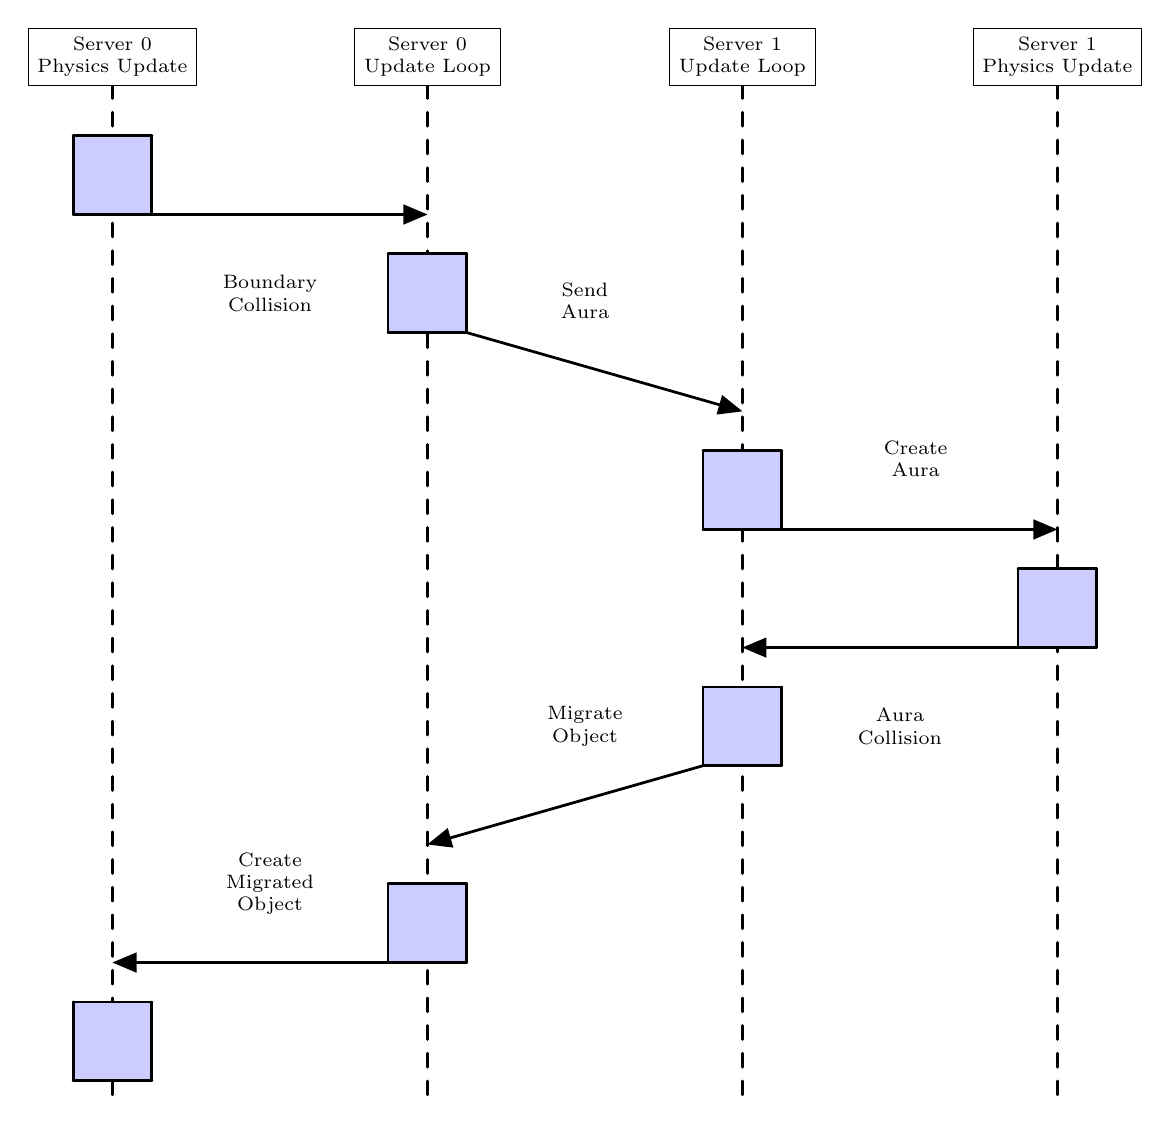
\begin{tikzpicture}[line cap=round,line join=round,>=triangle 45,x=1cm,y=1cm,every node/.style={font=\scriptsize,
		minimum height=0.25cm,minimum width=0.5cm},,scale=1.0]

\draw [line width=1pt,dash pattern=on 5pt off 5pt] (-2.0,6)-- (-2.0,-7.25);
\draw [line width=1pt,dash pattern=on 5pt off 5pt] (2.0,6)-- (2.0,-7.25);
\draw [line width=1pt,dash pattern=on 5pt off 5pt] (6.0,6.0)-- (6.0,-7.25);
\draw [line width=1pt,dash pattern=on 5pt off 5pt] (-6.0,6)-- (-6.0,-7.25);
\draw [->,line width=1pt] (-5.5,4) -- (-2.0,4);
\draw [->,line width=1pt] (-1.5,2.5) -- (2.0,1.5);
\draw [->,line width=1pt] (2.5,0) -- (6.0,0);
\draw [->,line width=1pt] (5.5,-1.5) -- (2.0,-1.5);
\draw [->,line width=1pt] (1.5,-3) -- (-2.0,-4);
\draw [->,line width=1pt] (-2.5,-5.5) -- (-6.0,-5.5);
\fill[line width=2pt,color=blue!20] (-6.5,5) -- (-6.5,4) -- (-5.5,4) -- (-5.5,5) -- cycle;
\fill[line width=2pt,color=blue!20] (-2.5,3.5) -- (-2.5,2.5) -- (-1.5,2.5) -- (-1.5,3.5) -- cycle;
\fill[line width=2pt,color=blue!20] (1.5,1) -- (1.5,0) -- (2.5,0) -- (2.5,1) -- cycle;
\fill[line width=2pt,color=blue!20] (5.5,-0.5) -- (5.5,-1.5) -- (6.5,-1.5) -- (6.5,-0.5) -- cycle;
\fill[line width=2pt,color=blue!20] (1.5,-2) -- (1.5,-3) -- (2.5,-3) -- (2.5,-2) -- cycle;
\fill[line width=2pt,color=blue!20] (-2.5,-4.5) -- (-2.5,-5.5) -- (-1.5,-5.5) -- (-1.5,-4.5) -- cycle;
\fill[line width=2pt,color=blue!20] (-6.5,-6) -- (-6.5,-7) -- (-5.5,-7) -- (-5.5,-6) -- cycle;
\draw [line width=1pt] (-6.5,5)-- (-6.5,4);
\draw [line width=1pt] (-6.5,4)-- (-5.5,4);
\draw [line width=1pt] (-5.5,4)-- (-5.5,5);
\draw [line width=1pt] (-5.5,5)-- (-6.5,5);
\draw [line width=1pt] (-2.5,3.5)-- (-2.5,2.5);
\draw [line width=1pt] (-2.5,2.5)-- (-1.5,2.5);
\draw [line width=1pt] (-1.5,2.5)-- (-1.5,3.5);
\draw [line width=1pt] (-1.5,3.5)-- (-2.5,3.5);
\draw [line width=1pt] (1.5,1)-- (1.5,0);
\draw [line width=1pt] (1.5,0)-- (2.5,0);
\draw [line width=1pt] (2.5,0)-- (2.5,1);
\draw [line width=1pt] (2.5,1)-- (1.5,1);
\draw [line width=1pt] (5.5,-0.5)-- (5.5,-1.5);
\draw [line width=1pt] (5.5,-1.5)-- (6.5,-1.5);
\draw [line width=1pt] (6.5,-1.5)-- (6.5,-0.5);
\draw [line width=1pt] (6.5,-0.5)-- (5.5,-0.5);
\draw [line width=1pt] (1.5,-2)-- (1.5,-3);
\draw [line width=1pt] (1.5,-3)-- (2.5,-3);
\draw [line width=1pt] (2.5,-3)-- (2.5,-2);
\draw [line width=1pt] (2.5,-2)-- (1.5,-2);
\draw [line width=1pt] (-2.5,-4.5)-- (-2.5,-5.5);
\draw [line width=1pt] (-2.5,-5.5)-- (-1.5,-5.5);
\draw [line width=1pt] (-1.5,-5.5)-- (-1.5,-4.5);
\draw [line width=1pt] (-1.5,-4.5)-- (-2.5,-4.5);
\draw [line width=1pt] (-6.5,-6)-- (-6.5,-7);
\draw [line width=1pt] (-6.5,-7)-- (-5.5,-7);
\draw [line width=1pt] (-5.5,-7)-- (-5.5,-6);
\draw [line width=1pt] (-5.5,-6)-- (-6.5,-6);
\draw[color=black,align=center] (-4,3.0) node {Boundary\\Collision};
\draw[color=black,align=center] (4.2,0.9) node {Create\\Aura};
\draw[color=black,align=center] (0.0,2.9) node {Send\\Aura};
\draw[color=black,align=center] (4.0,-2.5) node {Aura\\Collision};
\draw[color=black,align=center] (-0.0,-2.5) node {Migrate\\Object};
\draw[color=black,align=center] (-4.0,-4.5) node {Create\\Migrated\\Object};

\draw (-6,6) node[draw,anchor=center,align=center,fill=white] {Server 0\\Physics Update};
\draw (-2,6) node[draw,anchor=center,align=center,fill=white] {Server 0\\Update Loop};
\draw (6,6) node[draw,anchor=center,align=center,fill=white] {Server 1\\Physics Update};
\draw (2,6) node[draw,anchor=center,align=center,fill=white] {Server 1\\Update Loop};
\end{tikzpicture}
	\caption{Aura and migration sequence diagram}
	\label{sequence_diagram}
\end{figure}

\section{Sub-optimal object hosting}
As objects within each others auras need to be simulated on the same server, this can lead to objects being deep within another server's region (objects that are far from the region boundary).

Clusters of objects can therefore end up being simulated with all but one of their objects in their host server's region. This is sub-optimal, as the more auras that are being maintained/exchanged, the higher the computational cost.

The solution to this problem is to dynamically move the server-region boundaries to prevent clusters of objects having the majority of the objects outside of their host server region or the server-region boundaries could be moved in such a way as to avoid intersecting large clusters of objects entirely. However, this solution is not yet implemented in AP.

\section{Thrashing}\label{Thrashing}
The common term `thrashing' will be used to describe the following two scenarios that must be considered.

1. 3-Object Thrashing - An object may be overlapping two auras from different servers. Given appropriate velocity, this could result in object migration, followed by aura collision, followed by migration and then repeating the process again. For example, Objects K, L and M in Fig. \ref{AuraProj}. Object K lies inside the auras of both Object L and M. 

In order to prevent this thrashing, when an object is migrated, it is also migrated with any objects found that lie within the aura of the object or have an existing aura which overlaps the migrating object's aura. This is carried out recursively to ensure all objects that are overlapping are migrated at the same time.

2. 2-Object Thrashing - Two objects on different servers may both trigger the migration of the other. For example, Objects C and D in Fig. \ref{AuraProj}. Suppose the two objects are moving towards each other. Object C collides with the aura of object D and begins migrating to Server 1. Before Object C is received (and the message processed), object D collides with the aura of Object C and begins migrating to Server 0. The two objects remain on different servers and the process can repeat again, indefinitely.

When Object C is received, the object is created in Server 0's physics simulation and the aura for that object is removed from Server 0's physics simulation. 
The next physics time-step on Server 0, the object is within the aura distance of the boundary with Server 1, a message for the aura of object C will added to the send buffer for Server 1. The next network update, the message will be sent to Server 1.
If Object C intersects an aura from Server 1, in this case Object D's aura, it will be added to the object send buffer for Server 1. The next network update, the message will be sent to Server 1. %And the aura no longer sent?
The message for Object C's aura is received by Server 1 and processed on the next network update, when processed, a trigger volume for Object C's aura will be created in the physics engine of Server 1. The next physics time-step on Server 1, any objects within that aura will call a trigger callback, in this case Object D, indicating that object D has collided with an aura and so should be migrated to Server 0. Object D is added to the object send buffer for Server 0 and the next network update, Object D is migrated.

%TODO: Check if aura sent in addition to the object migration? Yes, but it is also sent with an aura remove message
%TODO: Check if aura removed immediately when object is received? Will be received at the same time as the aura remove message, which will remove the aura immediately
%TODO: WIll the immediately remove aura still trigger a callback? It shouldn't do, as it checks for removed shapes


In order for this process to repeat, both objects must have their migrations triggered (during a physics update) before the message of the other object migration has been received and processed and a physics time step has occurred to remove the aura trigger volume from the physics simulation.

In order for this to occur, each object must have its aura created (first physics time step after arrival) before the aura of the other object or the other object itself has been received (if the aura is received, it will trigger the migration immediately, so an aura will not be sent, if the other object is received, the aura will be removed). Each object has its aura received by the other server, triggering the migration of the other object. The cycle is broken once an object is received and its aura removed before the other object has its migration triggered when a physics time step occurs.

%Proposed solution 1: If an object collides with an aura that has just been created (was created in the most recent physics time step), only migrate the object if the colliding object id is greater (or lower than) the object projecting the aura's id. This will allow a physics time step to occur and the aura removed, if the object projecting the aura is being migrated. Should work so long as the migration message is received and processed on the waiting server before its next physics time step, i.e. round-trip time is less than two physics time steps. Aura is sent on step 0, remote aura is received, it gets created in step 1 and ignored for the first step of existense, the migrate message is received and the aura is removed in step 2

%Proposed solution 2: If an object collides with another object's aura and is also projecting an aura they will both be colliding with each other's aura (if the two objects have identical rotations or are spheres). If an object knows the other object is colliding/will collide with its aura, only migrate if object id is higher or lower or rank of server is higher or lower. Would rely on knowing the exact shape of the collider of the other object

\section{Islands}
When an object traverses a region boundary, the object is migrated only if it does not overlap an aura projected by an object from the same server. In the context of migrations, an island is defined as two or more objects located outside of their host server's region (i.e. have traversed a region boundary) but are each within the aura projected from objects owned by the same host. For example, Objects H, I, and J illustrated in Fig. \ref{AuraProj}. No objects in the island are migrated as each object is within the aura of another object in the island. This should be prevented as it causes processing and networking overhead and is unnecessary as all objects lie within the region of Server 2 and are not interacting with any other objects from Server 0. 

To prevent islands, a search is performed at each time step to determine if an object is part of an island. A search is performed to determine if a potential migratory object is within a group of objects with overlapping auras, of which none are positioned within the hosting server region. If the group of objects has no members within the hosting server region then the object is part of an island and the entire island of objects is migrated. Otherwise, no action is taken. For example, in Fig. \ref{AuraProj} Object I has overlapping auras with Objects H and J. H and J are checked for overlap with the Server 0 - Server 1 region boundary and for overlap with auras from Server 0 that are intersecting the Server 0 - Server 1 boundary. In this scenario, H and J are found to be part of an island, so H, I, and J are all migrated to Server 2. If objects are found to not be part of an island, no action is taken. For example, Objects E, F, and G in Fig. \ref{AuraProj}. Object F is found to have an overlapping aura with Object E, but Object E intersects the Server 0 - Server 1 boundary, so E, F, and G are found to not be part of an island and therefore no action is taken. This solution is shown in Algorithm \ref{boundaryAlgorithm} and the problem of islands can therefore be considered solved.

\section{Corner Case}\label{CornerCase}
This section discusses how AP handles corner cases, i.e., where the boundary of more than two servers meet. 

An example of the corner case is illustrated in Fig. \ref{AuraProj}. Object N, hosted on Server 2, sends an aura to Server 0. Object O, on Server 1, sends an aura to Server 0. Object N's aura overlaps with Object O's on server 0. Server 2 is unaware of Object O and Server 1 is unaware of Object N. As the two auras overlap, there is a potential interaction between the objects, yet the two objects remain on separate servers. To solve this problem, auras from boundaries between two neighbouring servers are shared. In the region layout in Fig. \ref{AuraProj}, auras from a boundary are received by interested servers. In the Object N and O example, Server 2 would send Object N's aura to Server 1; when Object O collides with Object N's aura, migration to Server 2 occurs.

A server has to receive the auras of all objects from neighbouring boundaries, as objects being simulated by a server can exist anywhere in a neighbouring server's region. Our assumption is that a region a server simulates is sufficiently large enough to prevent the aura overlap of objects from non-neighbouring servers.

\section{Benefits of Proposed Solution}
Aura Projection has the following benefits over other considered solutions. AP guarantees strong consistency of collisions, meaning diverging results on different servers are prevented. Objects are only simulated once on a one server, instead of being simulated on multiple servers, requiring more computation time per object. No synchronisation is required between servers, as each server is running an entirely autonomous simulation, there is no need for any synchronisation to take place between servers.

\section{Limits of Proposed Solution}
Performance of the system will be measured using the highest cost across all servers, this will be referred to as $costmax$. If the addition of one or more servers (and/or re-partitioning of servers) cannot be done without causing a higher $costmax$, the system cannot be scaled up further.

It is possible to predict whether or not a new configuration has a higher or lower $costmax$ using the following process. Let B:N be the performance cost ratio of boundary to non-boundary objects (this cost ratio will differ for different simulations and may either be a constant ratio or a function, but we will assume it is a constant for this estimate). Due to boundary objects having additional processing and networking overhead, we can assume the B:N ratio will always be greater than 1. The performance cost can then be estimated for each server in the new configuration by summing the boundary and non-boundary objects and using the B:N cost estimate. If this results in a lower $costmax$ the performance of the system will be increased.

Let $cost(x)$ be the performance cost of a server x.
Let $Obj_{bdry}$ and $Obj_{nonbdry}$ be the number of boundary and non-boundary objects respectively for a given server x.

\begin{equation}
	cost(x) = (Obj_{bdry}\cdot B:N) + Obj_{nonbdry}
\end{equation}

Let N be the number of servers. The $cost_max$ of a server can be calculated using the following equation:
\begin{equation}
	costmax = max(cost(1),...,cost(N))
\end{equation}

Let $costmax_n$ be the current $costmax$ of system and $costmax_{n+1}$ be the $costmax$ of a potential new configuration.

\begin{equation}
	costmax_{n+1} < costmax_n
\end{equation}

The $costmax_{n+1}$ must be less than $costmax_n$ in order for a performance gain to occur. If no possible $costmax_{n+1}$ with a lower value exists, the overall performance of the system cannot be increased and the system will have reached the limit of scalability.

Example 1:
Let 1 non-boundary object have the cost value of 1 and suppose the B:N ratio is a constant 2:1.
1 server with 1000 non-boundary objects. The $costmax_n$ is 1000. 1 server is added, the simulation is partitioned so that 500 non-boundary objects exist on each. The $costmax_{n+1}$ is 500. 500<1000, so new configuration results in better performance.

Example 2:
2 servers with 1000 non-boundary objects each. The $costmax_n$ is 1000. 1 server is added, the simulation, the best partitioning that can be achieved results in 1 server having 250 non-boundary and 400 boundary objects. The $costmax_{n+1}$ is (400*B:N)+250 = 1050. 1050>1000, so the new configuration results in worse performance. As this is the best partitioning that could be achieved the system cannot be scaled up further.

Using the logic above and the assumptions made, it can be deduced that the main limiting factor of Aura Projection is the number of unavoidable boundary objects present on a single server in the simulation.

\section{Problem Definition Summary}
In this chapter, the following points have been addressed:
\begin{itemize}
	\item The requirements of a solution to scalable real-time physics.
	\item The challenges of distributing a real-time physics engine and potential solutions.
	\item A description and justification of AP, including the aura calculation.
	\item The implemented solutions to the problems of: 3-object thrashing; islands; and the corner case.
	\item The proposed solutions to: sub-optimal object hosting and 2-object thrashing, which are not yet implemented.
\end{itemize}

\chapter{Implementation}
This section will discuss an implementation of AP using PhysX and RakNet.

%TODO: Mention and justify update rate and tick-rate are the same for these experiments for the sake of simplicity.

\section{System Architecture}
The simulation space is partitioned into regions, with each region consisting of its own instance of PhysX running on a dedicated GPU-enabled machine in the cloud. The boundary between regions is defined as a vertical plane, two-dimensionally dividing the simulation space into one region per server. The network library RakNet is used for all message passing between servers. RakNet ensures messages exhibit best effort and are received in sent order.

When objects project auras they are added to a send aura buffer that is sent to all servers associated to the boundary of concern. Each object has a unique identifier (ID). When an aura is received by a server, an aura is created if it does not already exist, otherwise the aura is updated using the data received. When an object is no longer projecting its aura, the ID of that object is added to the delete buffer which is then sent to all servers neighbouring the boundary.

When objects traverse region boundaries, they are added to a migration buffer with all information required to duplicate an object at a neighbouring server. The contents of a migration buffer are sent to a server now responsible for hosting an object. When migration messages are received an object is created within the server's simulation.
% ^^^^ Replace 'an' with 'each'?

Clients may connect to any server and are provided with a streamed visualisation of the simulation in real-time. Clients may also interact with and influence the simulation, providing a comprehensive solution for real-time interactive physics. The client system was built using the Unreal Engine. Once a client is connected, the position and states (replicas) of all objects in the simulation are sent from each server to the client via the RakNet Replica Manager.

\begin{figure}[!t]
	\centering
	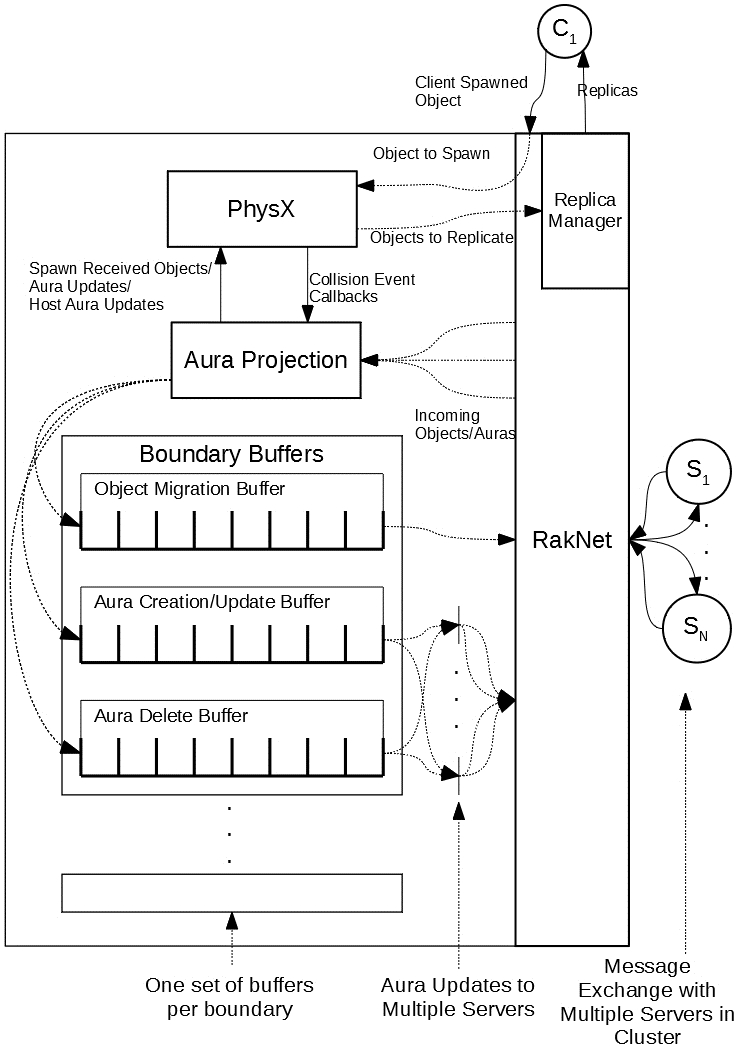
\includegraphics[width=\textwidth]{ArchitectureDiagramVertical}
	\caption{Server Architecture}
	\label{fig_stack}
\end{figure}

\section{Algorithms}
$AC$ is called when an object collides with an aura. A recursive search is performed in order to find all objects that would lie within each object's aura, preventing thrashing as discussed in \ref{Thrashing}. Once the recursive search is complete, all objects are added to the send buffer.

\renewcommand{\algorithmicforall}{\textbf{for each}}
\algnewcommand{\LeftComment}[1]{\State \(\triangleright\) #1}
\algnewcommand\And{\textbf{and}}
\algnewcommand\Or{\textbf{or}}

\begin{algorithm}
	\caption{Object Migrate - Aura Collision ($AC$)}\label{auraAlgorithm}
	\begin{algorithmic}[1]
		\Procedure{OnAuraEnter}{}	\Comment{A callback on an object}
		\LeftComment{Track visited objects to prevent infinite recursion}
		\State $\textit{visited := \{\}}$
		\LeftComment{Recursively send object with objects that would lie within each object's aura}
		\State \Call{SendWithOverlaps}{$\textit{thisObject, visited}$}
		\EndProcedure
		\State
		\Procedure{SendWithOverlaps}{$\textit{object, visited}$}
		\LeftComment{Get objects whose auras overlap this object's aura} %using a $\mathcal{O}(n)$ scene query
		\State $\textit{overlaps :=}$ \Call{GetAuraOverlaps}{$\textit{object}$} %\Comment{$\mathcal{O}(n)$ scene query}
		\State
		\ForAll{{$\textit{object} \in \textit{overlaps}$}} :
		\If {$\textit{object} \not \in \textit{visited}$}:
		\State $\textit{visited := visited + object}$
		\State \Call{SendWithOverlaps}{$\textit{object, visited}$}
		\EndIf
		\EndFor
		\State
		\State\Call{AddToSendBuffer}{object}
		\EndProcedure
	\end{algorithmic}
\end{algorithm}

$BT$ is called when an object traverses a boundary. In order to prevent `islands' forming (for example Objects H, I and J in Fig. \ref{AuraProj}), a recursive search is carried out to determine is an object is part of an island or not. If an object is found to not be part of an island, the entire cluster of objects is added to the send buffer, otherwise no action is taken.

\begin{algorithm}
	\caption{Object Migrate - Boundary Traverse ($BT$)}\label{boundaryAlgorithm}
	\begin{algorithmic}[1]	
		\LeftComment{Update called on each boundary}
		\Procedure{BoundaryUpdate}{}
		\State $\textit{checked := \{\}}$	\Comment{Used to prevent duplicate checks}
		\State
		\LeftComment{Loop over fully traversed objects from latest update}
		\ForAll{{$\textit{object} \in \textit{traversed}$}} : 
		%\If {$\textit{object.isSleeping} = \textit{false} \And \textit{object} \not \in \textit{checked}$}:
		\If {$\textit{object} \in \textit{checked}$}:
		\State $\textit{continue}$
		\EndIf
		
		\State $\textit{island := \{\}}$
		\State $\textit{isIsland := }\Call{IslandQuery}{\textit{object, island}}$
		\LeftComment{IslandQuery() returns true if object is part of an island and a list of objects in the island}
		\If {$\textit{isIsland} = \textit{true}$}:
		\State \Call{SendGroup}{$\textit{island}$}
		\EndIf
		\State $\textit{checked := checked + island}$
		\EndFor
		%		\State $\textit{visited := \{\}}$	\Comment{Track visited to prevent infinite recursion}
		%		\State \Call{SendWithOverlaps}{$\textit{thisObject, visited}$}
		\EndProcedure
		\State
		\Function{IslandQuery}{$\textit{object, visited}$}
		\State $\textit{visited := visited + object}$
		\If {$\textit{object.overlapsHostRegion = true}$}
		\State return $\textit{false}$
		\EndIf
		%\If {$\textit{object.boundaryCollisionCount = 0}$}
		%\State return $\textit{false}$
		%\EndIf
		\State
		\LeftComment{Get objects whose auras overlap this object's aura} %using a $\mathcal{O}(n)$ scene query
		\State $\textit{overlaps :=}$ \Call{GetMutalAuraOverlaps}{$\textit{object}$}
		\State
		\LeftComment{If all objects with overlapping auras are islands, then this object is an island}
		\State $\textit{isIsland := true}$
		\ForAll{{$\textit{object} \in \textit{overlaps}$}} :
		\If {$\textit{object} \not \in \textit{visited}$}:
		\State $\textit{isIsland \&= }$ \Call{IslandQuery}{$\textit{object,visited}$}
		\EndIf
		\EndFor
		\State return $\textit{isIsland}$
		\EndFunction
		%		
		%		\Procedure{SendWithOverlaps}{$\textit{object, visited}$}
		%		\State $\textit{overlaps :=}$ \Call{GetOverlaps}{$\textit{object}$} \Comment{$\mathcal{O}(n)$ scene query}
		%		\ForAll{{$\textit{object} \in \textit{overlaps}$}} :
		%		\If {$\textit{object} \not \in \textit{visited}$}:
		%		\State $\textit{visited := visited + object}$
		%		\State \Call{SendWithOverlaps}{$\textit{object, visited}$}
		%		\EndIf
		%		\EndFor
		%		
		%		\State\Call{Send}{object}
		%		\EndProcedure
	\end{algorithmic}
\end{algorithm}

$OBC$ is called when an object collides with a boundary. The object's aura is calculated and added to the boundary's send aura buffer. A host aura is also created, to allow for the checking of mutual aura overlaps and prevent thrashing, if this is the first boundary intersection.

\begin{algorithm}
	\caption{Create Aura - Object boundary collision ($OBC$)}\label{createAuraBoundaryAlgorithm}
	\begin{algorithmic}[1]
		\LeftComment{A callback on an object, called when an object collides with a boundary}
		\Procedure{OnBoundaryEnter}{$\textit{boundary}$}
		\State \Call{AddToAuraBuffer}{$\textit{boundary, this}$}
		\State
		\LeftComment{Create `host aura' so GetMutalAuraOverlaps() will detect this object's aura}
		\If {$\textit{boundaryIntersections = 0}$}
		\State \Call{CreateHostAura}{$\textit{}$}
		\EndIf
		\State $\textit{boundaryIntersections := boundaryIntersections + 1}$
		%\State $\textit{boundariesEntered := boundariesEntered + boundary}$
		%	\State $\textit{boundary->addToOverlappingOtherObjects(m_rigidDynamic)}$
		%	\State $\textit{boundary->addBoundaryBodyToSendBuffer(this)}$
		\EndProcedure
	\end{algorithmic}
\end{algorithm}

$OBU$ is called once per frame that an object is intersecting a boundary. If the object is not `sleeping', a new aura is calculated and added to the boundary's send buffer and the host aura is updated.

The isSleeping() function returns true if an object is sleeping. From the PhysX documentation:
An object is considered `sleeping' when an actor does not move for a period of time. (The default PhysX period of time is $0.4s$ and this is the value used in our approach). Objects are `woken up' when they are touched by an awake object. 

\begin{algorithm}
	\caption{Update Aura - Object boundary update ($OBU$)}\label{objectWithAuraAlgorithm}
	\begin{algorithmic}[1]
		\LeftComment{A callback on an object, called per step per boundary the object is colliding with}
		\Procedure{onBoundaryUpdate}{$\textit{boundary}$}
		\If {$\textit{this.isSleeping = true}$}
		\State $\textit{return}$
		\EndIf
		\LeftComment{Send Aura Delta}
		\State \Call{AddToAuraBuffer}{$\textit{boundary, this}$} 
		\State \Call{UpdateHostAura}{$\textit{}$}
		%		if (!m_hasBeenSent 
		%	&& (m_app->isBoundaryOtherActor(triggerPair.triggerActor))
		%	&& !m_rigidDynamic->isSleeping()
		%	&& !m_rigidDynamic->getAngularVelocity().isZero()
		%	&& !m_rigidDynamic->getLinearVelocity().isZero()
		%	)
		%	{
		%		OrionBoundaryOther* boundary = (OrionBoundaryOther*)triggerPair.triggerActor->userData;
		%		boundary->addBoundaryBodyToSendBuffer(this);
		%	}
		%	
		%	if (m_app->isBoundaryOtherActor(triggerPair.triggerActor))
		%	{
		%		updateBoundingBox();
		%	}
		\EndProcedure
	\end{algorithmic}
\end{algorithm}

$OBE$ is called when an object is no longer intersecting a boundary. The object is added to the boundary's remove aura buffer. If the object is no longer intersecting any boundaries, the host aura is deleted.

\begin{algorithm}
	\caption{Destroy Aura - Object boundary exit ($OBE$)}\label{destroyAuraAlgorithm}
	\begin{algorithmic}[1]
		\LeftComment{A callback on an object, called when an object exits a boundary}
		\Procedure{onBoundaryExit}{$\textit{boundary}$}
		\State \Call{AddtoDeleteAuraBuffer}{$\textit{}$}
		\State
		\LeftComment{If object is no longer sending an aura, no need to keep a `host aura'}
		\State $\textit{boundaryIntersections := boundaryIntersections - 1}$
		\If {$\textit{boundaryIntersections = 0}$}
		\State \Call{DeleteHostAura}{$\textit{}$}
		\EndIf
		
		%	// If leaving boundary of other simulation, send message removing object from other boundary triggers
		%	if (!m_hasBeenSent && m_app->isBoundaryOtherActor(triggerPair.triggerActor))
		%	{
		%		OrionBoundaryOther* boundary = (OrionBoundaryOther*)triggerPair.triggerActor->userData;
		%		vector<OrionBoundaryOther*>::iterator found = find(m_boundariesWithAuras.begin(), m_boundariesWithAuras.end(), boundary);
		%		if (found != m_boundariesWithAuras.end())
		%		{
		%			boundary->addBoundaryBodyRemoveToSendBuffer(m_index);
		%			boundary->removeFromOverlappingOtherObjects(m_rigidDynamic);
		%			m_boundariesWithAuras.erase(find(m_boundariesWithAuras.begin(), m_boundariesWithAuras.end(), boundary));
		%		}
		%	}
		%	
		%	if (m_app->isBoundaryOtherActor(triggerPair.triggerActor))
		%	{
		%		m_partiallyInsideOtherCount--;
		%		PX_ASSERT(m_partiallyInsideOtherCount >= 0);
		%		if (m_partiallyInsideOtherCount == 0)
		%		{
		%			deleteBoundingBox();
		%		}
		%	}
		\EndProcedure
	\end{algorithmic}
\end{algorithm}

$BNU$ is called once per network connection between servers. It is responsible for sending and receiving object migrations and auras between servers, including the sending and receiving of auras from boundaries between other neighbouring remote servers.

\begin{algorithm}
	\caption{Boundary Network Update ($BNU$)}\label{boundaryNetworkAlgorithm}
	\begin{algorithmic}[1]
		\LeftComment{Update called once per network connection}
		\Procedure{Network Update}{}
		\LeftComment{Exchange migrations with target server}
		\State \Call{SendObjectsInBuffer}{}
		\State \Call{ReceiveObjects}{}
		\State
		\LeftComment{Send aura state updates to all neighbours}
		\ForAll{{$\textit{neighbour} \in \textit{neighbours}$}} :
		\State \Call{SendAurasInBuffer}{}
		\State \Call{SendDeleteAurasInBuffer}{}
		\State \Call{ReceiveAuras}{}
		\State \Call{ReceiveDeleteAuras}{}
		\EndFor
		%	sendRigidDynamics();
		%recvRigidDynamicUpdate();
		%
		%vector<OrionAuraExchangeBoundary*>::const_iterator it;
		%for (it = m_auraExchange.begin(); it != m_auraExchange.end(); ++it)
		%{
		%	sendBoundaryBodies(*it);
		%	sendBoundaryBodiesRemove(*it);
		%	recvBoundaryBodyUpdate(*it);
		%	recvBoundaryBodyRemoveUpdate(*it);
		%}
		\EndProcedure
	\end{algorithmic}
\end{algorithm}

\begin{figure}[hbt]
	\centering
	\resizebox{\columnwidth}{!}{
		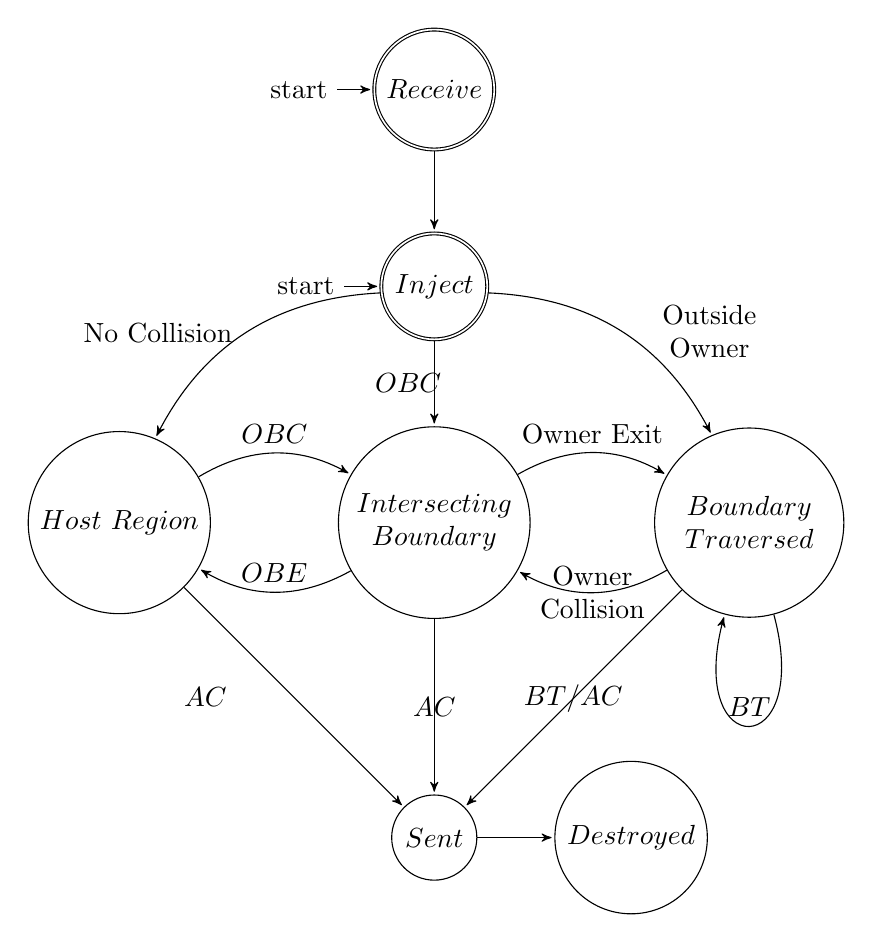
\begin{tikzpicture}[>=stealth',shorten >=1pt,auto,node distance=2.5cm]
		\node[initial,state,accepting,align=center] (R) {$Receive$};
		\node[initial,state,accepting] (S) [below of=R] {$Inject$};
		\node[state]         (q2) [below of=S, node distance=3cm, text width=2cm, align=center] {$Intersecting$ $Boundary$};
		\node[state]         (q1) [left of=q2, node distance=4cm]  {$Host$ $Region$};
		\node[state]         (q3) [right of=q2, node distance=4cm, text width=2cm, align=center] {$Boundary$ $Traversed$};
		\node[state]         (q4) [below of=q2, node distance=4cm] {$Sent$};
		\node[state]         (q5) [right of=q4] {$Destroyed$};
		
		
		\path[->] 
		(R) edge node {} (S)
		(S) edge [bend right] node [left, text width=2cm, align=center] {No Collision} (q1)
		(S) edge node [anchor=center, text width=1.5cm, align=left] {$OBC$} (q2)
		(S) edge [bend left] node [right, text width=2cm, align=center] {Outside Owner} (q3)
		%(q1) edge [loop above] node {} (q1)
		%(q2) edge [loop left] node {} (q2)
		(q3) edge [loop below] node [above] {$BT$} (q3)
		(q1) edge node [left, text width=2cm, align=center] {$AC$} (q4)
		(q2) edge node [anchor=center, text width=2cm, align=center] {$AC$} (q4)
		(q3) edge node [anchor=center, text width=2cm, align=center] {$BT$/$AC$} (q4)
		
		(q1) edge [bend left] node [anchor=center, text width=1.5cm, align=center, above] {$OBC$} (q2)
		(q2) edge [bend left] node [anchor=center, text width=2cm, align=center, above] {$OBE$} (q1)
		(q3) edge [bend left] node [anchor=center, text width=2cm, align=center] {Owner Collision} (q2)
		(q2) edge [bend left] node [anchor=center, above, text width=2cm, align=center] {Owner Exit} (q3)
		
		(q4) edge node {} (q5)
		
		%(S)  edge [loop above] node {a} (S)
		%edge              node {a} (q1)
		%(q1) edge [bend left]  node {a} (S)
		%edge              node {b} (q2)
		%(q2) edge [loop above] node {b} (q2)
		%edge [bend left]  node {b} (q1)
		;
		\end{tikzpicture}
	}
\end{figure}

\section{The Visualiser}
%We discuss the features and implementation of the visualiser, including server and client created replicas, static objects and interactivity. The challenges of multiple servers are explained and our solutions justified. Screenshots from demo scenes have been included.
We will now discuss the details of the visualiser, both the features and implementation details.

The visualiser is built using Unreal Engine and the RakNet plugin.

\begin{figure}[!t]
	\centering
	\includegraphics[width=\textwidth]{Blocks}
	\caption{Stacks of objects near and on a corner boundary. This demo scene consists of two large stacks of server created cuboid replicas near the corner of four server regions. Either side of each server boundary are random injection volumes, in which server created objects are injected into the simulation, randomly, within a volume. Each colour represents a different owning server.}
	\label{fig_screen1}
\end{figure}

\begin{figure}[!t]
	\centering
	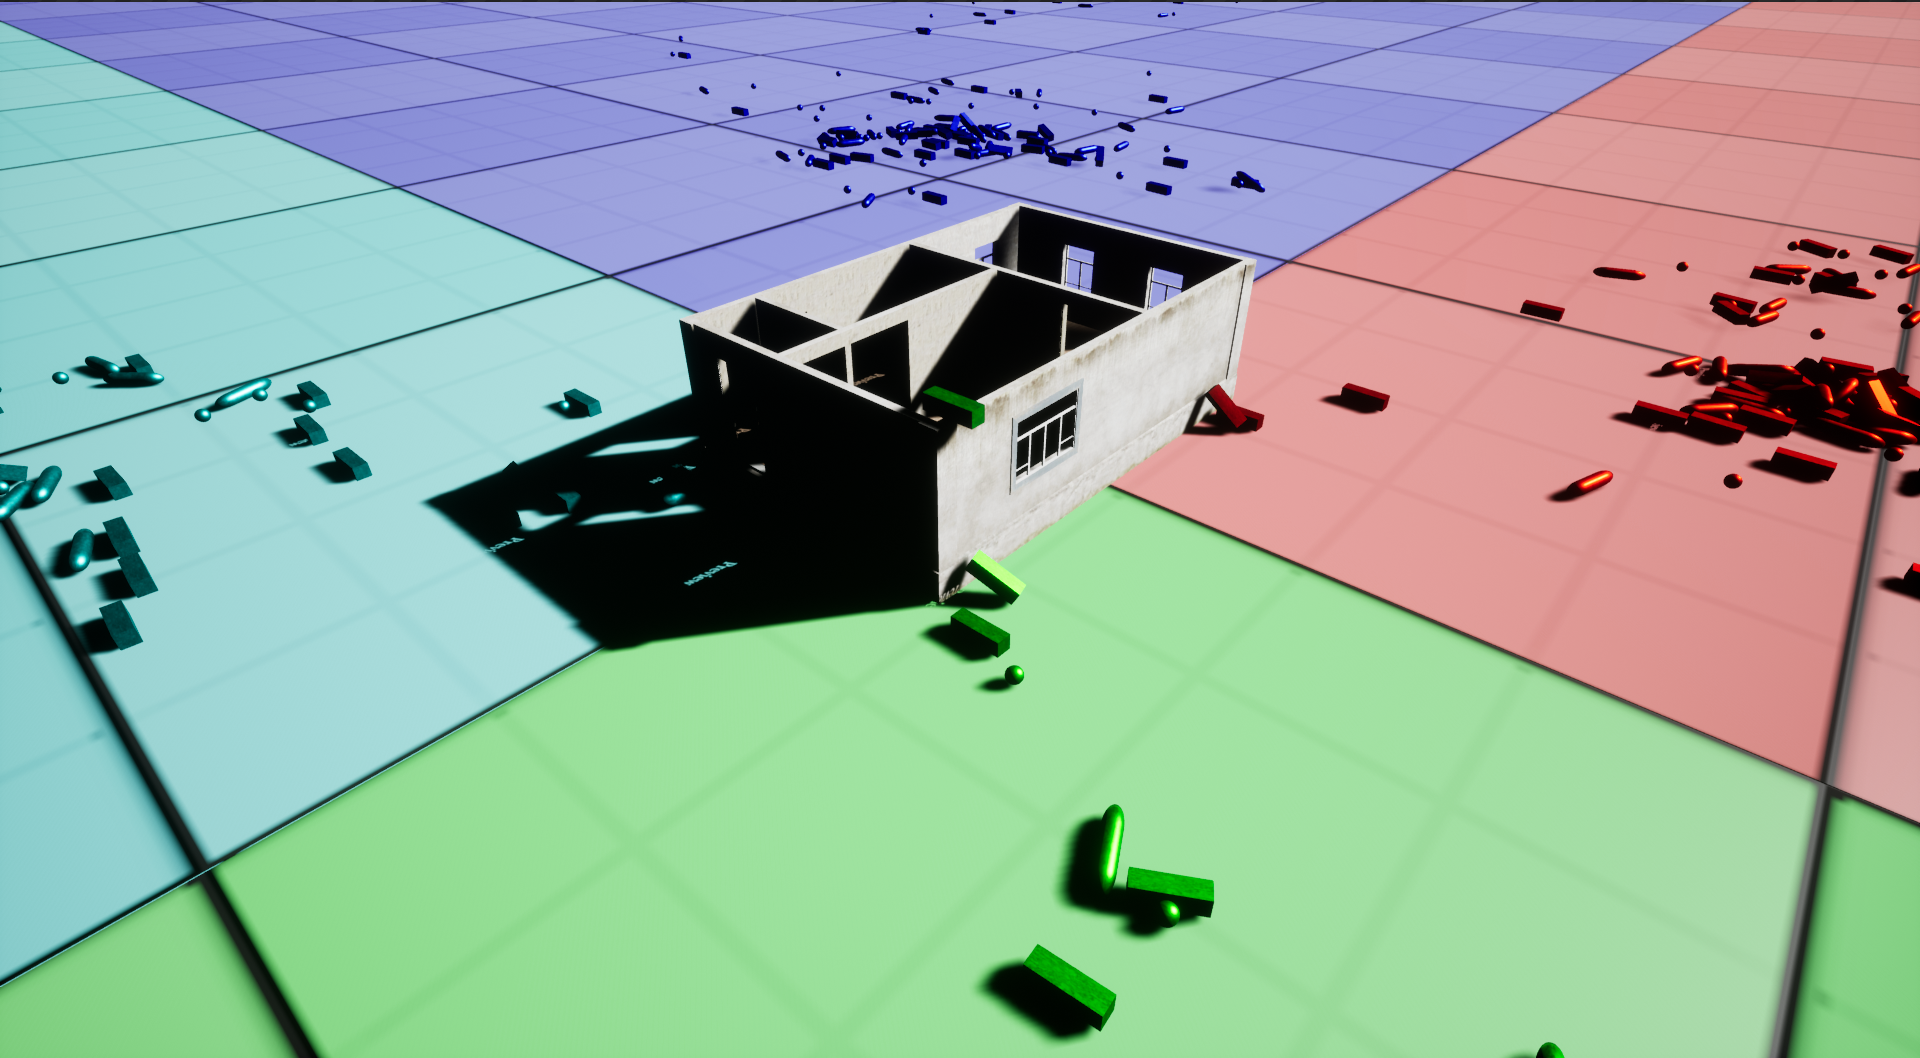
\includegraphics[width=\textwidth]{screenshot}
	\caption{A static object on a corner boundary surrounded by objects being simulated on different servers. This demo scene includes a client-created static object (a building), which is being simulated on all servers. Numerous server created objects surround the building, which have been triggered from within the client.}
	\label{fig_screen2}
\end{figure}

The visualiser connects to multiple servers, objects are simulated on server and those objects from all servers are replicated on the visualiser. These are referred to as replica objects. The visualiser uses RakNet's ReplicaManager, which is responsible for: the creation of replicas objects on both the server and client; communicating the state of objects from the server to the client, in order for the replica objects to be replicated; and the deletion of replica objects. Replica objects are replicated on the visualiser by the server sending the state (position, rotation) to the client, the replica representation on the client is then updated with the newly received state from the server. The object state is optimised to reduce processing and network overhead, by only sending updates of the position and rotation to the client, when they change on the server.

Replica objects can be created in one of two ways. Either by the server or by the client. We will now discuss the implementation details of each type of replica creation.

The visualiser supports server-created replica objects, which are limited to pre-defined basic objects (cuboid, sphere \& capsule). A different render material per server is used to identify the owning server of each object. These server objects have pre-defined representations on the client. The server sends an identifier for the type of object, which is then created on the client. Using pre-defined objects means the whole geometry of the object does not need to be transferred to the client. This is useful for when there are a large number of identical objects as it avoids having to re-send the same geometry for each object. However, this method requires the client to know of these pre-defined types.

The visualiser also supports arbitrary client-created objects. Entire scenes can be created in the client at edit-time, in the Unreal Engine Editor, and then re-created on servers when connections to the servers are made. This works for objects with any mesh, i.e. the server does not need to know about the geometry of an object when the server is built and deployed, the client communicates all data required to create the physical object on the server. All objects marked for replication on the servers are sent to all servers, if an object exists outside of a server's region, the creation is skipped, meaning the replica object is created only on the server containing the replica object. The central point of the object is used, avoiding conflicts between servers when an object exists that intersects a server region boundary.

In addition to replica objects, static object can also be created by the client. As these objects are static, there is no need for their states to be replicated as they do not change over the course of the simulation. Static object work simply by the client sending the geometry, position and rotation details of the static object to all servers and the servers then re-create the static object. These static objects then remain unchanged throughout the simulation, requiring no updates to the state to be communicated to the client. Static objects are created on all servers, this could be optimised so only static objects within a server's region are created, however, AP can lead to clusters of objects being simulated outside of their host server's region, which may interact with static objects that do not exist on their host server. In addition, the cost of simulating static objects tends to be very low, as they do not require any updates as they are not dynamic. In the future, region boundaries may change; a server may become responsible for a static object previously residing in another server's region, which would then have to be communicated when the region boundaries changed, by all servers simulating all static objects, this avoids the need for extra communication when server boundaries change. With these trade-offs in mind, we have elected to create all static objects on all servers, when static objects are used in a simulation.

The visualiser also allows for interactivity, the creation of server-created objects can be triggered from the client, as well as allowing the user to reset or change scenes that are being simulated on the server.

Currently when server created objects are migrated between servers, the client destroys the replica and a new replica is created. This is because the simulated object is destroyed on one server and re-created on another. A better way of dealing with this, would be a procedure for handing over server-ownership of replicas, removing the need for replicas to be destroyed and recreated. This would reduce processing overhead on the client, as there is no longer a need to destroy and recreate objects when server migrations take place.

%Currently there is a lack of functional client-created object migration. 

The visualiser can create rigid-bodies, including rigid-bodies with multiple shapes, however, joints (constraints) are not yet supported. Joints have the added complexity of needing references to multiple objects. In order for these to be replicated on the server, these references would need to be kept and correctly refer to the corresponding objects after being transferred to the servers. This could be achieved through the joint replica containing unique references to the object replicas, which are identical on both client and server.

An alternative approach to client-created simulations/scene is PhysX's scene-serialisation. PhysX has support for serialisation of a physics scene. This could be used to transfer the whole physical state of a scene to servers. This includes relationships between objects, i.e, joints and objects with multiple shapes.

Currently all objects from all servers are replicated on the client with equal priority and frequency. Interest management would be required for large complex scenes as the visualiser can only replicate and render a limited number of objects.

Mesh deformation would require significant network traffic, especially if done over a period of time, rather than in a single instance. Position and rotation can be replicated with small amounts of data, however, geometry data can be arbitrarily large. In mesh deformations 100s or even 1000s of vertex points can change, all of which would have to be serialised and transmitted over the network in order to be correctly replicated on the client.

\chapter{Experiments and Results}\label{Results}
In this chapter, the design for the experiments for testing both the scalability and correctness of AP are presented and justified, the results of which, are analysed and evaluated. Scalability experiments are carried out with increasing numbers of servers in both column and corner topologies. Correctness experiments are carried out using two servers and two objects, one from each server, colliding with each other under different conditions and with different tolerances used for the aura calculation.

\section{Scalability Experiments}
This study aims to measure and demonstrate scalability of AP. When more servers are added, the timeliness of the simulation improves and more objects may be supported. The performance measure of interest is the maximum frame time of a server as this indicates if the simulation can be maintained when object numbers increase (keeping a low frame-time is the goal). Therefore, an injection rate is used that spawns moving objects into the simulation as time passes.

Experiments were performed on two layouts of servers: column layout and corner layout. The column layout experiment was performed using an increasing number of servers from 1 to 10. The regions were laid out in a column configuration as shown in Fig. \ref{ColumnLayout}. Objects are injected at a constant rate, both near and far from boundaries. Injected objects are randomly selected from the following types: sphere (radius: $0.3m$), cuboid ($0.3m\mathord{\times}0.3m\mathord{\times}1.0m$) and capsule (radius: $0.3m$, height: $2m$) and start with a random velocity from the uniform distribution of: $(-10\mathord{<}x\mathord{<}10,-10\mathord{<}y\mathord{<}0,-10\mathord{<}z\mathord{<}10)m\mathord{\cdot}s^{-1}$. $50\%$ of objects are injected in a volume of $20m\mathord{\times}20m\mathord{\times}150m$ centred $12m$ away from a boundary and $15m$ above the ground plane. $50\%$ of objects are injected in the centre of a server's region in a volume of $20m\mathord{\times}20m\mathord{\times}20m$, $15m$ above the ground plane.

\definecolor{rvwvcq}{rgb}{0.08235294117647059,0.396078431372549,0.7529411764705882}
\definecolor{sim}{rgb}{0,0.2,0.5}
\begin{figure}[!t]	\begin{tikzpicture}[line cap=round,line join=round,>=triangle 45,x=1cm,y=1cm,scale=1.5]
		\clip(-2.25,0) rectangle (8.4,3.75);
	\fill[line width=0.8pt,color=rvwvcq,fill=rvwvcq,fill opacity=0.10000000149011612] (-0.02,2.5) -- (-0.02,0.5) -- (-0.22,0.5) -- (-0.22,2.5) -- cycle;
	\fill[line width=0.8pt,color=rvwvcq,fill=rvwvcq,fill opacity=0.10000000149011612] (0.22,2.5) -- (0.22,0.5) -- (0.02,0.5) -- (0.02,2.5) -- cycle;
	\fill[line width=0.8pt,color=rvwvcq,fill=rvwvcq,fill opacity=0.10000000149011612] (2.98,2.5) -- (2.98,0.5) -- (2.78,0.5) -- (2.78,2.5) -- cycle;
	\fill[line width=0.8pt,color=rvwvcq,fill=rvwvcq,fill opacity=0.10000000149011612] (3.22,2.5) -- (3.22,0.5) -- (3.022,0.5) -- (3.022,2.5) -- cycle;
	\fill[line width=0.8pt,color=rvwvcq,fill=rvwvcq,fill opacity=0.10000000149011612] (5.98,2.5) -- (5.98,0.5) -- (5.78,0.5) -- (5.78,2.5) -- cycle;
	\fill[line width=0.8pt,color=rvwvcq,fill=rvwvcq,fill opacity=0.10000000149011612] (6.222,2.5) -- (6.222,0.5) -- (6.022,0.5) -- (6.022,2.5) -- cycle;
	\fill[line width=0.8pt,color=rvwvcq,fill=rvwvcq,fill opacity=0.10000000149011612] (-1.4,1.6) -- (-1.4,1.4) -- (-1.6,1.4) -- (-1.6,1.6) -- cycle;
	\fill[line width=0.8pt,color=rvwvcq,fill=rvwvcq,fill opacity=0.10000000149011612] (1.6,1.63) -- (1.6,1.4) -- (1.4,1.4) -- (1.4,1.6) -- cycle;
	\fill[line width=0.8pt,color=rvwvcq,fill=rvwvcq,fill opacity=0.10000000149011612] (4.6,1.6) -- (4.6,1.4) -- (4.4,1.4) -- (4.4,1.6) -- cycle;
	\fill[line width=0.8pt,color=rvwvcq,fill=rvwvcq,fill opacity=0.10000000149011612] (7.6,1.6) -- (7.6,1.4) -- (7.4,1.4) -- (7.4,1.6) -- cycle;
	\fill[line width=0.8pt,color=sim,fill=sim,fill opacity=0.1] (-2.25,3) -- (-2.25,0) -- (8.25,0) -- (8.25,3) -- cycle;
	\draw [line width=0.8pt,color=rvwvcq] (-0.02,2.5)-- (-0.02,0.5);
	\draw [line width=0.8pt,color=rvwvcq] (-0.02,0.5)-- (-0.22,0.5);
	\draw [line width=0.8pt,color=rvwvcq] (-0.22,0.5)-- (-0.22,2.5);
	\draw [line width=0.8pt,color=rvwvcq] (-0.22,2.5)-- (-0.02,2.5);
	\draw [line width=0.8pt,color=rvwvcq] (0.22,2.5)-- (0.22,0.5);
	\draw [line width=0.8pt,color=rvwvcq] (0.22,0.5)-- (0.02,0.5);
	\draw [line width=0.8pt,color=rvwvcq] (0.02,0.5)-- (0.02,2.5);
	\draw [line width=0.8pt,color=rvwvcq] (0.02,2.5)-- (0.22,2.5);
	\draw (-1.5,3.5) node[anchor=center] {Server 0};
	\draw (1.5,3.5) node[anchor=center] {Server 1};
	\draw (4.5,3.5) node[anchor=center] {\textbf{...}};
	\draw (7.5,3.5) node[anchor=center] {Server N-1};
	\draw [line width=2pt] (0,0)-- (0,3);
	\draw [line width=2pt] (3,0)-- (3,3);
	\draw [line width=0.8pt,color=rvwvcq] (2.98,2.5)-- (2.98,0.5);
	\draw [line width=0.8pt,color=rvwvcq] (2.98,0.5)-- (2.78,0.5);
	\draw [line width=0.8pt,color=rvwvcq] (2.78,0.5)-- (2.78,2.5);
	\draw [line width=0.8pt,color=rvwvcq] (2.78,2.5)-- (2.98,2.5);
	\draw [line width=0.8pt,color=rvwvcq] (3.22,2.5)-- (3.22,0.5);
	\draw [line width=0.8pt,color=rvwvcq] (3.22,0.5)-- (3.022,0.5);
	\draw [line width=0.8pt,color=rvwvcq] (3.022,0.5)-- (3.022,2.5);
	\draw [line width=0.8pt,color=rvwvcq] (3.022,2.5)-- (3.22,2.5);
	\draw [line width=2pt] (6,0)-- (6,3);
	\draw [line width=0.8pt,color=rvwvcq] (5.98,2.5)-- (5.98,0.5);
	\draw [line width=0.8pt,color=rvwvcq] (5.98,0.5)-- (5.78,0.5);
	\draw [line width=0.8pt,color=rvwvcq] (5.78,0.5)-- (5.78,2.5);
	\draw [line width=0.8pt,color=rvwvcq] (5.78,2.5)-- (5.98,2.5);
	\draw [line width=0.8pt,color=rvwvcq] (6.222,2.5)-- (6.222,0.5);
	\draw [line width=0.8pt,color=rvwvcq] (6.222,0.5)-- (6.022,0.5);
	\draw [line width=0.8pt,color=rvwvcq] (6.022,0.5)-- (6.022,2.5);
	\draw [line width=0.8pt,color=rvwvcq] (6.022,2.5)-- (6.222,2.5);
	\draw [line width=0.8pt,color=rvwvcq] (-1.4,1.6)-- (-1.4,1.4);
	\draw [line width=0.8pt,color=rvwvcq] (-1.4,1.4)-- (-1.6,1.4);
	\draw [line width=0.8pt,color=rvwvcq] (-1.6,1.4)-- (-1.6,1.6);
	\draw [line width=0.8pt,color=rvwvcq] (-1.6,1.6)-- (-1.4,1.6);
	\draw [line width=0.8pt,color=rvwvcq] (1.6,1.6)-- (1.6,1.4);
	\draw [line width=0.8pt,color=rvwvcq] (1.6,1.4)-- (1.4,1.4);
	\draw [line width=0.8pt,color=rvwvcq] (1.4,1.4)-- (1.4,1.6);
	\draw [line width=0.8pt,color=rvwvcq] (1.4,1.6)-- (1.6,1.6);
	\draw [line width=0.8pt,color=rvwvcq] (4.6,1.6)-- (4.6,1.4);
	\draw [line width=0.8pt,color=rvwvcq] (4.6,1.4)-- (4.4,1.4);
	\draw [line width=0.8pt,color=rvwvcq] (4.4,1.4)-- (4.4,1.6);
	\draw [line width=0.8pt,color=rvwvcq] (4.4,1.6)-- (4.6,1.6);
	\draw [line width=0.8pt,color=rvwvcq] (7.6,1.6)-- (7.6,1.4);
	\draw [line width=0.8pt,color=rvwvcq] (7.6,1.4)-- (7.4,1.4);
	\draw [line width=0.8pt,color=rvwvcq] (7.4,1.4)-- (7.4,1.6);
	\draw [line width=0.8pt,color=rvwvcq] (7.4,1.6)-- (7.6,1.6);
	\end{tikzpicture}
\centering
\begin{tikzpicture}[line cap=round,line join=round,>=triangle 45,x=1cm,y=1cm]
		\clip(-7,0.4) rectangle (7,1.1);
\fill[line width=0.8pt,color=rvwvcq,fill=rvwvcq,fill opacity=0.1] (0.5,0.8) -- (0.7,0.8) -- (0.7,0.6) -- (0.5,0.6) -- cycle;
\draw [line width=0.8pt,color=rvwvcq] (0.5,0.8)-- (0.7,0.8);
\draw [line width=0.8pt,color=rvwvcq] (0.7,0.8)-- (0.7,0.6);
\draw [line width=0.8pt,color=rvwvcq] (0.7,0.6)-- (0.5,0.6);
\draw [line width=0.8pt,color=rvwvcq] (0.5,0.6)-- (0.5,0.8);
\draw (1.0,0.65) node[anchor=west] {Injection Volume};

\draw [line width=2pt] (-4.5,0.7)-- (-4.3,0.7);
\draw (-4.1,0.7) node[anchor=west] {Region Boundary};
\end{tikzpicture}
\caption{Column Layout Experiment Setup}
\label{ColumnLayout}
\end{figure}

\begin{figure}[!t]
\centering
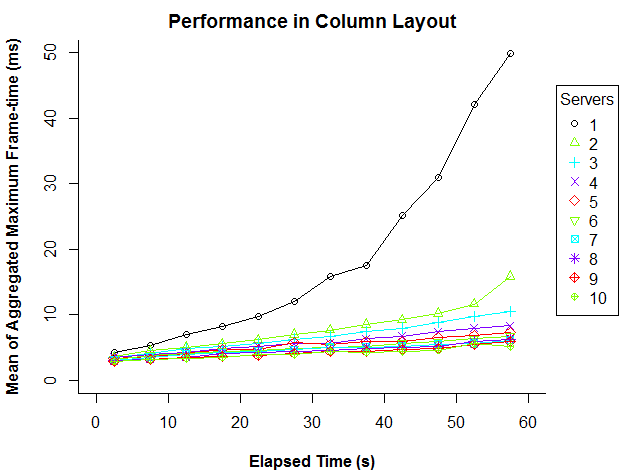
\includegraphics[width=\textwidth]{ColPerformance}
\caption{Performance of increasing numbers of servers with an accumulating number of objects (in column layout)}
\label{fig_PerCol}
\end{figure}

The experiments were run for 60 seconds with an injection rate of 160 objects per second. For all experiments, a speed tolerance of $32m\mathord{\cdot}s^{-1}$ was used, which was the maximum expected speed for any object (based on maximum injection height and velocity, and gravity). The latency tolerance for these experiments was set to $2ms$ (based off measurements of latency between servers) and frame-time tolerance was set to $15ms$ (based off preliminary performance results). A time of $16ms$ was used for the physics time-step. Each experiment was repeated 50 times at various times of day to account for differing performance in cloud resources at different times. For each iteration, the maximum frame time of any server was aggregated for each $5s$ period. The mean of the aggregated maximum frame times of the iterations was then calculated and plotted.

Experiments were conducted using AWS G2.2xlarge servers located within the same geographical region. A G2.2xlarge instance uses a 2.60GHz Intel Xeon E5-2670 CPU with 16GB RAM and an NVIDIA GRID K520 (Kepler) GPU running Ubuntu 18.04 LTS.

Fig. \ref{fig_PerCol} shows the performance of our system with rising server numbers from 1 to 10. The graph clearly shows that the addition of servers lowers the frame time throughout the experiment. This is increasingly noticeable later in the simulation when a greater number of objects are present. For higher server numbers the reduction in maximum frame time is less than for lower numbers, which is as expected as in the ideal case the workload per server would be $1/n$ of the total workload, where $n$ is the number of servers. 

From these observations it can be concluded that this system is scalable in column configuration as the addition of servers results in increased performance.

Experiments were also carried out using servers in a corner layout. The layouts of 3 and 4 servers are shown in Fig. \ref{ServerCorner}, in which the 4 server case is a 2x2 grid with a single corner intersection in the centre. The 9 server case is a 3x3 grid with 4 corner intersections. Injection rates and volume dimensions remain the same as in the column based experiments. Fig. \ref{fig_PerCor} shows the graph illustrating performance. The graph demonstrates that increasing the number of servers lowers the frame time. The additional processing overhead of exchanging more messages with more neighbouring servers in the 9 server experiment is outweighed by the performance gains of additional servers.

From these observations it may be declared that this system is scalable in corner configuration as the addition of servers results in increased performance.

\begin{figure}[!t]
	\begin{subfigure}{.5\textwidth}
		\begin{tikzpicture}[line cap=round,line join=round,>=triangle 45,x=1cm,y=1cm,scale=1.2]
		%	\clip(-3,-1.5) rectangle (3,3);
		\fill[line width=0.8pt,color=rvwvcq,fill=rvwvcq,fill opacity=0.1] (-1,-0.02) -- (1,-0.02) -- (1,-0.22) -- (-1,-0.22) -- cycle;
		\fill[line width=0.8pt,color=rvwvcq,fill=rvwvcq,fill opacity=0.1] (-0.02,2.5) -- (-0.02,0.5) -- (-0.22,0.5) -- (-0.22,2.5) -- cycle;
		\fill[line width=0.8pt,color=rvwvcq,fill=rvwvcq,fill opacity=0.1] (0.22,2.5) -- (0.22,0.5) -- (0.02,0.5) -- (0.02,2.5) -- cycle;
		\fill[line width=0.8pt,color=rvwvcq,fill=rvwvcq,fill opacity=0.1] (-2.5,0.22) -- (-0.5,0.22) -- (-0.5,0.02) -- (-2.5,0.02) -- cycle;
		\fill[line width=0.8pt,color=rvwvcq,fill=rvwvcq,fill opacity=0.1] (0.5,0.22) -- (2.5,0.22) -- (2.5,0.022) -- (0.5,0.022) -- cycle;
		\fill[line width=0.8pt,color=sim,fill=sim,fill opacity=0.1] (-3,3) -- (-3,-2) -- (3,-2) -- (3,3) -- cycle;
		\draw [line width=2pt] (-3,0)-- (3,0);
		\draw [line width=2pt] (0,3)-- (0,0);
		\draw [line width=0.8pt,color=rvwvcq] (-1,-0.02)-- (1,-0.02);
		\draw [line width=0.8pt,color=rvwvcq] (1,-0.02)-- (1,-0.22);
		\draw [line width=0.8pt,color=rvwvcq] (1,-0.22)-- (-1,-0.22);
		\draw [line width=0.8pt,color=rvwvcq] (-1,-0.22)-- (-1,-0.02);
		\draw [line width=0.8pt,color=rvwvcq] (-0.02,2.5)-- (-0.02,0.5);
		\draw [line width=0.8pt,color=rvwvcq] (-0.02,0.5)-- (-0.22,0.5);
		\draw [line width=0.8pt,color=rvwvcq] (-0.22,0.5)-- (-0.22,2.5);
		\draw [line width=0.8pt,color=rvwvcq] (-0.22,2.5)-- (-0.02,2.5);
		\draw [line width=0.8pt,color=rvwvcq] (0.22,2.5)-- (0.22,0.5);
		\draw [line width=0.8pt,color=rvwvcq] (0.22,0.5)-- (0.02,0.5);
		\draw [line width=0.8pt,color=rvwvcq] (0.02,0.5)-- (0.02,2.5);
		\draw [line width=0.8pt,color=rvwvcq] (0.02,2.5)-- (0.22,2.5);
		\draw (-1.5,2.5) node[anchor=center] {Server 0};
		\draw (1.5,2.5) node[anchor=center] {Server 1};
		\draw (0,-1) node[anchor=center] {Server 2};
		\draw [line width=0.8pt,color=rvwvcq] (-2.5,0.22)-- (-0.5,0.22);
		\draw [line width=0.8pt,color=rvwvcq] (-0.5,0.22)-- (-0.5,0.02);
		\draw [line width=0.8pt,color=rvwvcq] (-0.5,0.02)-- (-2.5,0.02);
		\draw [line width=0.8pt,color=rvwvcq] (-2.5,0.02)-- (-2.5,0.22);
		\draw [line width=0.8pt,color=rvwvcq] (0.5,0.22)-- (2.5,0.22);
		\draw [line width=0.8pt,color=rvwvcq] (2.5,0.22)-- (2.5,0.022);
		\draw [line width=0.8pt,color=rvwvcq] (2.5,0.022)-- (0.5,0.022);
		\draw [line width=0.8pt,color=rvwvcq] (0.5,0.022)-- (0.5,0.22);
		\draw [line width=0.8pt,color=rvwvcq] (-1.4,1.6)-- (-1.4,1.4);
		\draw [line width=0.8pt,color=rvwvcq] (-1.4,1.4)-- (-1.6,1.4);
		\draw [line width=0.8pt,color=rvwvcq] (-1.6,1.4)-- (-1.6,1.6);
		\draw [line width=0.8pt,color=rvwvcq] (-1.6,1.6)-- (-1.4,1.6);
		\draw [line width=0.8pt,color=rvwvcq] (1.6,1.6)-- (1.6,1.4);
		\draw [line width=0.8pt,color=rvwvcq] (1.6,1.4)-- (1.4,1.4);
		\draw [line width=0.8pt,color=rvwvcq] (1.4,1.4)-- (1.4,1.6);
		\draw [line width=0.8pt,color=rvwvcq] (1.4,1.6)-- (1.6,1.6);
		
		\draw [line width=0.8pt,color=rvwvcq] (0.1,-1.6)-- (0.1,-1.4);
		\draw [line width=0.8pt,color=rvwvcq] (0.1,-1.4)-- (-0.1,-1.4);
		\draw [line width=0.8pt,color=rvwvcq] (-0.1,-1.4)-- (-0.1,-1.6);
		\draw [line width=0.8pt,color=rvwvcq] (-0.1,-1.6)-- (0.1,-1.6);
		\end{tikzpicture}
		\centering
		\begin{tikzpicture}[line cap=round,line join=round,>=triangle 45,x=1cm,y=1cm]
		%		\clip(-3.661612836111066,-0.55) rectangle (6.690195527240868,1.05);
		\fill[line width=0.8pt,color=rvwvcq,fill=rvwvcq,fill opacity=0.1] (-2.5,0.22) -- (-2.3,0.22) -- (-2.3,0.02) -- (-2.5,0.02) -- cycle;
		\draw [line width=0.8pt,color=rvwvcq] (-2.5,0.22)-- (-2.3,0.22);
		\draw [line width=0.8pt,color=rvwvcq] (-2.3,0.22)-- (-2.3,0.02);
		\draw [line width=0.8pt,color=rvwvcq] (-2.3,0.02)-- (-2.5,0.02);
		\draw [line width=0.8pt,color=rvwvcq] (-2.5,0.02)-- (-2.5,0.22);
		\draw [line width=2pt] (-2.5,0.5)-- (-2.3,0.5);
		\draw (-2.1,0.5) node[anchor=west] {Region Boundary};
		\draw (-2.1,0.1) node[anchor=west] {Injection Volume};
		\end{tikzpicture}
		\caption{3 Server Corner Layout}
		\label{3ServerCorner}
	\end{subfigure}%
	\begin{subfigure}{.5\textwidth}
		\begin{tikzpicture}[line cap=round,line join=round,>=triangle 45,x=1cm,y=1cm,scale=1.2]
		%	\clip(-3,-3) rectangle (3,3);
		\fill[line width=0.8pt,color=rvwvcq,fill=rvwvcq,fill opacity=0.1] (0.5,-0.02) -- (2.5,-0.02) -- (2.5,-0.22) -- (0.5,-0.22) -- cycle;
		\fill[line width=0.8pt,color=rvwvcq,fill=rvwvcq,fill opacity=0.1] (-0.02,2.5) -- (-0.02,0.5) -- (-0.22,0.5) -- (-0.22,2.5) -- cycle;
		\fill[line width=0.8pt,color=rvwvcq,fill=rvwvcq,fill opacity=0.1] (0.22,2.5) -- (0.22,0.5) -- (0.02,0.5) -- (0.02,2.5) -- cycle;
		\fill[line width=0.8pt,color=rvwvcq,fill=rvwvcq,fill opacity=0.1] (-2.5,0.22) -- (-0.5,0.22) -- (-0.5,0.02) -- (-2.5,0.02) -- cycle;
		\fill[line width=0.8pt,color=rvwvcq,fill=rvwvcq,fill opacity=0.1] (0.5,0.22) -- (2.5,0.22) -- (2.5,0.022) -- (0.5,0.022) -- cycle;
		\fill[line width=0.8pt,color=rvwvcq,fill=rvwvcq,fill opacity=0.1] (-0.02,-0.5) -- (-0.02,-2.5) -- (-0.22,-2.5) -- (-0.22,-0.5) -- cycle;
		\fill[line width=0.8pt,color=rvwvcq,fill=rvwvcq,fill opacity=0.1] (0.22,-0.5) -- (0.22,-2.5) -- (0.02,-2.5) -- (0.02,-0.5) -- cycle;
		\fill[line width=0.8pt,color=rvwvcq,fill=rvwvcq,fill opacity=0.1] (-2.5,-0.022) -- (-0.5,-0.022) -- (-0.5,-0.22) -- (-2.5,-0.22) -- cycle;
		\fill[line width=0.8pt,color=sim,fill=sim,fill opacity=0.1] (-3,3) -- (-3,-3) -- (3,-3) -- (3,3) -- cycle;
		\draw [line width=2pt] (-3,0)-- (3,0);
		\draw [line width=2pt] (0,3)-- (0,0);
		\draw [line width=0.8pt,color=rvwvcq] (0.5,-0.02)-- (2.5,-0.02);
		\draw [line width=0.8pt,color=rvwvcq] (2.5,-0.02)-- (2.5,-0.22);
		\draw [line width=0.8pt,color=rvwvcq] (2.5,-0.22)-- (0.5,-0.22);
		\draw [line width=0.8pt,color=rvwvcq] (0.5,-0.22)-- (0.5,-0.02);
		\draw [line width=0.8pt,color=rvwvcq] (-0.02,2.5)-- (-0.02,0.5);
		\draw [line width=0.8pt,color=rvwvcq] (-0.02,0.5)-- (-0.22,0.5);
		\draw [line width=0.8pt,color=rvwvcq] (-0.22,0.5)-- (-0.22,2.5);
		\draw [line width=0.8pt,color=rvwvcq] (-0.22,2.5)-- (-0.02,2.5);
		\draw [line width=0.8pt,color=rvwvcq] (0.22,2.5)-- (0.22,0.5);
		\draw [line width=0.8pt,color=rvwvcq] (0.22,0.5)-- (0.02,0.5);
		\draw [line width=0.8pt,color=rvwvcq] (0.02,0.5)-- (0.02,2.5);
		\draw [line width=0.8pt,color=rvwvcq] (0.02,2.5)-- (0.22,2.5);
		\draw (-1.5,2.5) node[anchor=center] {Server 0};
		\draw (1.5,2.5) node[anchor=center] {Server 1};
		\draw (-1.5,-2.5) node[anchor=center] {Server 2};
		\draw (1.5,-2.5) node[anchor=center] {Server 3};
		\draw [line width=0.8pt,color=rvwvcq] (-2.5,0.22)-- (-0.5,0.22);
		\draw [line width=0.8pt,color=rvwvcq] (-0.5,0.22)-- (-0.5,0.02);
		\draw [line width=0.8pt,color=rvwvcq] (-0.5,0.02)-- (-2.5,0.02);
		\draw [line width=0.8pt,color=rvwvcq] (-2.5,0.02)-- (-2.5,0.22);
		\draw [line width=0.8pt,color=rvwvcq] (0.5,0.22)-- (2.5,0.22);
		\draw [line width=0.8pt,color=rvwvcq] (2.5,0.22)-- (2.5,0.022);
		\draw [line width=0.8pt,color=rvwvcq] (2.5,0.022)-- (0.5,0.022);
		\draw [line width=0.8pt,color=rvwvcq] (0.5,0.022)-- (0.5,0.22);
		\draw [line width=0.8pt,color=rvwvcq] (-0.02,-0.5)-- (-0.02,-2.5);
		\draw [line width=0.8pt,color=rvwvcq] (-0.02,-2.5)-- (-0.22,-2.5);
		\draw [line width=0.8pt,color=rvwvcq] (-0.22,-2.5)-- (-0.22,-0.5);
		\draw [line width=0.8pt,color=rvwvcq] (-0.22,-0.5)-- (-0.02,-0.5);
		\draw [line width=0.8pt,color=rvwvcq] (0.22,-0.5)-- (0.22,-2.5);
		\draw [line width=0.8pt,color=rvwvcq] (0.22,-2.5)-- (0.02,-2.5);
		\draw [line width=0.8pt,color=rvwvcq] (0.02,-2.5)-- (0.02,-0.5);
		\draw [line width=0.8pt,color=rvwvcq] (0.02,-0.5)-- (0.22,-0.5);
		\draw [line width=2pt] (0,0)-- (0,-3);
		\draw [line width=0.8pt,color=rvwvcq] (-2.5,-0.022)-- (-0.5,-0.022);
		\draw [line width=0.8pt,color=rvwvcq] (-0.5,-0.022)-- (-0.5,-0.22);
		\draw [line width=0.8pt,color=rvwvcq] (-0.5,-0.22)-- (-2.5,-0.22);
		\draw [line width=0.8pt,color=rvwvcq] (-2.5,-0.22)-- (-2.5,-0.022);
		\draw [line width=0.8pt,color=rvwvcq] (-1.4,1.6)-- (-1.4,1.4);
		\draw [line width=0.8pt,color=rvwvcq] (-1.4,1.4)-- (-1.6,1.4);
		\draw [line width=0.8pt,color=rvwvcq] (-1.6,1.4)-- (-1.6,1.6);
		\draw [line width=0.8pt,color=rvwvcq] (-1.6,1.6)-- (-1.4,1.6);
		\draw [line width=0.8pt,color=rvwvcq] (1.6,1.6)-- (1.6,1.4);
		\draw [line width=0.8pt,color=rvwvcq] (1.6,1.4)-- (1.4,1.4);
		\draw [line width=0.8pt,color=rvwvcq] (1.4,1.4)-- (1.4,1.6);
		\draw [line width=0.8pt,color=rvwvcq] (1.4,1.6)-- (1.6,1.6);
		
		\draw [line width=0.8pt,color=rvwvcq] (-1.4,-1.6)-- (-1.4,-1.4);
		\draw [line width=0.8pt,color=rvwvcq] (-1.4,-1.4)-- (-1.6,-1.4);
		\draw [line width=0.8pt,color=rvwvcq] (-1.6,-1.4)-- (-1.6,-1.6);
		\draw [line width=0.8pt,color=rvwvcq] (-1.6,-1.6)-- (-1.4,-1.6);
		\draw [line width=0.8pt,color=rvwvcq] (1.6,-1.6)-- (1.6,-1.4);
		\draw [line width=0.8pt,color=rvwvcq] (1.6,-1.4)-- (1.4,-1.4);
		\draw [line width=0.8pt,color=rvwvcq] (1.4,-1.4)-- (1.4,-1.6);
		\draw [line width=0.8pt,color=rvwvcq] (1.4,-1.6)-- (1.6,-1.6);
		\end{tikzpicture}
		\centering
		\caption{4 Server Corner Layout}
		\label{4ServerCorner}
	\end{subfigure}
\caption{Corner Layouts}
\label{ServerCorner}
\end{figure}

\begin{figure}[!t]
	\begin{tikzpicture}[line cap=round,line join=round,>=triangle 45,x=1cm,y=1cm]
	\fill[line width=0.8pt,color=sim,fill=sim,fill opacity=0.1] (-3,3) -- (-3,-6) -- (6,-6) -- (6,3) -- cycle;
	\draw [line width=2pt] (-3,0)-- (6,0);
	\draw [line width=2pt] (0,3)-- (0,-6);
	\draw [line width=2pt] (-3,-3)-- (6,-3);
	\draw [line width=2pt] (3,3)-- (3,-6);
	\draw (-1.5,2.5) node[anchor=center] {Server 0};
	\draw (1.5,2.5) node[anchor=center] {Server 1};
	\draw (4.5,2.5) node[anchor=center] {Server 2};
	\draw (-1.5,-0.5) node[anchor=center] {Server 3};
	\draw (1.5,-0.5) node[anchor=center] {Server 4};
	\draw (4.5,-0.5) node[anchor=center] {Server 5};
	\draw (-1.5,-3.5) node[anchor=center] {Server 6};
	\draw (1.5,-3.5) node[anchor=center] {Server 7};
	\draw (4.5,-3.5) node[anchor=center] {Server 8};
	
	%Injection volume
	% 4 -> 1
	\fill[line width=0.8pt,color=rvwvcq,fill=rvwvcq,fill opacity=0.1] (0.5,-0.02) -- (2.5,-0.02) -- (2.5,-0.22) -- (0.5,-0.22) -- cycle;
	% 0 -> 1
	\fill[line width=0.8pt,color=rvwvcq,fill=rvwvcq,fill opacity=0.1] (-0.02,2.5) -- (-0.02,0.5) -- (-0.22,0.5) -- (-0.22,2.5) -- cycle;
	% 1 -> 0
	\fill[line width=0.8pt,color=rvwvcq,fill=rvwvcq,fill opacity=0.1] (0.22,2.5) -- (0.22,0.5) -- (0.02,0.5) -- (0.02,2.5) -- cycle;
	% 0 -> 3
	\fill[line width=0.8pt,color=rvwvcq,fill=rvwvcq,fill opacity=0.1] (-2.5,0.22) -- (-0.5,0.22) -- (-0.5,0.02) -- (-2.5,0.02) -- cycle;
	% 1 -> 4
	\fill[line width=0.8pt,color=rvwvcq,fill=rvwvcq,fill opacity=0.1] (0.5,0.22) -- (2.5,0.22) -- (2.5,0.022) -- (0.5,0.022) -- cycle;
	% 3 -> 4
	\fill[line width=0.8pt,color=rvwvcq,fill=rvwvcq,fill opacity=0.1] (-0.02,-0.5) -- (-0.02,-2.5) -- (-0.22,-2.5) -- (-0.22,-0.5) -- cycle;
	% 4 -> 3
	\fill[line width=0.8pt,color=rvwvcq,fill=rvwvcq,fill opacity=0.1] (0.22,-0.5) -- (0.22,-2.5) -- (0.02,-2.5) -- (0.02,-0.5) -- cycle;
	% 3 -> 0
	\fill[line width=0.8pt,color=rvwvcq,fill=rvwvcq,fill opacity=0.1] (-2.5,-0.022) -- (-0.5,-0.022) -- (-0.5,-0.22) -- (-2.5,-0.22) -- cycle;
	
	% 5 -> 2
	\fill[line width=0.8pt,color=rvwvcq,fill=rvwvcq,fill opacity=0.1] (3.5,-0.02) -- (5.5,-0.02) -- (5.5,-0.22) -- (3.5,-0.22) -- cycle;
	% 6 -> 3
	\fill[line width=0.8pt,color=rvwvcq,fill=rvwvcq,fill opacity=0.1] (-2.5,-3.022) -- (-0.5,-3.022) -- (-0.5,-3.22) -- (-2.5,-3.22) -- cycle;
	% 7 -> 4
	\fill[line width=0.8pt,color=rvwvcq,fill=rvwvcq,fill opacity=0.1] (0.5,-3.022) -- (2.5,-3.022) -- (2.5,-3.22) -- (0.5,-3.22) -- cycle;
	% 8 -> 5
	\fill[line width=0.8pt,color=rvwvcq,fill=rvwvcq,fill opacity=0.1] (3.5,-3.022) -- (5.5,-3.022) -- (5.5,-3.22) -- (3.5,-3.22) -- cycle;
	% 2 -> 5
	\fill[line width=0.8pt,color=rvwvcq,fill=rvwvcq,fill opacity=0.1] (3.5,0.22) -- (5.5,0.22) -- (5.5,0.022) -- (3.5,0.022) -- cycle;
	% 3 -> 6
	\fill[line width=0.8pt,color=rvwvcq,fill=rvwvcq,fill opacity=0.1] (-2.5,-2.78) -- (-0.5,-2.78) -- (-0.5,-2.978) -- (-2.5,-2.978) -- cycle;
	% 4 -> 7
	\fill[line width=0.8pt,color=rvwvcq,fill=rvwvcq,fill opacity=0.1] (0.5,-2.78) -- (2.5,-2.78) -- (2.5,-2.978) -- (0.5,-2.978) -- cycle;
	% 5 -> 8
	\fill[line width=0.8pt,color=rvwvcq,fill=rvwvcq,fill opacity=0.1] (3.5,-2.78) -- (5.5,-2.78) -- (5.5,-2.978) -- (3.5,-2.978) -- cycle;
	% 1 -> 2
	\fill[line width=0.8pt,color=rvwvcq,fill=rvwvcq,fill opacity=0.1] (2.978,2.5) -- (2.978,0.5) -- (2.78,0.5) -- (2.78,2.5) -- cycle;
	% 4 -> 5
	\fill[line width=0.8pt,color=rvwvcq,fill=rvwvcq,fill opacity=0.1] (2.978,-0.5) -- (2.978,-2.5) -- (2.78,-2.5) -- (2.78,-0.5) -- cycle;
	% 6 -> 7
	\fill[line width=0.8pt,color=rvwvcq,fill=rvwvcq,fill opacity=0.1] (-0.02,-3.5) -- (-0.02,-5.5) -- (-0.22,-5.5) -- (-0.22,-3.5) -- cycle;
	% 7 -> 8
	\fill[line width=0.8pt,color=rvwvcq,fill=rvwvcq,fill opacity=0.1] (2.978,-3.5) -- (2.978,-5.5) -- (2.78,-5.5) -- (2.78,-3.5) -- cycle;
	% 7 -> 6
	\fill[line width=0.8pt,color=rvwvcq,fill=rvwvcq,fill opacity=0.1] (0.22,-3.5) -- (0.22,-5.5) -- (0.02,-5.5) -- (0.02,-3.5) -- cycle;
	% 2 -> 1
	\fill[line width=0.8pt,color=rvwvcq,fill=rvwvcq,fill opacity=0.1] (3.22,2.5) -- (3.22,0.5) -- (3.02,0.5) -- (3.02,2.5) -- cycle;
	% 5 -> 4
	\fill[line width=0.8pt,color=rvwvcq,fill=rvwvcq,fill opacity=0.1] (3.22,-0.5) -- (3.22,-2.5) -- (3.02,-2.5) -- (3.02,-0.5) -- cycle;
	% 8 -> 7
	\fill[line width=0.8pt,color=rvwvcq,fill=rvwvcq,fill opacity=0.1] (3.22,-3.5) -- (3.22,-5.5) -- (3.02,-5.5) -- (3.02,-3.5) -- cycle;
	
	
	% 4 -> 1
	\draw [line width=0.8pt,color=rvwvcq] (0.5,-0.02)-- (2.5,-0.02);
	\draw [line width=0.8pt,color=rvwvcq] (2.5,-0.02)-- (2.5,-0.22);
	\draw [line width=0.8pt,color=rvwvcq] (2.5,-0.22)-- (0.5,-0.22);
	\draw [line width=0.8pt,color=rvwvcq] (0.5,-0.22)-- (0.5,-0.02);
	
	% 5 -> 2
	\draw [line width=0.8pt,color=rvwvcq] (3.5,-0.02)-- (5.5,-0.02);
	\draw [line width=0.8pt,color=rvwvcq] (5.5,-0.02)-- (5.5,-0.22);
	\draw [line width=0.8pt,color=rvwvcq] (5.5,-0.22)-- (3.5,-0.22);
	\draw [line width=0.8pt,color=rvwvcq] (3.5,-0.22)-- (3.5,-0.02);
	
	% 0 -> 1
	\draw [line width=0.8pt,color=rvwvcq] (-0.02,2.5)-- (-0.02,0.5);
	\draw [line width=0.8pt,color=rvwvcq] (-0.02,0.5)-- (-0.22,0.5);
	\draw [line width=0.8pt,color=rvwvcq] (-0.22,0.5)-- (-0.22,2.5);
	\draw [line width=0.8pt,color=rvwvcq] (-0.22,2.5)-- (-0.02,2.5);
	
	% 1 -> 2
	\draw [line width=0.8pt,color=rvwvcq] (2.98,2.5)-- (2.98,0.5);
	\draw [line width=0.8pt,color=rvwvcq] (2.98,0.5)-- (2.78,0.5);
	\draw [line width=0.8pt,color=rvwvcq] (2.78,0.5)-- (2.78,2.5);
	\draw [line width=0.8pt,color=rvwvcq] (2.78,2.5)-- (2.98,2.5);
	
	% 1 -> 0
	\draw [line width=0.8pt,color=rvwvcq] (0.22,2.5)-- (0.22,0.5);
	\draw [line width=0.8pt,color=rvwvcq] (0.22,0.5)-- (0.02,0.5);
	\draw [line width=0.8pt,color=rvwvcq] (0.02,0.5)-- (0.02,2.5);
	\draw [line width=0.8pt,color=rvwvcq] (0.02,2.5)-- (0.22,2.5);
	
	% 2 -> 1
	\draw [line width=0.8pt,color=rvwvcq] (3.22,2.5)-- (3.22,0.5);
	\draw [line width=0.8pt,color=rvwvcq] (3.22,0.5)-- (3.02,0.5);
	\draw [line width=0.8pt,color=rvwvcq] (3.02,0.5)-- (3.02,2.5);
	\draw [line width=0.8pt,color=rvwvcq] (3.02,2.5)-- (3.22,2.5);
	
	% 0 -> 3
	\draw [line width=0.8pt,color=rvwvcq] (-2.5,0.22)-- (-0.5,0.22);
	\draw [line width=0.8pt,color=rvwvcq] (-0.5,0.22)-- (-0.5,0.02);
	\draw [line width=0.8pt,color=rvwvcq] (-0.5,0.02)-- (-2.5,0.02);
	\draw [line width=0.8pt,color=rvwvcq] (-2.5,0.02)-- (-2.5,0.22);
	
	% 1 -> 4
	\draw [line width=0.8pt,color=rvwvcq] (0.5,0.22)-- (2.5,0.22);
	\draw [line width=0.8pt,color=rvwvcq] (2.5,0.22)-- (2.5,0.022);
	\draw [line width=0.8pt,color=rvwvcq] (2.5,0.022)-- (0.5,0.022);
	\draw [line width=0.8pt,color=rvwvcq] (0.5,0.022)-- (0.5,0.22);
	
	% 2 -> 5
	\draw [line width=0.8pt,color=rvwvcq] (3.5,0.22)-- (5.5,0.22);
	\draw [line width=0.8pt,color=rvwvcq] (5.5,0.22)-- (5.5,0.022);
	\draw [line width=0.8pt,color=rvwvcq] (5.5,0.022)-- (3.5,0.022);
	\draw [line width=0.8pt,color=rvwvcq] (3.5,0.022)-- (3.5,0.22);
	
	% 3 -> 6
	\draw [line width=0.8pt,color=rvwvcq] (-2.5,-3.22)-- (-0.5,-3.22);
	\draw [line width=0.8pt,color=rvwvcq] (-0.5,-3.22)-- (-0.5,-3.02);
	\draw [line width=0.8pt,color=rvwvcq] (-0.5,-3.02)-- (-2.5,-3.02);
	\draw [line width=0.8pt,color=rvwvcq] (-2.5,-3.02)-- (-2.5,-3.22);
	
	% 4 -> 7
	\draw [line width=0.8pt,color=rvwvcq] (0.5,-3.22)-- (2.5,-3.22);
	\draw [line width=0.8pt,color=rvwvcq] (2.5,-3.22)-- (2.5,-3.022);
	\draw [line width=0.8pt,color=rvwvcq] (2.5,-3.022)-- (0.5,-3.022);
	\draw [line width=0.8pt,color=rvwvcq] (0.5,-3.022)-- (0.5,-3.22);
	
	% 5 -> 8
	\draw [line width=0.8pt,color=rvwvcq] (3.5,-3.22)-- (5.5,-3.22);
	\draw [line width=0.8pt,color=rvwvcq] (5.5,-3.22)-- (5.5,-3.022);
	\draw [line width=0.8pt,color=rvwvcq] (5.5,-3.022)-- (3.5,-3.022);
	\draw [line width=0.8pt,color=rvwvcq] (3.5,-3.022)-- (3.5,-3.22);
	
	% 3 -> 4
	\draw [line width=0.8pt,color=rvwvcq] (-0.02,-0.5)-- (-0.02,-2.5);
	\draw [line width=0.8pt,color=rvwvcq] (-0.02,-2.5)-- (-0.22,-2.5);
	\draw [line width=0.8pt,color=rvwvcq] (-0.22,-2.5)-- (-0.22,-0.5);
	\draw [line width=0.8pt,color=rvwvcq] (-0.22,-0.5)-- (-0.02,-0.5);
	
	% 4 -> 5
	\draw [line width=0.8pt,color=rvwvcq] (2.98,-0.5)-- (2.98,-2.5);
	\draw [line width=0.8pt,color=rvwvcq] (2.98,-2.5)-- (2.78,-2.5);
	\draw [line width=0.8pt,color=rvwvcq] (2.78,-2.5)-- (2.78,-0.5);
	\draw [line width=0.8pt,color=rvwvcq] (2.78,-0.5)-- (2.98,-0.5);
	
	% 6 -> 7
	\draw [line width=0.8pt,color=rvwvcq] (-0.02,-3.5)-- (-0.02,-5.5);
	\draw [line width=0.8pt,color=rvwvcq] (-0.02,-5.5)-- (-0.22,-5.5);
	\draw [line width=0.8pt,color=rvwvcq] (-0.22,-5.5)-- (-0.22,-3.5);
	\draw [line width=0.8pt,color=rvwvcq] (-0.22,-3.5)-- (-0.02,-3.5);
	
	% 7 -> 8
	\draw [line width=0.8pt,color=rvwvcq] (2.98,-3.5)-- (2.98,-5.5);
	\draw [line width=0.8pt,color=rvwvcq] (2.98,-5.5)-- (2.78,-5.5);
	\draw [line width=0.8pt,color=rvwvcq] (2.78,-5.5)-- (2.78,-3.5);
	\draw [line width=0.8pt,color=rvwvcq] (2.78,-3.5)-- (2.98,-3.5);
	
	% 4 -> 3
	\draw [line width=0.8pt,color=rvwvcq] (0.22,-0.5)-- (0.22,-2.5);
	\draw [line width=0.8pt,color=rvwvcq] (0.22,-2.5)-- (0.02,-2.5);
	\draw [line width=0.8pt,color=rvwvcq] (0.02,-2.5)-- (0.02,-0.5);
	\draw [line width=0.8pt,color=rvwvcq] (0.02,-0.5)-- (0.22,-0.5);
	
	% 5 -> 4
	\draw [line width=0.8pt,color=rvwvcq] (3.22,-0.5)-- (3.22,-2.5);
	\draw [line width=0.8pt,color=rvwvcq] (3.22,-2.5)-- (3.02,-2.5);
	\draw [line width=0.8pt,color=rvwvcq] (3.02,-2.5)-- (3.02,-0.5);
	\draw [line width=0.8pt,color=rvwvcq] (3.02,-0.5)-- (3.22,-0.5);
	
	% 3 -> 0
	\draw [line width=0.8pt,color=rvwvcq] (-2.5,-0.022)-- (-0.5,-0.022);
	\draw [line width=0.8pt,color=rvwvcq] (-0.5,-0.022)-- (-0.5,-0.22);
	\draw [line width=0.8pt,color=rvwvcq] (-0.5,-0.22)-- (-2.5,-0.22);
	\draw [line width=0.8pt,color=rvwvcq] (-2.5,-0.22)-- (-2.5,-0.022);
	
	% 7 -> 6
	\draw [line width=0.8pt,color=rvwvcq] (0.22,-3.5)-- (0.22,-5.5);
	\draw [line width=0.8pt,color=rvwvcq] (0.22,-5.5)-- (0.02,-5.5);
	\draw [line width=0.8pt,color=rvwvcq] (0.02,-5.5)-- (0.02,-3.5);
	\draw [line width=0.8pt,color=rvwvcq] (0.02,-3.5)-- (0.22,-3.5);
	
	% 8 -> 7
	\draw [line width=0.8pt,color=rvwvcq] (3.22,-3.5)-- (3.22,-5.5);
	\draw [line width=0.8pt,color=rvwvcq] (3.22,-5.5)-- (3.02,-5.5);
	\draw [line width=0.8pt,color=rvwvcq] (3.02,-5.5)-- (3.02,-3.5);
	\draw [line width=0.8pt,color=rvwvcq] (3.02,-3.5)-- (3.22,-3.5);
	
	% 3 -> 6
	\draw [line width=0.8pt,color=rvwvcq] (-2.5,-2.78)-- (-0.5,-2.78);
	\draw [line width=0.8pt,color=rvwvcq] (-0.5,-2.78)-- (-0.5,-2.978);
	\draw [line width=0.8pt,color=rvwvcq] (-0.5,-2.978)-- (-2.5,-2.978);
	\draw [line width=0.8pt,color=rvwvcq] (-2.5,-2.978)-- (-2.5,-2.78);
	
	% 4 -> 7
	\draw [line width=0.8pt,color=rvwvcq] (0.5,-2.78)-- (2.5,-2.78);
	\draw [line width=0.8pt,color=rvwvcq] (2.5,-2.78)-- (2.5,-2.978);
	\draw [line width=0.8pt,color=rvwvcq] (2.5,-2.978)-- (0.5,-2.978);
	\draw [line width=0.8pt,color=rvwvcq] (0.5,-2.978)-- (0.5,-2.78);
	
	% 5 -> 8
	\draw [line width=0.8pt,color=rvwvcq] (3.5,-2.78)-- (5.5,-2.78);
	\draw [line width=0.8pt,color=rvwvcq] (5.5,-2.78)-- (5.5,-2.978);
	\draw [line width=0.8pt,color=rvwvcq] (5.5,-2.978)-- (3.5,-2.978);
	\draw [line width=0.8pt,color=rvwvcq] (3.5,-2.978)-- (3.5,-2.78);
	
	% Server 0
	\draw [line width=0.8pt,color=rvwvcq] (-1.4,1.6)-- (-1.4,1.4);
	\draw [line width=0.8pt,color=rvwvcq] (-1.4,1.4)-- (-1.6,1.4);
	\draw [line width=0.8pt,color=rvwvcq] (-1.6,1.4)-- (-1.6,1.6);
	\draw [line width=0.8pt,color=rvwvcq] (-1.6,1.6)-- (-1.4,1.6);
	
	% Server 1
	\draw [line width=0.8pt,color=rvwvcq] (1.6,1.6)-- (1.6,1.4);
	\draw [line width=0.8pt,color=rvwvcq] (1.6,1.4)-- (1.4,1.4);
	\draw [line width=0.8pt,color=rvwvcq] (1.4,1.4)-- (1.4,1.6);
	\draw [line width=0.8pt,color=rvwvcq] (1.4,1.6)-- (1.6,1.6);
	
	% Server 2
	\draw [line width=0.8pt,color=rvwvcq] (4.6,1.6)-- (4.6,1.4);
	\draw [line width=0.8pt,color=rvwvcq] (4.6,1.4)-- (4.4,1.4);
	\draw [line width=0.8pt,color=rvwvcq] (4.4,1.4)-- (4.4,1.6);
	\draw [line width=0.8pt,color=rvwvcq] (4.4,1.6)-- (4.6,1.6);
	
	% Server 3
	\draw [line width=0.8pt,color=rvwvcq] (-1.4,-1.6)-- (-1.4,-1.4);
	\draw [line width=0.8pt,color=rvwvcq] (-1.4,-1.4)-- (-1.6,-1.4);
	\draw [line width=0.8pt,color=rvwvcq] (-1.6,-1.4)-- (-1.6,-1.6);
	\draw [line width=0.8pt,color=rvwvcq] (-1.6,-1.6)-- (-1.4,-1.6);
	
	% Server 4
	\draw [line width=0.8pt,color=rvwvcq] (1.6,-1.6)-- (1.6,-1.4);
	\draw [line width=0.8pt,color=rvwvcq] (1.6,-1.4)-- (1.4,-1.4);
	\draw [line width=0.8pt,color=rvwvcq] (1.4,-1.4)-- (1.4,-1.6);
	\draw [line width=0.8pt,color=rvwvcq] (1.4,-1.6)-- (1.6,-1.6);
	
	% Server 5
	\draw [line width=0.8pt,color=rvwvcq] (4.6,-1.6)-- (4.6,-1.4);
	\draw [line width=0.8pt,color=rvwvcq] (4.6,-1.4)-- (4.4,-1.4);
	\draw [line width=0.8pt,color=rvwvcq] (4.4,-1.4)-- (4.4,-1.6);
	\draw [line width=0.8pt,color=rvwvcq] (4.4,-1.6)-- (4.6,-1.6);
	
	% Server 6
	\draw [line width=0.8pt,color=rvwvcq] (-1.4,-4.6)-- (-1.4,-4.4);
	\draw [line width=0.8pt,color=rvwvcq] (-1.4,-4.4)-- (-1.6,-4.4);
	\draw [line width=0.8pt,color=rvwvcq] (-1.6,-4.4)-- (-1.6,-4.6);
	\draw [line width=0.8pt,color=rvwvcq] (-1.6,-4.6)-- (-1.4,-4.6);
	
	% Server 7
	\draw [line width=0.8pt,color=rvwvcq] (1.6,-4.6)-- (1.6,-4.4);
	\draw [line width=0.8pt,color=rvwvcq] (1.6,-4.4)-- (1.4,-4.4);
	\draw [line width=0.8pt,color=rvwvcq] (1.4,-4.4)-- (1.4,-4.6);
	\draw [line width=0.8pt,color=rvwvcq] (1.4,-4.6)-- (1.6,-4.6);
	
	% Server 8
	\draw [line width=0.8pt,color=rvwvcq] (4.6,-4.6)-- (4.6,-4.4);
	\draw [line width=0.8pt,color=rvwvcq] (4.6,-4.4)-- (4.4,-4.4);
	\draw [line width=0.8pt,color=rvwvcq] (4.4,-4.4)-- (4.4,-4.6);
	\draw [line width=0.8pt,color=rvwvcq] (4.4,-4.6)-- (4.6,-4.6);
	
	\end{tikzpicture}
	\centering
	\begin{tikzpicture}[line cap=round,line join=round,>=triangle 45,x=1cm,y=1cm]
	\clip(-4,0) rectangle (7,1.5);
	\draw [line width=2pt] (-3.5,0.7)-- (-3.3,0.7);
	\draw (-3.1,0.7) node[anchor=west] {Server-Region Boundary};
	
	\fill[line width=0.8pt,color=rvwvcq,fill=rvwvcq,fill opacity=0.1] (2.5,0.82) -- (2.3,0.82) -- (2.3,0.62) -- (2.5,0.62) -- cycle;
	\draw [line width=0.8pt,color=rvwvcq] (2.5,0.82)-- (2.3,0.82);
	\draw [line width=0.8pt,color=rvwvcq] (2.3,0.82)-- (2.3,0.62);
	\draw [line width=0.8pt,color=rvwvcq] (2.3,0.62)-- (2.5,0.62);
	\draw [line width=0.8pt,color=rvwvcq] (2.5,0.62)-- (2.5,0.82);
	
	\draw (2.7,0.7) node[anchor=west] {Injection Volume};
	\end{tikzpicture}
	\caption{9 Server Corner Layout}
	\label{3x3Servers}
\end{figure}

\begin{figure}[!t]
	\centering
	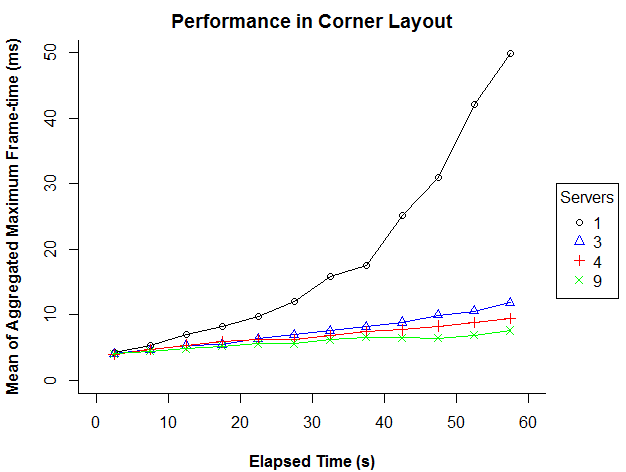
\includegraphics[width=\textwidth]{CorPerformance}
	\caption{Performance of increasing numbers of servers with an accumulating number of objects (in corner layout)}
	\label{fig_PerCor}
\end{figure}
\clearpage
\section{Collision Correctness Experiments}
In the following section the correctness of collisions between objects is explored, i.e. do objects have the same collision behaviour in a AP as they do in a centralised system.

The following points highlight the contributions of the correctness experiments:
\begin{itemize}
	\item Demonstrate that collisions between objects and migrating are handled correctly as long as the factors (speed, frame-time, latency) remain within their tolerances. Collisions can be handled correctly under worsening conditions (higher object speed, frame-time and latency), so long as the tolerances account for these.
	\item Demonstrate that late collisions begin to occur once tolerances are exceeded or as predicted by the aura calculation, i.e. auras are the size they need to be, and no larger, which would impact on performance.
	\item Demonstrate the severity of each of the factors being exceeded, i.e. when different factors are exceeded, how badly are collisions handled?
	\item Measure the frequency of two-object-thrashing
\end{itemize}

Experiments were undertaken to detect erroneous collisions under different conditions and are concerned with objects that are migrating and/or interacting with an object that has recently migrated. Erroneous collisions fall into two categories:
\begin{itemize}
	\item Missed collisions - collisions that should have taken place but were not detected by the physics engine e.g. Bullet through paper problem.
	\item Late collisions - collisions that were detected later than expected in a centralised simulation and result in not only different collision results, but also unstable collision response.
\end{itemize}

%To understand how late collisions lead to unstable collision response, we must first understand how in real-time collision detection works. In real-time physics engines, objects move in discrete steps, as a result of this, when two objects collide, they overlap each other i.e. penetrate. The collision is resolved by calculating the forces resulting from the collision and moving the objects so they no longer overlap (in PhysX if penetration is high, the latter may be done over several physics time-steps). If the penetration is high, such as in the case of a late collision response or if two objects are moving at high speed towards one another, the collision response can no longer guarantee stable results.

%It is possible to detect late collisions between objects. Given the relative speed of the two objects and the physics time-step, it possible to calculate the maximum expected penetration distance. If a collision is detected and it is above this value, it means it is a late collision.

%Maximum penetration for a given speed occurs when two objects travelling directly towards each other have, in the final time-step before colliding the two objects have no distance between them, but are not overlapping, so not colliding. The next physics time-step, the collision will be detected and will have the maximum penetration possible for that relative speed. Re-arranging $s=d/t$, to $d=s.t$ and substituting the physics time-step for $t$, gives us the maximum distance (penetration) for a relative speed, and we are able to plot the maximum expected penetration line.

%In real-time physics, speed of calculation is favoured over accuracy of collision response, as a result of this 

%, this is known as the collision response (in real-time physics, speed of calculation is favoured over accuracy of collision response). High collision penetration e.g. if two objects are moving quickly towards one another, can lead to unstable collision response, which is undesirable.

%Experiments were carried out where collision results were recorded and used to detect missed and late collisions of objects. The experiment scenario used only two objects, meaning if there was a missed collision there would be no collision output. The two objects start the scenario with a specified velocity (drag and gravity are disabled), the direction being directly towards the other object and the two objects were given the same speed, which is varied throughout the experiment. Spheres were used, so rotational effects don't need to be accounted for.

A recap of how a naive system can lead to erroneous collision behaviour and how AP can lead to erroneous collision behaviour if speed, frame-time, or latency exceed the user-defined tolerances will now be given.

In a hypothetical naive system, a system that does not use AP, objects are migrated solely based on their position and objects on a remote server are not accounted for. Two objects close to the server region boundary could be occupying the same space at the same time. If one object were to be migrated to the other server, for example, if the centre of the object has traversed the region boundary, then the object would be migrated into an overlapping space as the other object on the receiving server. This penetration could be much greater than would be expected in a normal collision detection and could lead to a highly erroneous collision response.

AP works by predicting the future bounding sphere of both the object projecting the aura and a potential object on the remote server. When an object collides with an aura from a remote server, the object is migrated to the owner of the aura. However, the aura projection is not instantaneous and has to account for the following three factors: the speeds of both objects; the frame-times of the two servers; and the latency between the two servers. These three factors need to be known through the duration between the aura projection being initiated and a remote object being received and collided with. As it not possible to know these three factors in advance, tolerances must be used. These three tolerances are used to determine the size of the aura with the aim to ensure a remote object is migrated before a collision happens. If the speed tolerance is exceeded, an object can penetrate deeper into the aura than the maximum penetration to ensure it is migrated in time before a collision occurs. In the case of latency, the aura would potentially arrive too late on the receiving server, meaning the migration is triggered too late. In addition to this, the migrating object's arrival will be delayed, potentially leading to a late collision. In the case of frame-time, the extra delay between the messages being processed and physics time-step could cause the collision with the aura to be detected too late and potentially lead to a late collision. Furthermore, the extra delay between the migration message being received and the object being present in the physics simulation on the receiving server could cause the collision to be detected too late.

%TODO: Expand on late collisions producing different results?

%TODO: The following paragraph should probably be in a section about why late collisions are bad and why we want to avoid them.
To understand how late collisions lead to unstable collision response, it must first be understood how in real-time collision detection works, which is discussed in \ref{collision_detection}. In summary, in real-time physics engines, objects move in discrete steps. As a result of this, when two objects collide, they overlap each other i.e. penetrate. The collision is resolved by calculating the forces resulting from the collision and moving the objects so they no longer overlap (in PhysX if penetration is high, the latter may be done over several physics time-steps). If the penetration is high, such as in the case of a late collision response or if two objects are moving at high speed towards one another, the collision response can no longer guarantee stable results.

\subsection{Collision Error Detection}
It is possible to detect late collisions between objects; Given the relative speed of the two objects and the physics time-step, it is possible to calculate the maximum expected penetration distance. If a collision is detected and it is above this value, it means it is a late collision. In addition, if no collisions occur, it means there is a missed collision.

Collision penetration can range from 0 to maximum penetration distance and depends upon the distance between the two objects' surfaces in the time-step before the collision. Maximum penetration for a given speed occurs when two objects are travelling directly towards each other and in the time-step before the collision occurs, there is no distance between the surfaces of the objects. In the next time-step, this results in the two objects overlapping each other with the maximum penetration for their relative speed. The overlap is then detected as a collision by the physics engine. Re-arranging $s=d/t$, to $d=s.t$ and substituting the physics time-step for $t$, gives us the maximum distance (penetration) for a relative speed, and we are able to plot the maximum expected penetration line.

%In real-time physics, speed of calculation is favoured over accuracy of collision response, as a result of this 

%, this is known as the collision response (in real-time physics, speed of calculation is favoured over accuracy of collision response). High collision penetration e.g. if two objects are moving quickly towards one another, can lead to unstable collision response, which is undesirable.

%TODO: cite that deep penetration is bad

In all the following experiments collisions were recorded, for each collision, the following data is contained: Relative Speed, the speed of the two colliding objects relative to each other; Penetration, the distance the two objects overlapped when the collision was detected. PhysX reports penetration of collisions as negative values and can report collisions before the two objects are intersecting, which is recorded as a positive penetration. In all experiments, the penetration is negated for simplicity. The relative speed and penetration can be used to determine if the collision was a late collision. In all the following experimental scenarios only two objects are used, meaning if there was a missed collision there would be no collision output and multiple collisions from the same pair of objects can be ignored. The two objects start the scenario with a specified velocity (drag and gravity are disabled), the direction being directly towards the other object and the two objects were given the same speed and a random variation of between $0$ and $-1m\mathord{\cdot}s^{-1}$ to prevent identical results between iterations. Spheres were used, so rotational effects, such as rotational velocity, do not need to be accounted for. 

Thrashing between two objects on different servers is an unsolved problem in AP; thrashing occurrences can be detected by counting the number of migrations that occur before the first collision is detected, as only two objects are involved in each experiment, the number of migrations before a collision should only be one, otherwise thrashing has occurred. For the purposes of these experiments, collisions involving thrashing will be excluded, regardless of the correctness of the collision. For the remainder of this chapter, thrashing refers to only thrashing between two objects and not the solved 3-object-thrashing problem.

%TODO: Some justifcation for exluding thrashing?

\subsection{Control Experiment}

%\begin{figure}[t]
%	\centering
%	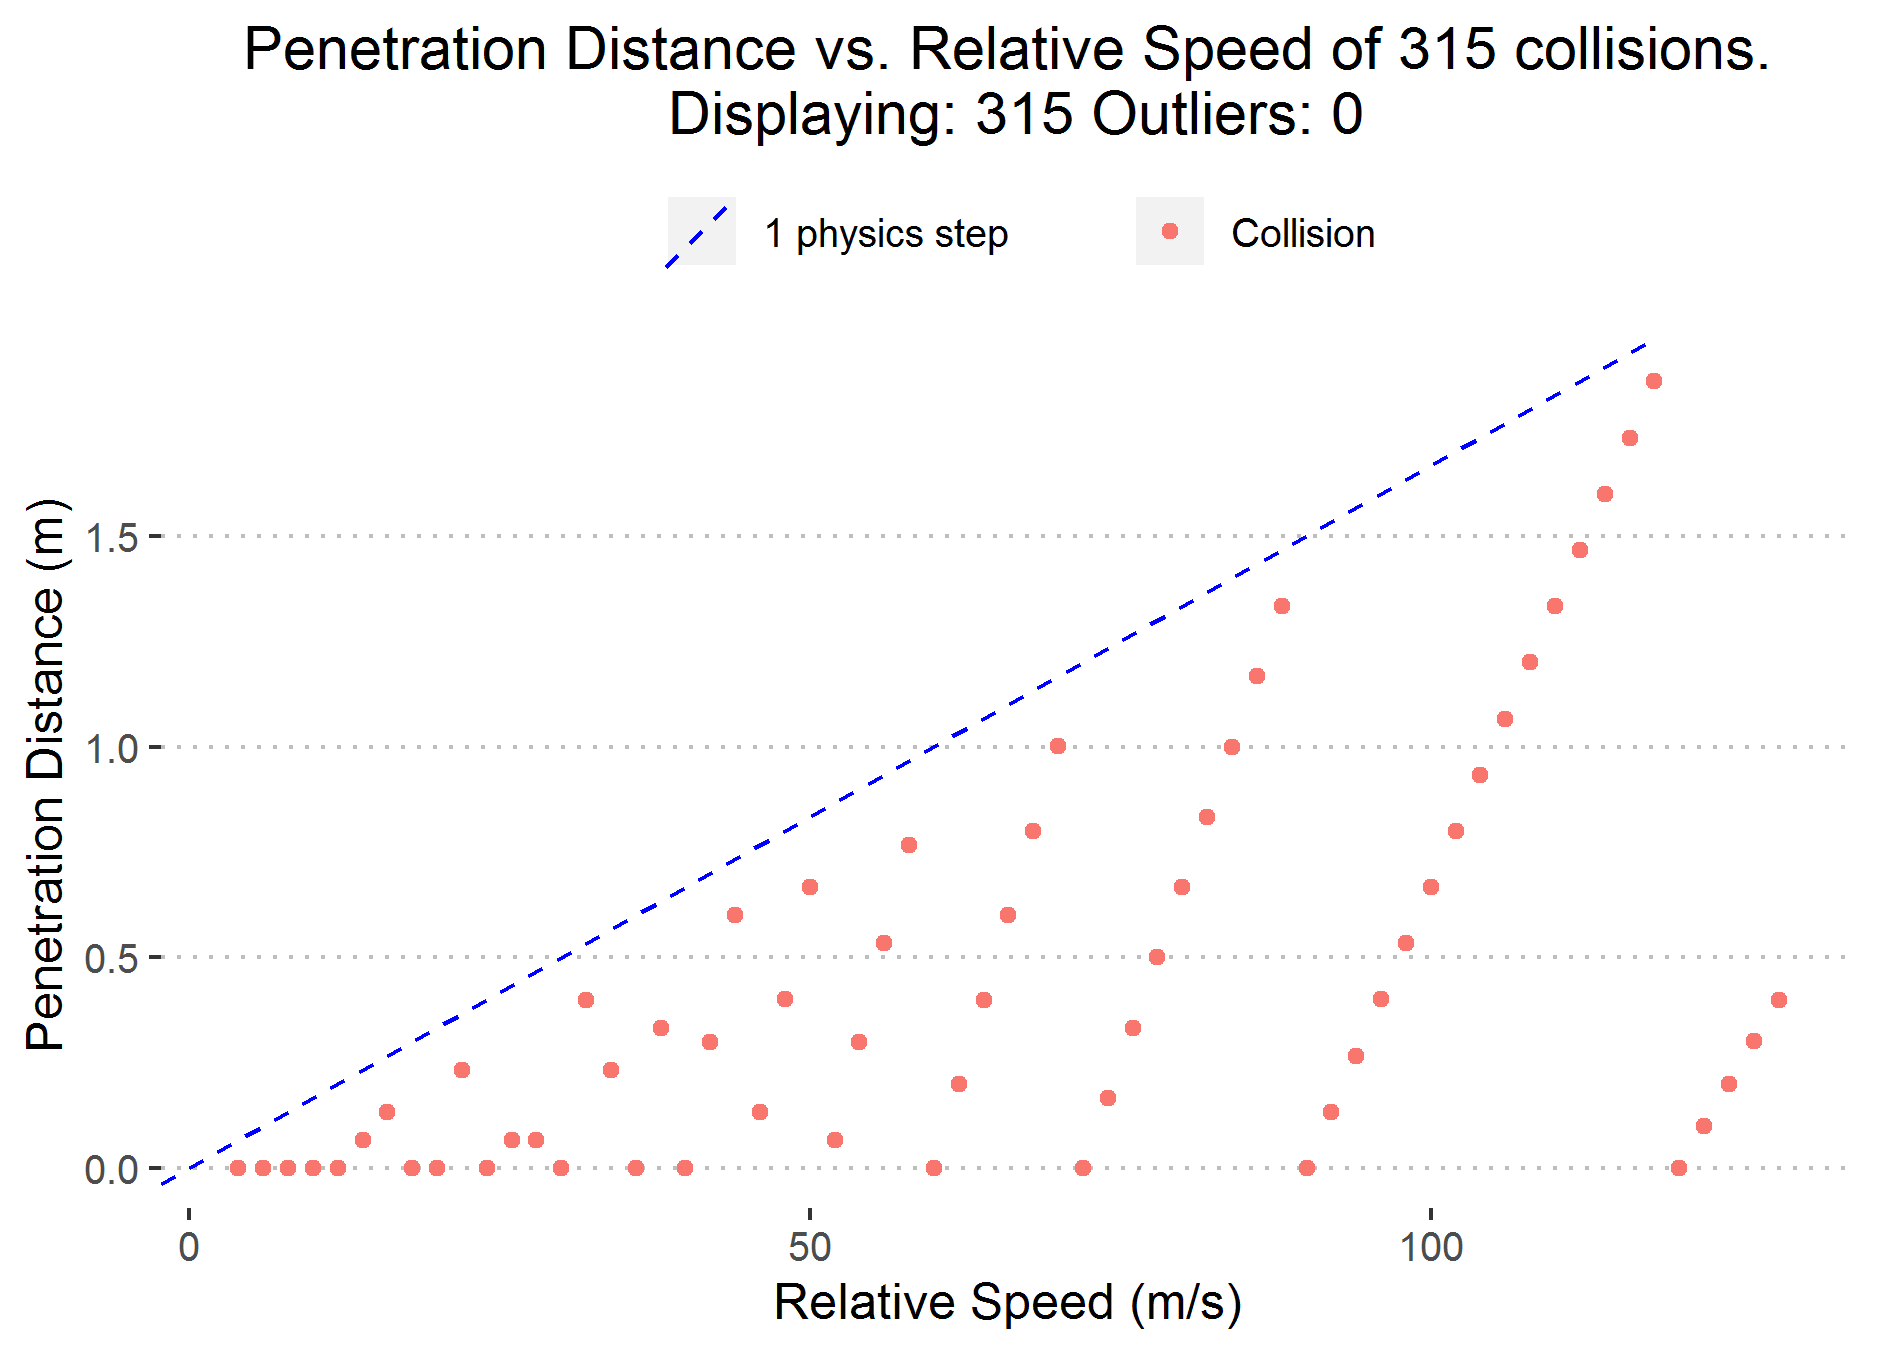
\includegraphics[width=\textwidth]{CentralCollisionsPenDistanceVsSpeed}
%	\caption{Penetration distance of collisions with varying speed. The maximum expected penetration distance of 1 physics step is marked with a dashed blue line.}
%	\label{fig_ErrorControlDistance}
%\end{figure}

\begin{figure}[t]
	\centering
	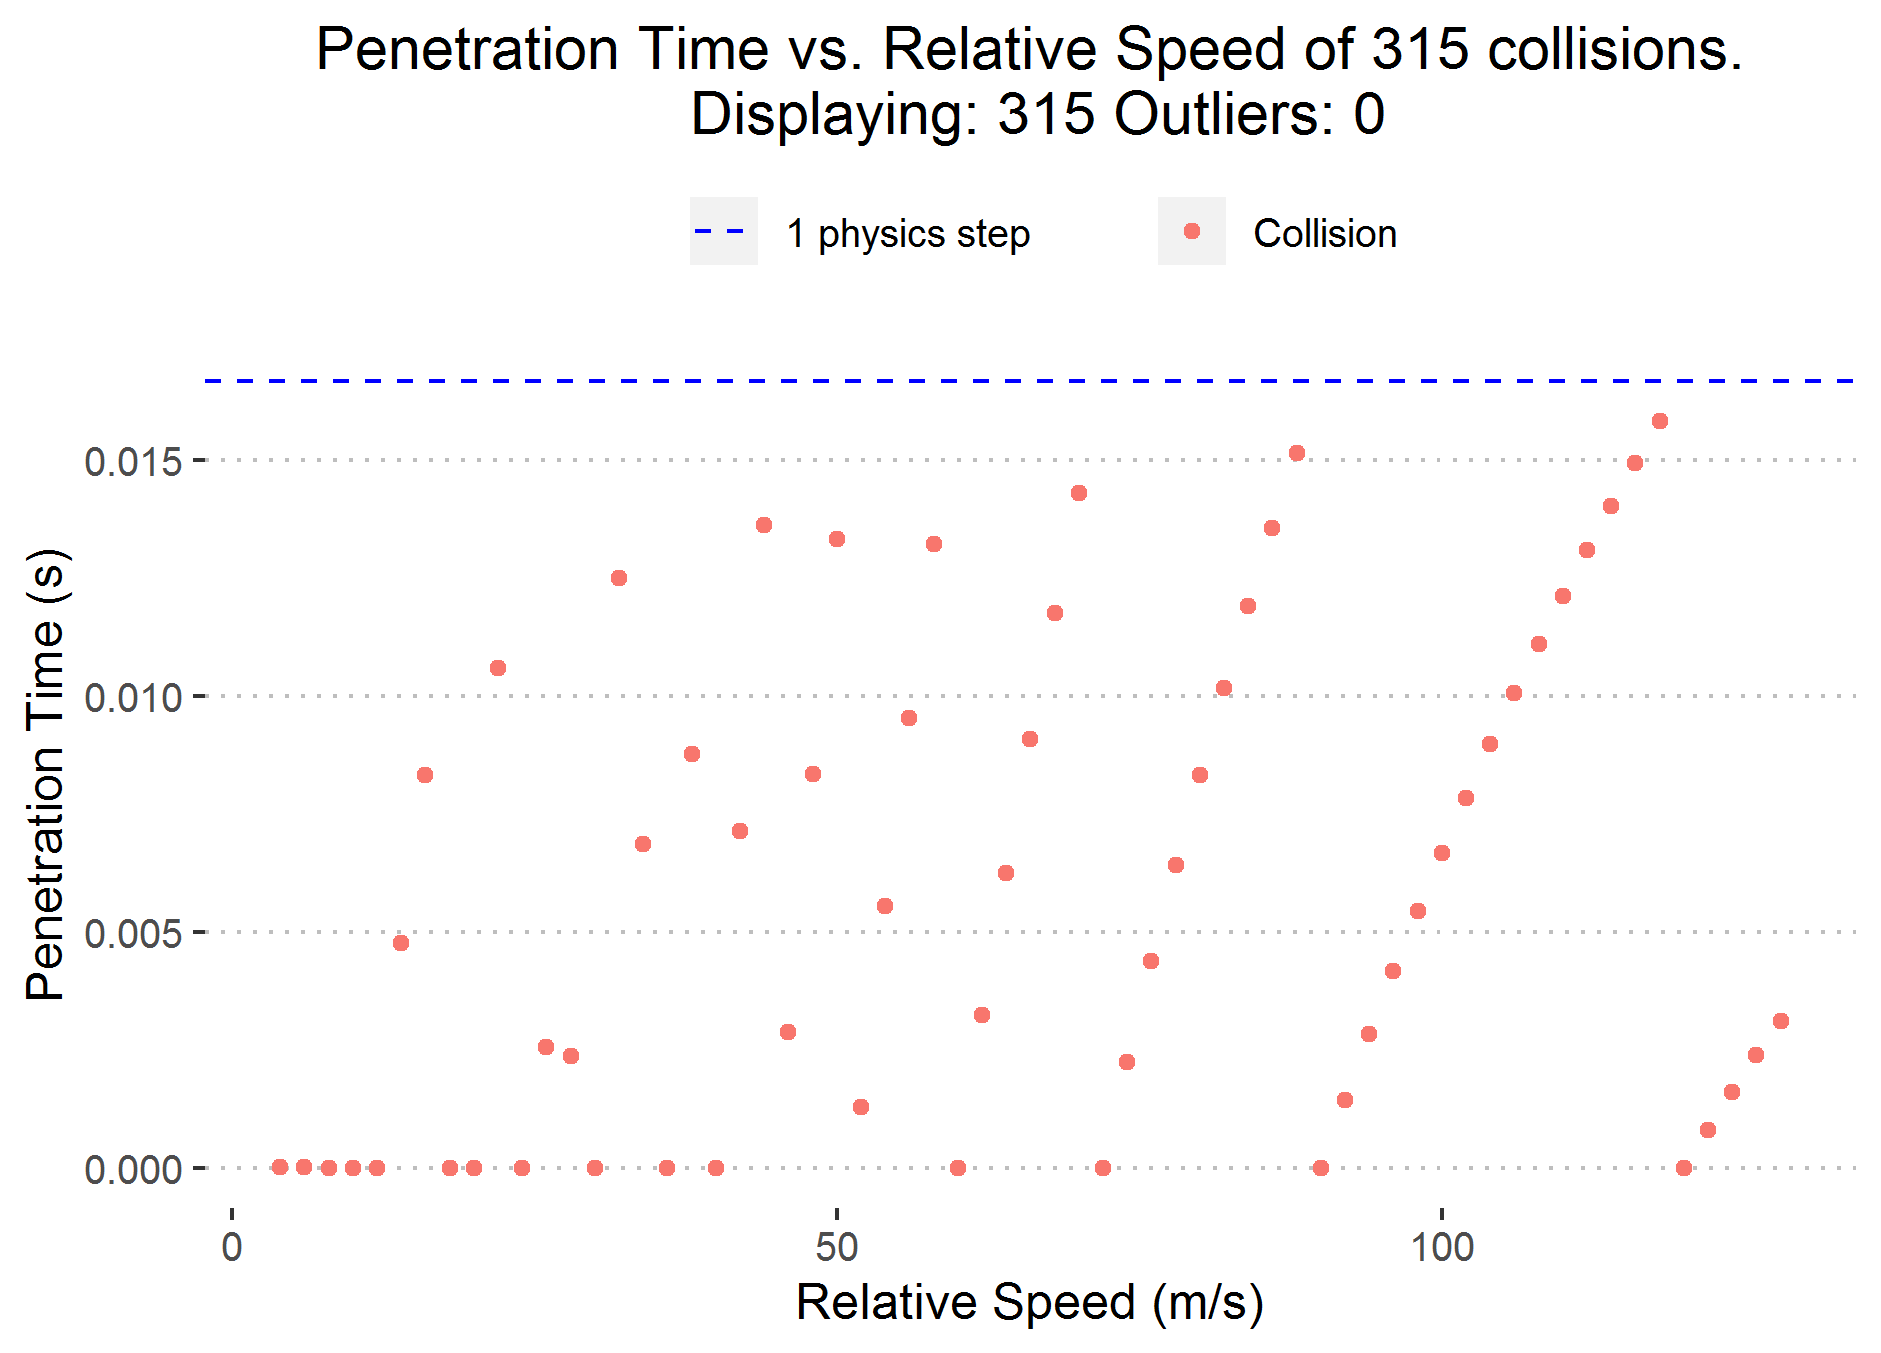
\includegraphics[width=\textwidth]{CentralCollisionsPenVsSpeed}
	\caption{Penetration time of collisions with varying speed. The maximum expected penetration time of 1 physics step is marked with a dashed blue line.}
	\label{fig_ErrorControlTime}
\end{figure}

A control experiment on a centralised system (single server, single simulation) was performed, in which the scenario was repeated multiple times. The speed of each object is increased from $1$ to $64m\mathord{\cdot}s^{-1}$ in steps of $1m\mathord{\cdot}s^{-1}$. The experiment was repeated $50$ times, for a total of $3150$ collisions. %Fig. \ref{fig_ErrorControlDistance} shows the penetration of objects with increasing speed in a centralised simulation and demonstrates that penetration distance is never greater than the maximum expected penetration. 

As speed increases, expected penetration increases. Using penetration time gives us a uniform maximum expected value regardless of speed.
Re-arranging $s=d/t$, to $t=d/s$ and substituting the collision penetration for $d$ and speed for $s$, gives us the penetration time for a collision. It should be noted that because physics engines work in discrete time steps, this time value does not actually reflect the real time the colliding objects were penetrating each other. It should also be noted that PhysX can report collisions before objects intersect, leading to the negative penetration distances shown. Correct collisions result in penetration times of up to 1 physics time step and any collision penetration times over this value are considered erroneous. Fig. \ref{fig_ErrorControlTime} shows the penetration of objects with increasing speed in a centralised simulation (displaying speed without the random variation) and demonstrates that penetration time is never greater than the time of one physics step, regardless of the relative speed of objects. The purpose of this experiment was to confirm the predicted maximum expected penetration in a centralised simulation. This provides a benchmark of correctness to compare with results from experiments using multiple servers.

Using the above method to detect late collisions, experiments on a distributed configuration of a simulation were then performed. Experiments were carried out for both variations in all three aura tolerance factors and packet-loss. Experiments were conducted using AWS G2.2xlarge servers located within the same geographical region. A G2.2xlarge instance uses a 2.60GHz Intel Xeon E5-2670 CPU with 16GB RAM and an NVIDIA GRID K520 (Kepler) GPU running Ubuntu 18.04 LTS.

\subsection{Experiment- Varying Factors}
Experiments were carried out to demonstrate the effects of varying each aura calculation factor on the correctness of collisions between objects. The purpose of these experiments is to demonstrate that collisions in AP are always correct if the three factors that determine aura size remain within respective tolerance, i.e. there are no late or missed collisions. In addition, if the aura calculation is correct, we expect to see late collisions begin to occur as soon as tolerances are exceeded. If errors do not occur as soon as the tolerances are exceeded, this is evidence that the aura radius is too large. Large auras can lead to reduced performance in AP, therefore auras that are only as large as needed to be, for the given tolerance, are desirable to maximise performance.

In order to rigorously test the hypothesis "Can real-time physics simulations remain correct when scaled?", a `worst-case' scenario was used for the experiments, in which two objects are moving directly towards each other and collide while one of the objects is intersecting the boundary between servers. This experiment setup is illustrated in Fig. \ref{fig_CorrectnessExperiment}. In this experiment two servers were used with one sphere being created on each server. The two spheres were given starting positions so the two would collide at a point when one of the spheres is intersecting the server region boundary, thus creating the most likely situation for spheres collide with each other in the first time-step after being migrated; this is necessary as AP can only lead to late or missed collisions when at least one sphere involved in the collision has just migrated (received since the last physics time-step). This is because non-migrating spheres behave the same as spheres in a centralised solution, therefore only collisions that involve a sphere that has just migrated are considered in the experiment results.

\begin{figure}
	\centering
	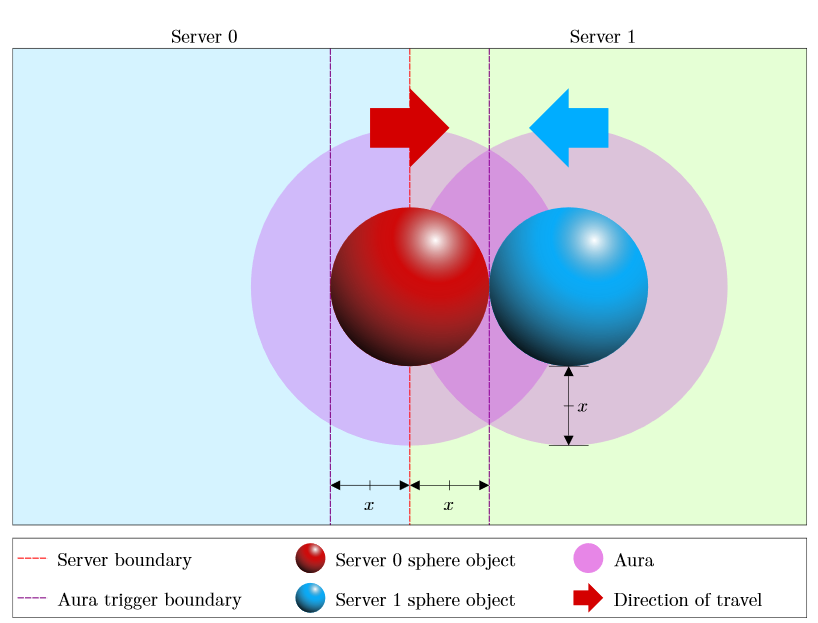
\includegraphics[width=0.9\textwidth]{CorrectnessExperiment}
	\caption{Correctness experiment setup. The setup is the `worst-case' scenario, in which two objects are moving directly towards each other and collide while one of the objects is intersecting the boundary between servers.}
	\label{fig_CorrectnessExperiment}
\end{figure}

There are three factors that are used to determine aura size: speed; latency; and frame-time. In order to demonstrate that collisions always remain correct when within their tolerance, even under worsening conditions and the effect each factor has on collision correctness, one aura factor is varied per experiment and the other two factors are set to equal the tolerance values. For example, speed is varied, the latency between the servers is set to equal the latency tolerance value and the frame-time of each server is set to equal the frame-time tolerance value. The non-varied factors are set to equal the tolerance values as exceeding the tolerance value in one factor can be compensated for by having a value below the tolerance in a different factor. For example, the latency may exceed the tolerance by $5ms$, but the frame-time could be more than $5ms$ below the frame-time tolerance and the collision would still be expected to be correctly handled by AP.

Speed is controlled such that the two objects used in the experiment collide with each other with that desired speed. Latency is controlled using the Traffic Control tool to emulate latency for all communications between the servers. The desired latency is applied as a fixed delay to each server, resulting in that delay being applied to all packets outgoing from that server. Frame-time is controlled using a wait within the simulation's update loop, which is limited to a target frame-time as the resultant frame-times are a normal distribution with the target frame-time as the median. This is illustrated in Fig. \ref{fig_FrameTimeDensity}. As a result of this, half of all frames are expected to be above the target frame-time, which may cause false-positives in detecting late collisions, in the following experiments. However, the following points should be considered: the variance in frame-time is low; longer frames have to occur exactly at the time of messages being exchanged; exceeding one factor can be compensated for by having a low value in another factor. Therefore, false-positives are expected to be rare up until the tolerance value is approached. It should be noted that variance increases with target frame-time, therefore more false-positives should expected with experiments using higher target frame-times.

\begin{figure}
	\centering
	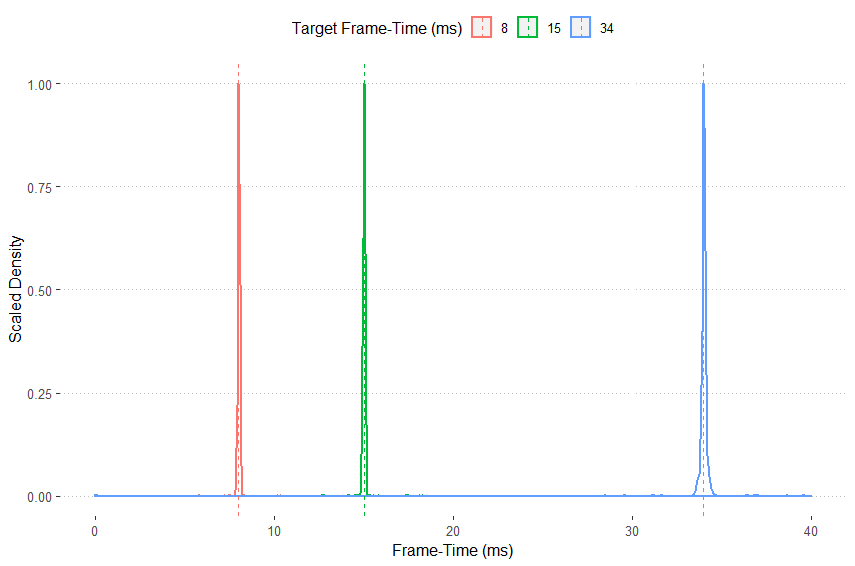
\includegraphics[width=\textwidth]{FrameTimeDensity}
	\caption{Scaled Density of frame-times for the different target frame-times used in the collision correctness experiments. The median of each target frame-time is marked with a vertical dashed line. As target frame-time increases, the distribution of actual frame-time also increases. Frame-time is controlled using a wait within the simulation's update loop, which is limited to a target frame-time as the resultant frame-times are a normal distribution with the target frame-time as the median. As a result of this, half of all frames are expected to be above the target frame-time, which may cause false-positives in detecting late collisions.}
	\label{fig_FrameTimeDensity}
\end{figure}


%The two servers use the same tolerances used in the performance experiments, a maximum speed tolerance of $32m\mathord{\cdot}s^{-1}$, maximum latency tolerance of $2ms$ and a maximum frame-time of $15ms$. Each server has a random delay between $0$ and the target frame-time in order to prevent the two servers always having synchronous update cycles. Each experiment is repeated $10$ times.

For the varying factors experiments, the following parameters were used and output given.
The two servers use the following tolerances unless otherwise stated: a maximum speed tolerance of $32m\mathord{\cdot}s^{-1}$; maximum latency tolerance of $2ms$; and a maximum frame-time tolerance of $15ms$. Each server has a random delay before starting between $0$ and the target frame-time in order to prevent the two servers always having synchronous update cycles. Each experiment is repeated $50$ times. An experiment was conducted for each aura tolerance value. The aura size for the varying tolerances are plotted and the tolerances used are marked. For each experiment, three tolerances values were chosen. For each tolerance value, the following output graphs were plotted:
\begin{itemize}
	\item The ratio of late to correct collisions and ratio of misses to total collision.
	\item The mean and $+/-2$ standard deviations of penetration time were plotted against each tolerance factor for each of the three tolerance values chosen.
\end{itemize}

%For each experiment the following graphs are shown:
%\begin{itemize}
%	\item Collisions, plotting as points with their penetration time against the factor that is being varied along with the maximum expected penetration time and factor tolerance. This shows all the collisions that occurs and illustrates the range of penetration times that the collisions fall within as the factor is varied. %TODO: Mean penetration time
%	\item Mean and Max errors against the varied factor. This includes both the mean error of all collisions, where correct collisions have an error of $0$ and the mean error of just the erroneous collisions. This illustrates how the magnitude of errors change as the factor is varied.
%	\item Ratio of outliers to correct collisions and ratio of misses to total collisions against the varied factor. This illustrates how the number of errors and misses changes as the factor is varied.
%\end{itemize}

%TODO: Also mention very small tolerance for detecting errors, so collisions very close to the line aren't counted as errors. Have to account for floating-point errors throughout the results process.

The first experiment conducted was the varying speed experiment. In this experiment the speed of each of the two objects was varied from $1m\mathord{\cdot}s^{-1}$ to double the the following tolerances: $16m\mathord{\cdot}s^{-1}$; $32m\mathord{\cdot}s^{-1}$ and $48m\mathord{\cdot}s^{-1}$. Increments of $1m\mathord{\cdot}s^{-1}$ were used and the whole experiment repeated $50$ times.

\begin{figure}
	\centering
	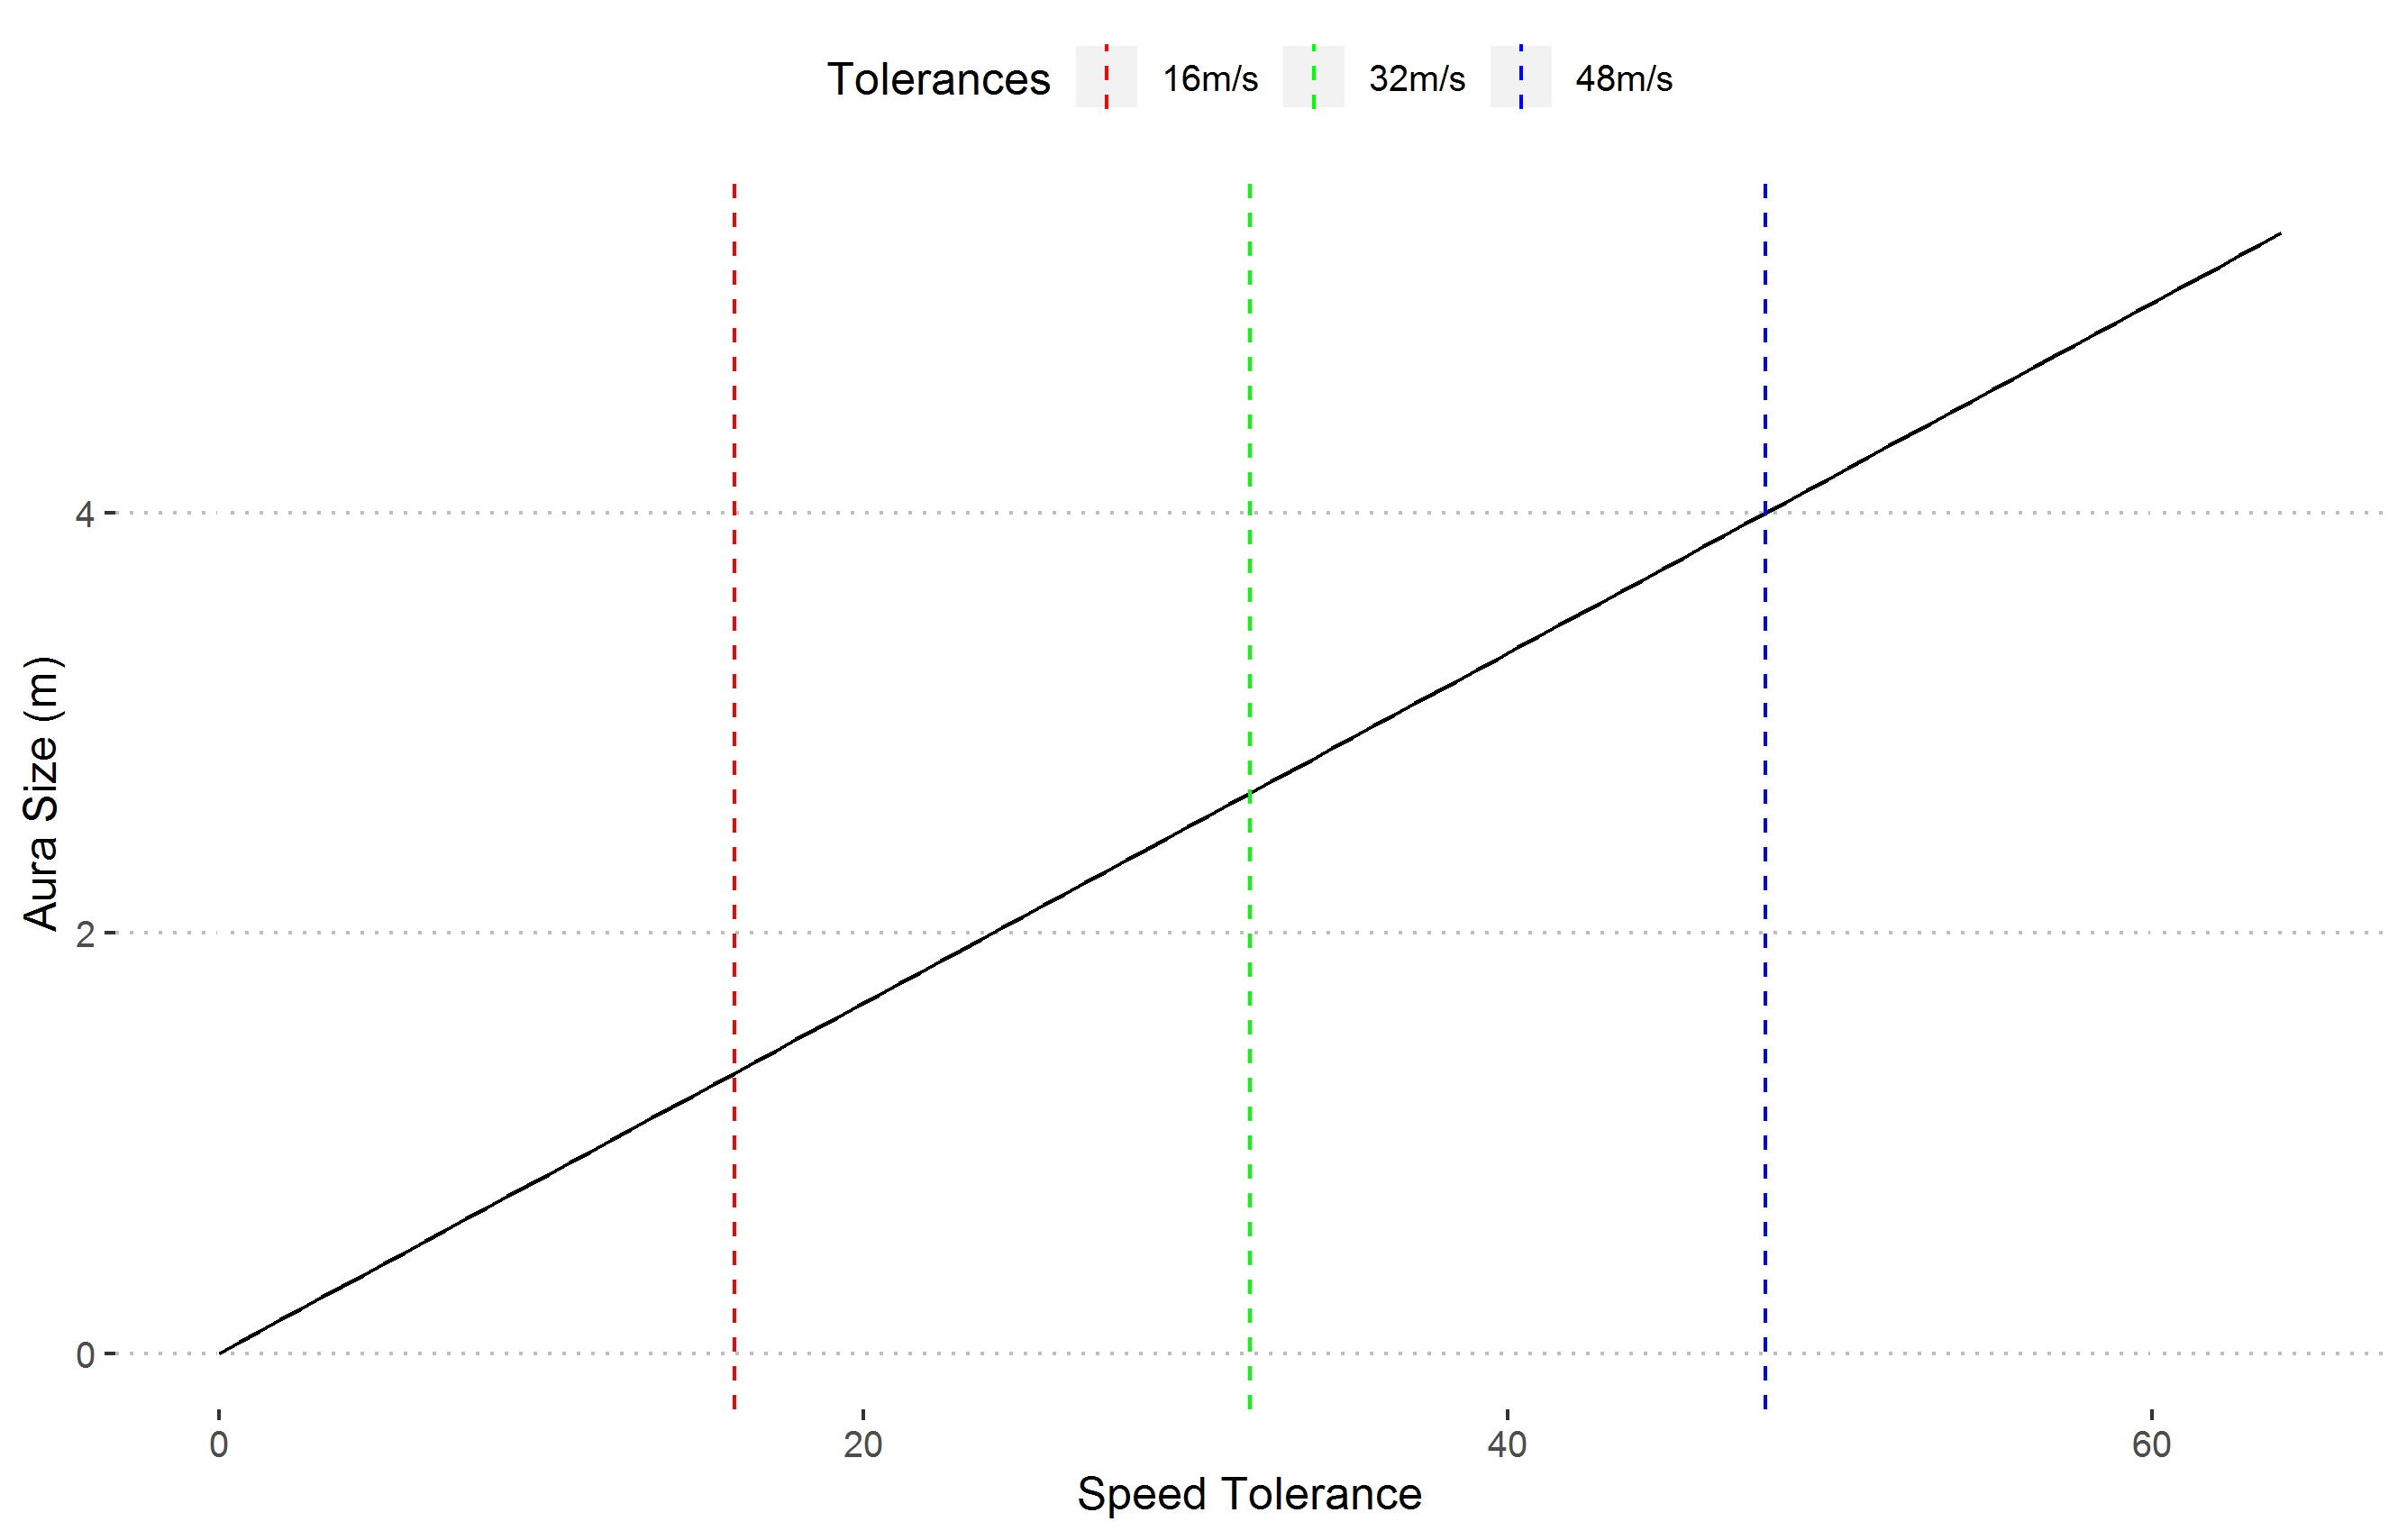
\includegraphics[width=\textwidth]{SpeedAuraSizes}
	\caption{Size of aura vs. speed tolerance. The speed tolerances used are marked in dashed lines}
	\label{fig_SpeedAuraSize}
\end{figure}

Fig. \ref{fig_SpeedAuraSize} shows the size of the aura (not including the bounding sphere of the object) vs increasing speed tolerance, calculated using equation \ref{auraEquation}.
The aura size increases continuously with speed, therefore we expect late collisions to begin immediately once the the speed tolerance is exceeded. False-positives are expected due to the frame-time delay method and should increase as speed increases.

\begin{figure}
	\centering
	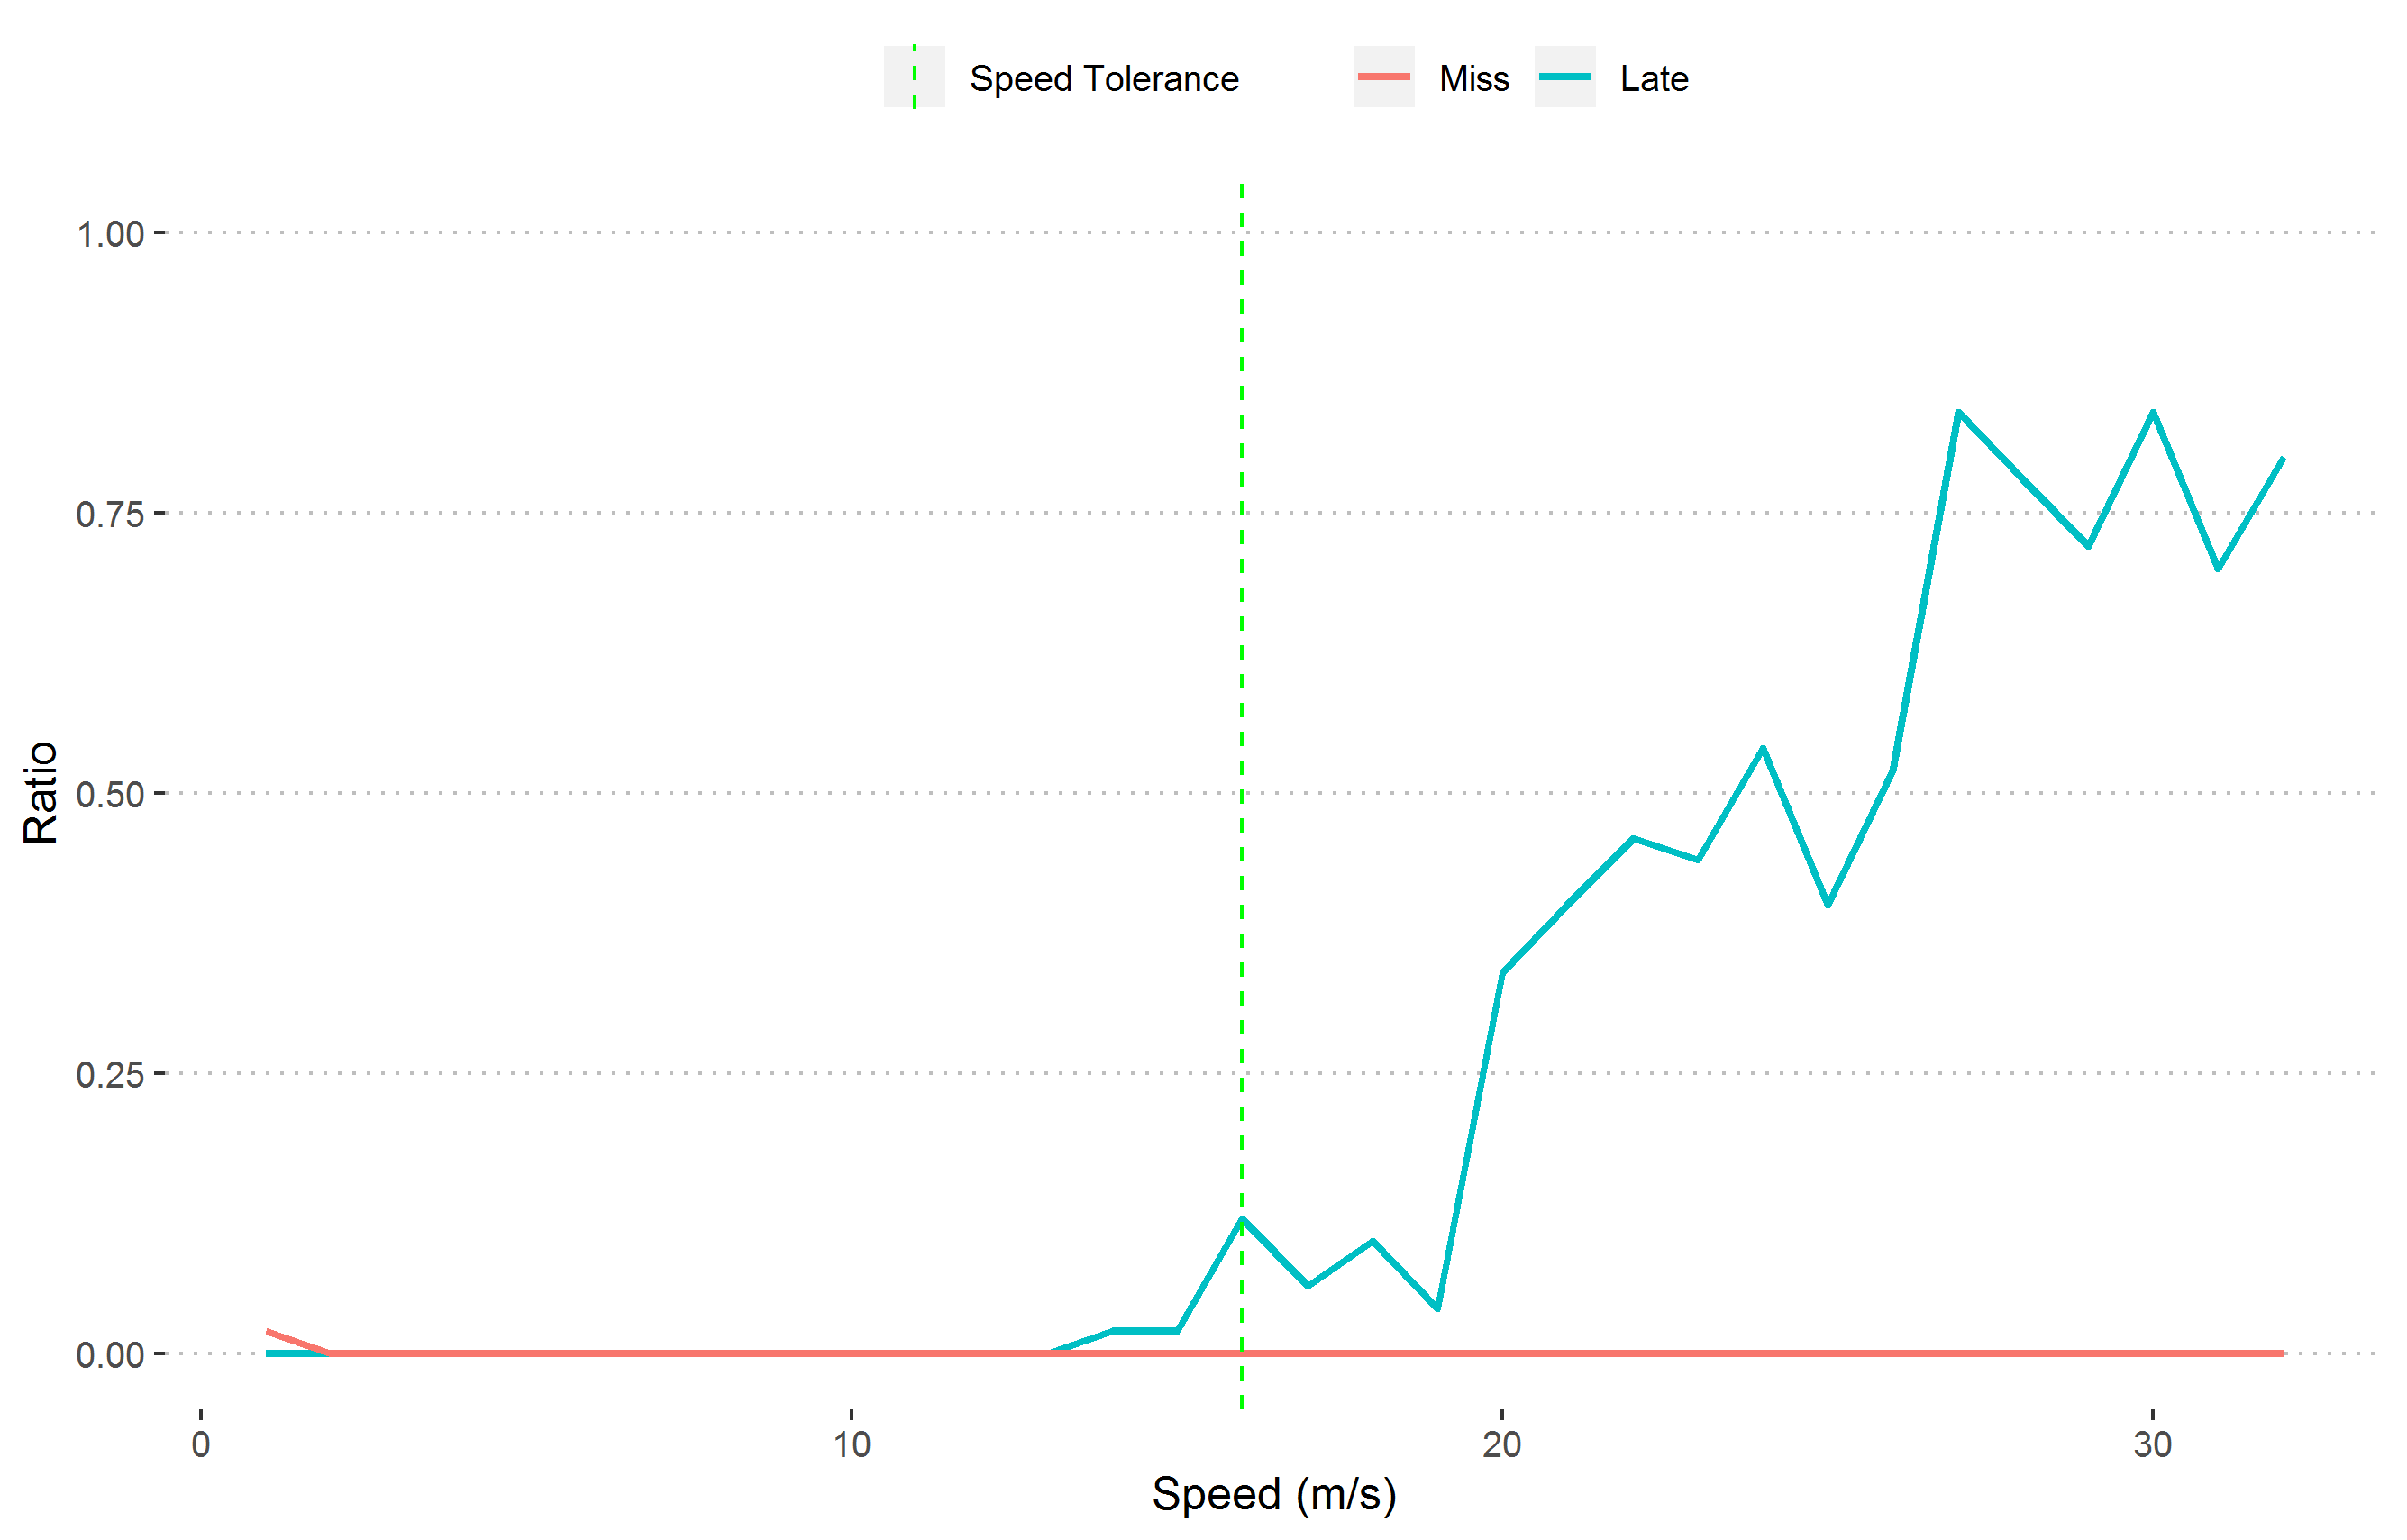
\includegraphics[width=\textwidth]{RatiosVsSpeedLow}
	\caption{Ratio of Late to Correct Collisions and Misses to Total Collision vs. Speed using a speed tolerance of $16m\mathord{\cdot}s^{-1}$. The speed tolerance is marked in a dashed green line.}
	\label{fig_RatioVsSpeedLow}
\end{figure}
\begin{figure}
	\centering
	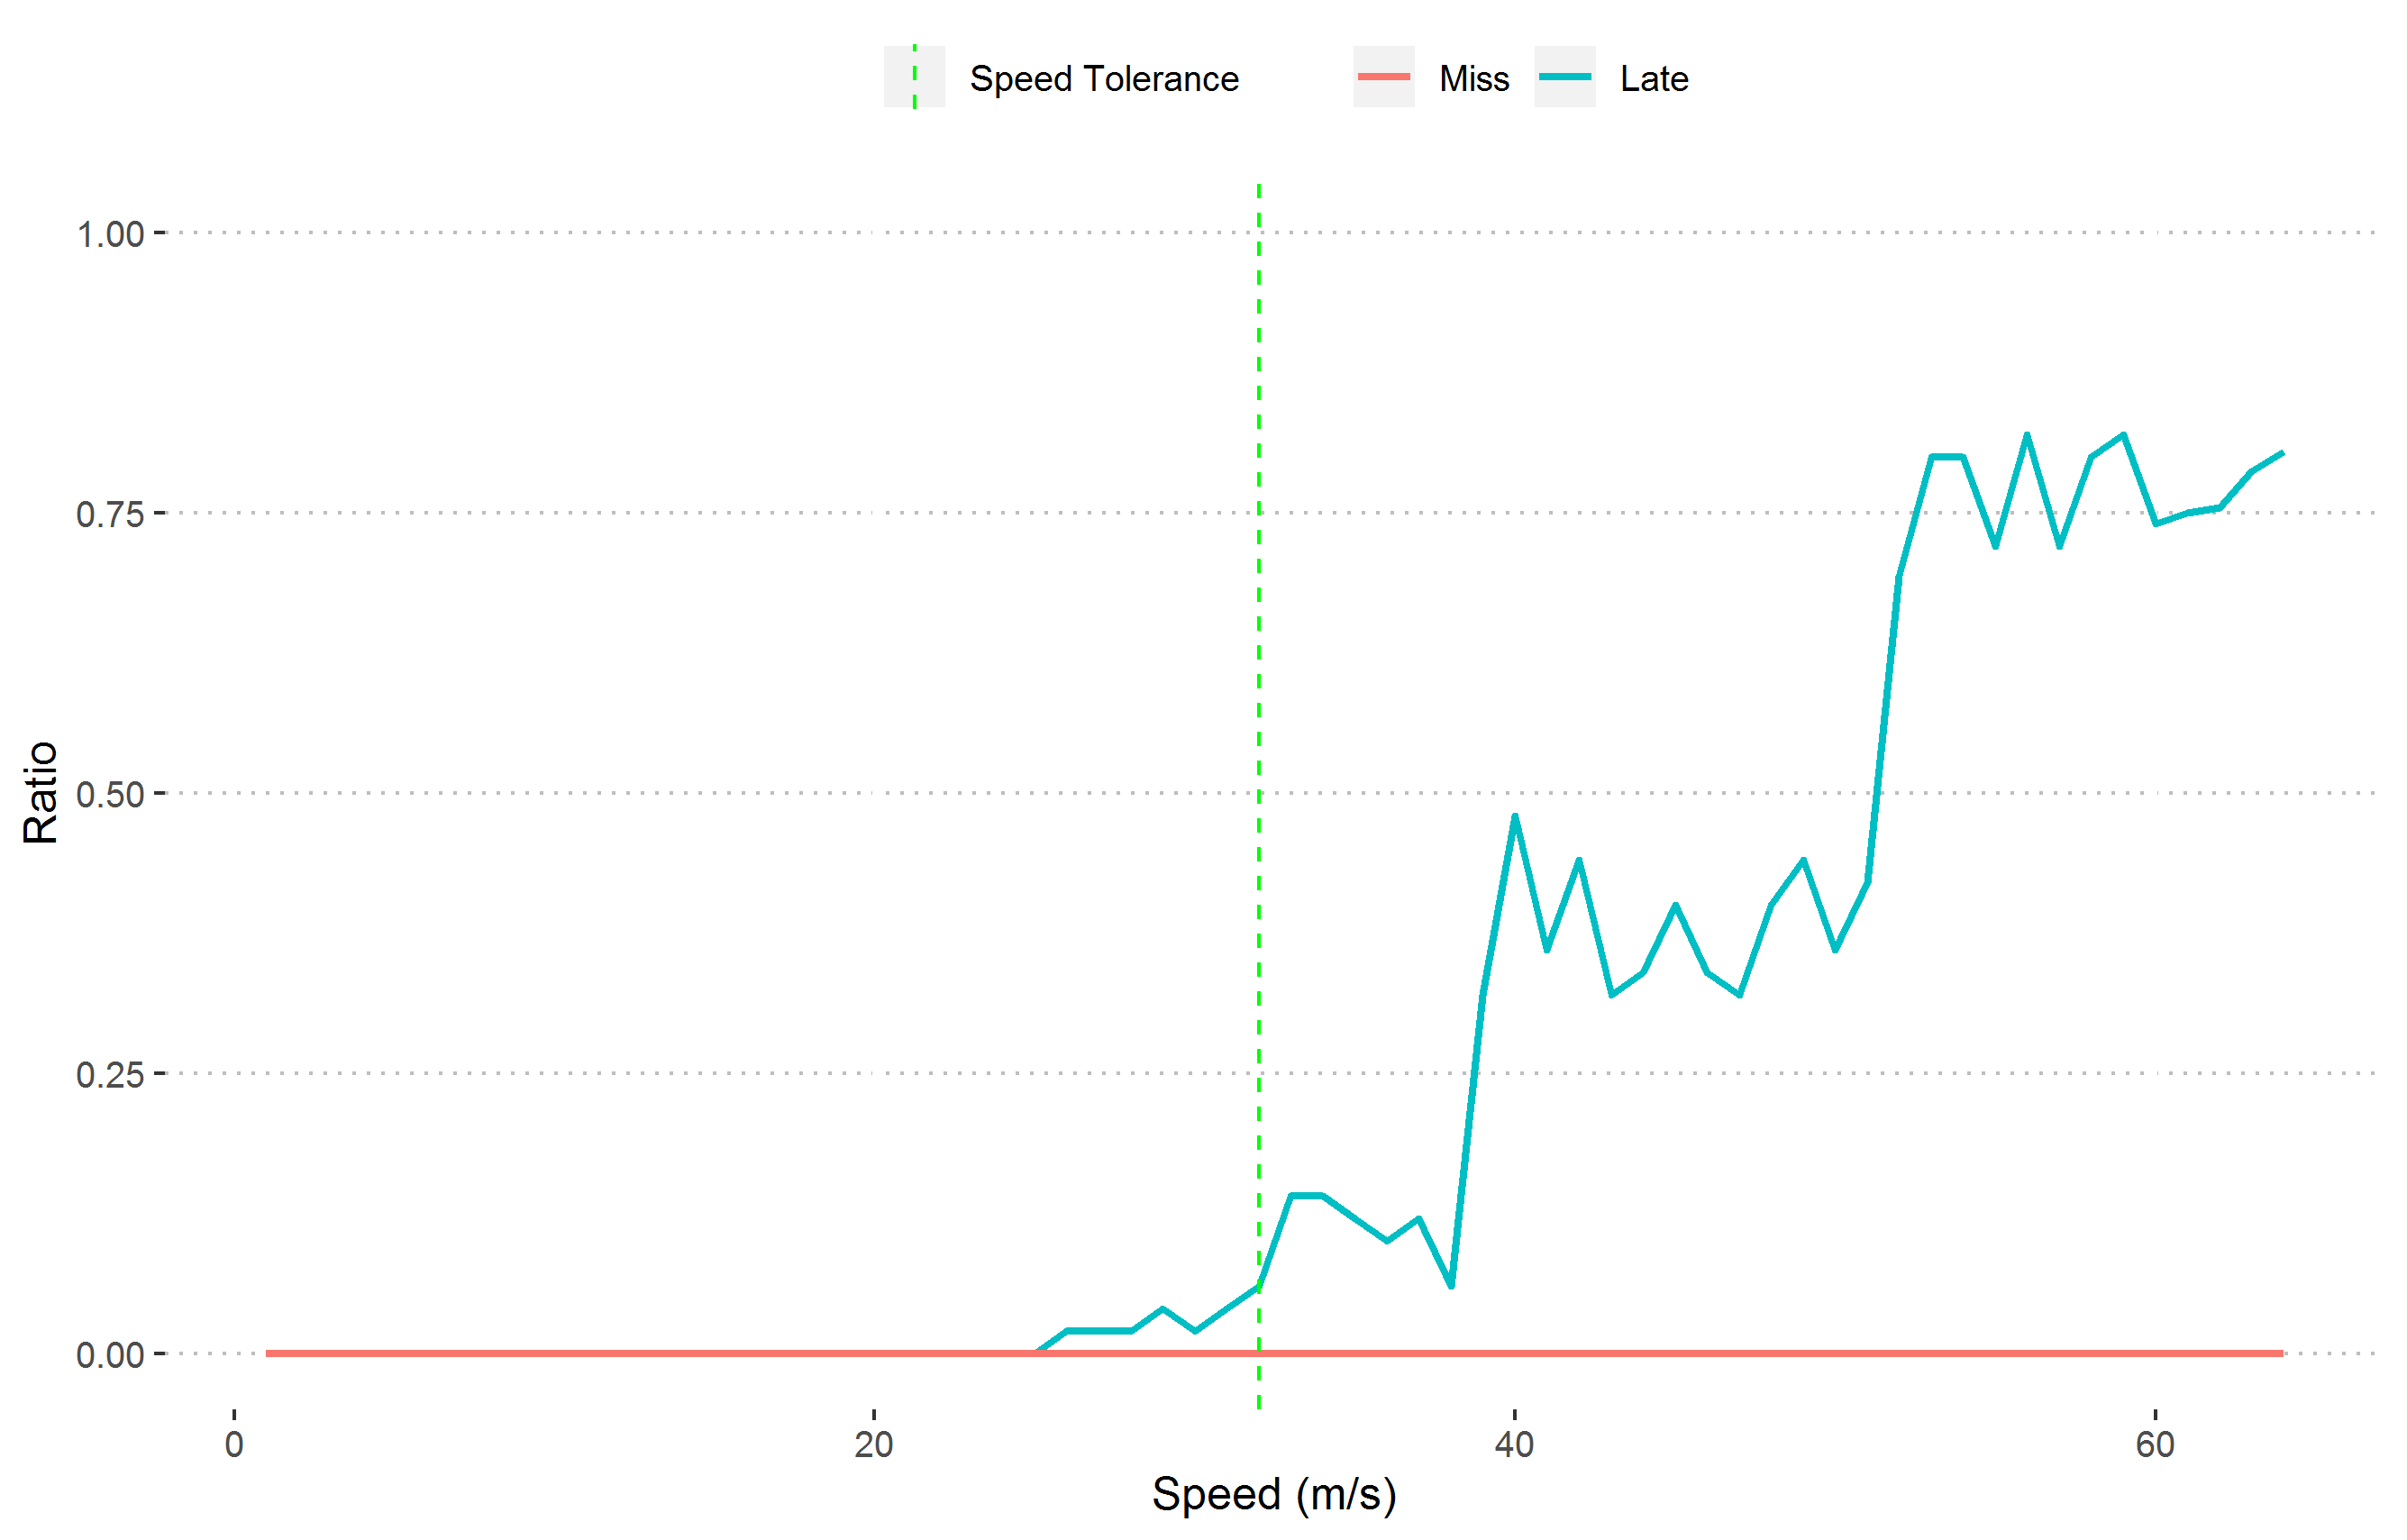
\includegraphics[width=\textwidth]{RatiosVsSpeedMid}
	\caption{Ratio of Late to Correct Collisions and Misses to Total Collision vs. Speed using a speed tolerance of $32m\mathord{\cdot}s^{-1}$. The speed tolerance is marked in a dashed green line.}
	\label{fig_RatioVsSpeedMid}
\end{figure}
\begin{figure}
	\centering
	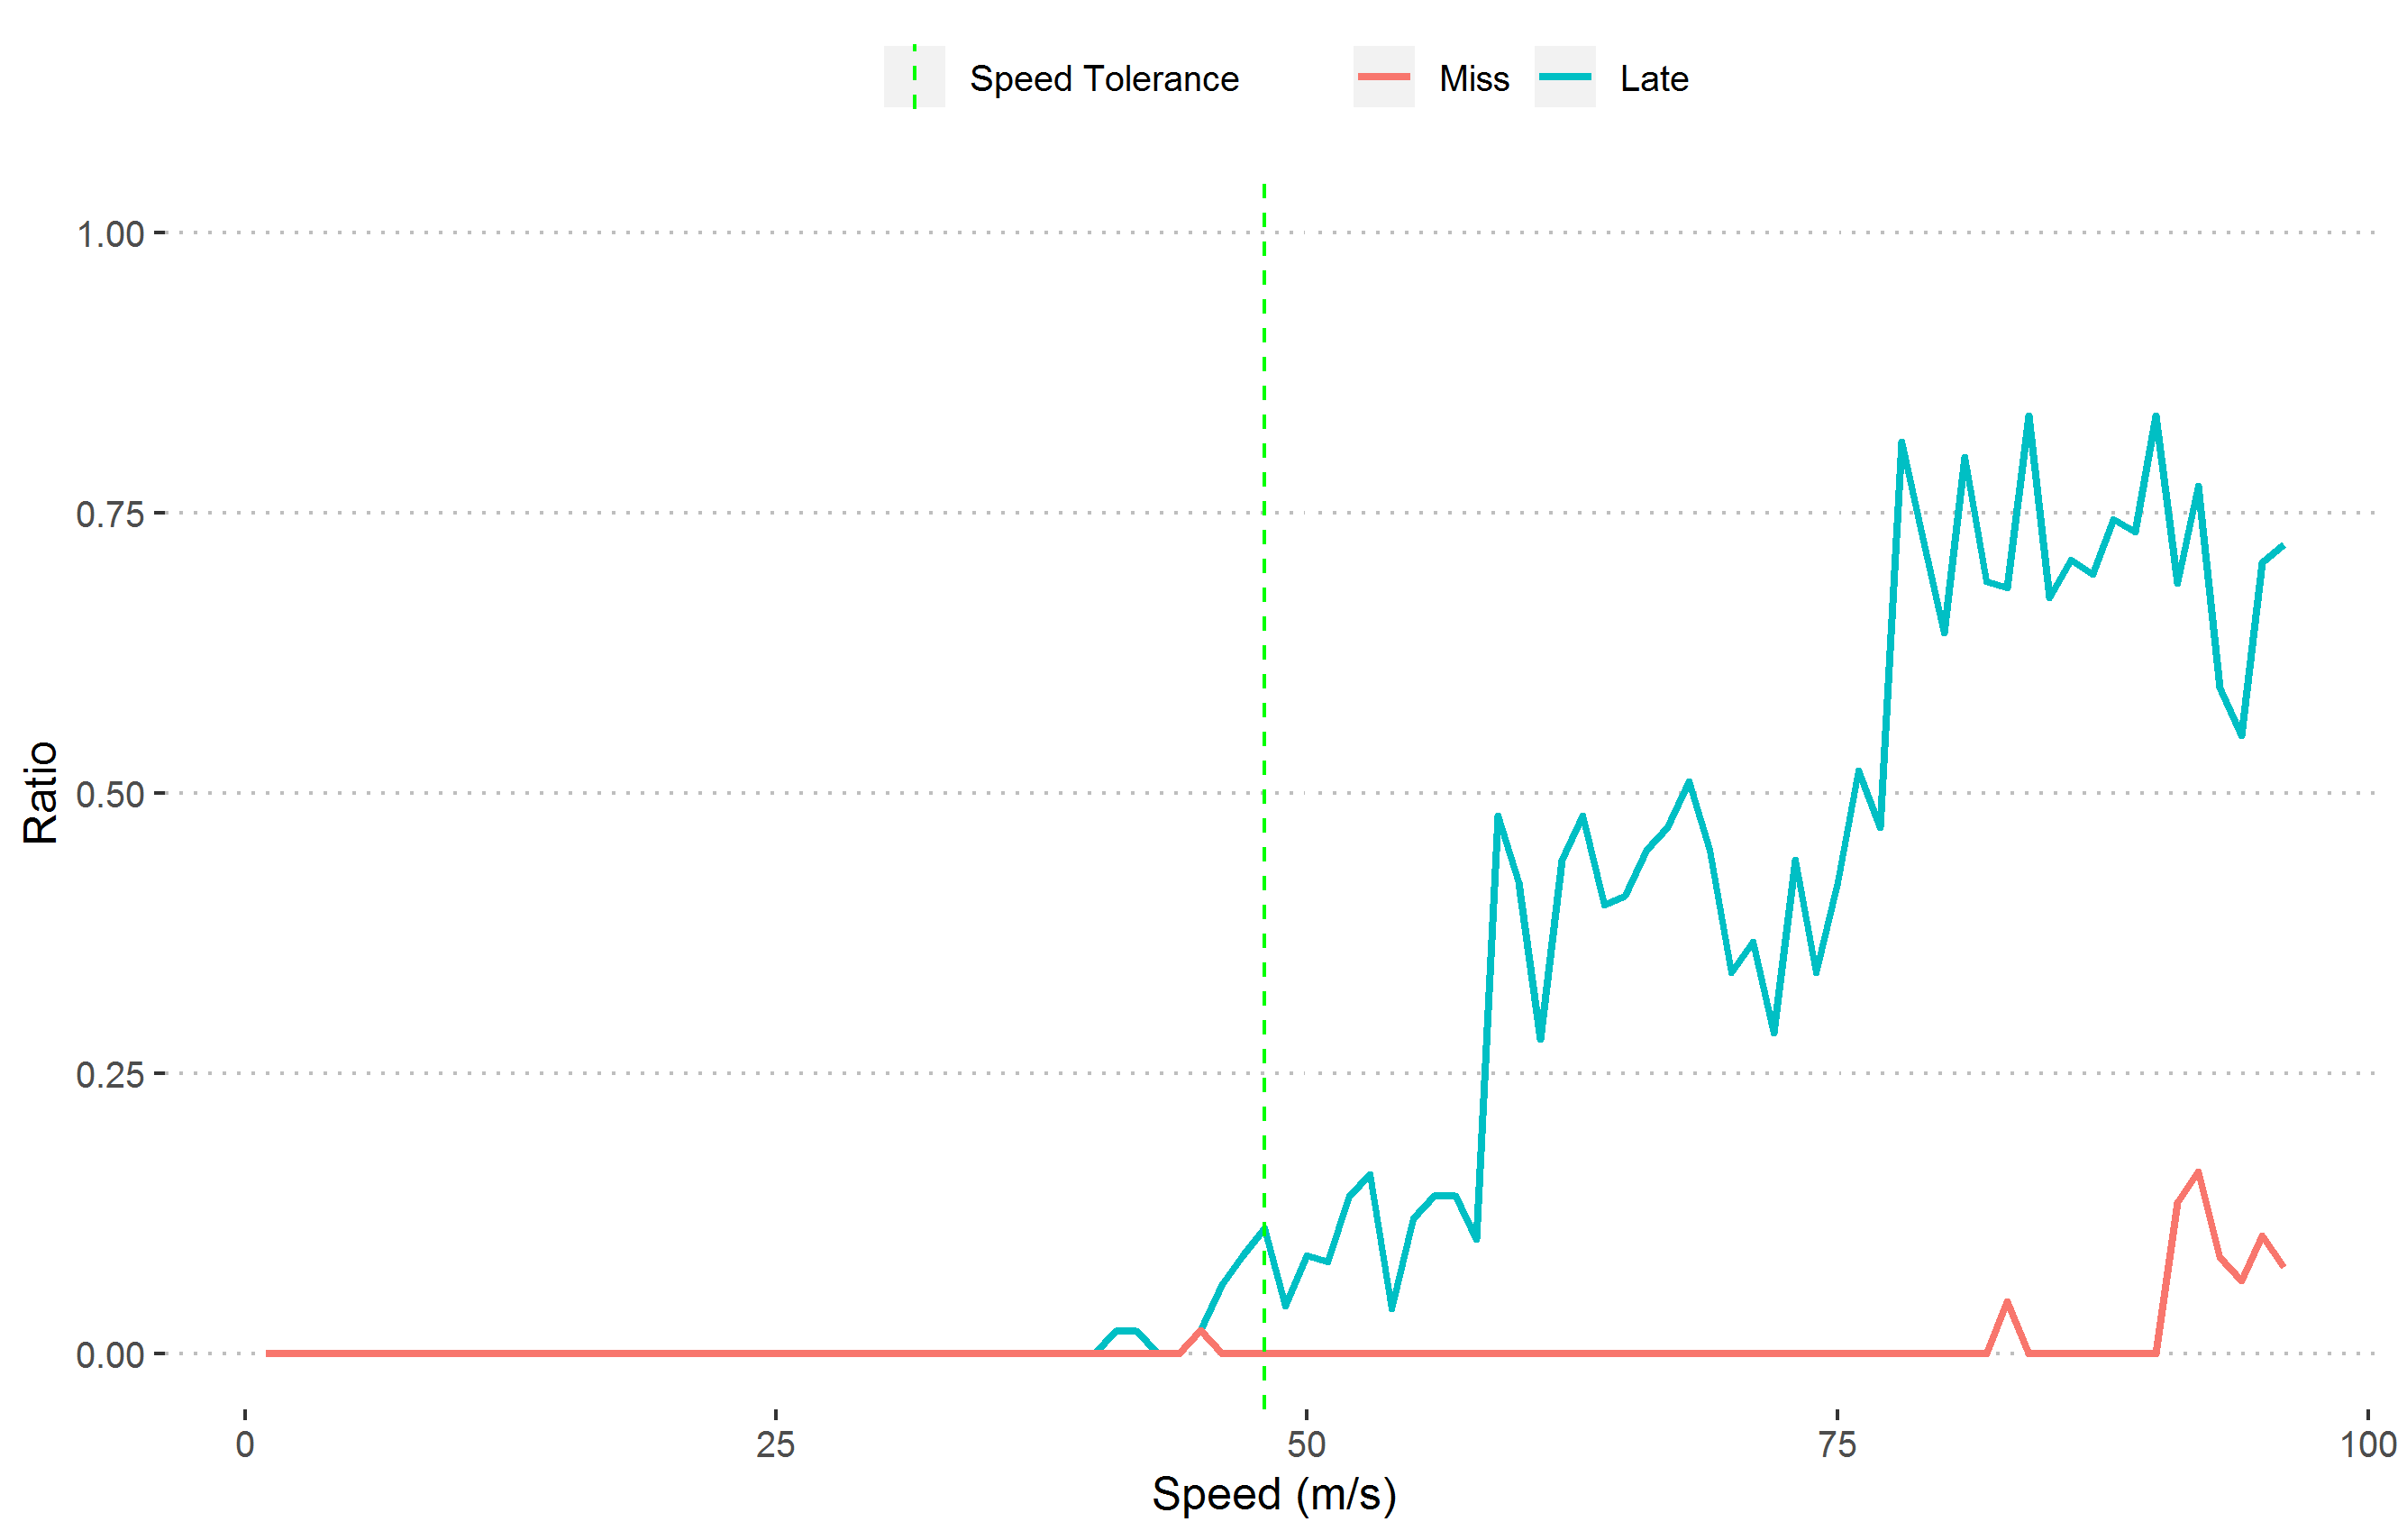
\includegraphics[width=\textwidth]{RatiosVsSpeedHigh}
	\caption{Ratio of Late to Correct Collisions and Misses to Total Collision vs. Speed using a speed tolerance of $48m\mathord{\cdot}s^{-1}$. The speed tolerance is marked in a dashed green line.}
	\label{fig_RatioVsSpeedHigh}
\end{figure}

\begin{figure}
	\centering
	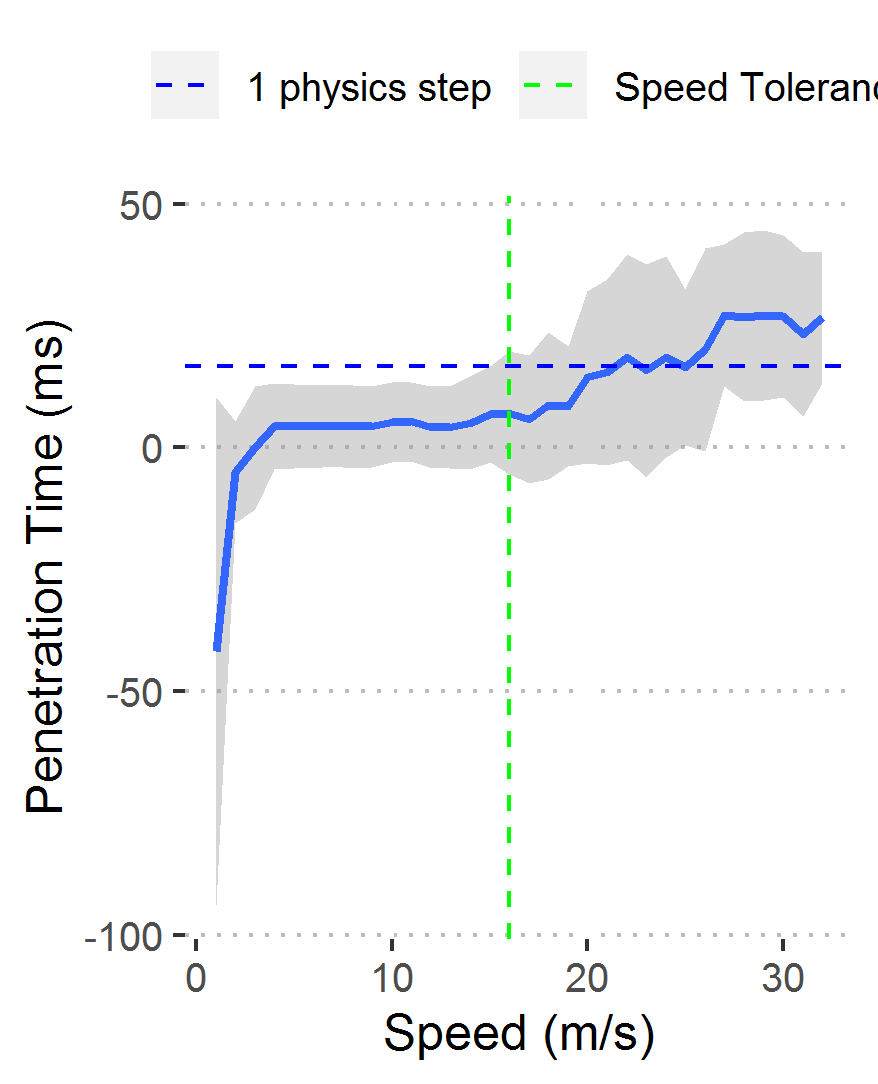
\includegraphics[width=\textwidth]{MeanPenVsSpeedLow}
	\caption{Mean penetration time of objects with $+/-2$ standard deviations with varying speed using a speed tolerance of $16m\mathord{\cdot}s^{-1}$. The maximum expected penetration time of 1 physics step is marked with a dashed blue line. The speed tolerance is marked in a dashed green line.}
	\label{fig_CollisionsPenVsSpeedLow}
\end{figure}
\begin{figure}
	\centering
	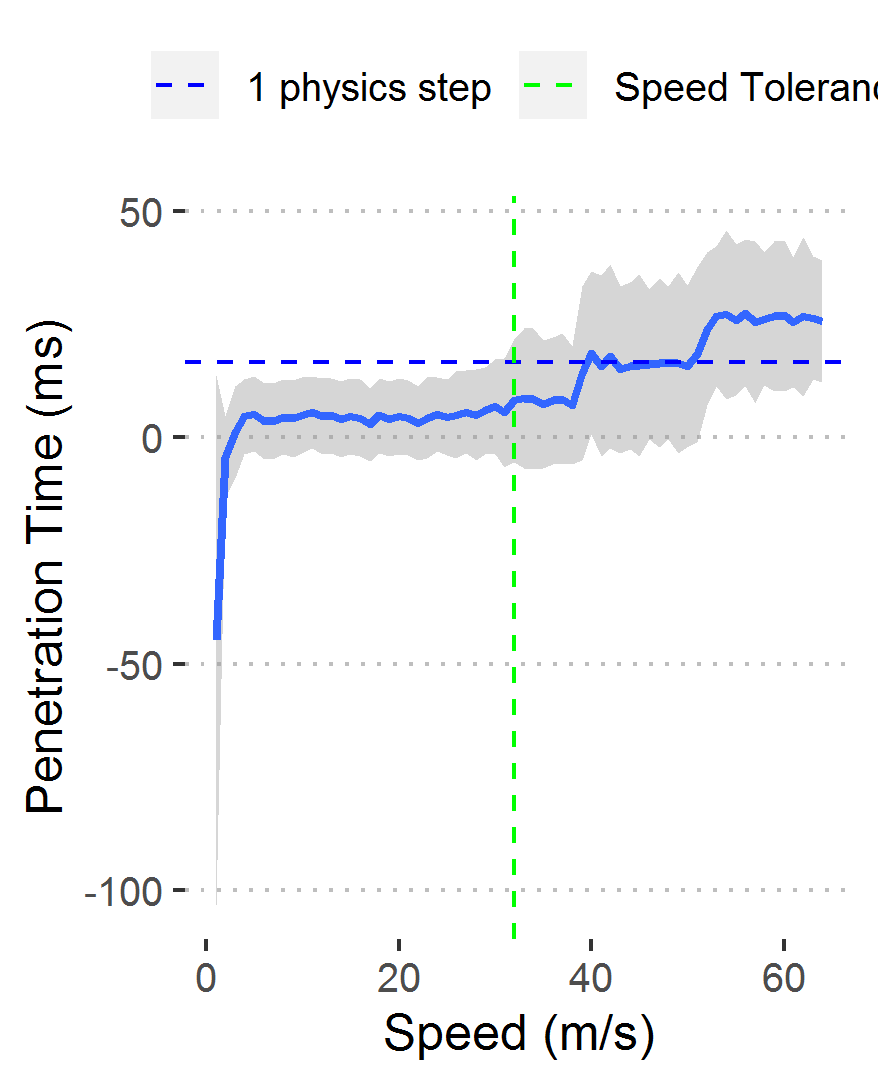
\includegraphics[width=\textwidth]{MeanPenVsSpeedMid}
	\caption{Mean penetration time of objects with $+/-2$ standard deviations with varying speed using a speed tolerance of $32m\mathord{\cdot}s^{-1}$. The maximum expected penetration time of 1 physics step is marked with a dashed blue line. The speed tolerance is marked in a dashed green line.}
	\label{fig_CollisionsPenVsSpeedMid}
\end{figure}
\begin{figure}
	\centering
	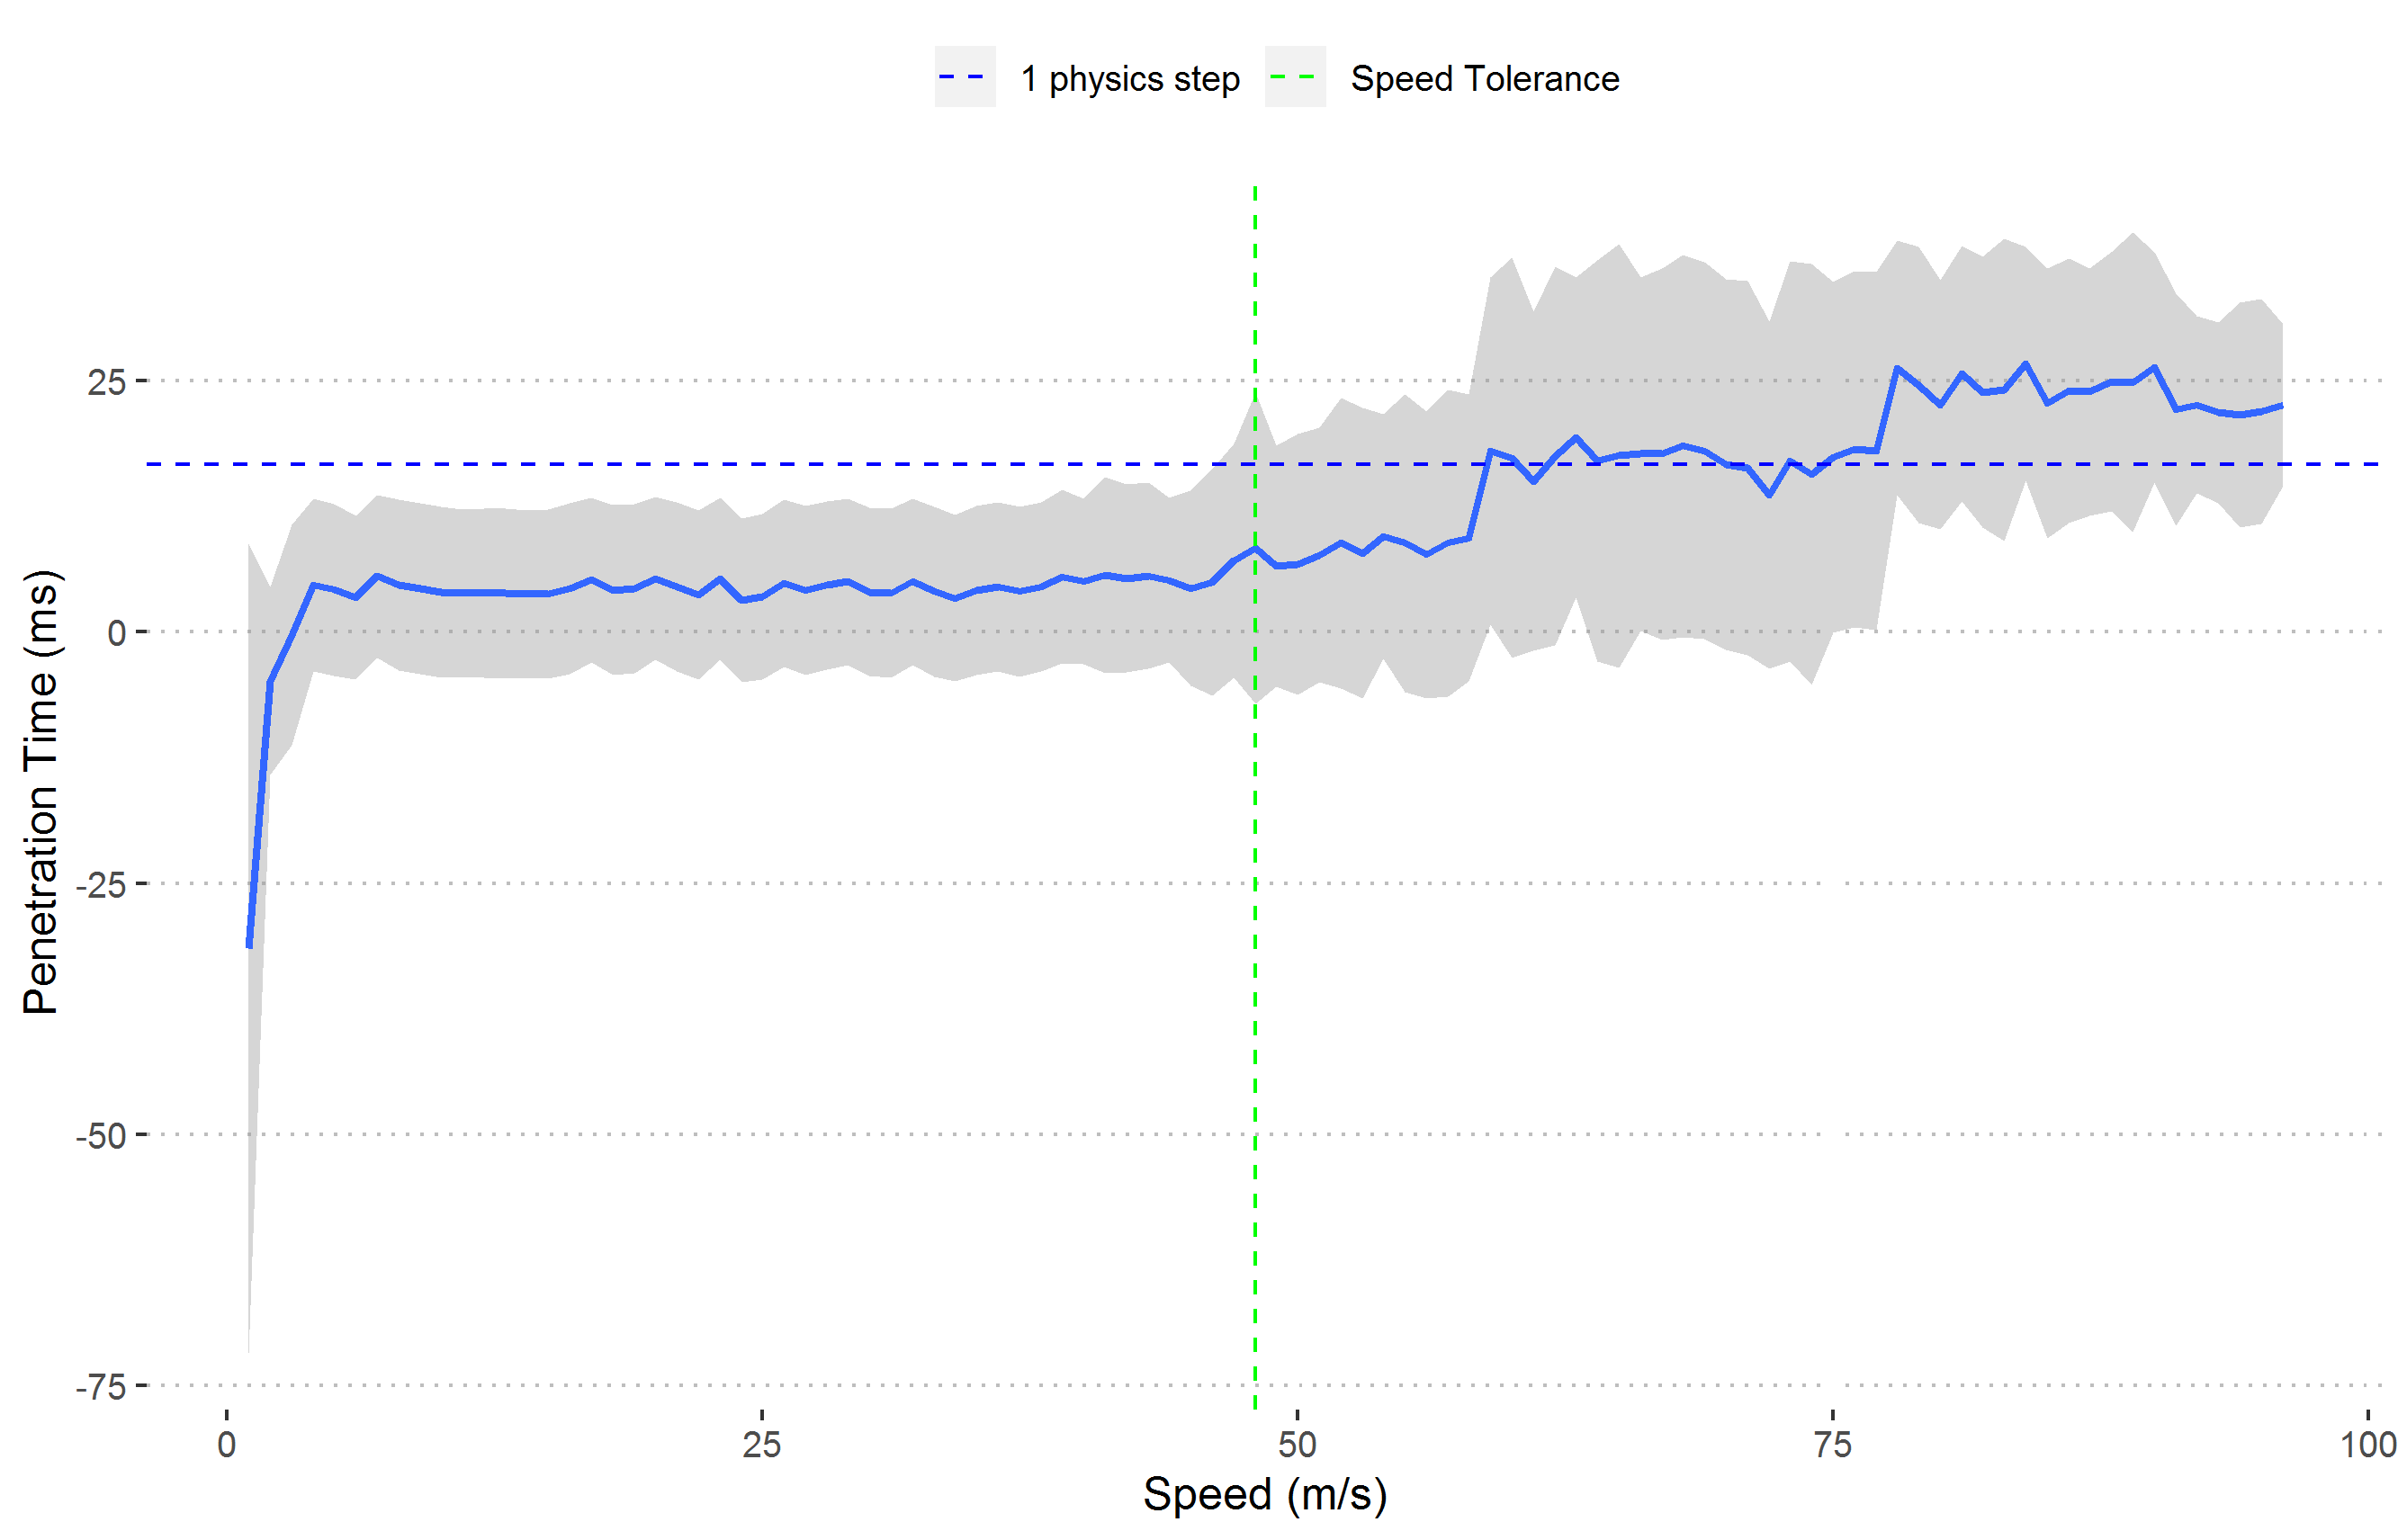
\includegraphics[width=\textwidth]{MeanPenVsSpeedHigh}
	\caption{Mean penetration time of objects with $+/-2$ standard deviations with varying speed using a speed tolerance of $48m\mathord{\cdot}s^{-1}$. The maximum expected penetration time of 1 physics step is marked with a dashed blue line. The speed tolerance is marked in a dashed green line.}
	\label{fig_CollisionsPenVsSpeedHigh}
\end{figure}
	%\label{fig_CollisionsPenVsSpeed}
%\begin{figure}
%	\centering
%	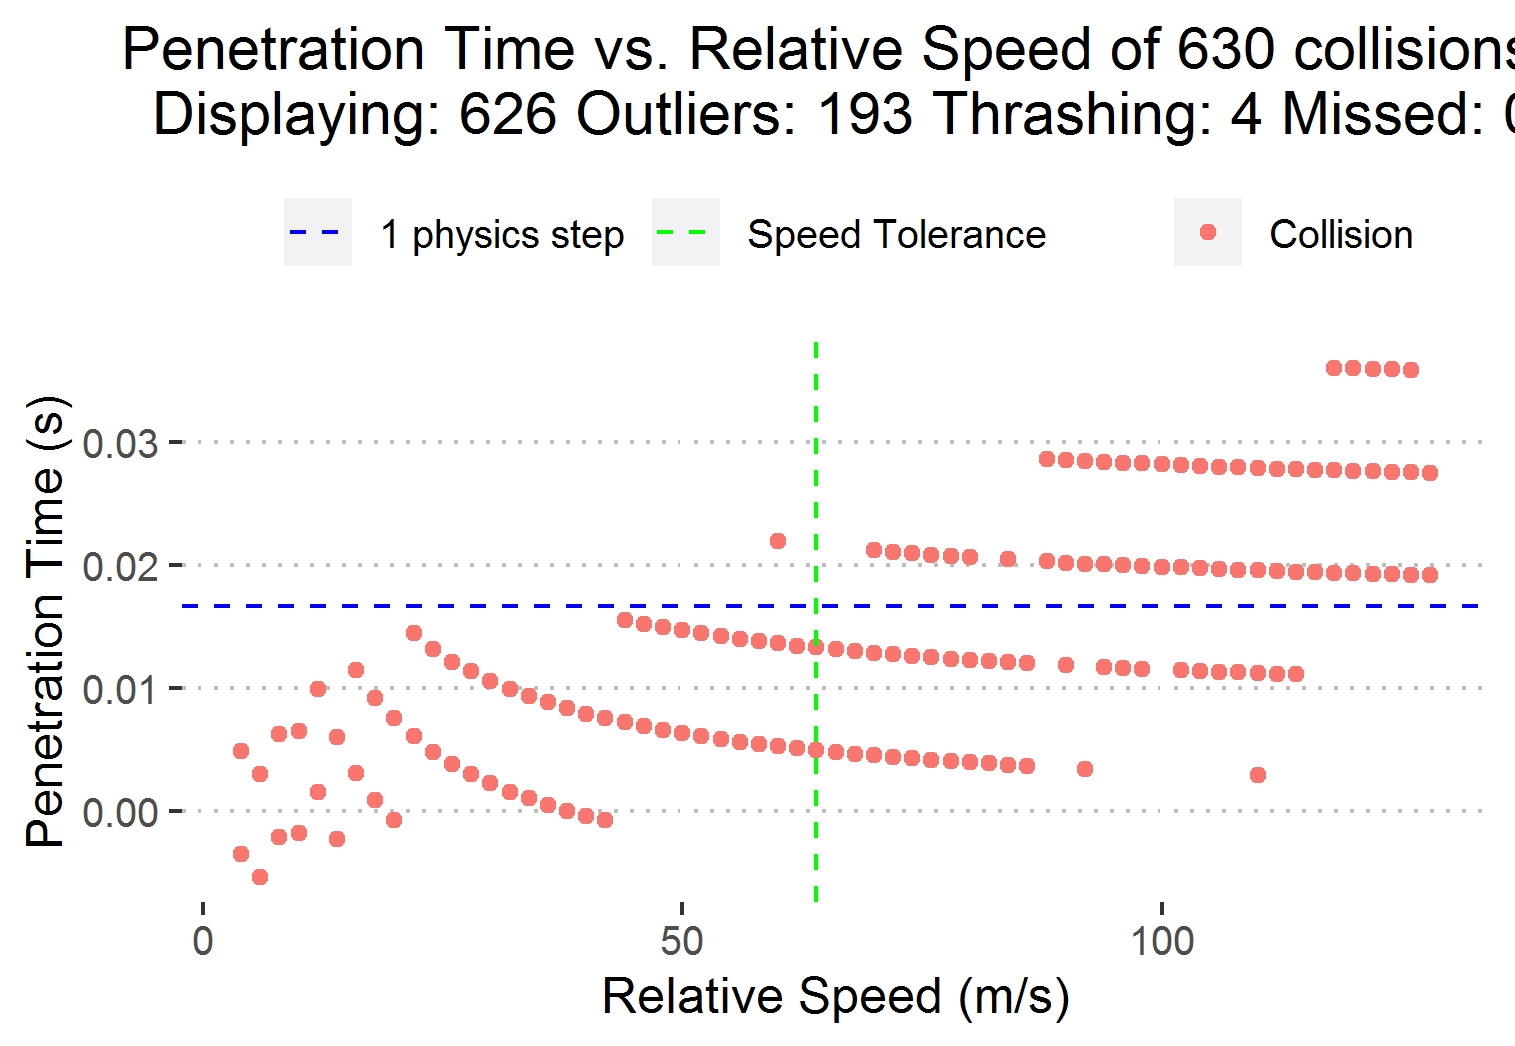
\includegraphics[width=\textwidth]{CollisionsPenVsSpeed}
%	\caption{Penetration time of objects with varying relative speed. Each red point represents one or more collisions. The maximum expected penetration time of 1 physics steps is marked with a dashed blue line. The speed tolerance is marked in a dashed green line. The number and magnitude of errors increases as relative speed increases beyond the tolerance.}
%	\label{fig_CollisionsPenVsSpeed}
%\end{figure}
%
%\begin{figure}
%\centering
%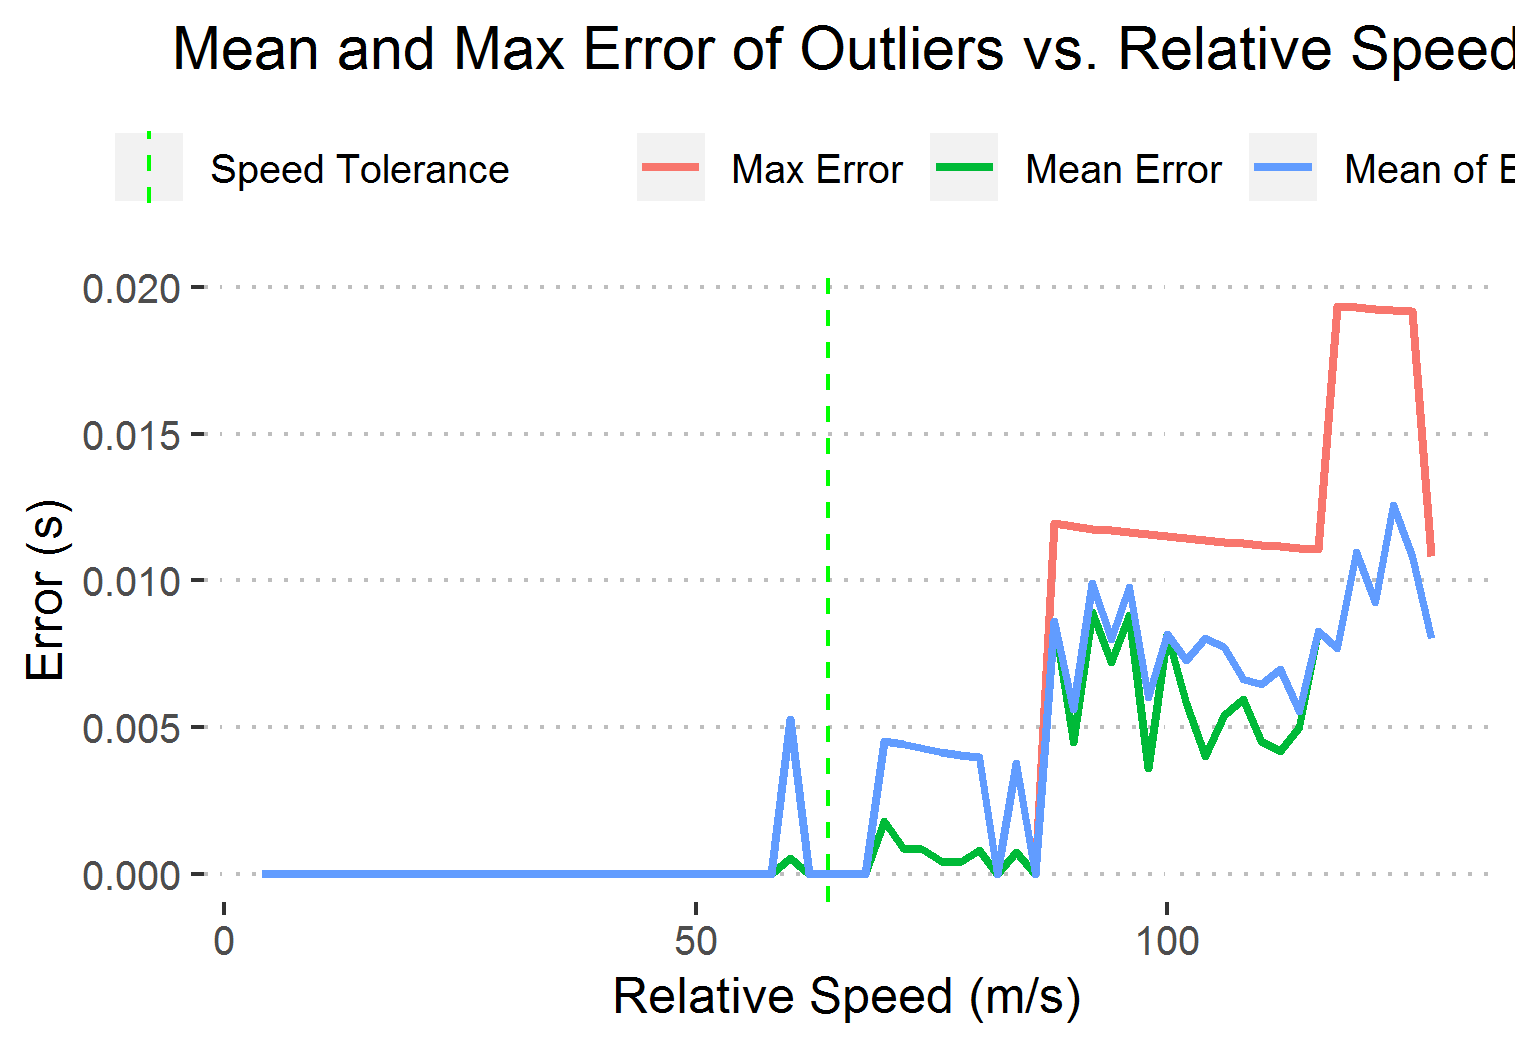
\includegraphics[width=\textwidth]{MeanMaxErrorVsSpeed}
%\caption{The mean and max of collision errors with varying relative speed}
%\label{fig_MeanMaxErrorVsSpeed}
%\end{figure}
%
%\begin{figure}
%\centering
%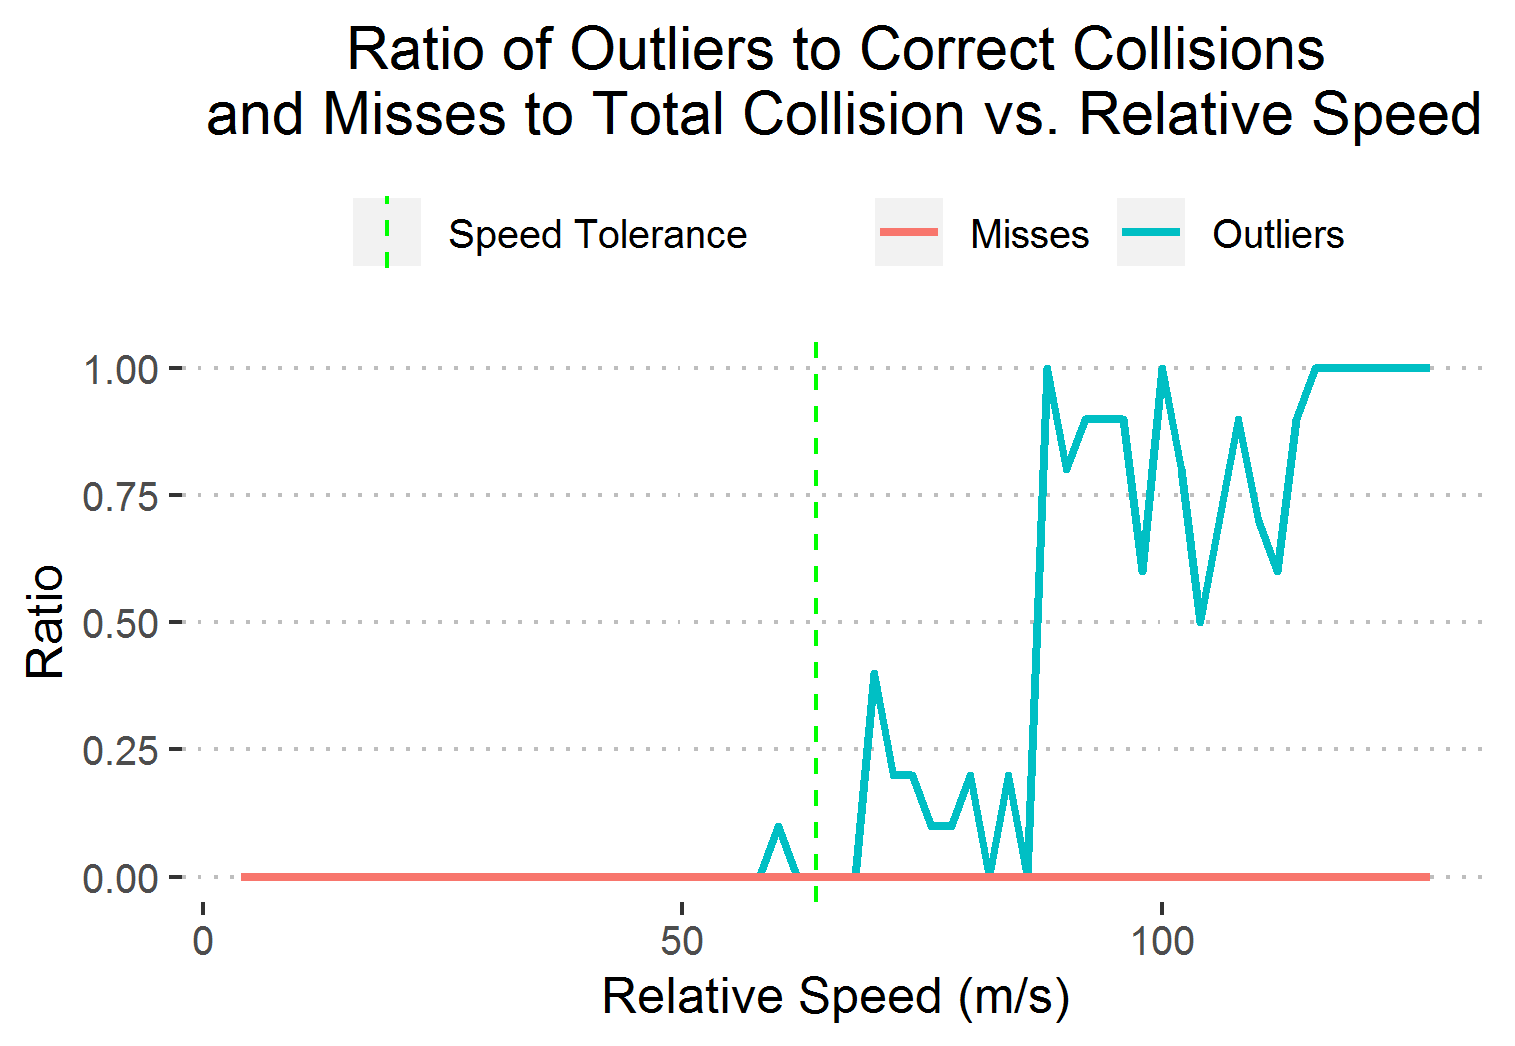
\includegraphics[width=\textwidth]{RatiosVsSpeed}
%\caption{The ratios of erroneous collisions to correct collisions and missed collisions to total collisions with varying relative speed}
%\label{fig_RatiosVsSpeed}
%\end{figure}

The second experiment conducted was the varying latency experiment. In this experiment the latency between the two servers was varied from $0ms$ to double the following tolerances: $2ms$; $8ms$ and $16ms$ in increments of $0.05ms$, $0.25ms$ and $1ms$ respectively. The latency used is the target latency, in reality the latency will never exactly be equal to $0ms$.

\begin{figure}
	\centering
	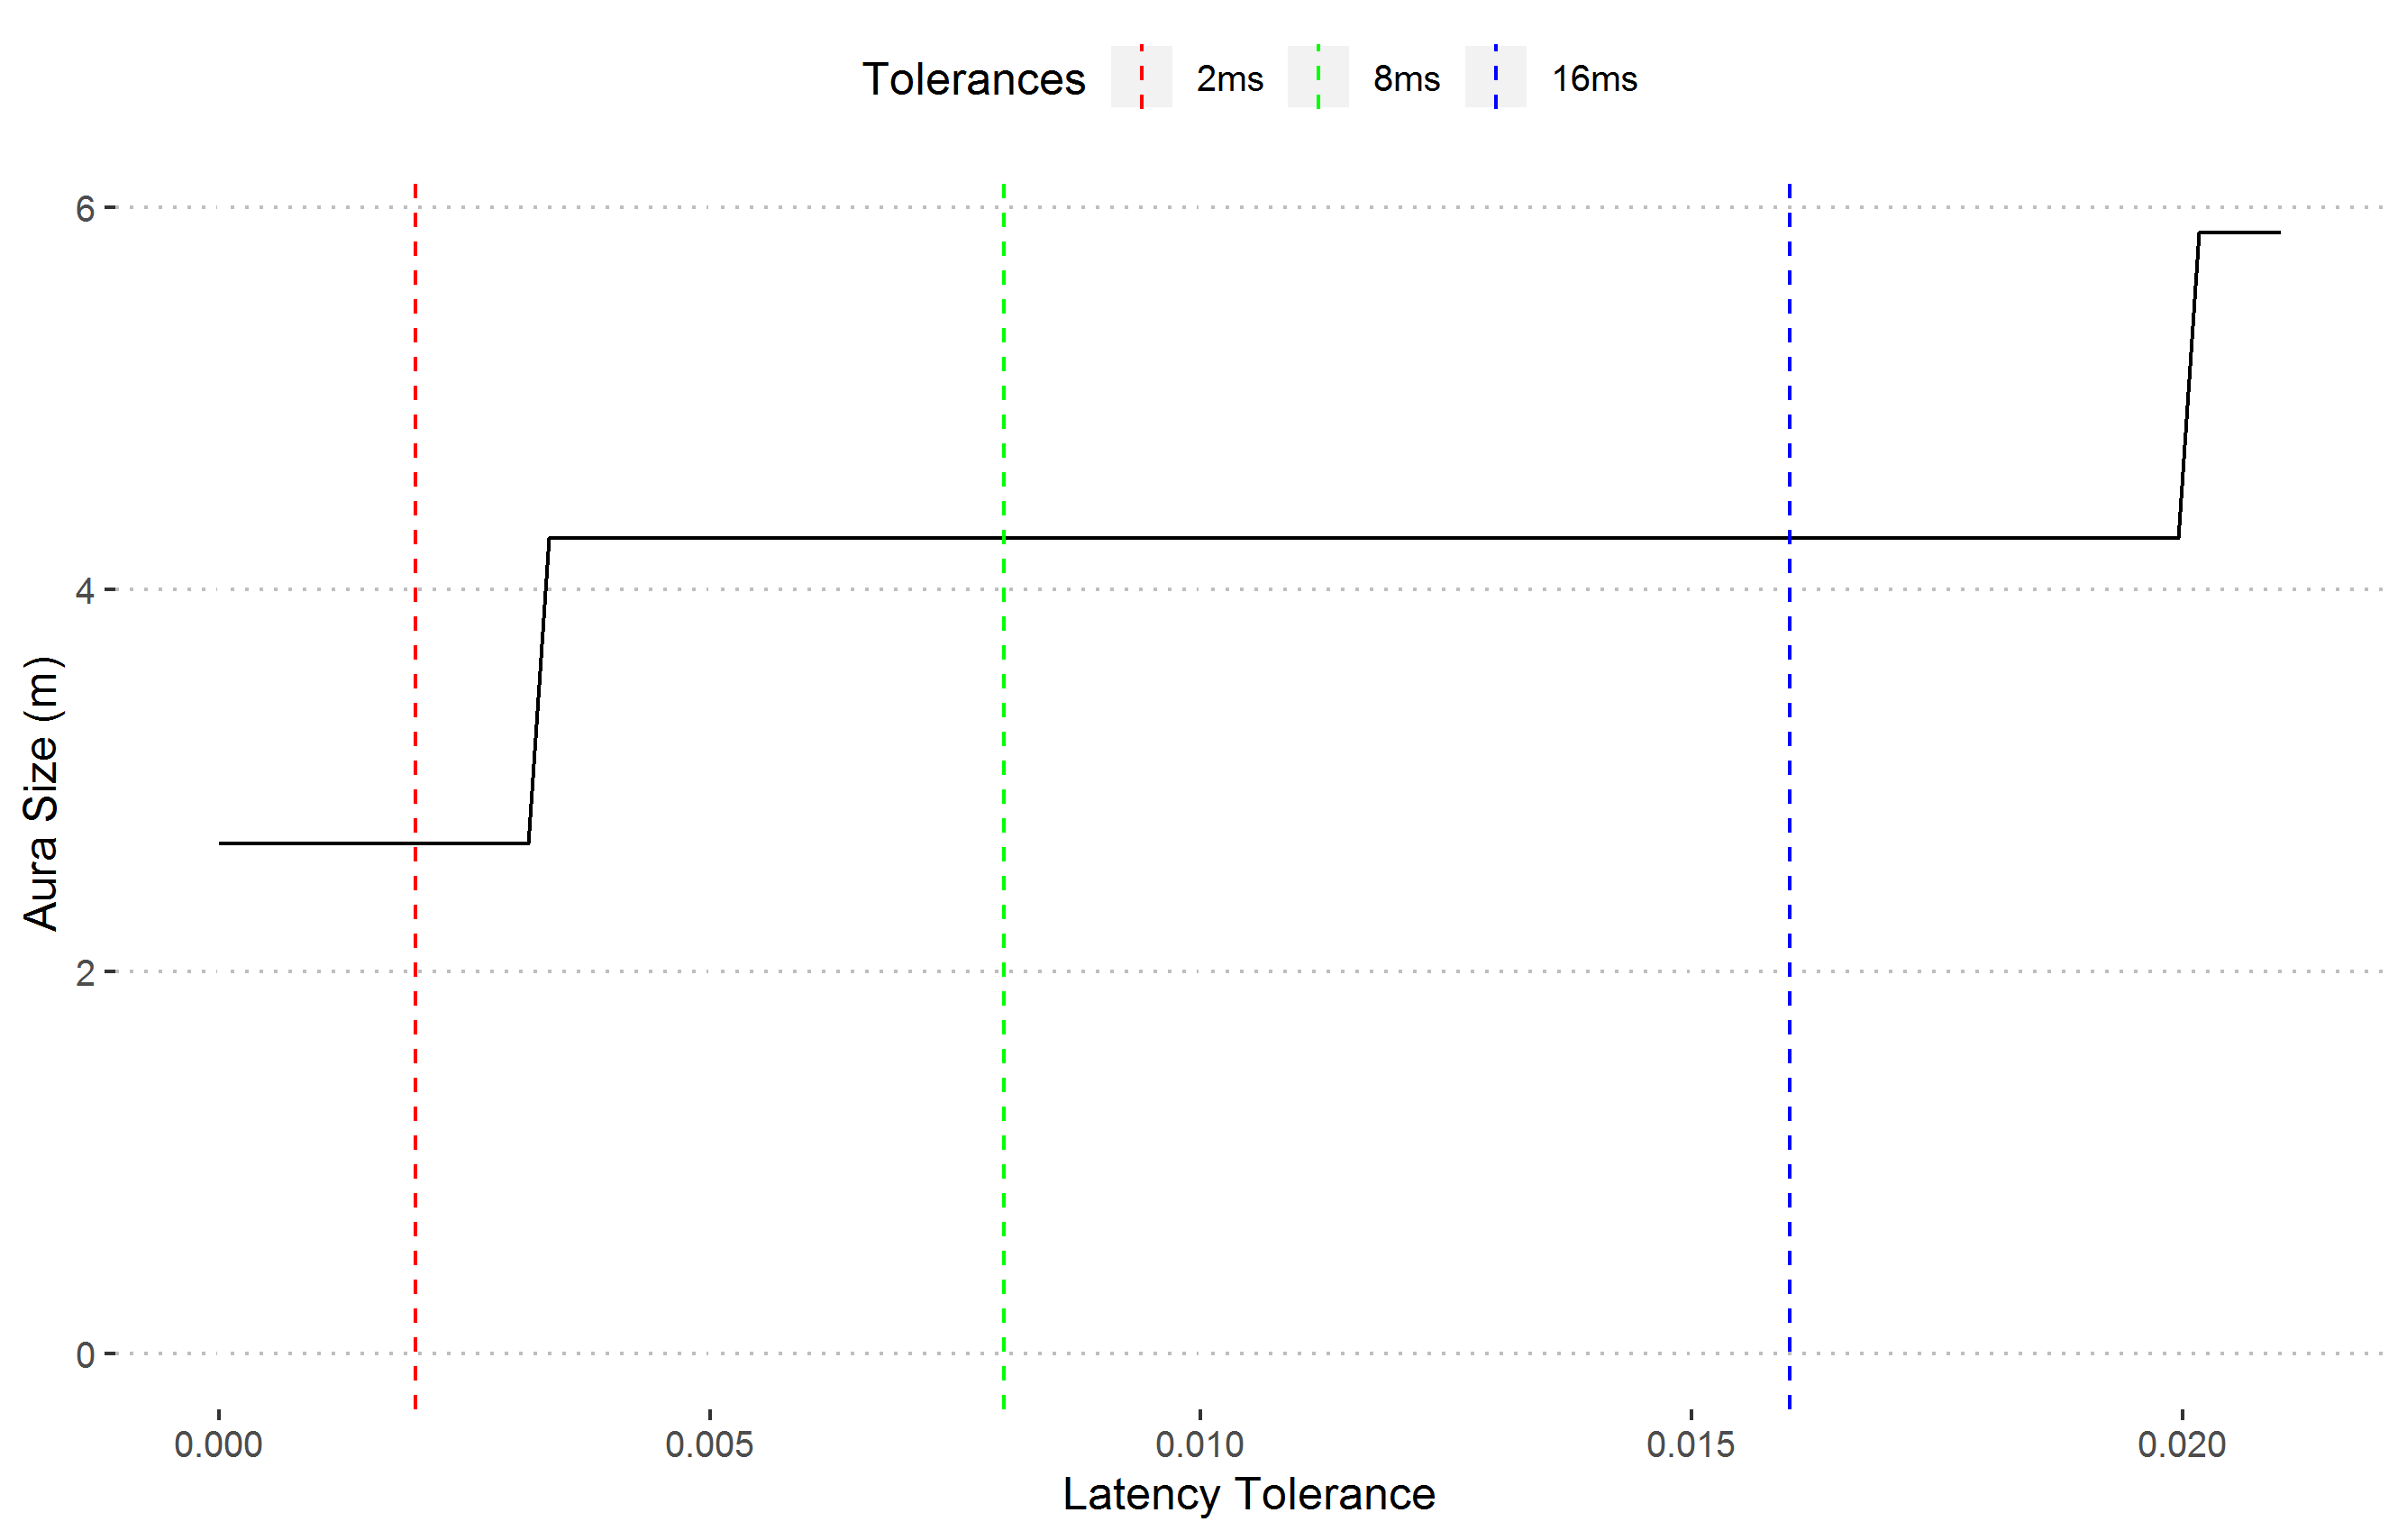
\includegraphics[width=\textwidth]{LatencyAuraSizes}
	\caption{Size of aura vs. latency tolerance. The latency tolerances used are marked in dashed lines}
	\label{fig_LatencyAuraSize}
\end{figure}

Fig. \ref{fig_LatencyAuraSize} shows the size of the aura (not including the bounding sphere of the object) vs increasing latency tolerance, calculated using equation \ref{auraEquation}. The aura size increases discretely with latency tolerance, for example tolerance values from $4ms$ to $20ms$ result in the same aura size. Late collisions are expected to occur only once the actual latency exceeds the maximum tolerance for the current aura size. In the following experiments, this means that in the $2ms$ tolerance experiments, late collisions are not expected to occur until the actual latency exceeds $3ms$. Likewise, in the $8ms$ and $16ms$ tolerance experiments, $20ms$ actual latency is expected to be reached before late collisions begin to occur. Note that late collisions are not expected for the $8ms$ experiment, as $20ms$ latency is not reached. False-positives are expected due to the frame-time delay method and should increase as actual latency increases.

\begin{figure}
	\centering
	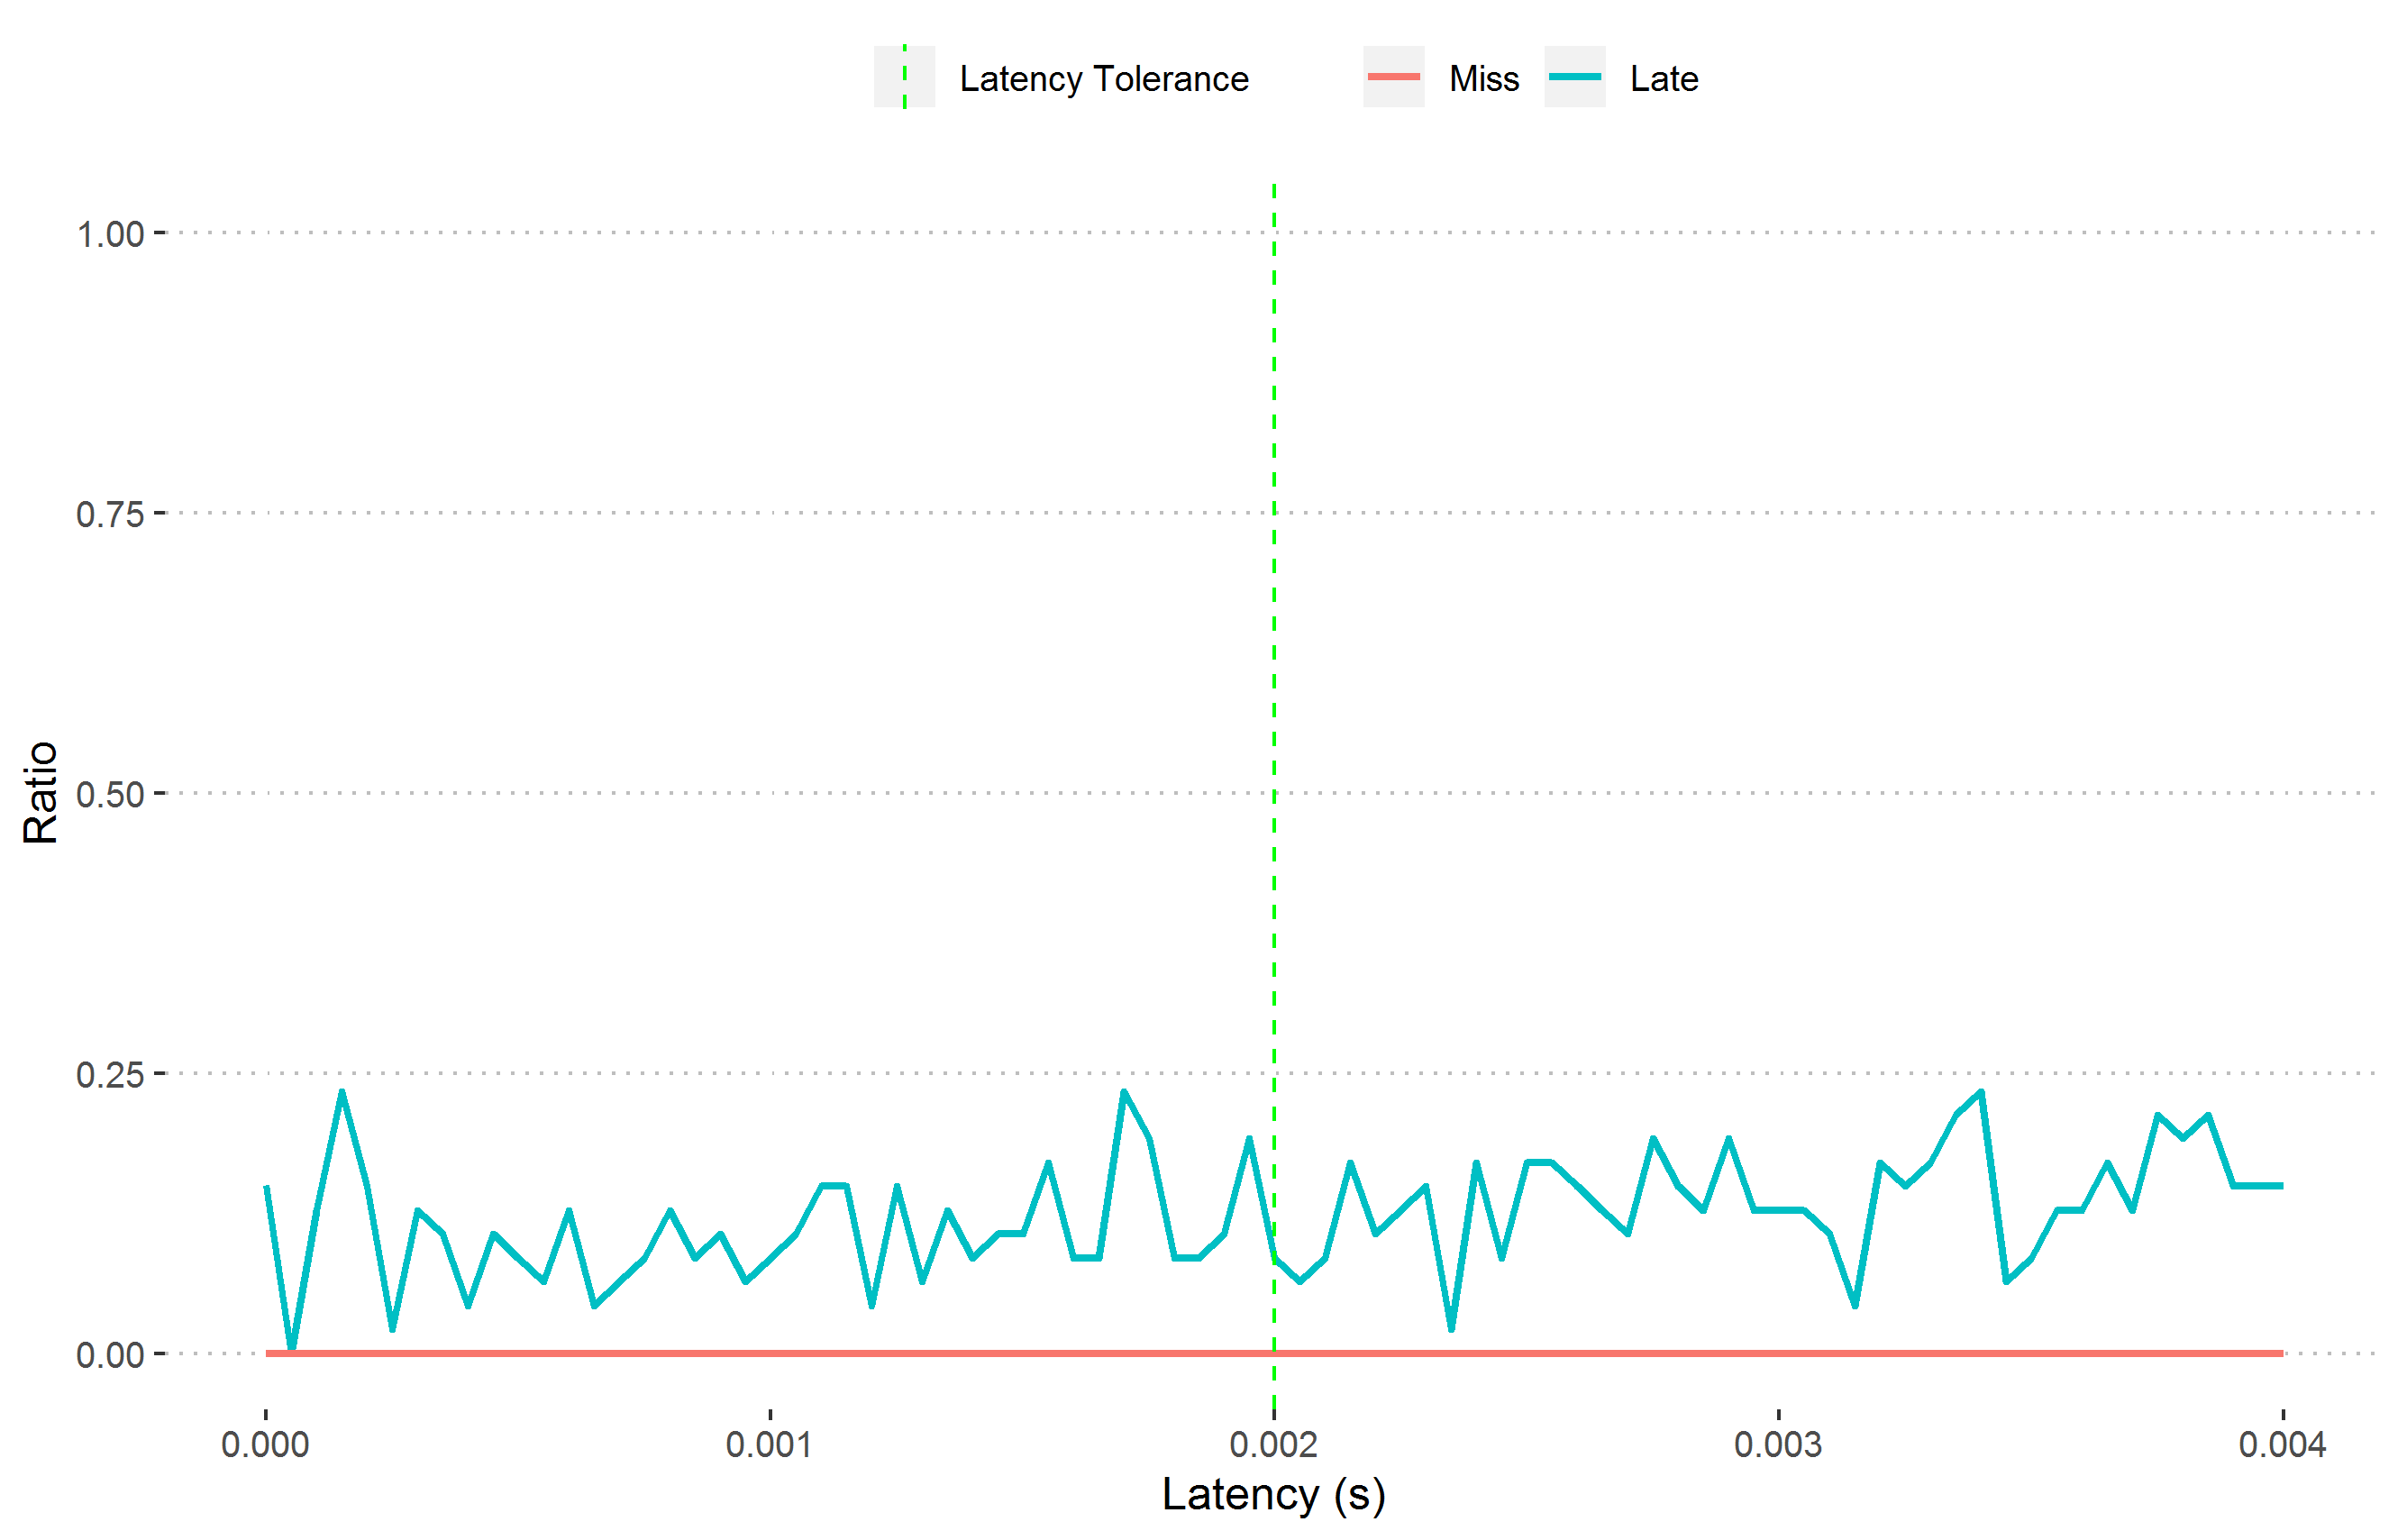
\includegraphics[width=\textwidth]{RatiosVsLatencyLow}
	\caption{Ratio of Late to Correct Collisions and Misses to Total Collision vs. Latency using a latency tolerance of $2ms$. The latency tolerance is marked in a dashed green line.}
	\label{fig_RatioVsLatencyLow}
\end{figure}
\begin{figure}
	\centering
	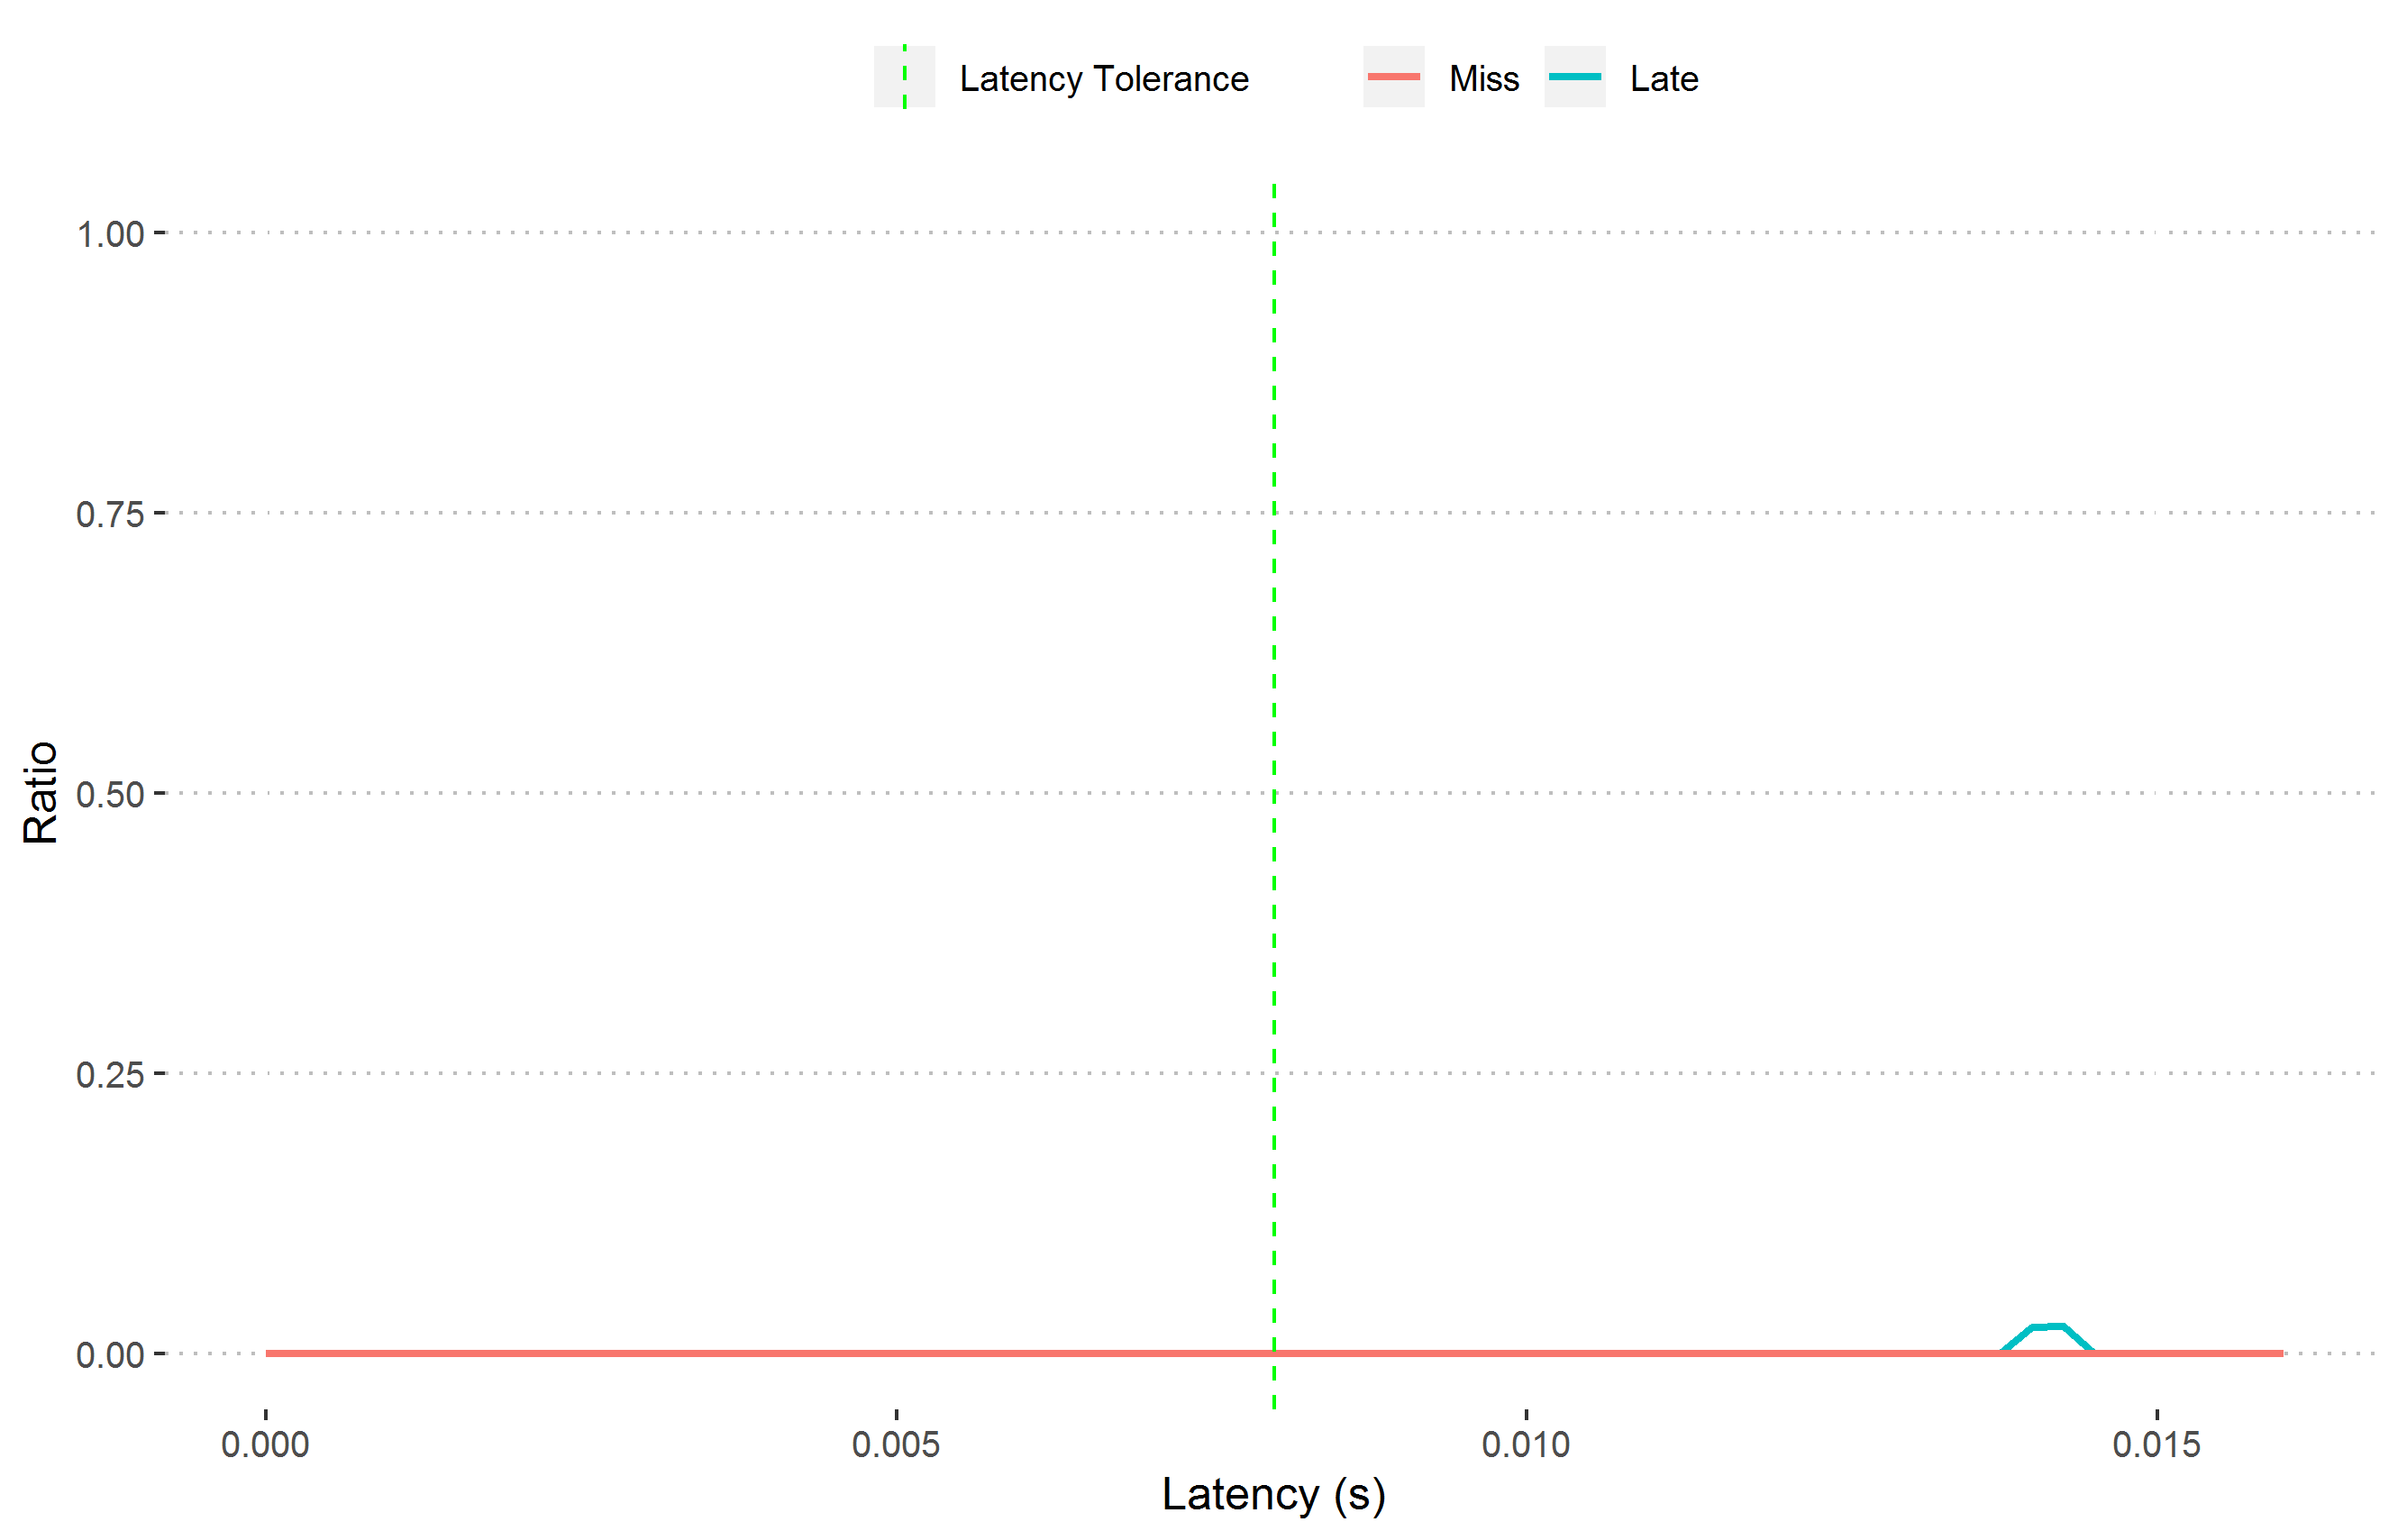
\includegraphics[width=\textwidth]{RatiosVsLatencyMid}
	\caption{Ratio of Late to Correct Collisions and Misses to Total Collision vs. Latency using a latency tolerance of $8ms$. The latency tolerance is marked in a dashed green line.}
	\label{fig_RatioVsLatencyMid}
\end{figure}
\begin{figure}
	\centering
	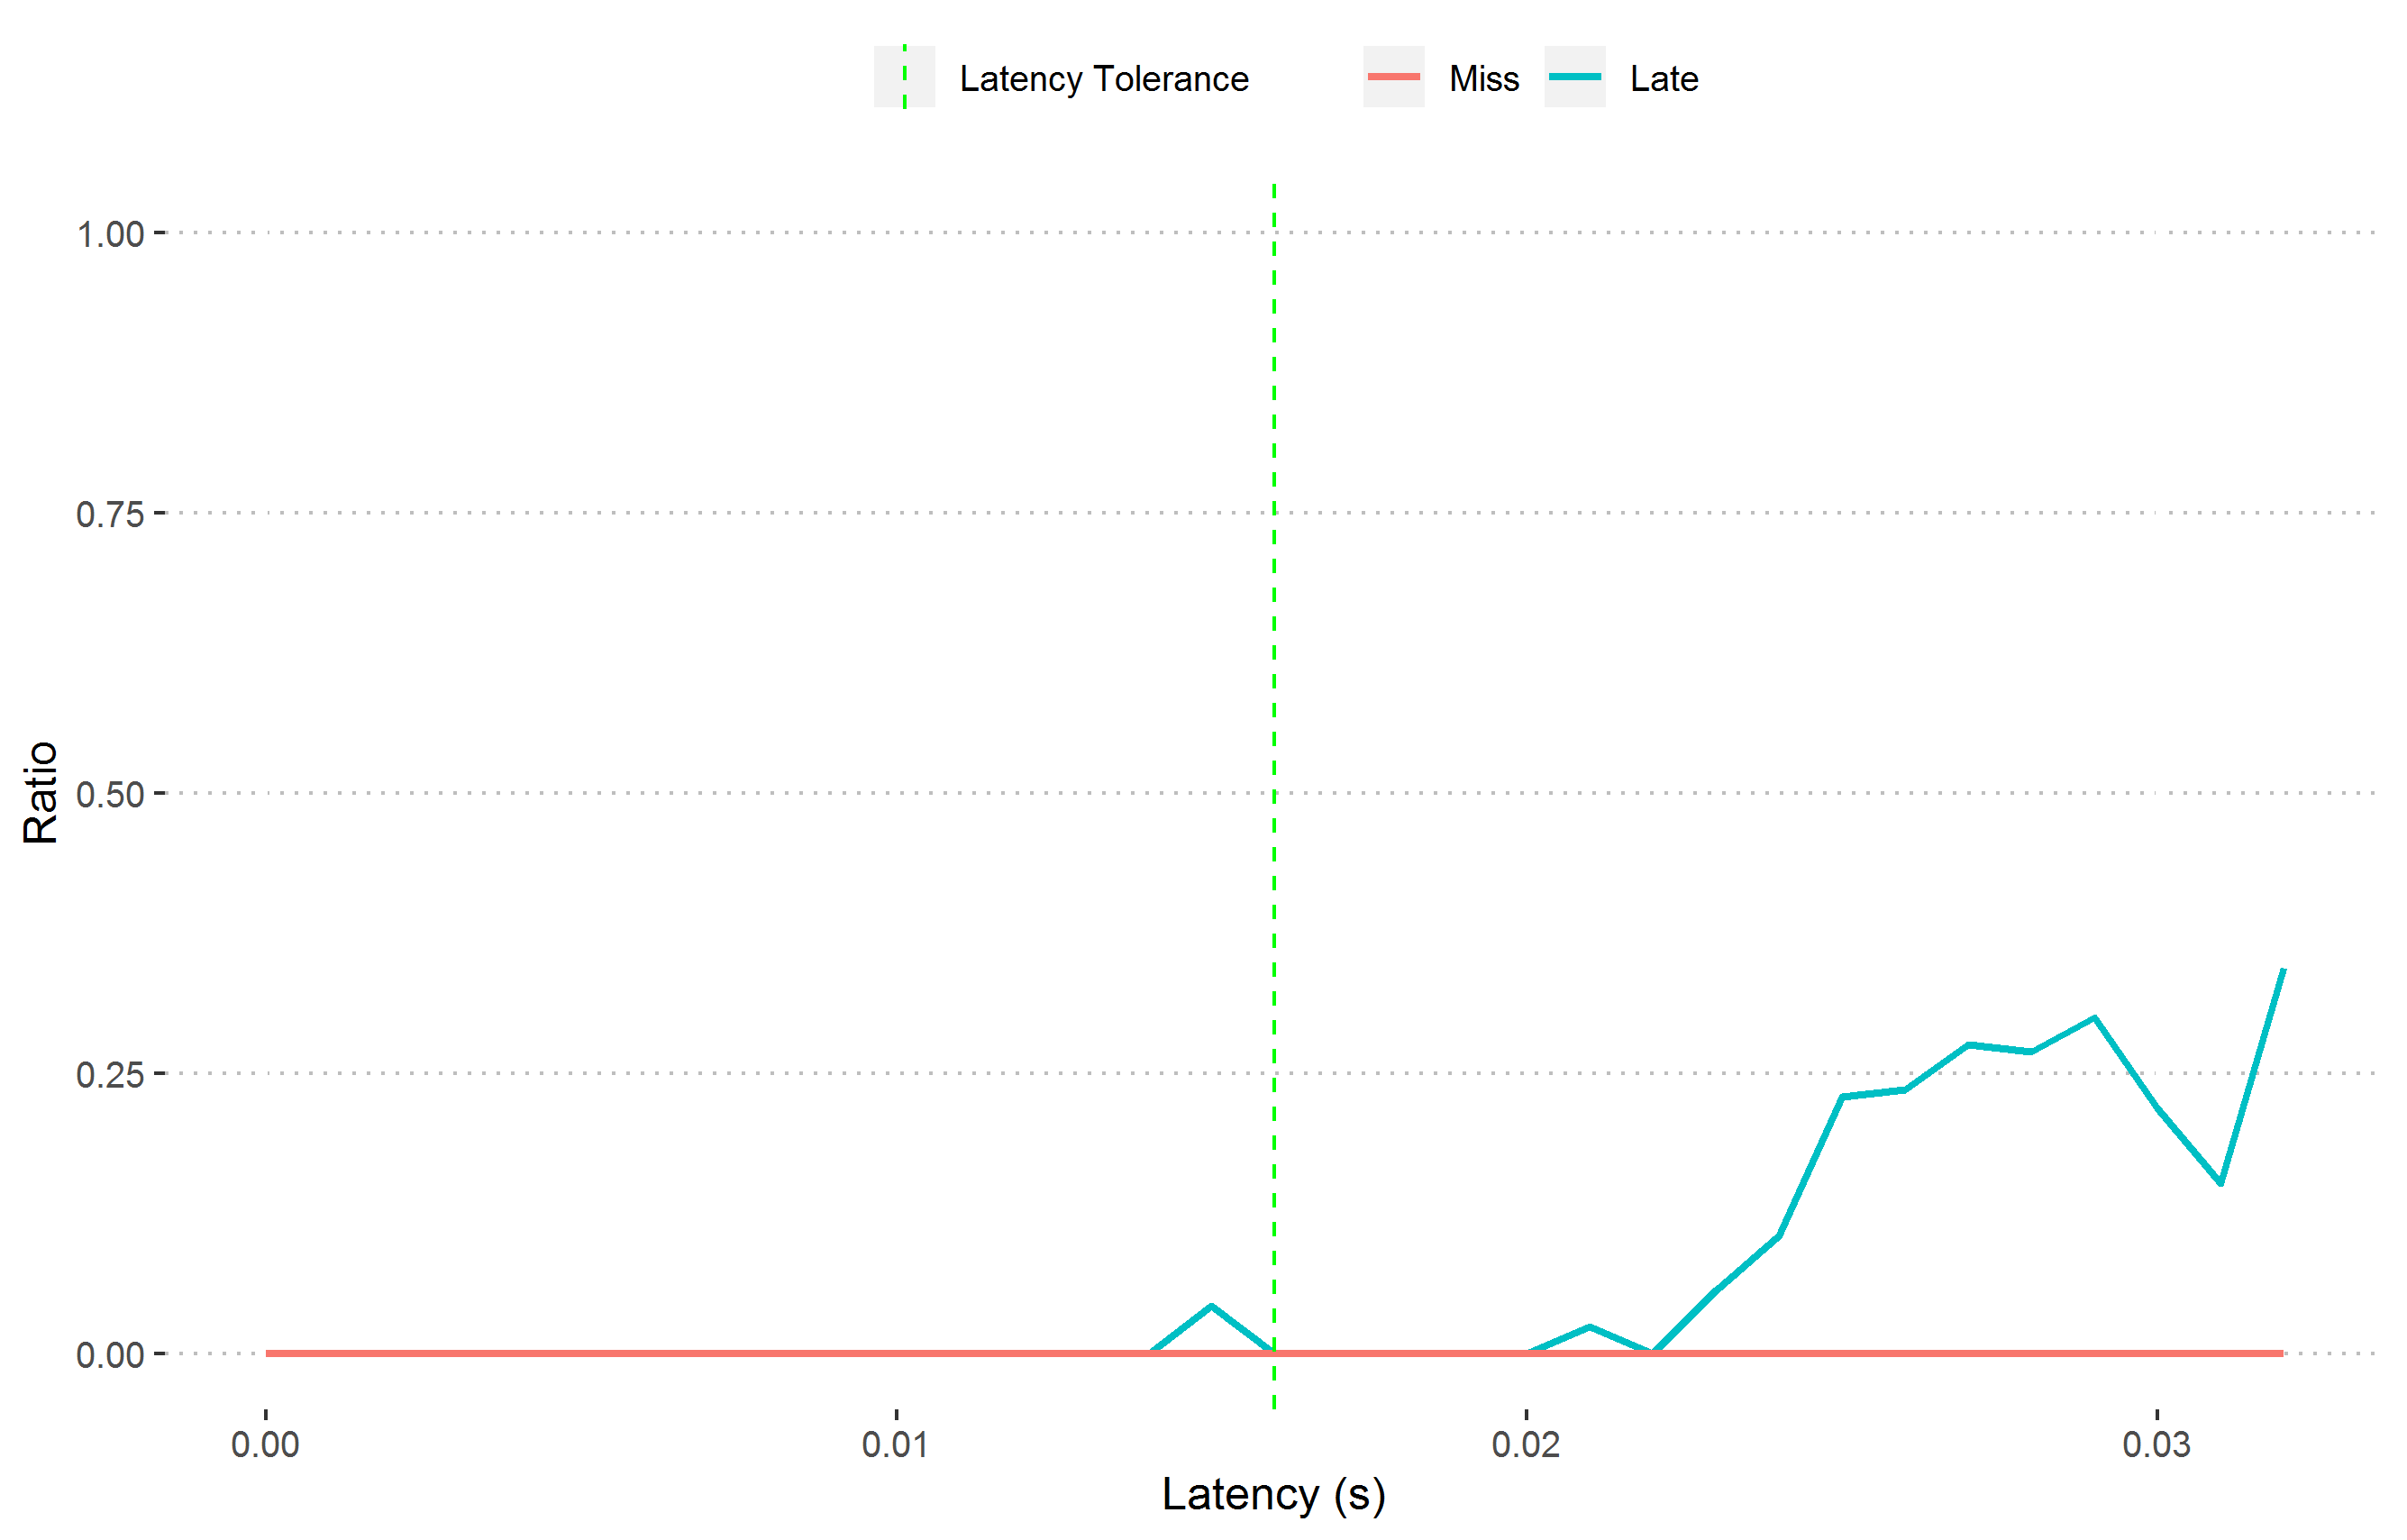
\includegraphics[width=\textwidth]{RatiosVsLatencyHigh}
	\caption{Ratio of Late to Correct Collisions and Misses to Total Collision vs. Latency using a latency tolerance of $16ms$. The latency tolerance is marked in a dashed green line.}
	\label{fig_RatioVsLatencyHigh}
\end{figure}

\begin{figure}
	\centering
	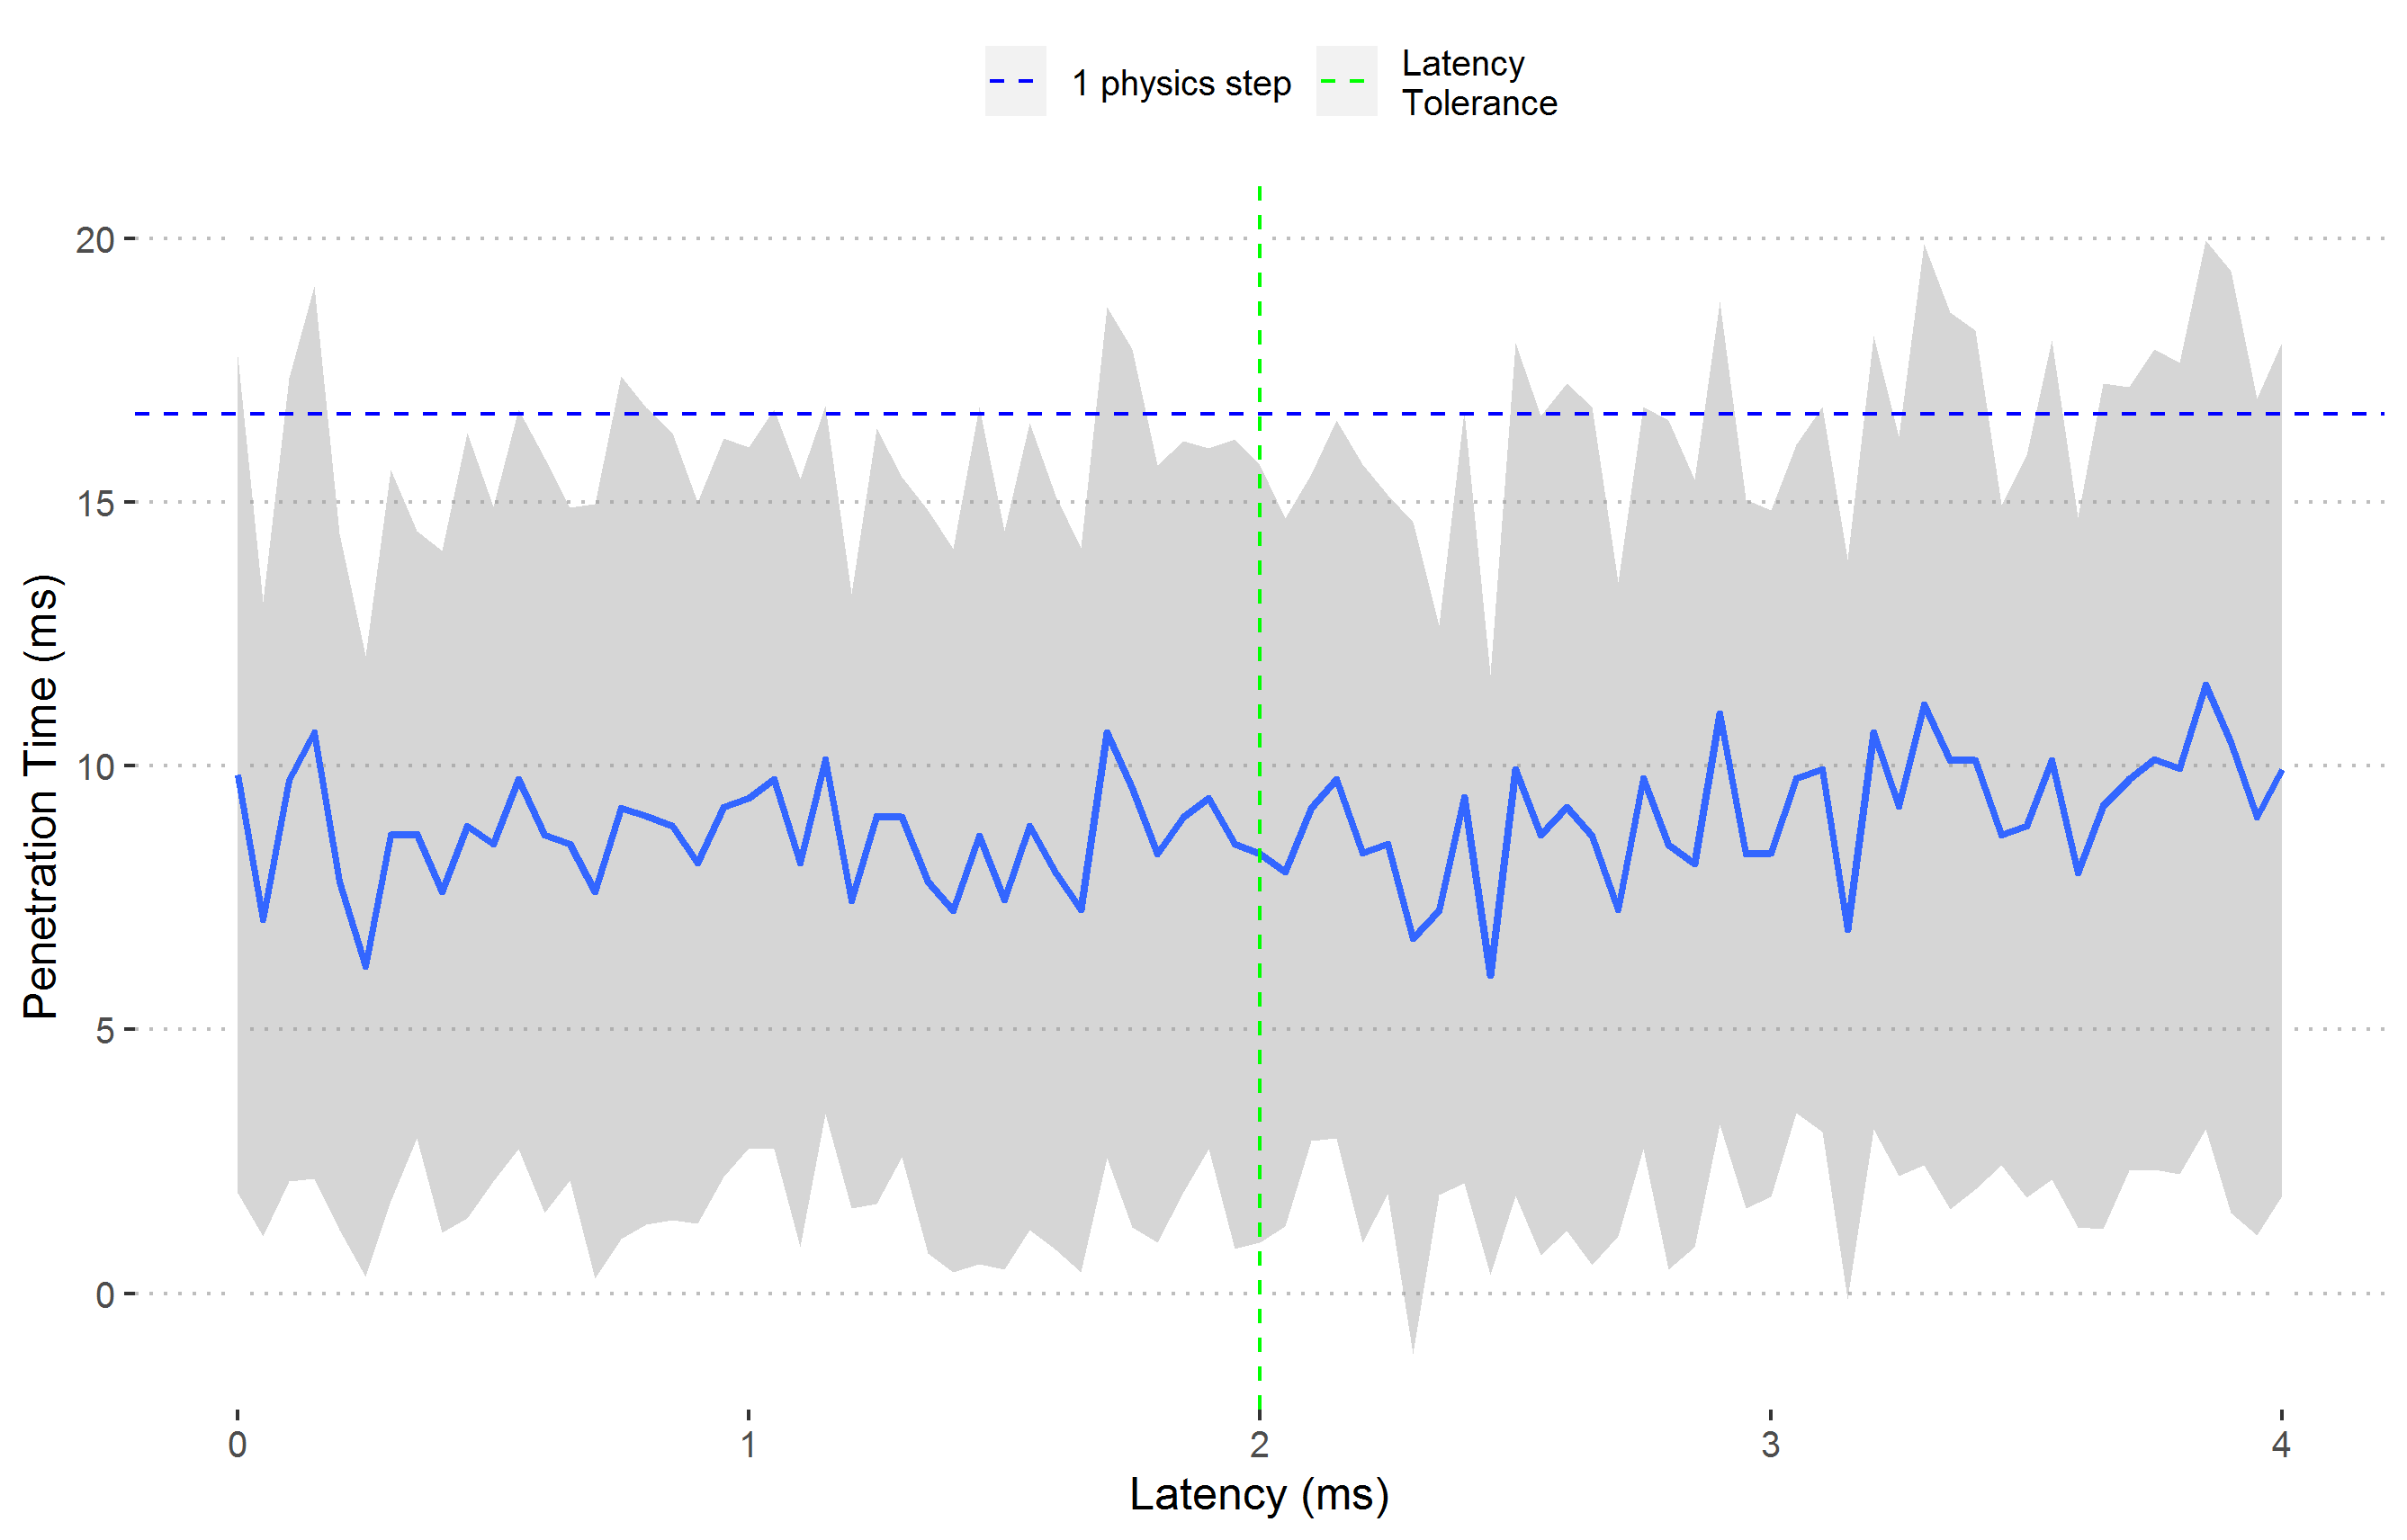
\includegraphics[width=\textwidth]{MeanPenVsLatencyLow}
	\caption{Mean penetration time of objects with $+/-2$ standard deviations with varying latency using a latency tolerance of $2ms$. The maximum expected penetration time of 1 physics step is marked with a dashed blue line. The latency tolerance is marked in a dashed green line.}
	\label{fig_CollisionsPenVsLatencyLow}
\end{figure}
\begin{figure}
	\centering
	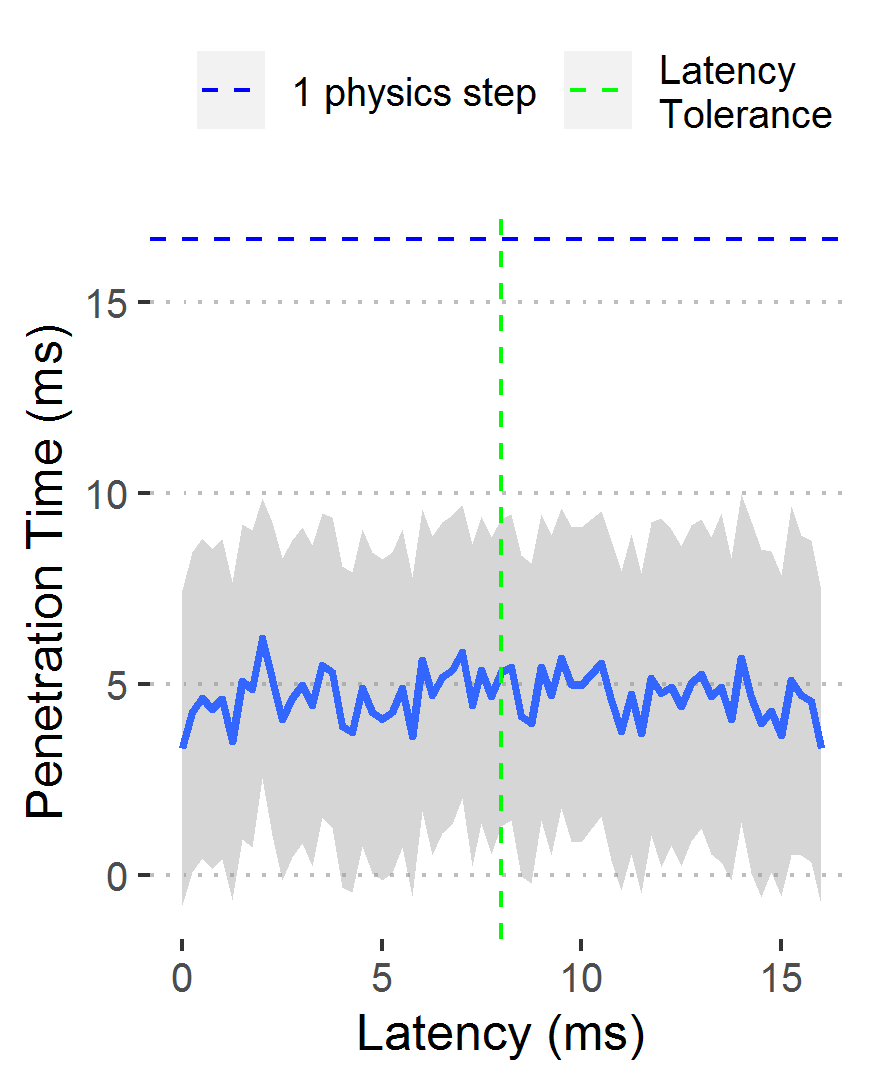
\includegraphics[width=\textwidth]{MeanPenVsLatencyMid}
	\caption{Mean penetration time of objects with $+/-2$ standard deviations with varying latency using a latency tolerance of $8ms$. The maximum expected penetration time of 1 physics step is marked with a dashed blue line. The latency tolerance is marked in a dashed green line.}
	\label{fig_CollisionsPenVsLatencyMid}
\end{figure}
\begin{figure}
	\centering
	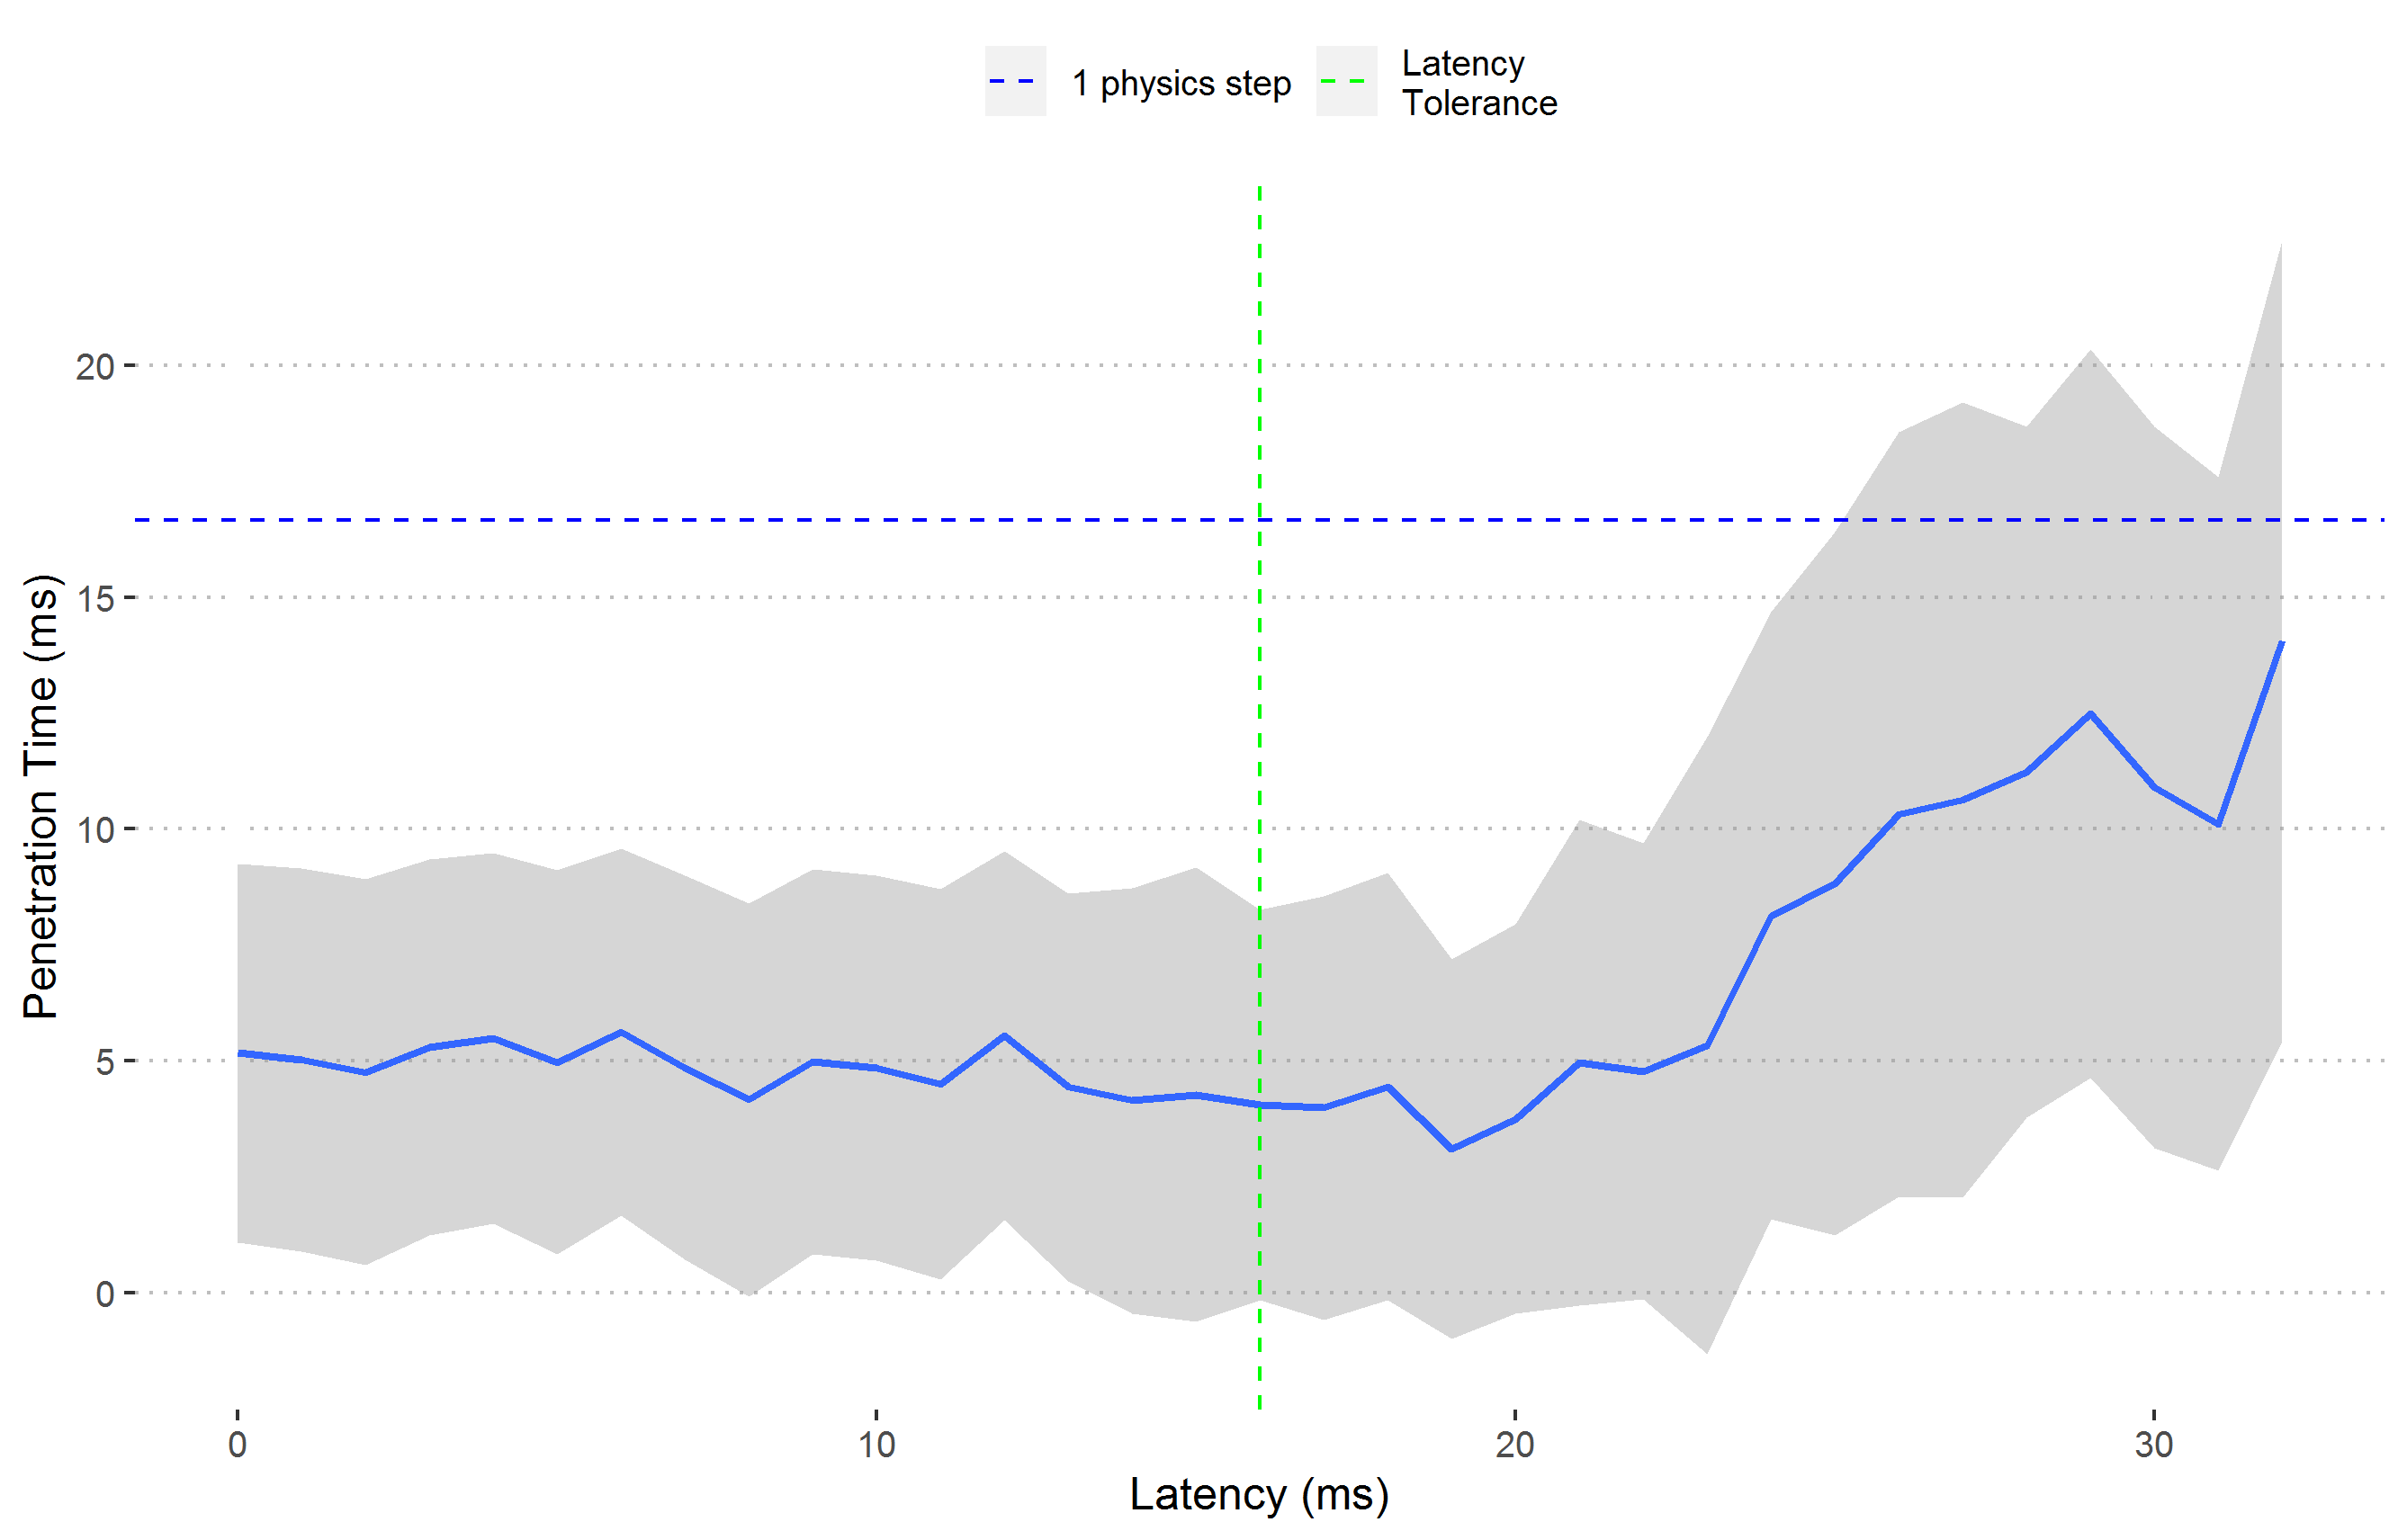
\includegraphics[width=\textwidth]{MeanPenVsLatencyHigh}
	\caption{Mean penetration time of objects with $+/-2$ standard deviations with varying latency using a latency tolerance of $16ms$. The maximum expected penetration time of 1 physics step is marked with a dashed blue line. The latency tolerance is marked in a dashed green line.}
	\label{fig_CollisionsPenVsLatencyHigh}
\end{figure}

%\begin{figure}
%\centering
%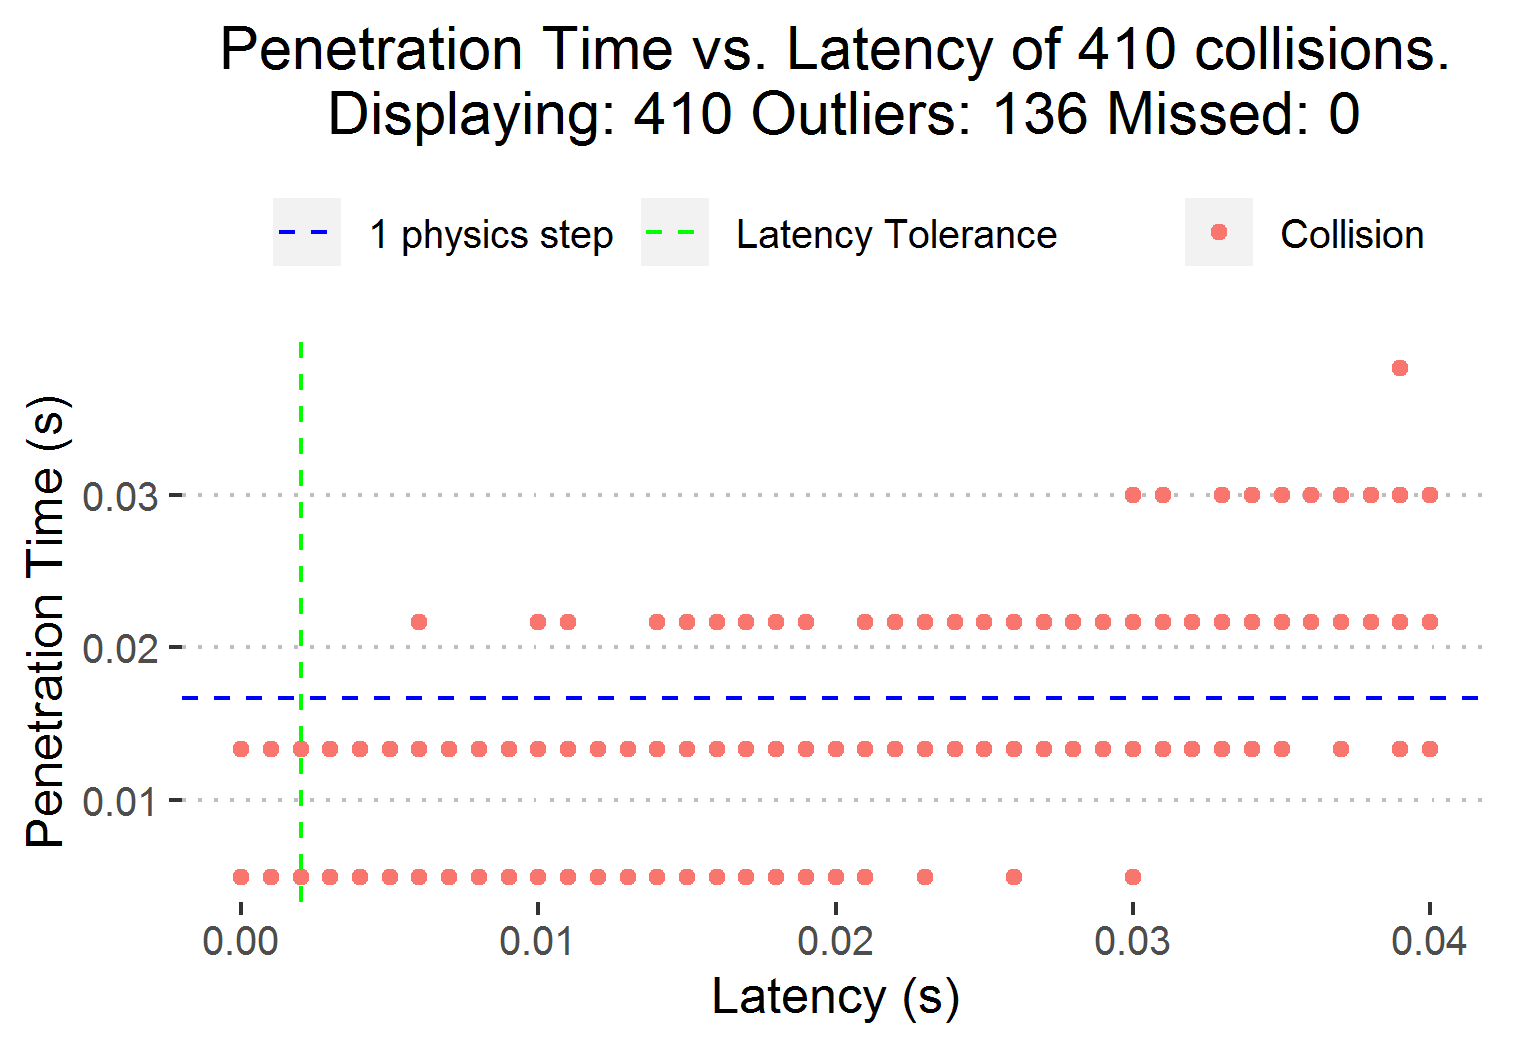
\includegraphics[width=\textwidth]{CollisionsPenVsLatency}
%\caption{Penetration time of objects with varying latency. Each red point represents one or more collisions. The maximum expected penetration time of 1 physics steps is marked with a dashed blue line. The latency tolerance is marked in a dashed green line. The number and magnitude of errors increases as latency increases beyond the tolerance.}
%\label{fig_CollisionsPenVsLatency}
%\end{figure}
%
%\begin{figure}
%\centering
%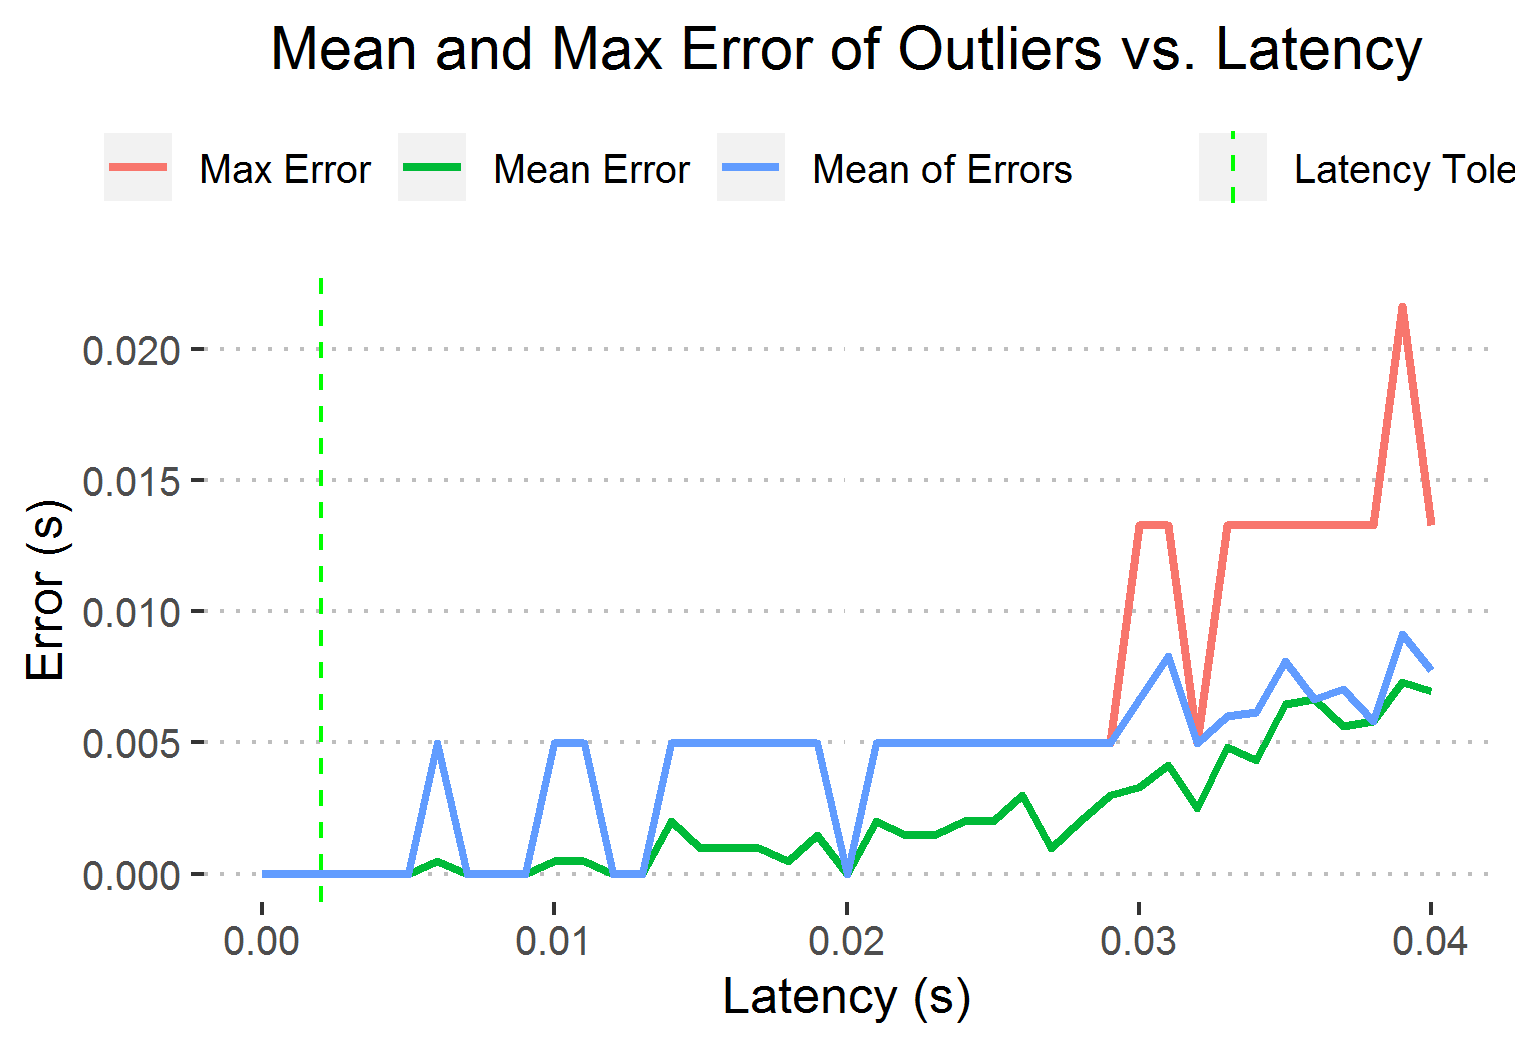
\includegraphics[width=\textwidth]{MeanMaxErrorVsLatency}
%\caption{The mean and max of collision errors with varying latency}
%\label{fig_MeanMaxErrorVsLatency}
%\end{figure}
%
%\begin{figure}
%\centering
%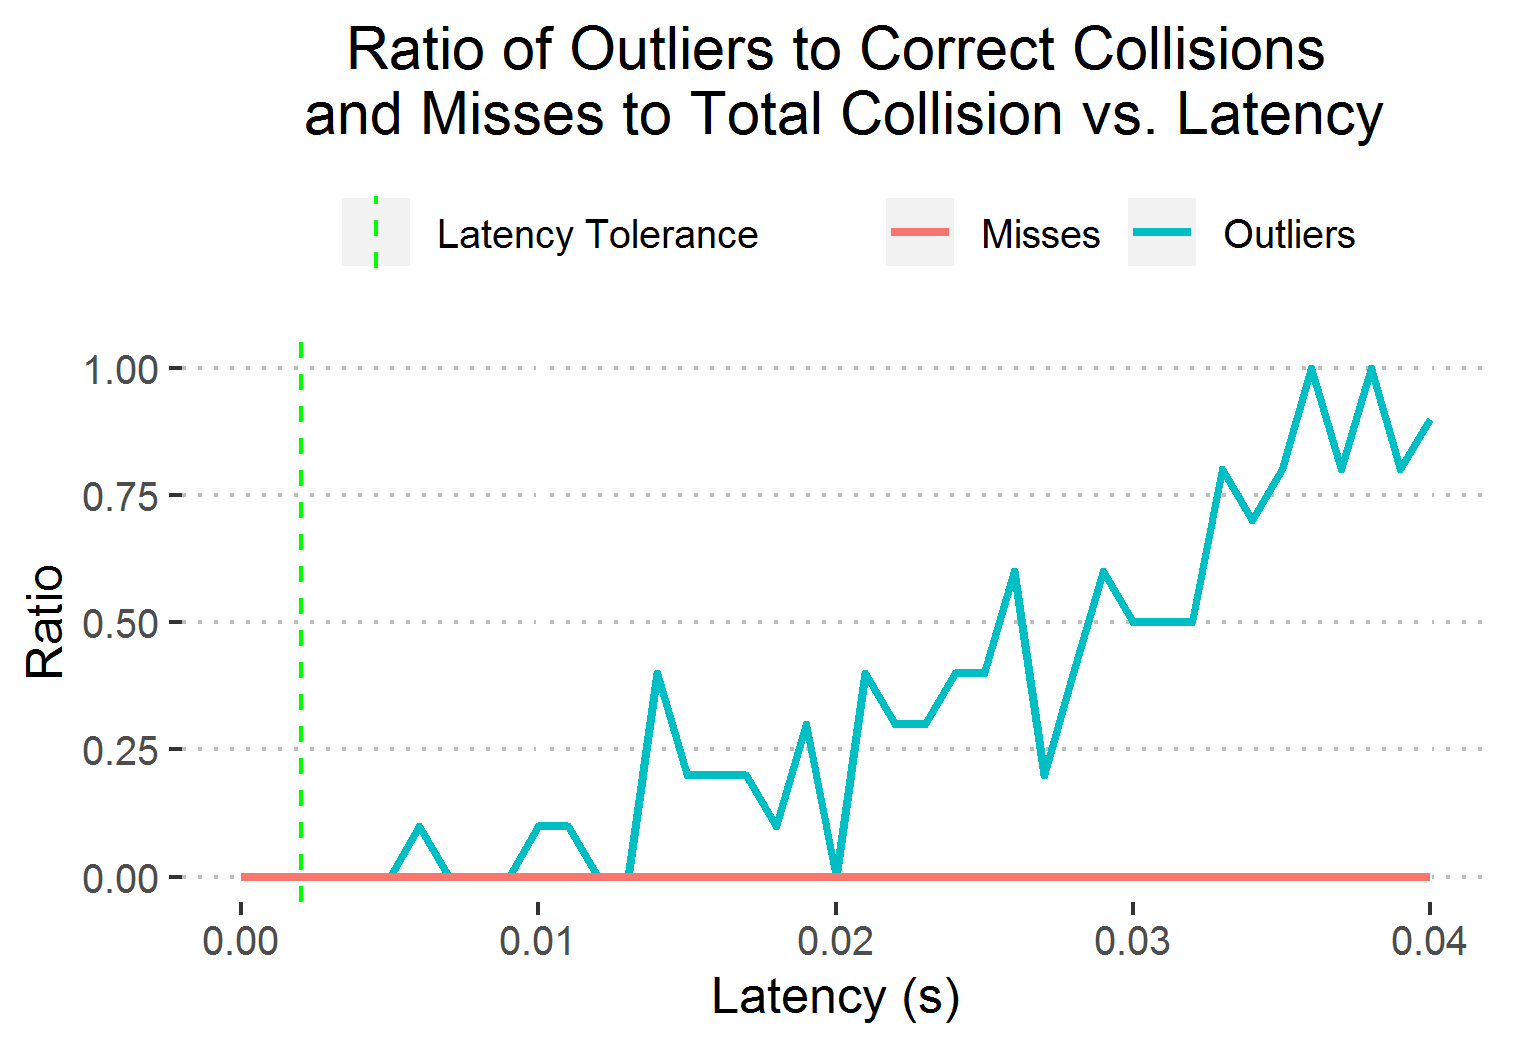
\includegraphics[width=\textwidth]{RatiosVsLatency}
%\caption{The ratios of erroneous collisions to correct collisions and missed collisions to total collisions with varying latency}
%\label{fig_RatiosVsLatency}
%\end{figure}

The third experiment conducted was the varying frame-time experiment. In this experiment the frame-time was varied from $0ms$ to double the frame-time tolerance for the following frame-times: $8.33ms$ $(120Hz)$; $15ms$ $(66.67Hz)$ and $33.33ms$ $(30Hz)$. Increments of $1ms$, $1ms$ and $2ms$ were used respectively. The frame-time used is target frame time, in reality frame-time cannot be equal to exactly $0ms$.

\begin{figure}
	\centering
	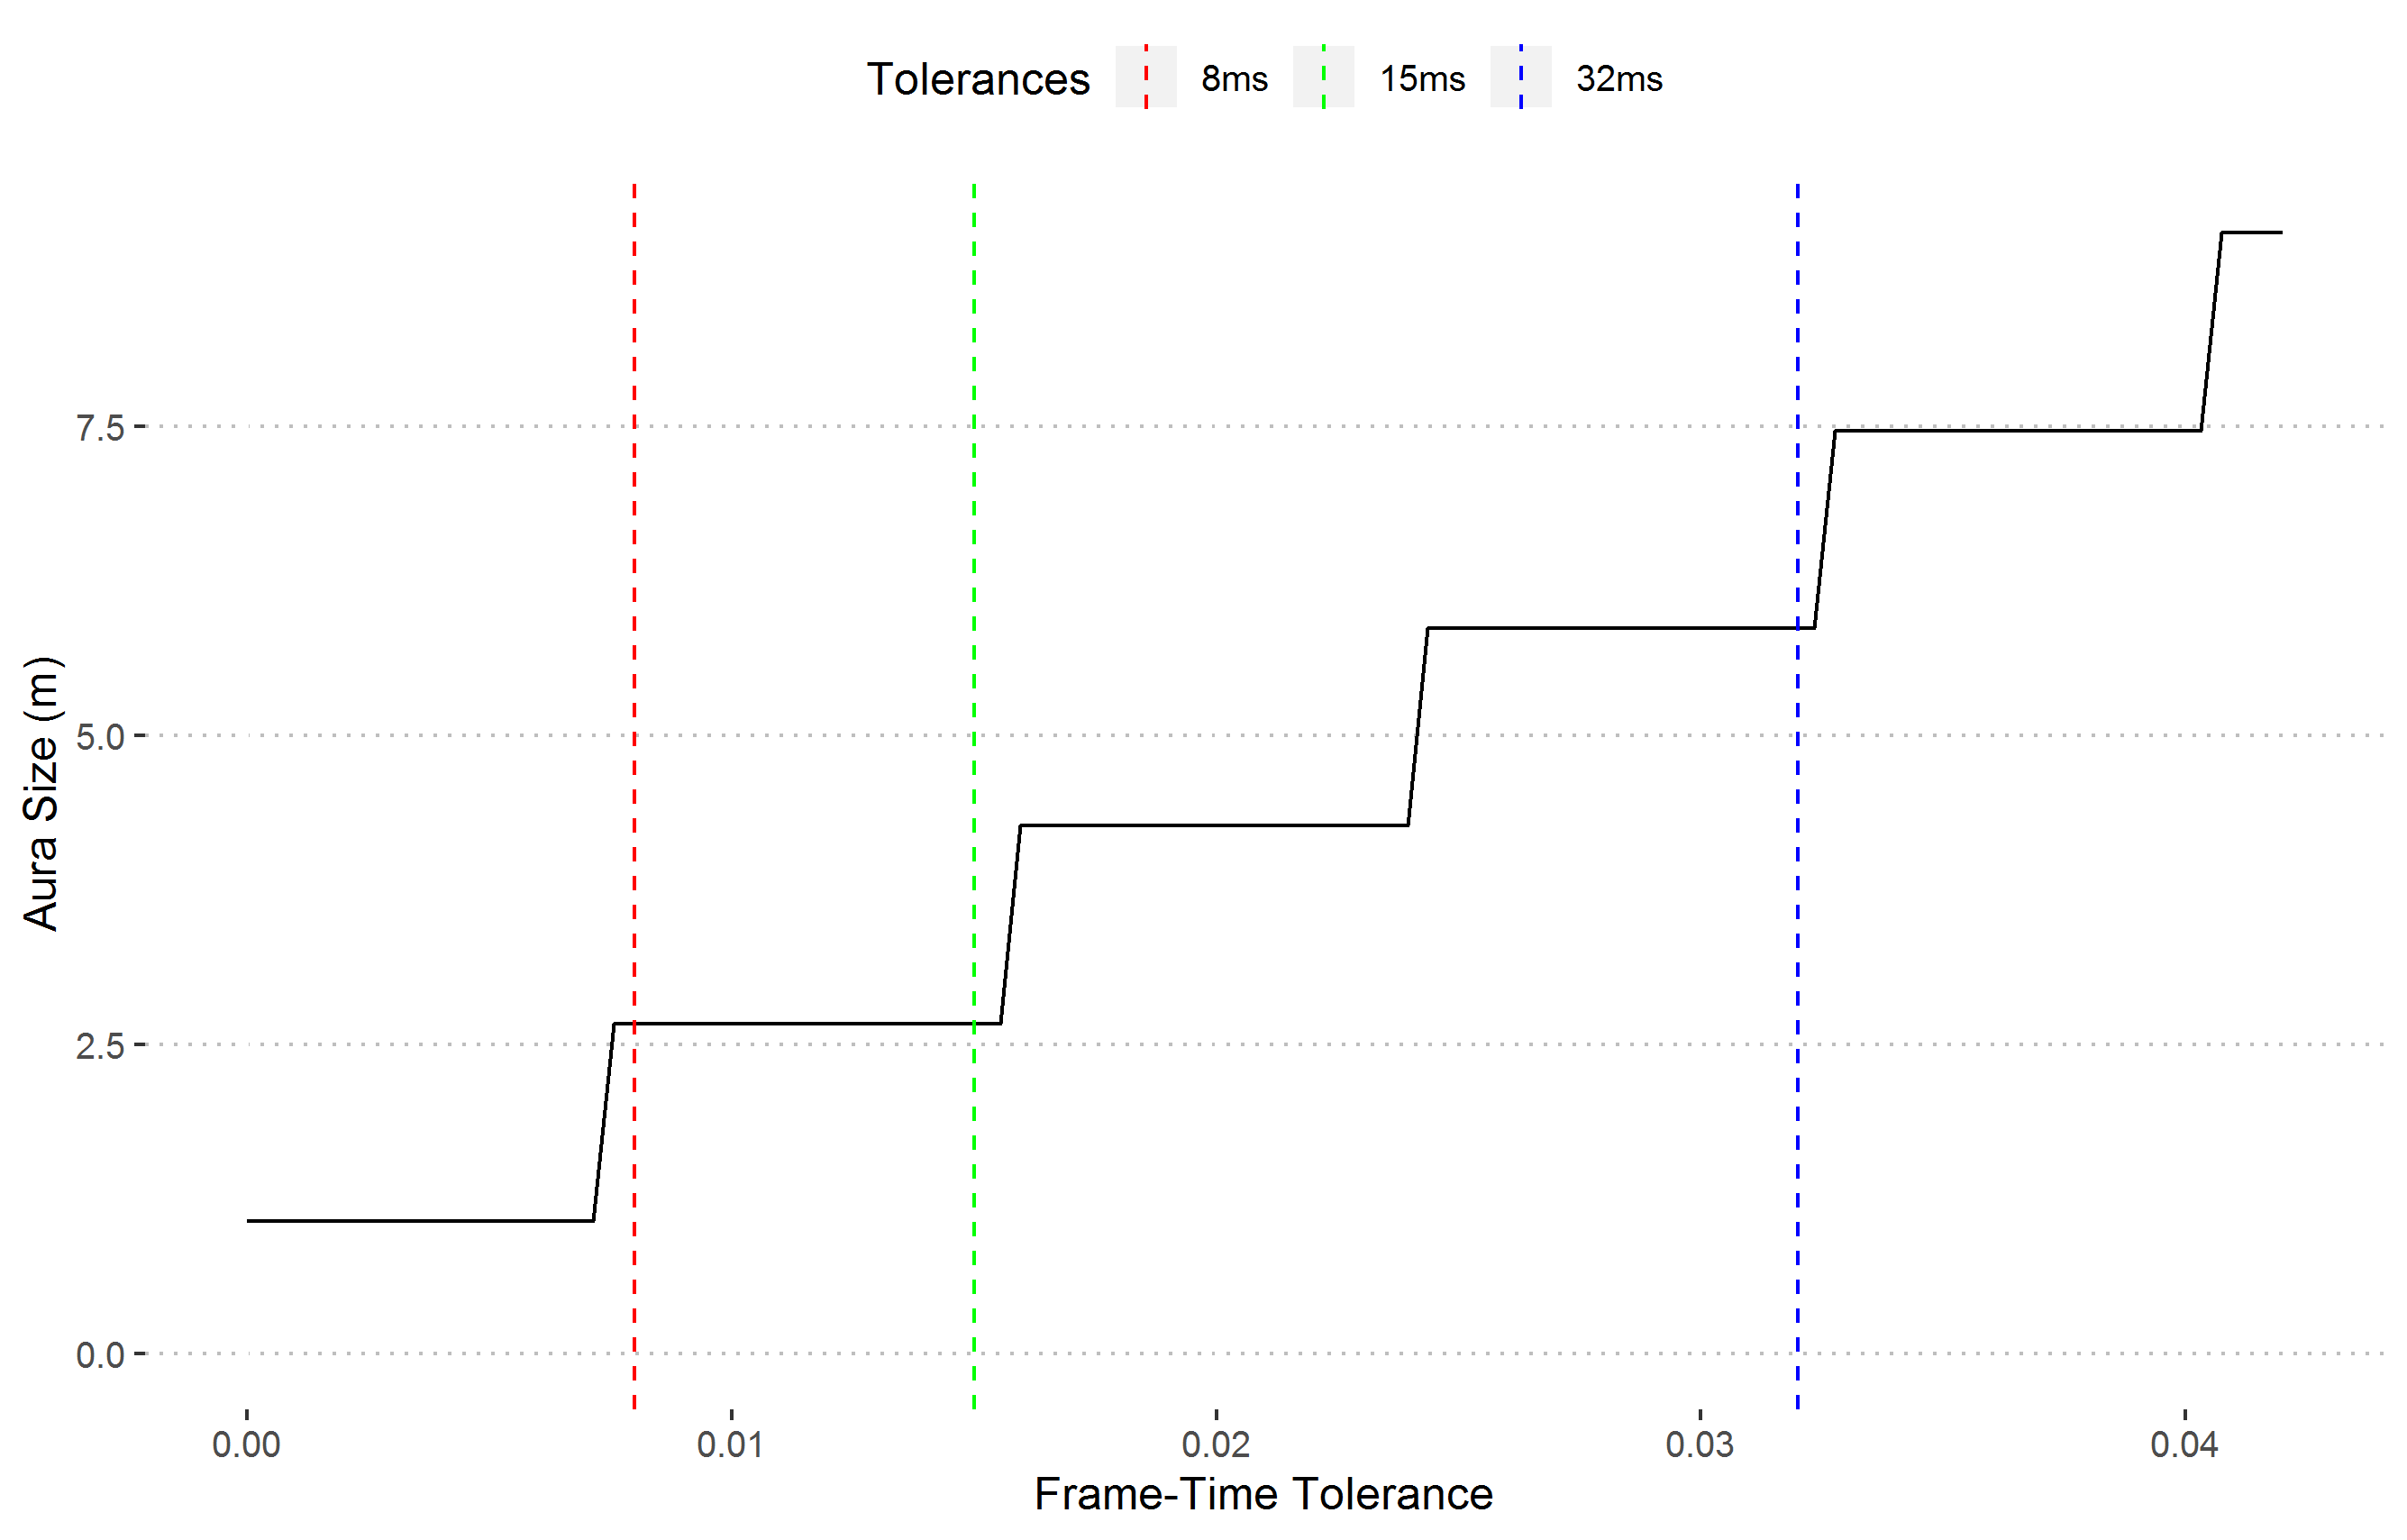
\includegraphics[width=\textwidth]{FrameAuraSizes}
	\caption{Size of aura vs. frame-time tolerance. The frame-time tolerances used are marked in dashed lines}
	\label{fig_FrameTimeAuraSize}
\end{figure}

Fig. \ref{fig_FrameTimeAuraSize} shows the size of the aura (not including the bounding sphere of the object) vs increasing frame-time tolerance, calculated using equation \ref{auraEquation}. The aura size increases discretely with frame-time tolerance, therefore we expect late collisions to begin only once the the actual frame-time is higher than the maximum frame-time the current aura size tolerates. In the varying frame-time experiments, this will be when frame-time reaches $16ms$ for the $8ms$ and $15ms$ tolerance experiments and $32ms$ for the $32ms$ tolerance experiment. Note that late collisions are not expected for the $8ms$ experiment, as $16ms$ frame-time is not exceeded. False-positives are expected due to the frame-time delay method and should increase as frame-time increases.

\begin{figure}
	\centering
	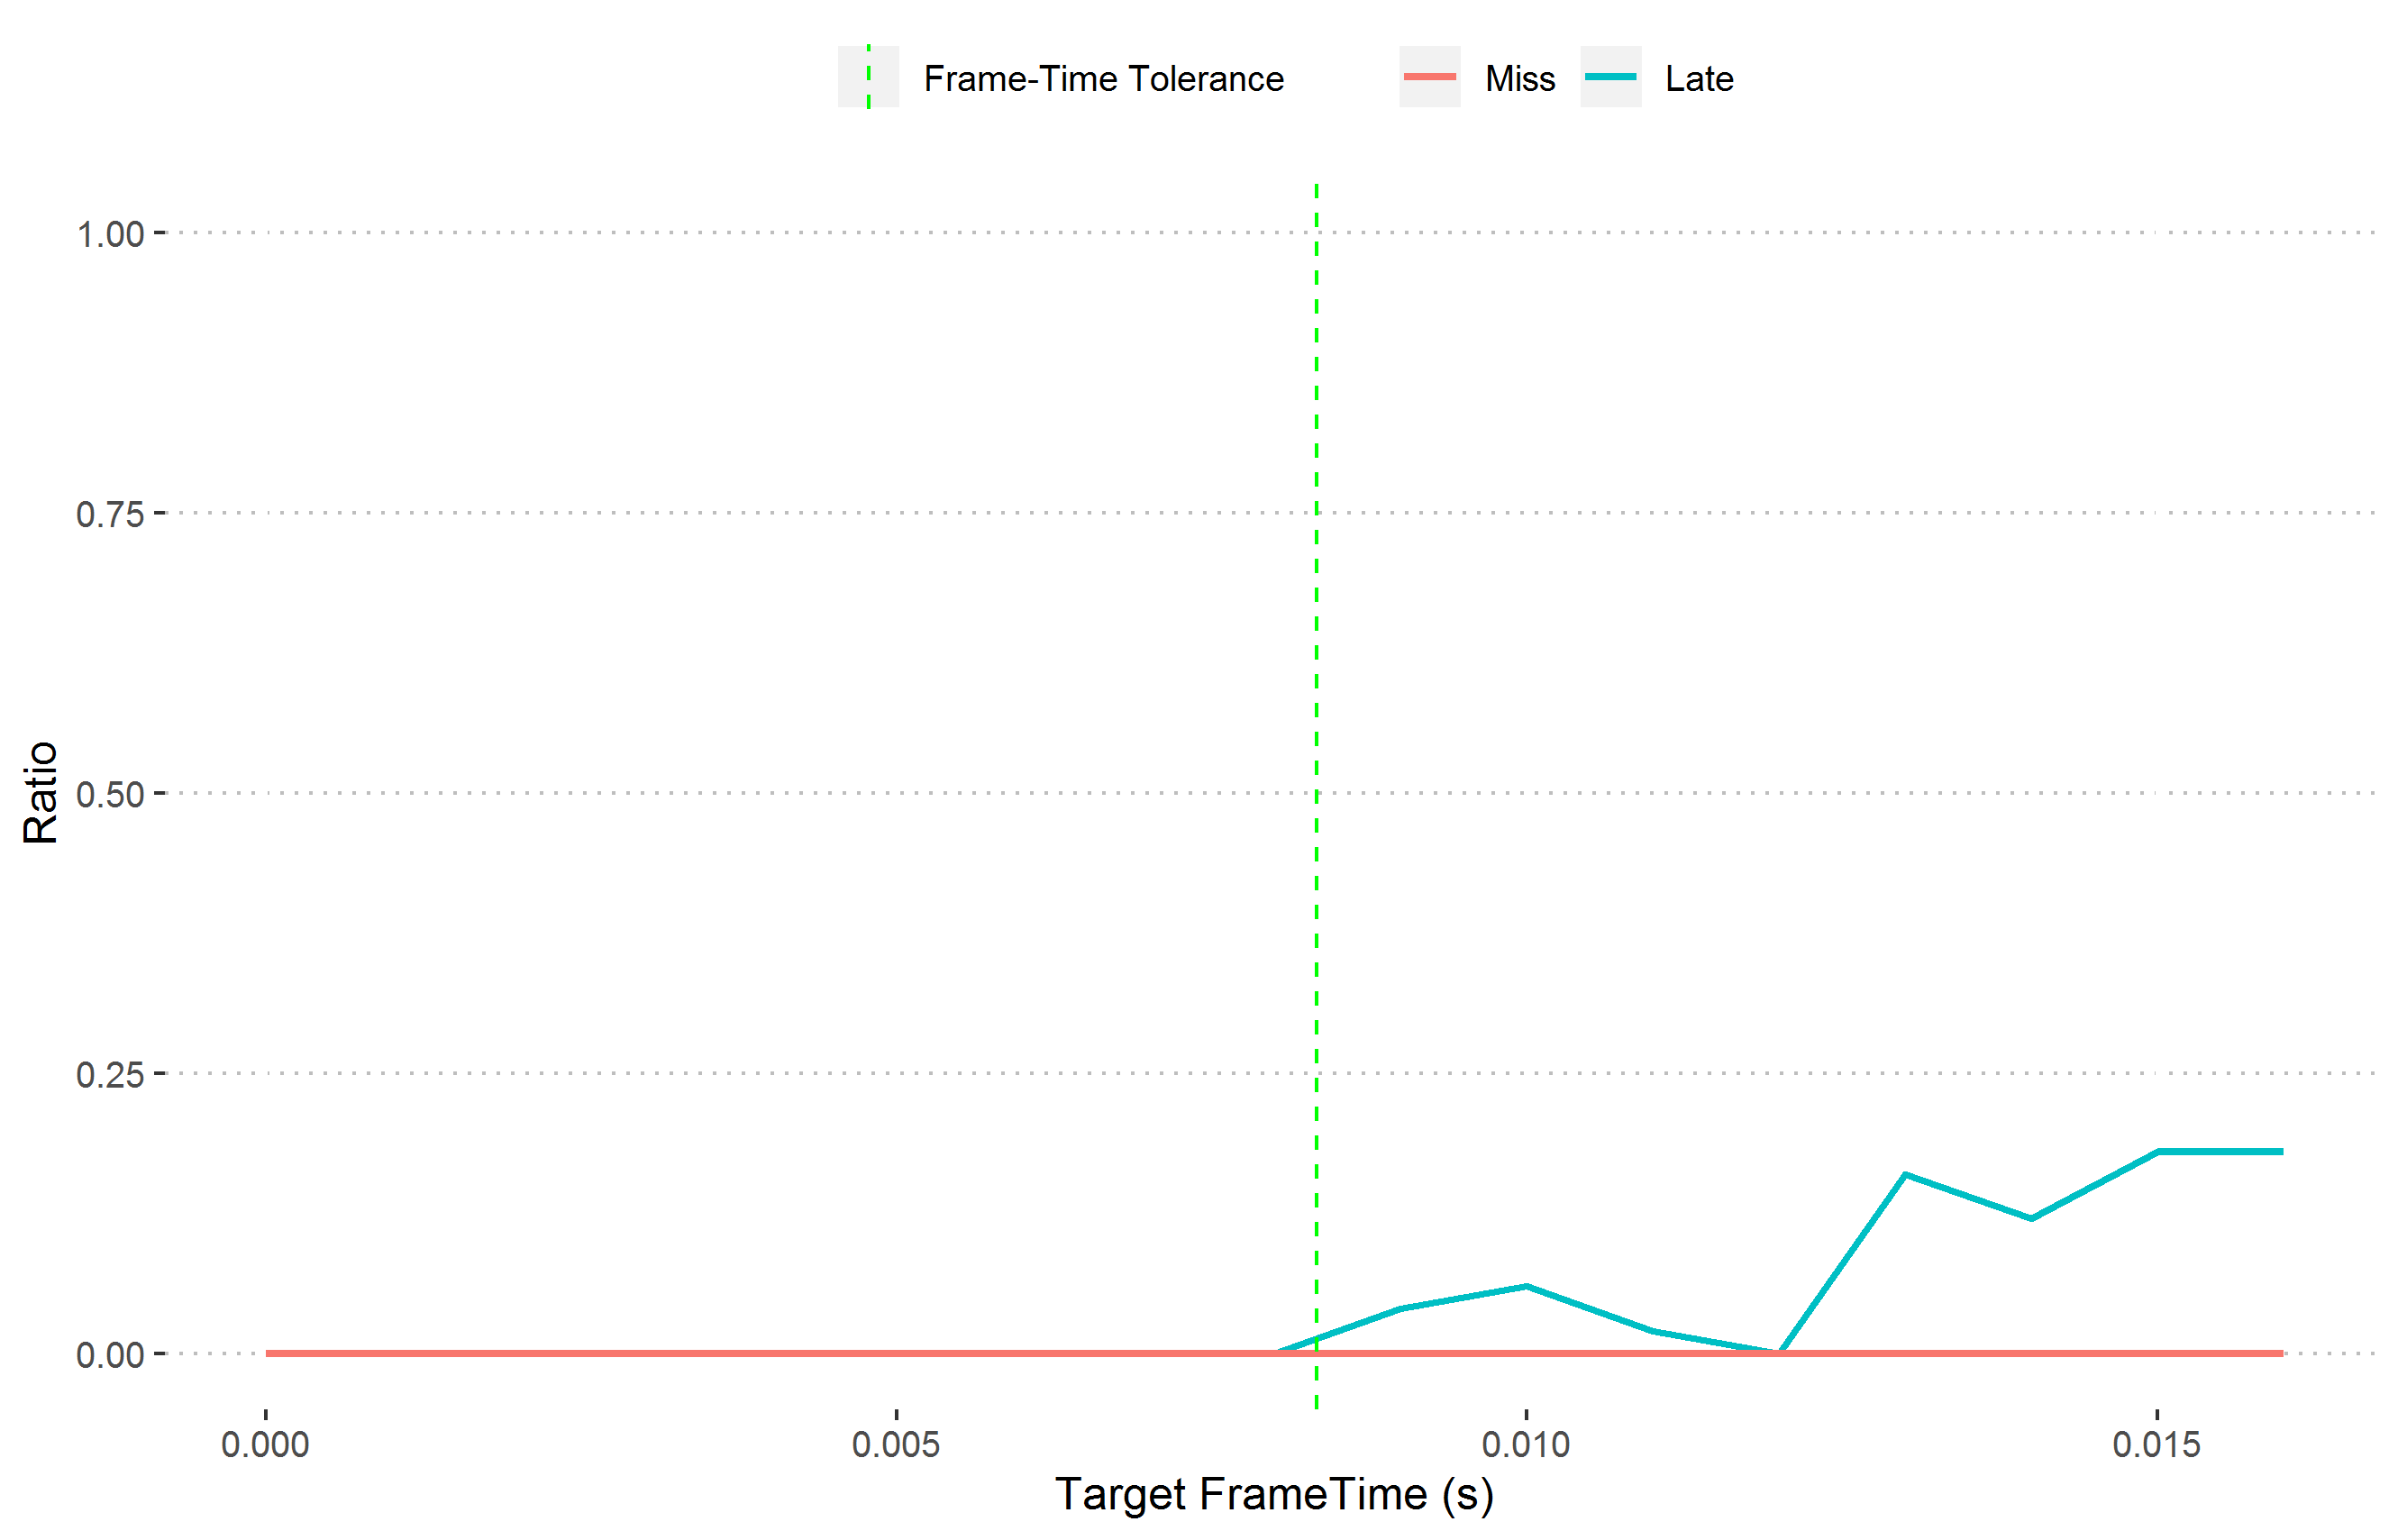
\includegraphics[width=\textwidth]{RatiosVsFrameTimeLow}
	\caption{Ratio of Late to Correct Collisions and Misses to Total Collision vs. frame-time using a frame-time tolerance of $8ms$. The frame-time tolerance is marked in a dashed green line.}
	\label{fig_RatioVsFrameTimeLow}
\end{figure}
\begin{figure}
	\centering
	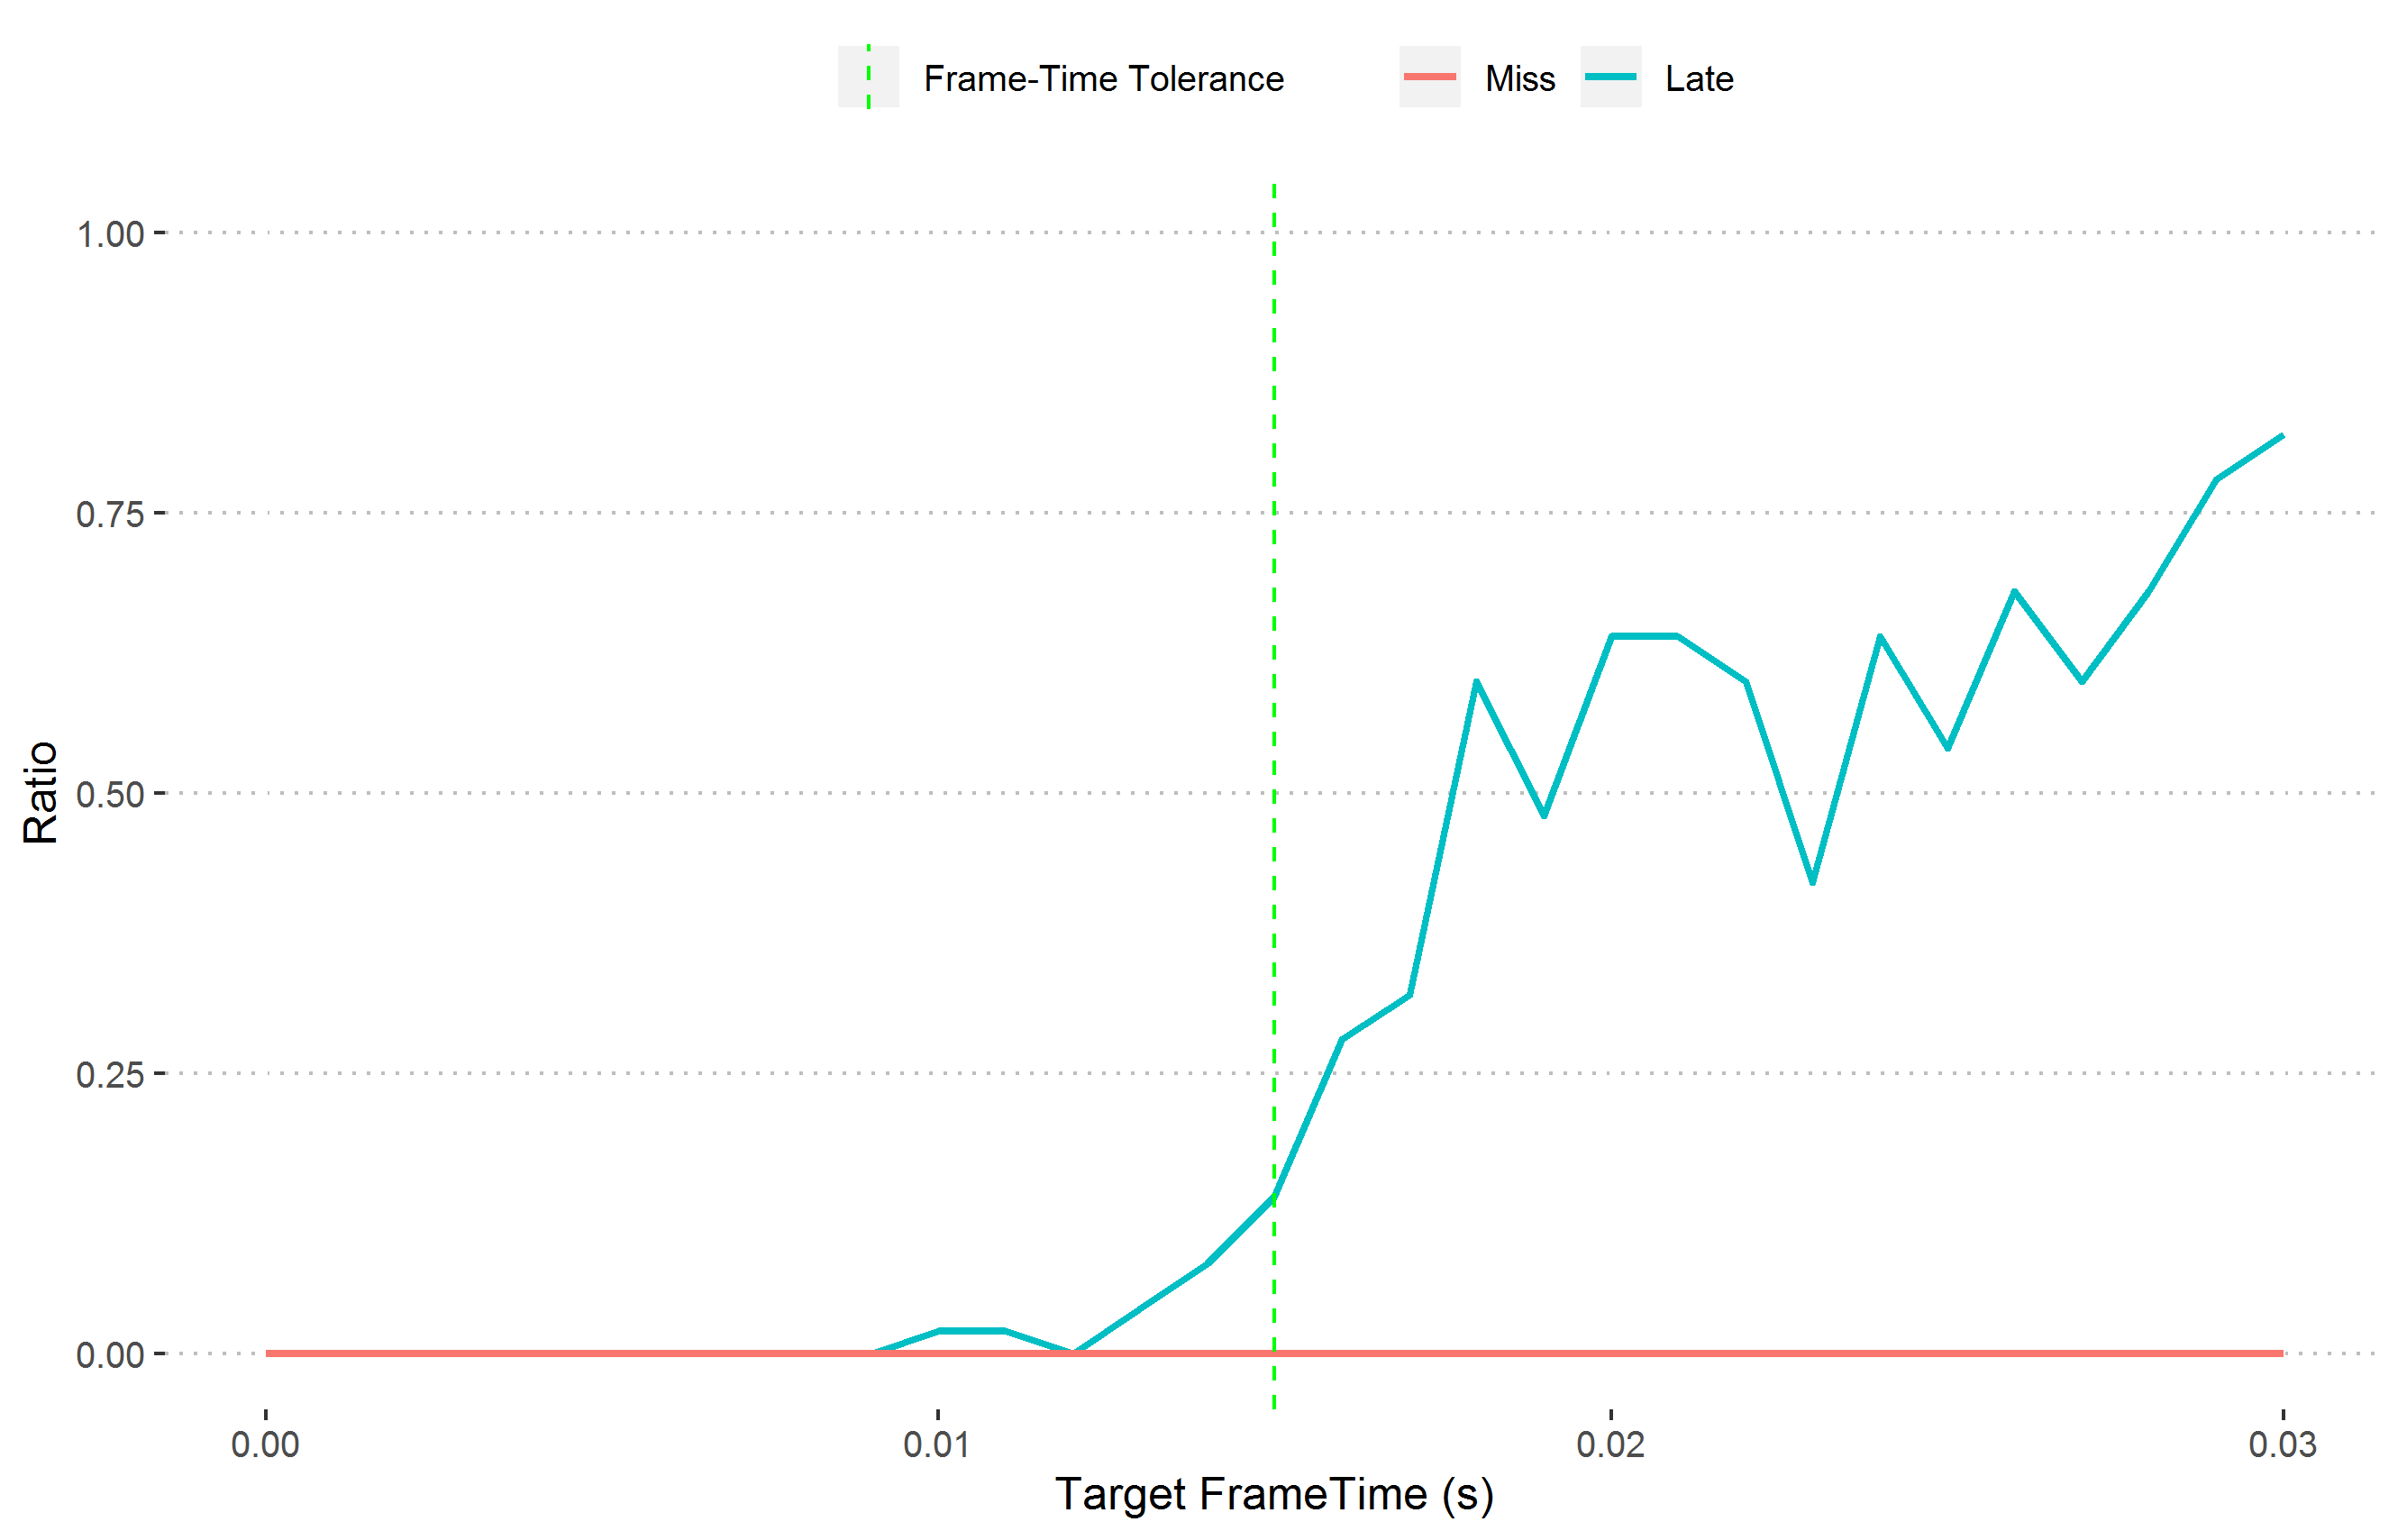
\includegraphics[width=\textwidth]{RatiosVsFrameTimeMid}
	\caption{Ratio of Late to Correct Collisions and Misses to Total Collision vs. frame-time using a frame-time tolerance of $15ms$. The frame-time tolerance is marked in a dashed green line.}
	\label{fig_RatioVsFrameTimeMid}
\end{figure}
\begin{figure}
	\centering
	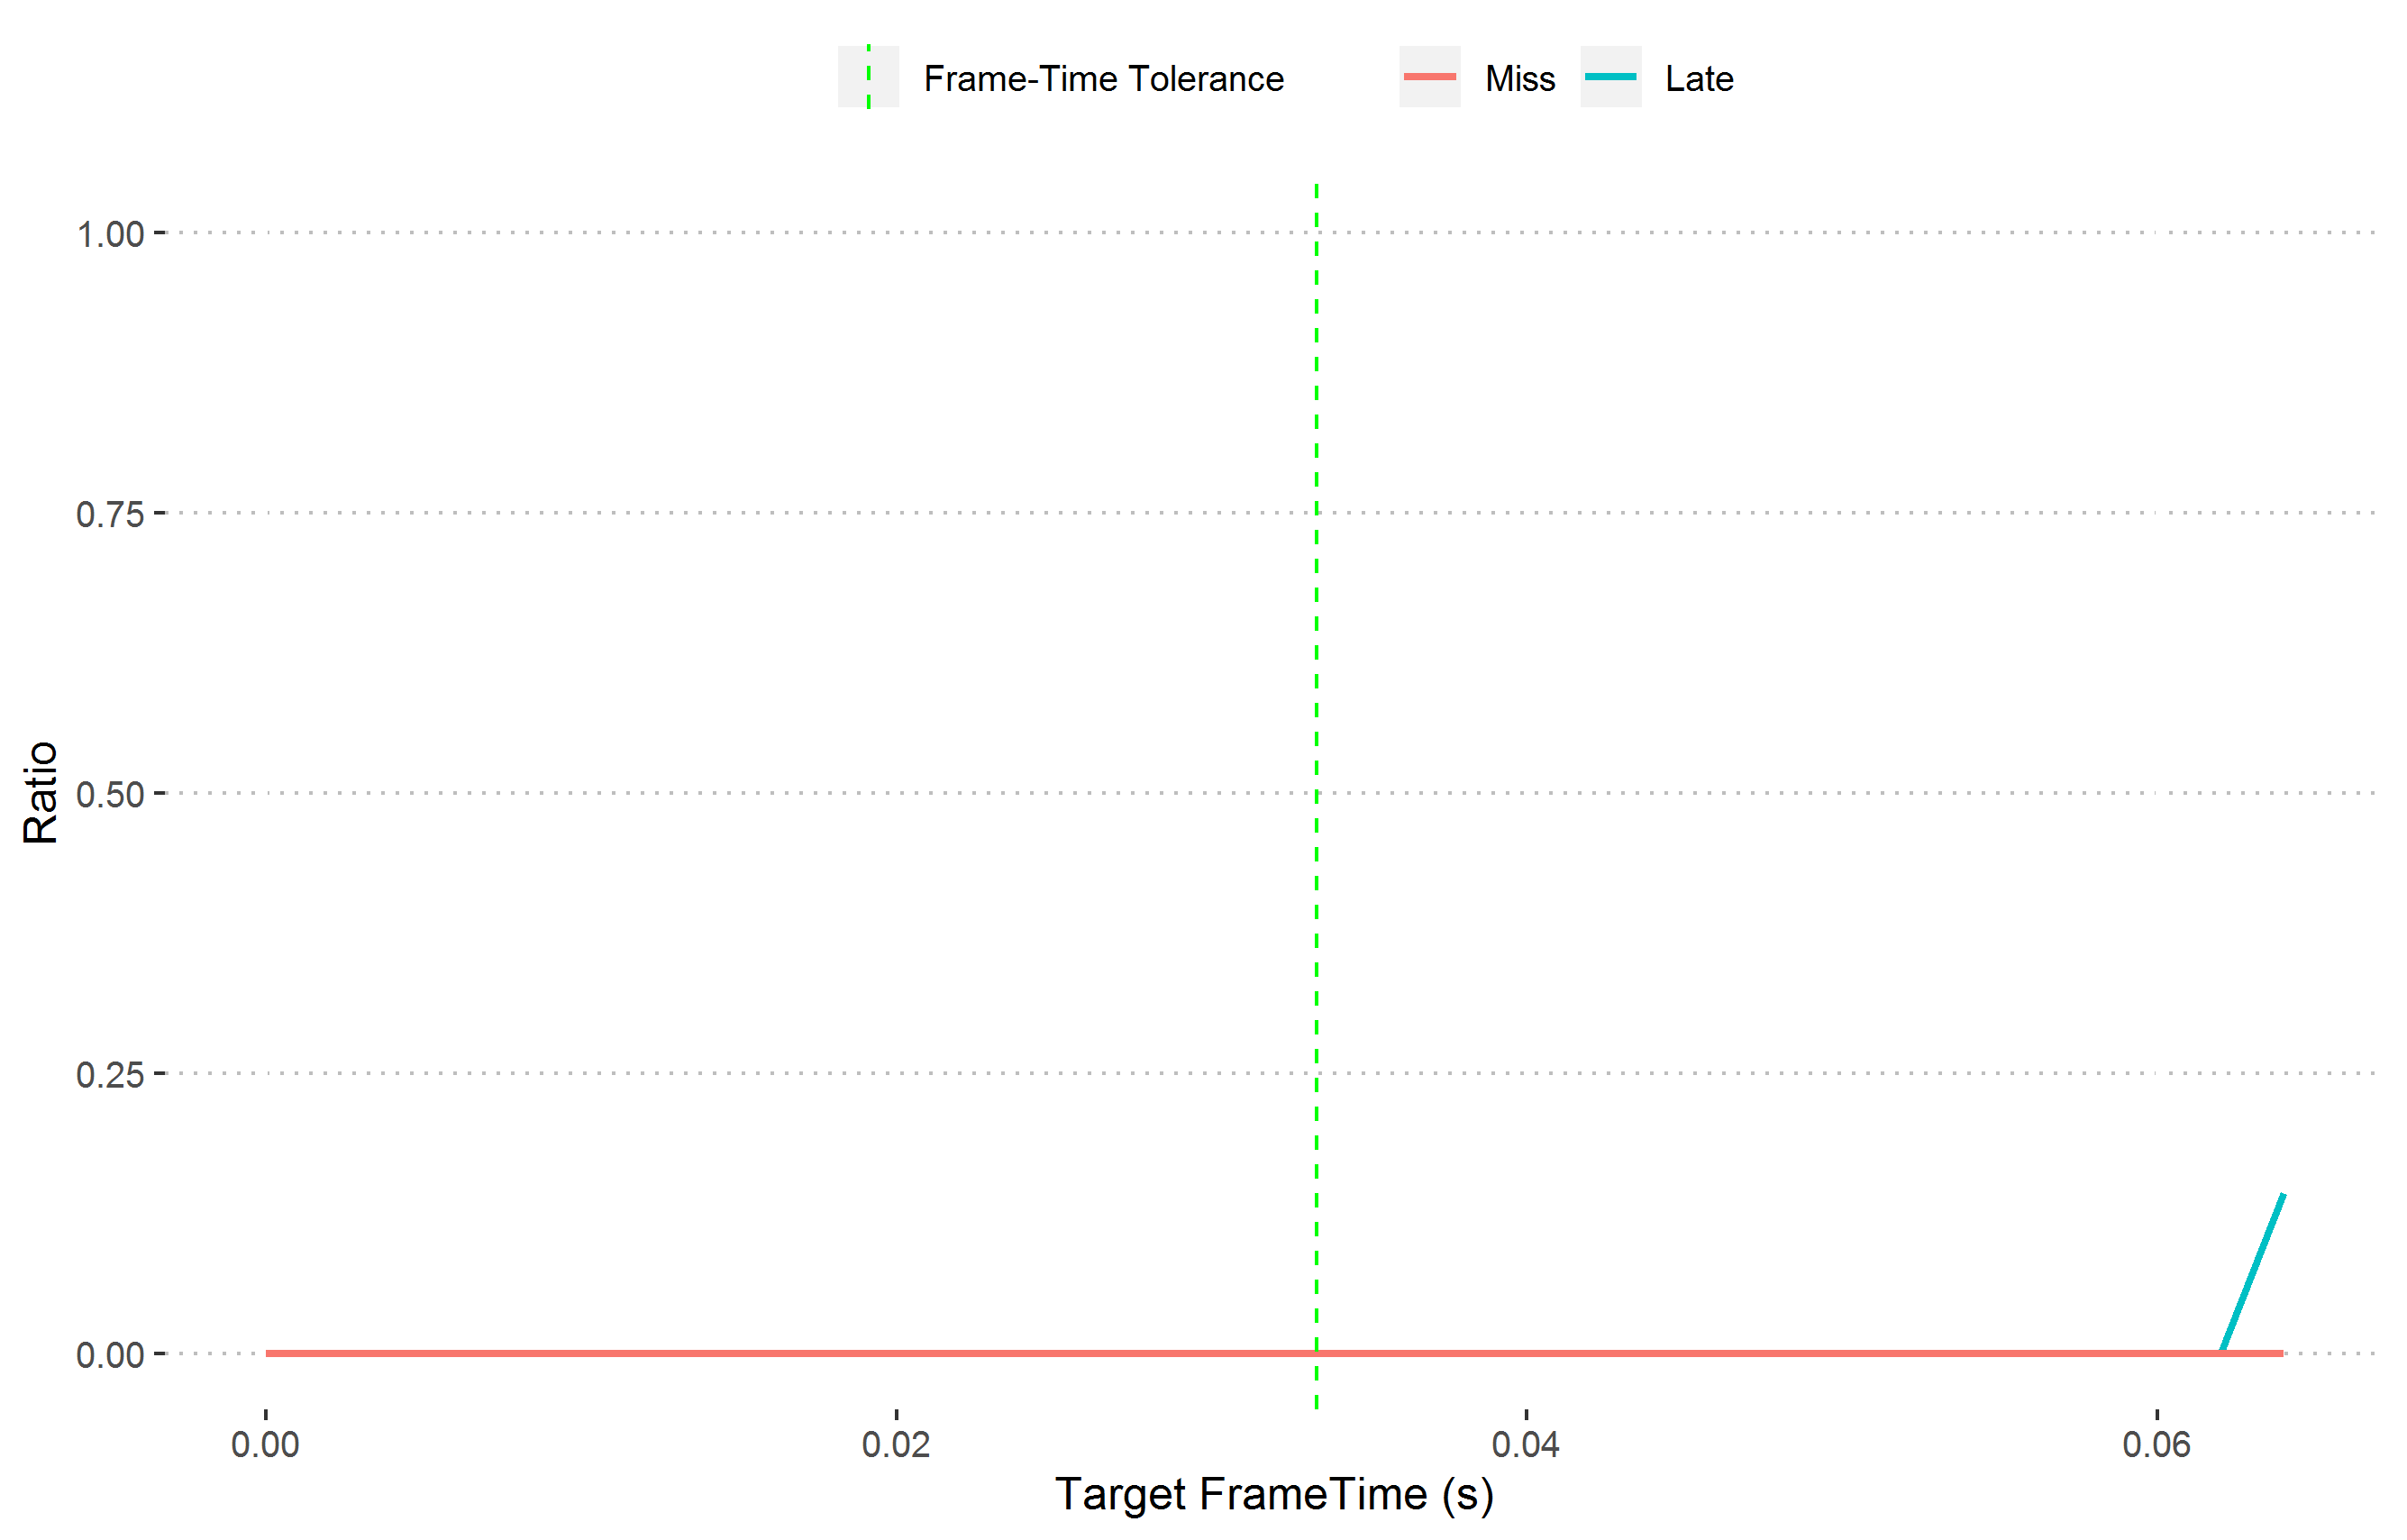
\includegraphics[width=\textwidth]{RatiosVsFrameTimeHigh}
	\caption{Ratio of Late to Correct Collisions and Misses to Total Collision vs. frame-time using a frame-time tolerance of $32ms$. The frame-time tolerance is marked in a dashed green line.}
	\label{fig_RatioVsFrameTimeHigh}
\end{figure}

\begin{figure}
	\centering
	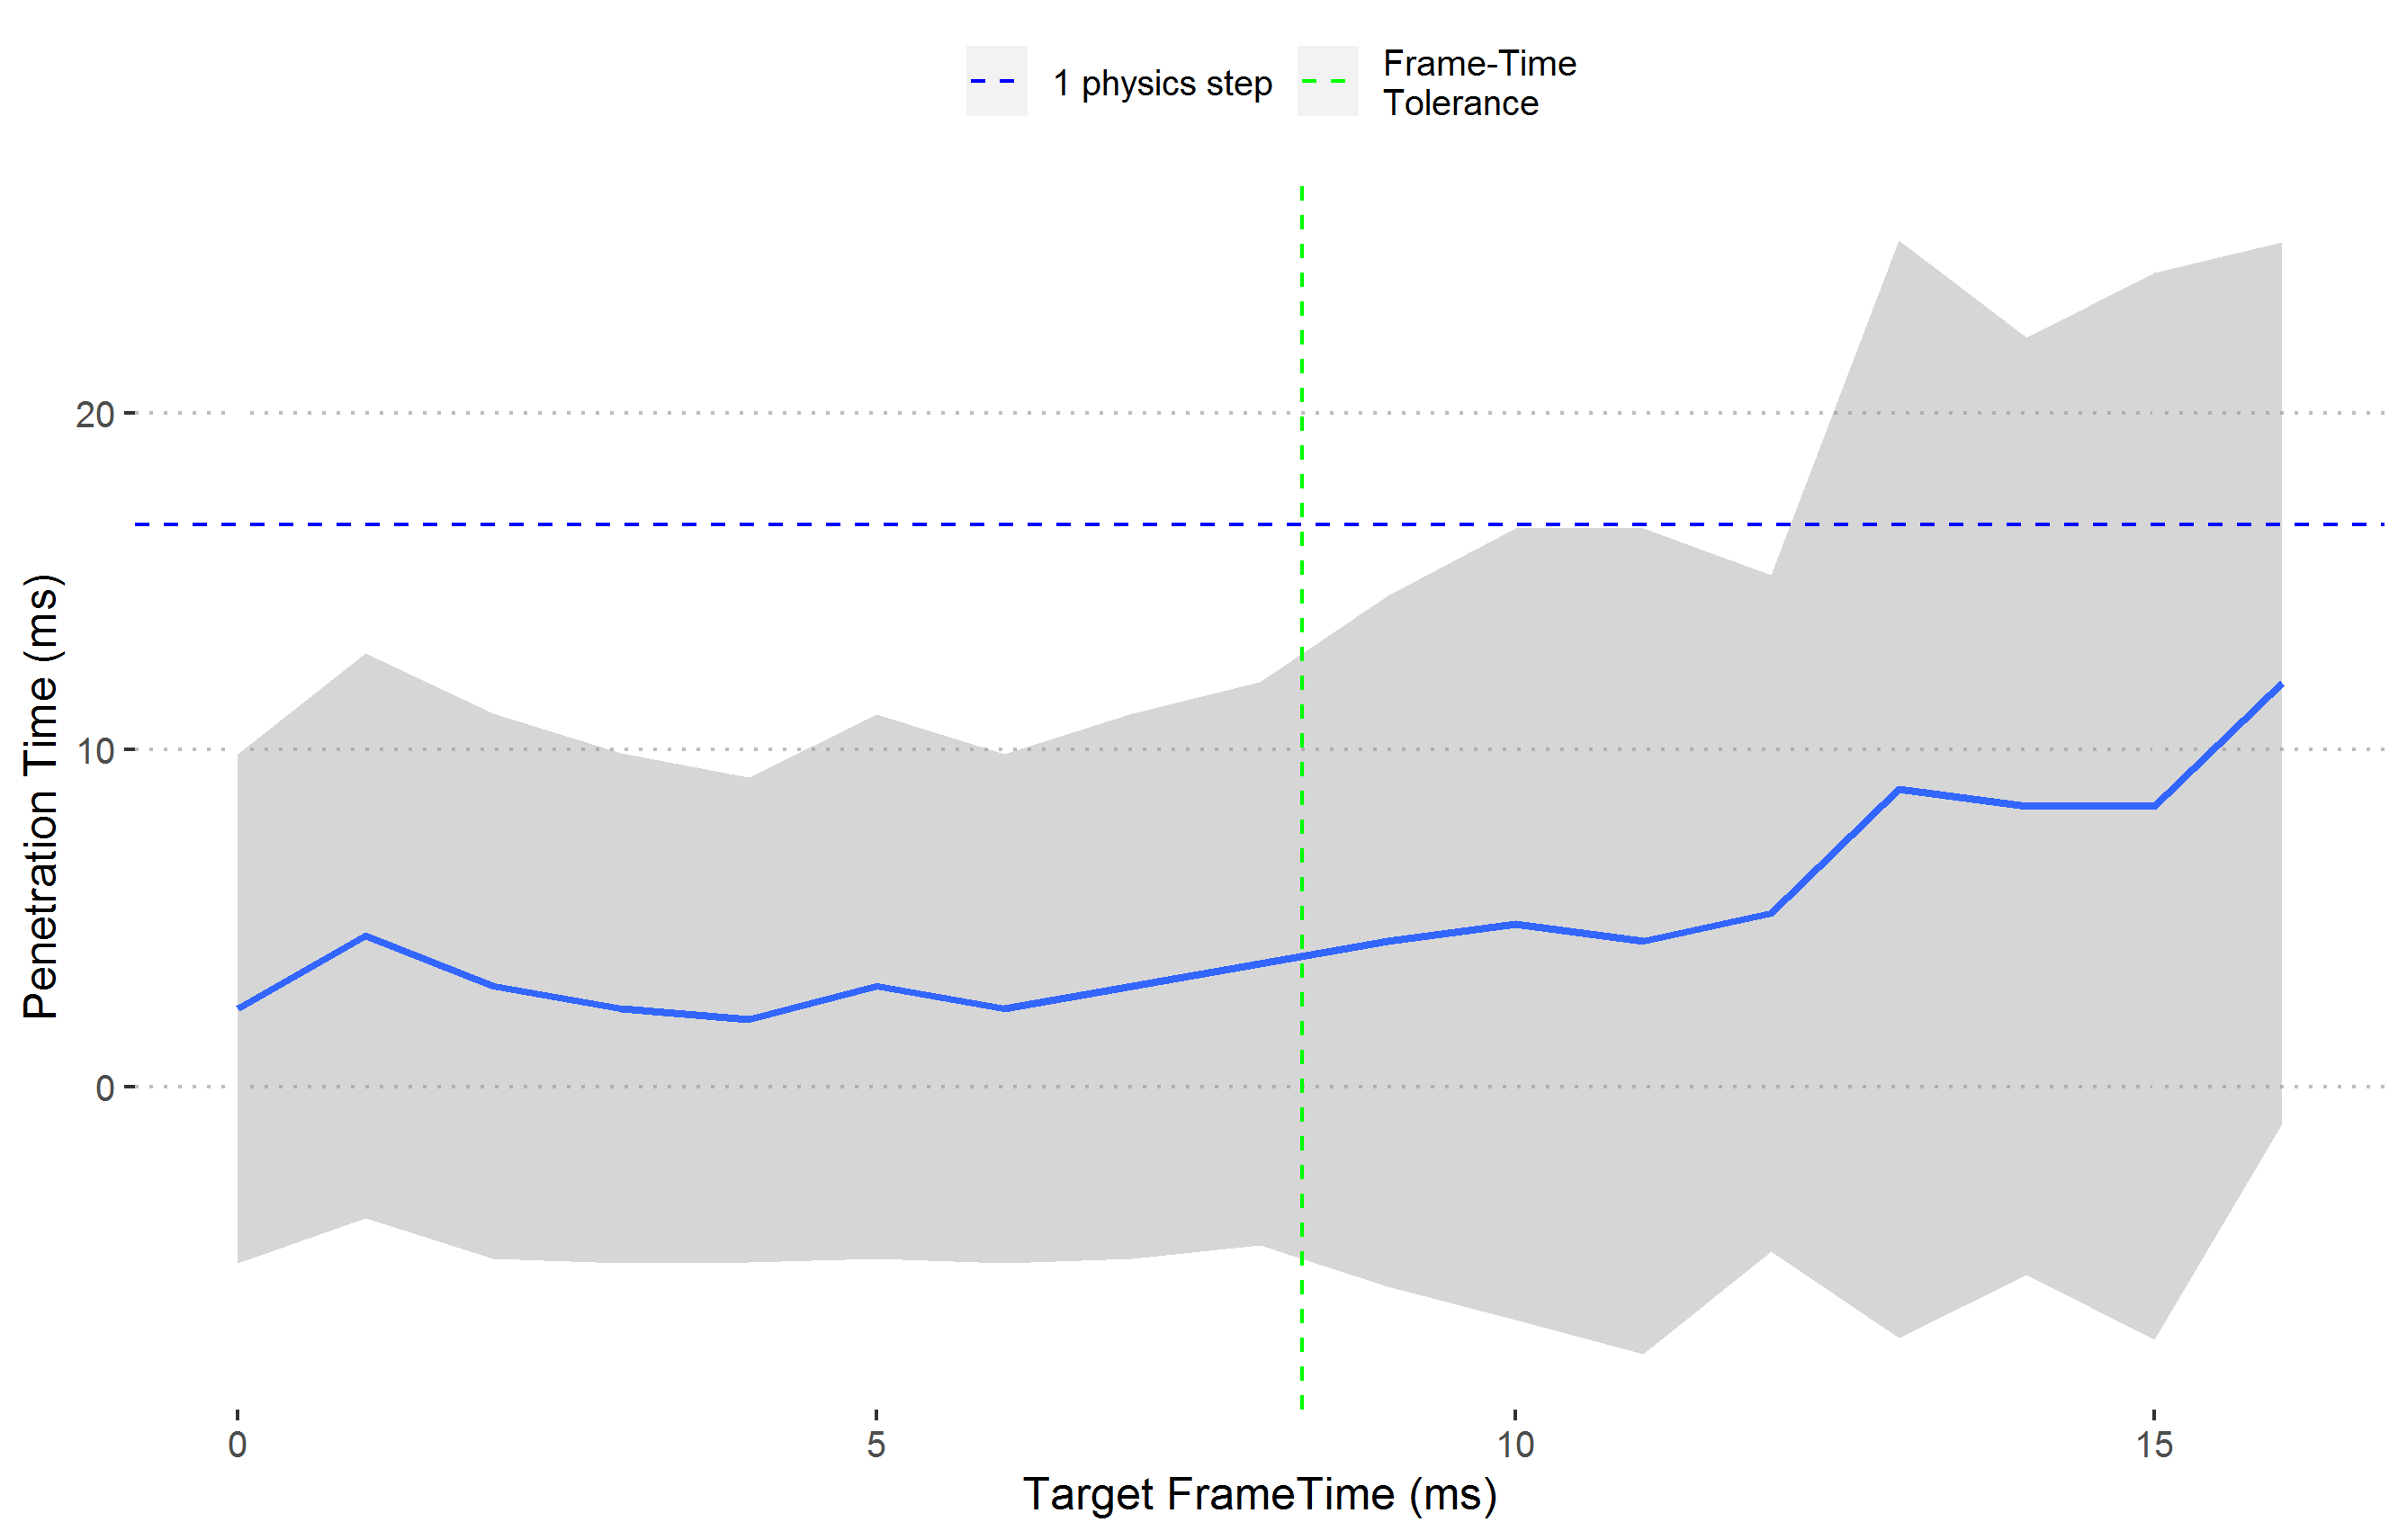
\includegraphics[width=\textwidth]{MeanPenVsFrameTimeLow}
	\caption{Mean penetration time of objects with $+/-2$ standard deviations with varying frame-time using a frame-time tolerance of $8ms$. The maximum expected penetration time of 1 physics step is marked with a dashed blue line. The frame-time tolerance is marked in a dashed green line.}
	\label{fig_CollisionsPenVsFrameTimeLow}
\end{figure}
\begin{figure}
	\centering
	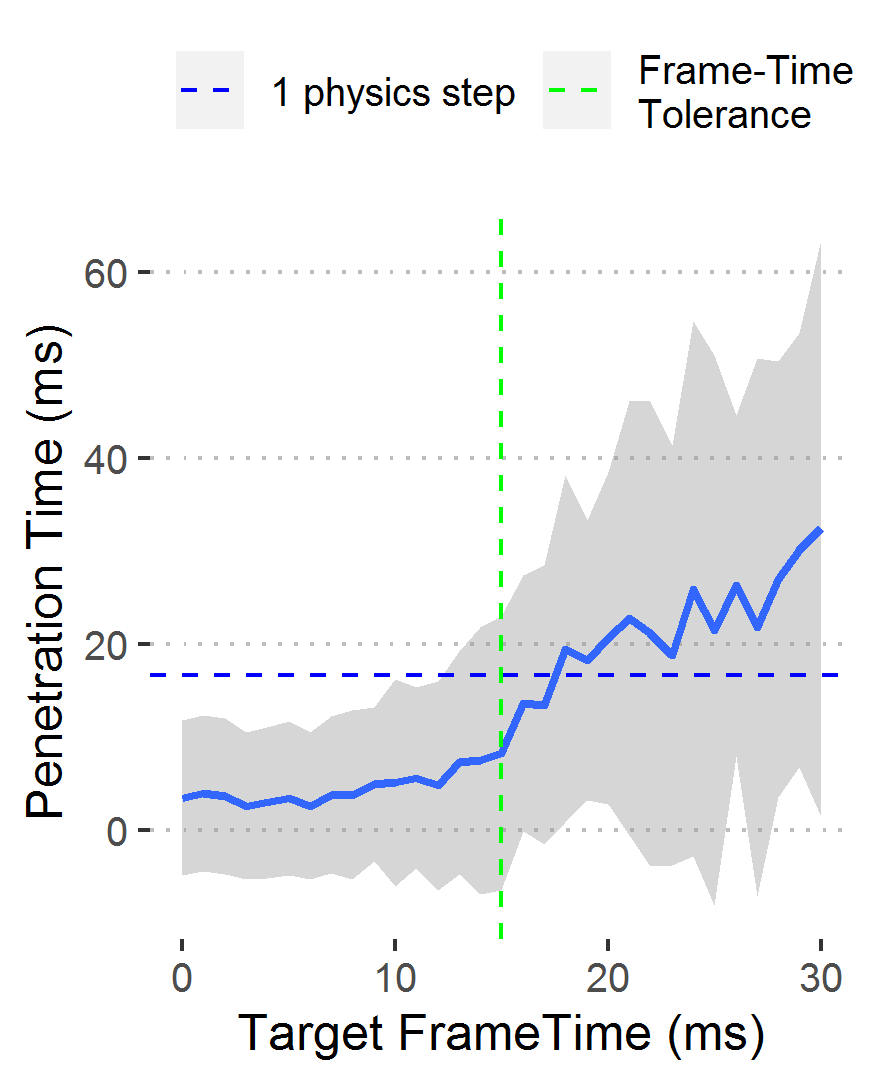
\includegraphics[width=\textwidth]{MeanPenVsFrameTimeMid}
	\caption{Mean penetration time of objects with $+/-2$ standard deviations with varying frame-time using a frame-time tolerance of $15ms$. The maximum expected penetration time of 1 physics step is marked with a dashed blue line. The frame-time tolerance is marked in a dashed green line.}
	\label{fig_CollisionsPenVsFrameTimeMid}
\end{figure}
\begin{figure}
	\centering
	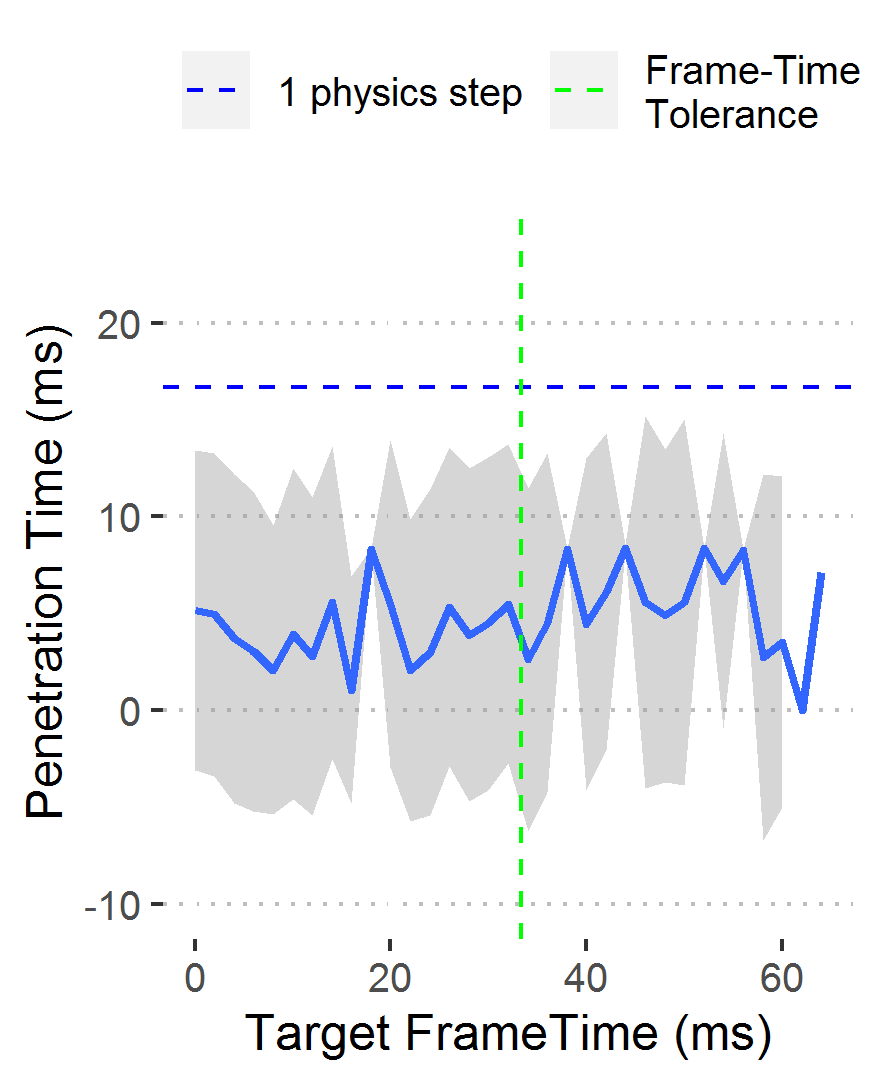
\includegraphics[width=\textwidth]{MeanPenVsFrameTimeHigh}
	\caption{Mean penetration time of objects with $+/-2$ standard deviations with varying frame-time using a frame-time tolerance of $32ms$. The maximum expected penetration time of 1 physics step is marked with a dashed blue line. The frame-time tolerance is marked in a dashed green line.}
	\label{fig_CollisionsPenVsFrameTimeHigh}
\end{figure}

%\begin{figure}
%\centering
%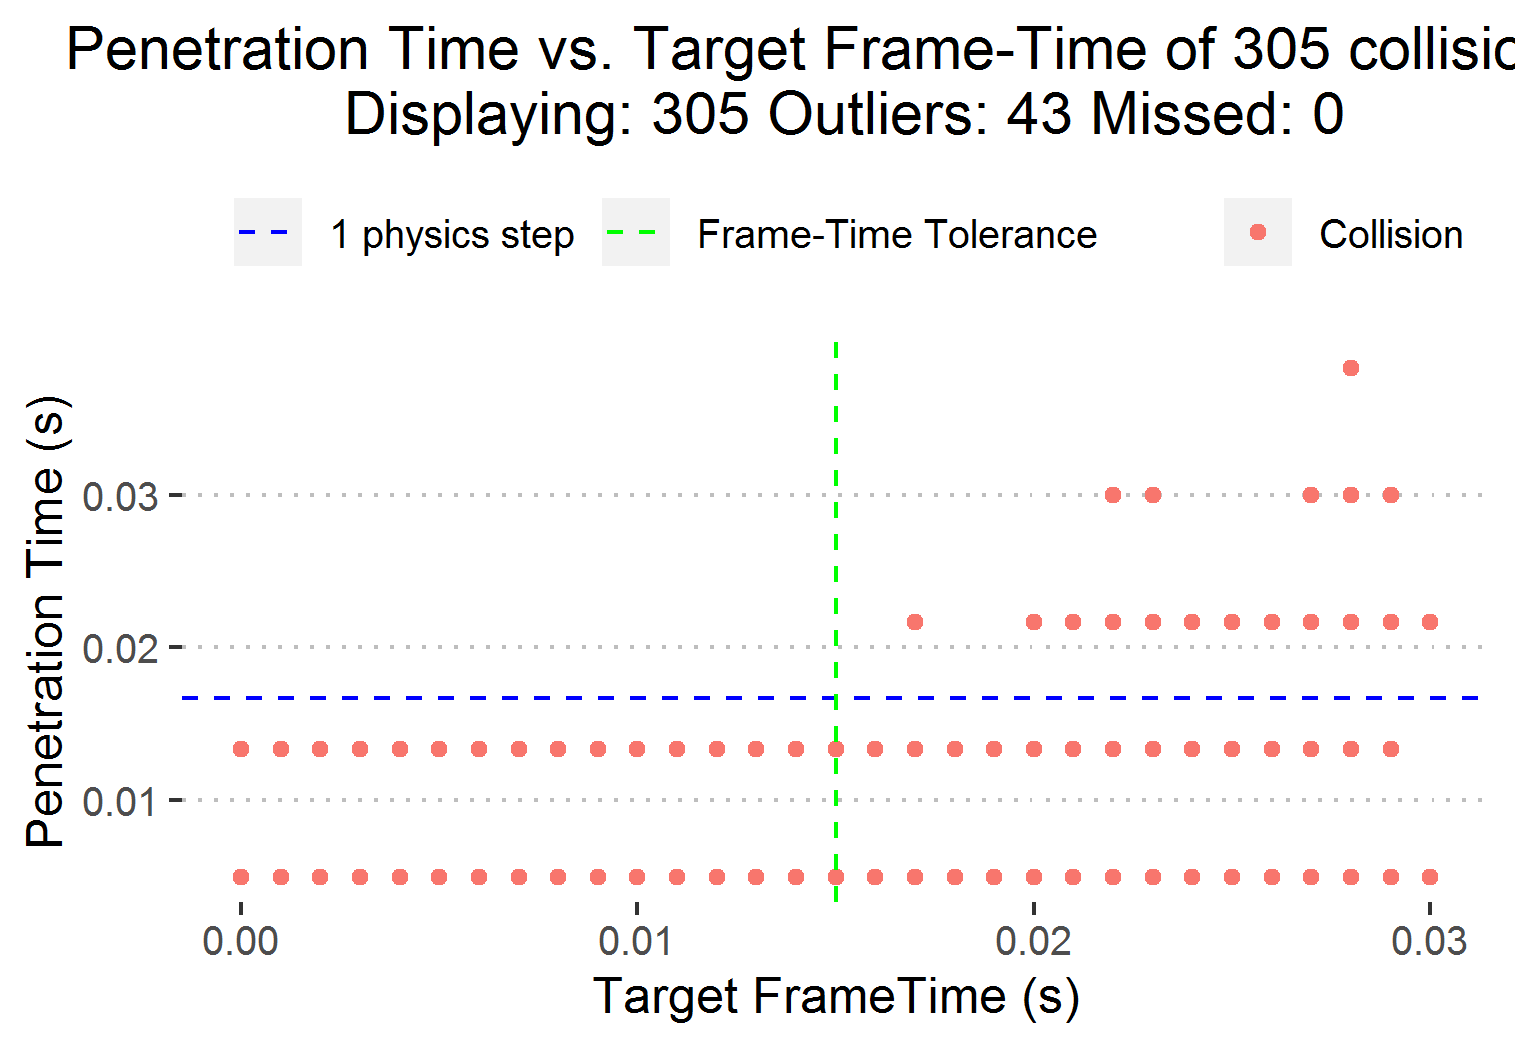
\includegraphics[width=\textwidth]{CollisionsPenVsFrameTime}
%\caption{Penetration time of objects with varying frame-time. Each red point represents one or more collisions. The maximum expected penetration time of 1 physics steps is marked with a dashed blue line. The speed tolerance is marked in a dashed green line. The number and magnitude of errors increases as target frame-time increases beyond the tolerance.}
%\label{fig_CollisionsPenVsFrameTime}
%\end{figure}
%
%\begin{figure}
%\centering
%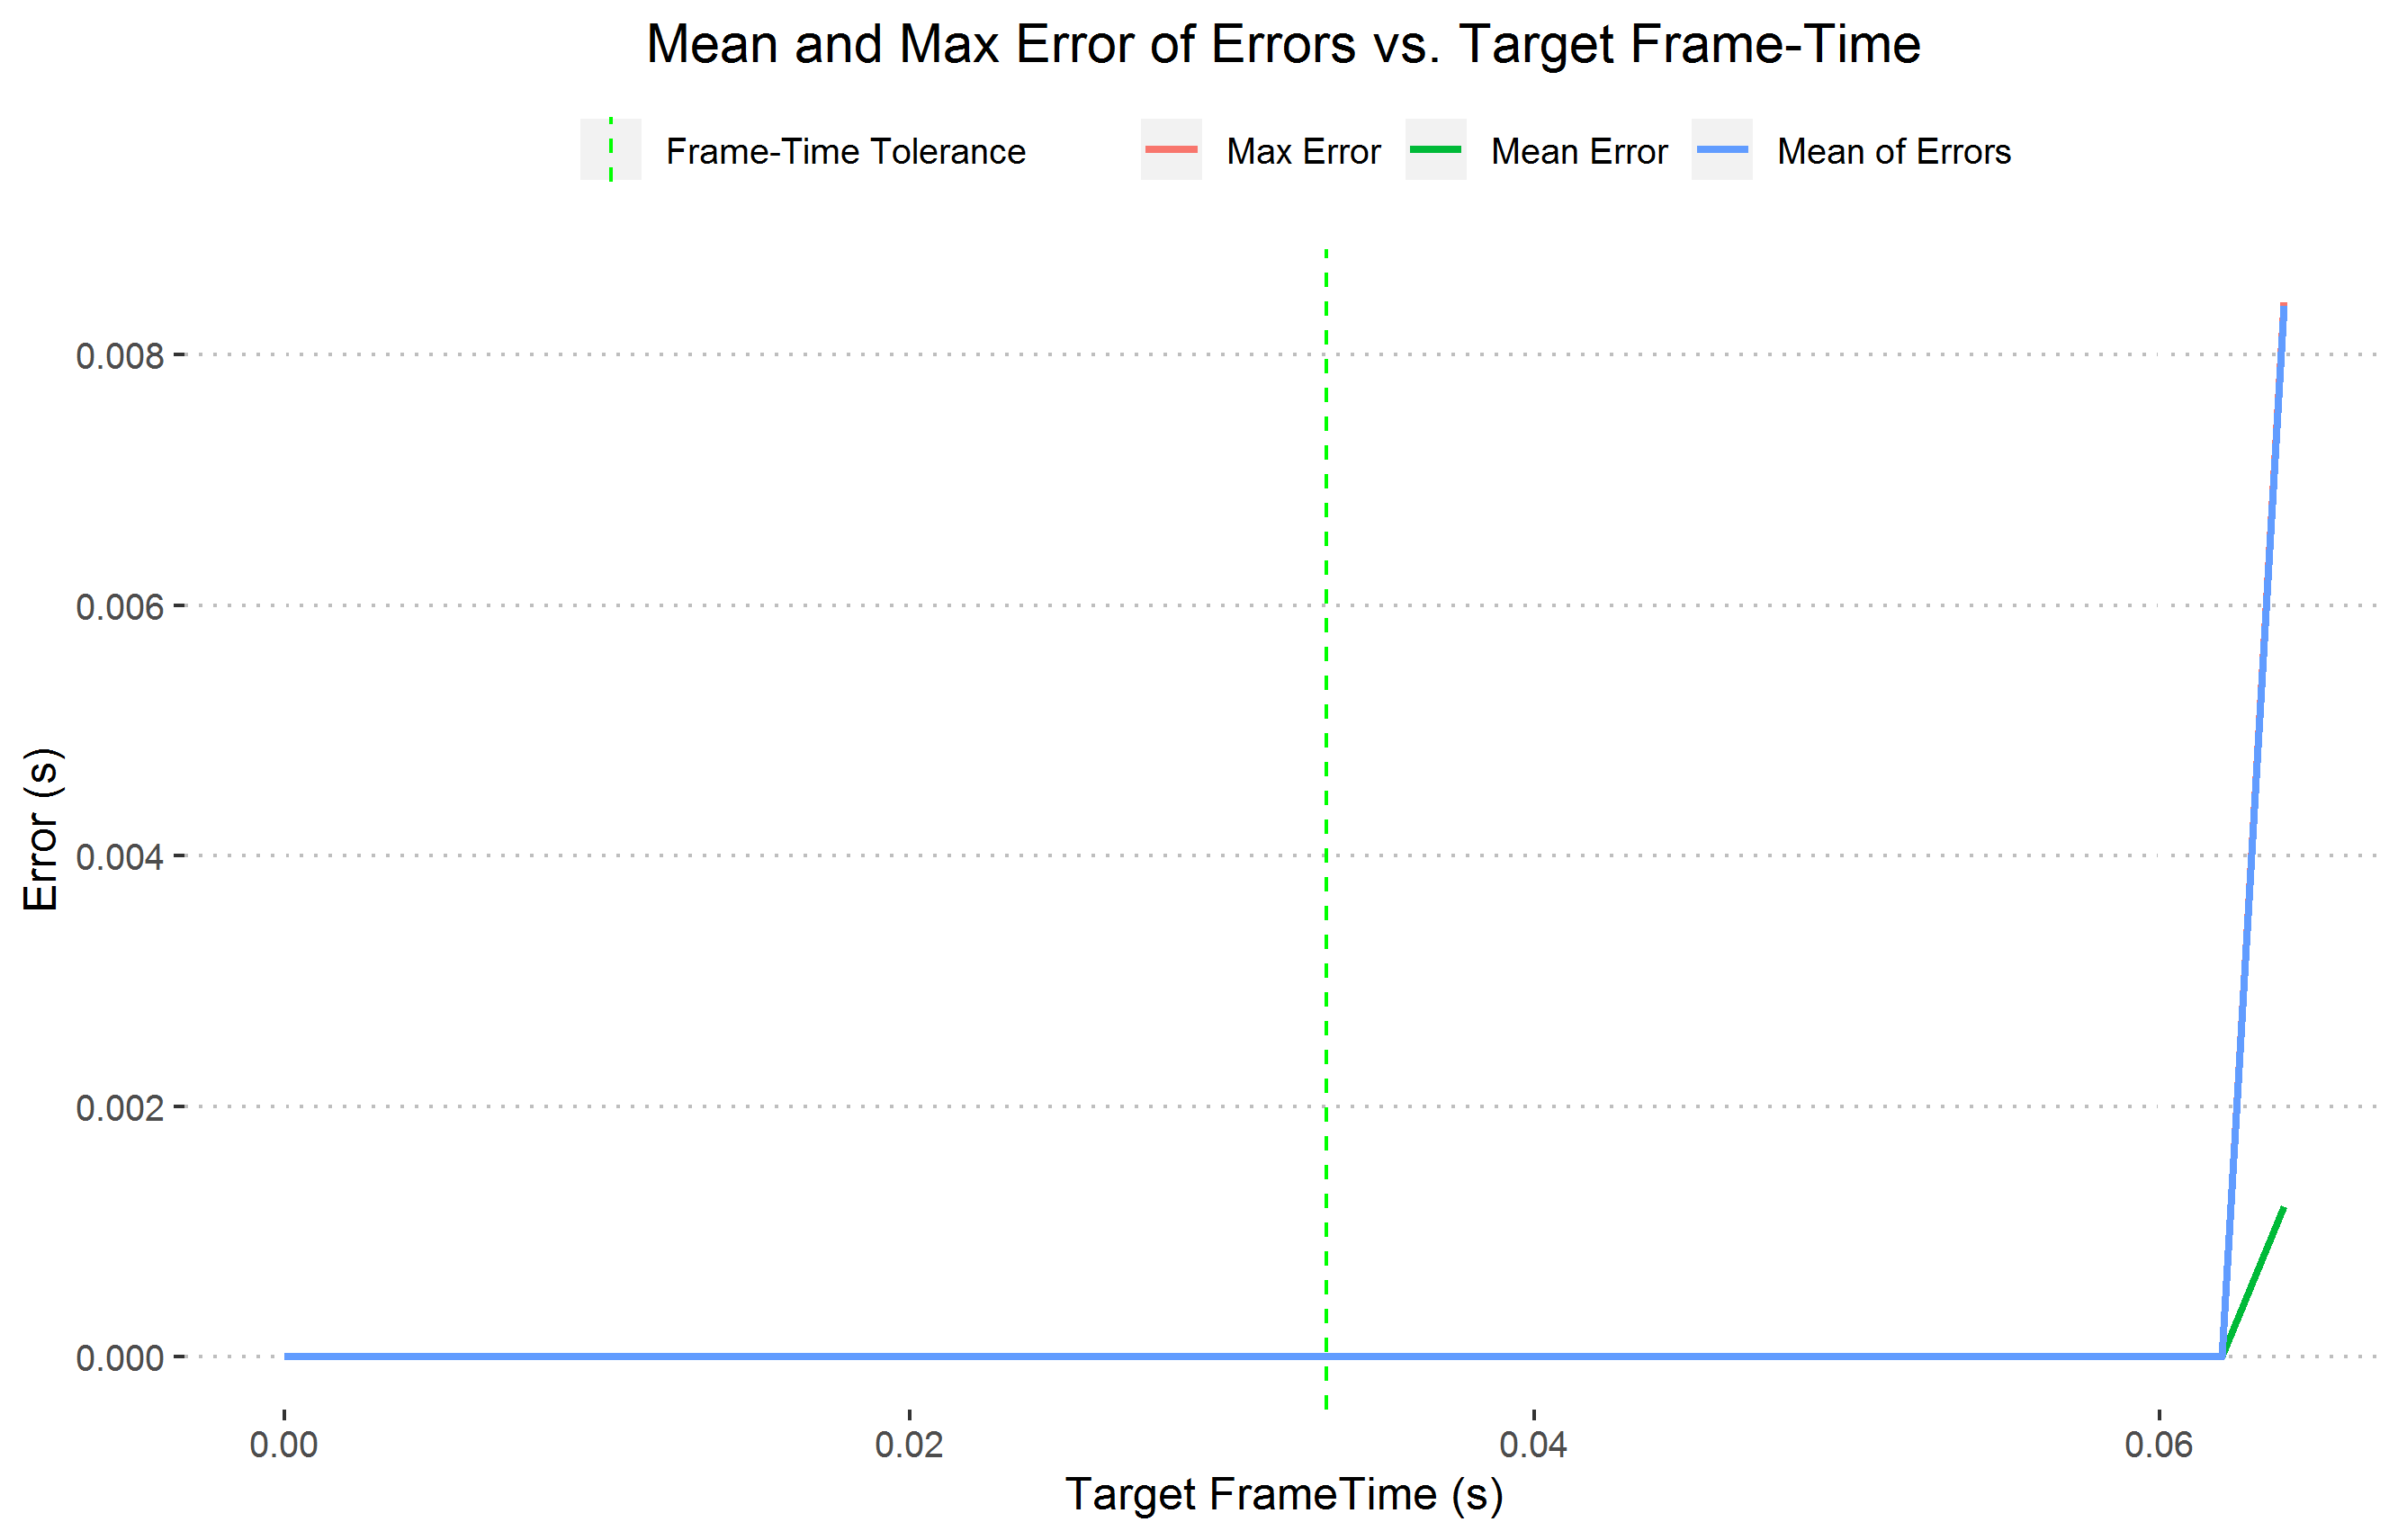
\includegraphics[width=\textwidth]{MeanMaxErrorVsFrameTime}
%\caption{The mean and max of collision errors with varying frame-time}
%\label{fig_MeanMaxErrorVsFrameTime}
%\end{figure}
%
%\begin{figure}
%\centering
%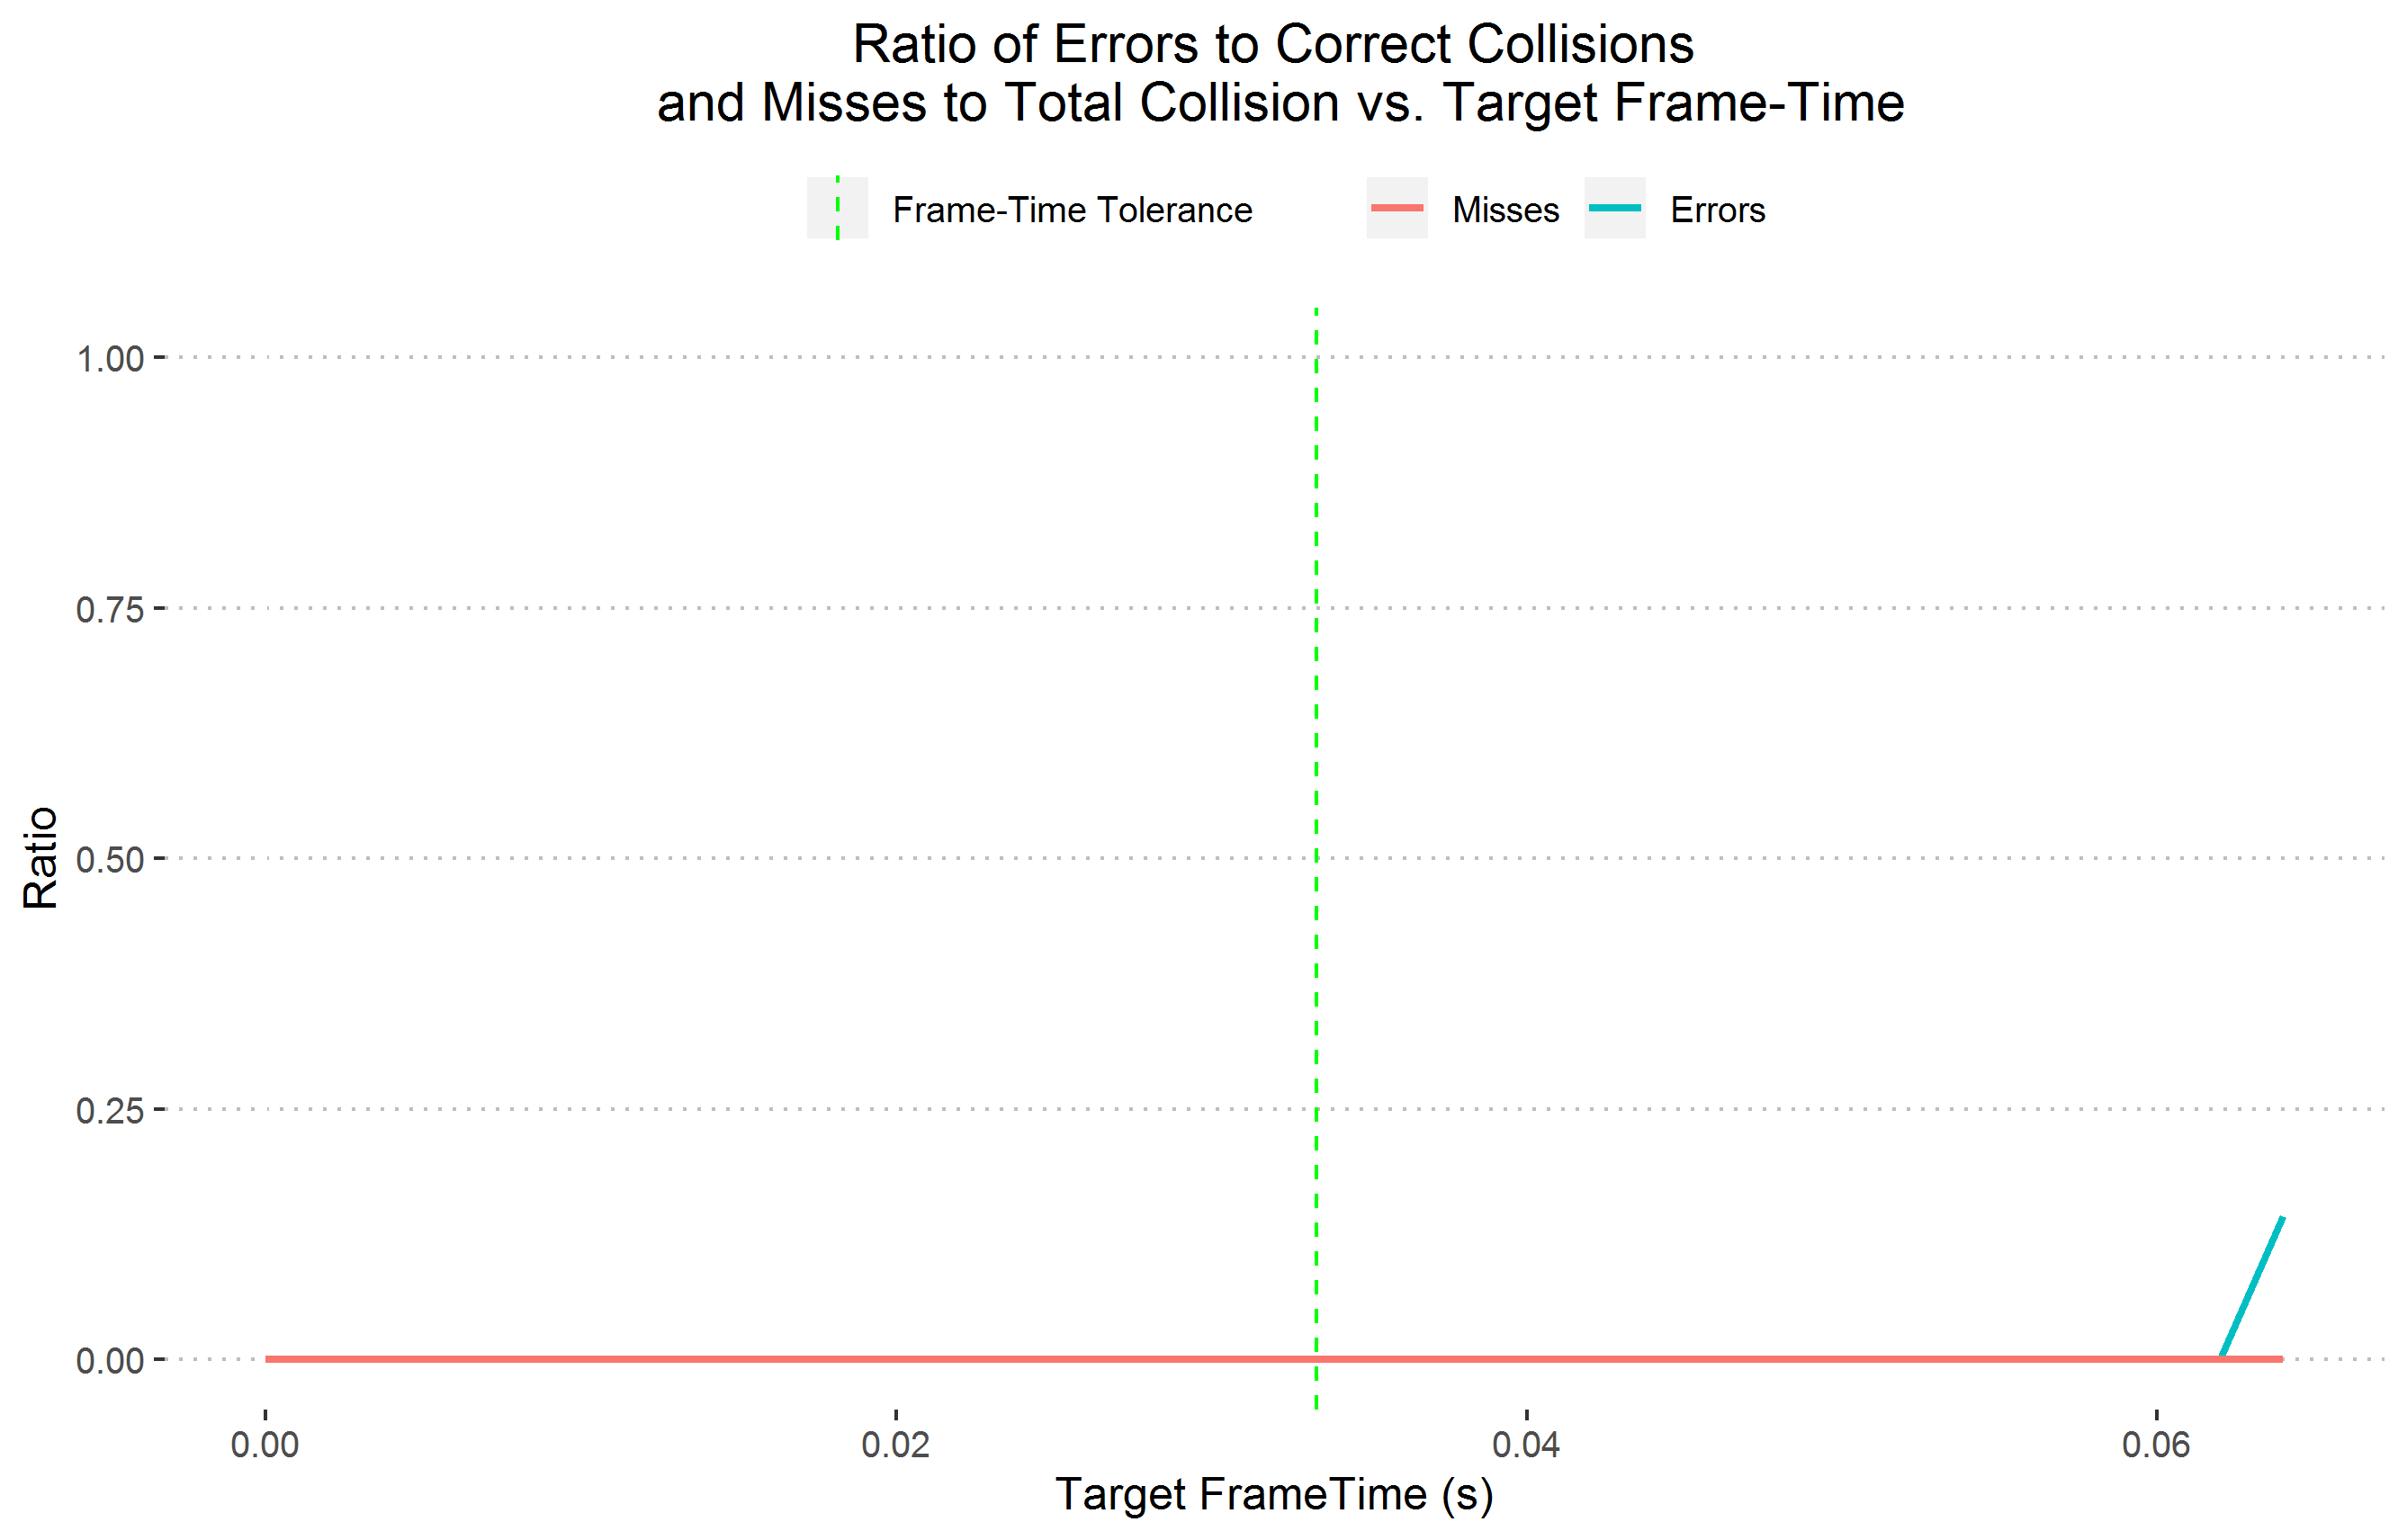
\includegraphics[width=\textwidth]{RatiosVsFrameTime}
%\caption{The ratios of erroneous collisions to correct collisions and missed collisions to total collisions with varying frame-time}
%\label{fig_RatiosVsFrameTime}
%\end{figure}

\begin{table}
	\centering
	\begin{tabular}{llrrrr}
		\toprule
		\multicolumn{1}{l}{Factor} & \multicolumn{1}{l}{Tolerance} & \multicolumn{1}{l}{N} & \multicolumn{1}{l}{Late \%} & \multicolumn{1}{l}{Miss \%} & \multicolumn{1}{l}{Thrashing}  \\ 
		\hline
		Speed      & 16m/s     & 800  & 1     & 0.13       &    0             \\
		Speed      & 32m/s     & 1600 & 0.688 & 0.0422     &    0             \\
		Speed      & 48m/s     & 2372  & 0.632& 0          &    28            \\
		Latency    & 2ms       & 1920  & 10.7 & 0          &    7             \\
		Latency    & 8ms       & 1520  & 0    & 0          &    30            \\
		Latency    & 16ms      & 797  & 2.50  & 0          &    53            \\
		Frame-Time & 8.33ms    & 450  & 0     & 0          &    0             \\
		Frame-Time & 15ms      & 800  & 1.88  & 0          &    0             \\
		Frame-Time & 33.33ms   & 251  & 0     & 0          &    523           \\
		\bottomrule
	\end{tabular}
	\caption{Results summary of collision correctness experiments before the tolerance was exceeded}
	\label{tab_BelowTolerance}
\end{table}

\begin{table}
	\centering
	\begin{tabular}{llrrrr}
		\toprule
		\multicolumn{1}{l}{Factor} & \multicolumn{1}{l}{Tolerance} & \multicolumn{1}{l}{N} & \multicolumn{1}{l}{Late \%} & \multicolumn{1}{l}{Miss \%} & \multicolumn{1}{l}{Thrashing}  \\ 
		\hline
		Speed      & 16m/s     & 800  &   49.9  & 0           & 0               \\
		Speed      & 32m/s     & 1589  &  48.6  & 0           & 11              \\
		Speed      & 48m/s     & 2233  &  45.10 & 1.12        & 167             \\
		Latency    & 2ms       & 1880  &  13.99 & 0           & 0               \\
		Latency    & 8ms       & 1377  &  0.15  & 0           & 121             \\
		Latency    & 16ms      & 574  &   12.20 & 0           & 226             \\
		Frame-Time & 8.33ms    & 400  &   9.50  & 0           & 0               \\
		Frame-Time & 15ms      & 750  &   58.13 & 0           & 0               \\
		Frame-Time & 33.33ms   & 106  &   1.89  & 0           & 693             \\
		\bottomrule
	\end{tabular}
	\caption{Results summary of collision correctness experiments after the tolerance was exceeded}
	\label{tab_AboveTolerance}
\end{table}

In addition to recording the number of collisions that resulted in thrashing, the number of times an object thrashed between servers was also measured. The number of times thrashed is determined by measuring the number of migrations away from the server that the collisions takes place on, before the collision takes place. A histogram of the number of occurrences against the number of times thrashed is shown in Fig. \ref{fig_ThrashingHistogram}. For this histogram, data from the Frame-Time $33.33ms$ experiment is used, as this provides the largest sample of thrashing. Fig. \ref{fig_ThrashingHistogram} demonstrates that the most frequent number of times thrashed is 1, by a large margin followed by a downward trend.

The more times thrashing occurs, the later the collision may be detected as objects continue to be updated and move without a collision occurring. It should be noted that thrashing occurring does not guarantee that a late collision will take place. The more times thrashing takes place, the more physics updates occur and the further the objects may be moved towards (and eventually overlapping) each other. Therefore, a greater number of times thrashed, means a late and incorrect collision response is more likely, but not guaranteed.

\begin{figure}[t]
	\centering
	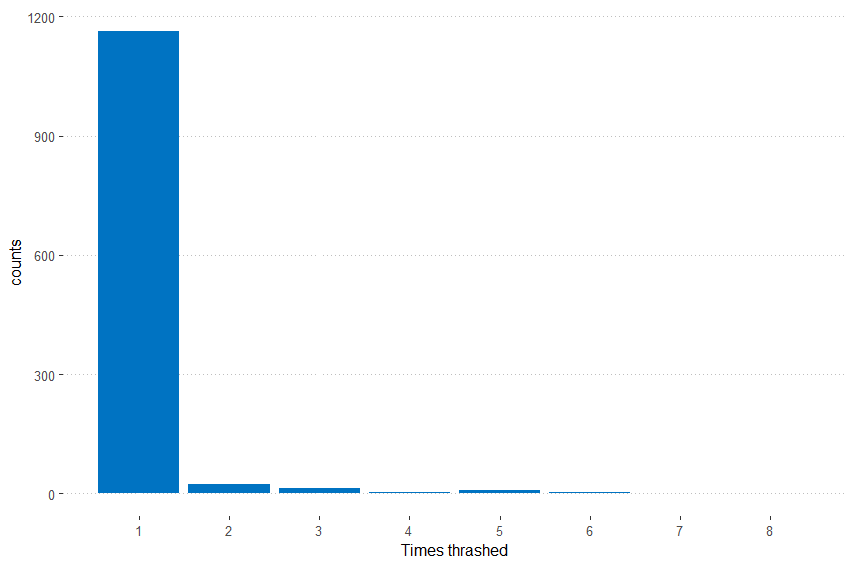
\includegraphics[width=\textwidth]{ThrashingHistogram}
	\caption{Thrashing Histogram. The number of occurrences vs the number of times thrashed.}
	\label{fig_ThrashingHistogram}
\end{figure}

\subsection{Experiment- Varying Factors Evaluation}
As the speed increases, the proportion of late collisions to correct collisions increases, as shown in Figs. \ref{fig_RatioVsSpeedLow}, \ref{fig_RatioVsSpeedMid} and \ref{fig_RatioVsSpeedHigh}. When speed is below the speed tolerance, late collisions do not exceed 10\%. This 10\% is assumed to be caused by false-positives. Once above the speed tolerance, the proportion of late collisions increases immediately, which is predicted by the aura calculation. Missed collisions begin to occur when speed exceed $80ms^{-1}$ in the $48ms^{-1}$ experiment, this is due to objects travelling so quickly, the objects completely pass one another, missing the collision entirely.

It should also be noted that object speed is application specific and objects need to be travelling directly towards the centre of each other and one of the objects has to be travelling above the tolerance speed, in order for errors to occur.

As the speed increases, the mean penetration time increases, as shown in Figs. \ref{fig_CollisionsPenVsSpeedLow}, \ref{fig_CollisionsPenVsSpeedMid} and \ref{fig_CollisionsPenVsSpeedHigh}. With the exception of the starting speed, the standard deviation remains constant below the tolerance line. Once speed increases above the tolerance line, the standard deviation initially increases, but appears to remain constant after the initial increase. 
%Note that the mean error increases in discrete steps (with some small variation), this is due to the discrete physics time-steps.

As the latency increases, the proportion of late collisions to correct collisions increases, as shown in Fig. \ref{fig_RatioVsLatencyHigh}. However, Figs. \ref{fig_RatioVsLatencyLow} and \ref{fig_RatioVsLatencyLow} do not show this relationship. In the $2ms$ latency tolerance experiment, late collisions do not exceed $20\%$, which is assumed to be accounted for by false-positives. The aura calculation predicts that late collisions should start occurring once $3ms$ has been exceeded, however, this is not observed, as the proportion does not increase above what would be expected for false-positives.
In the $8ms$ latency tolerance experiment, late collisions do not exceed $2\%$, which is assumed to be accounted for by false-positives. This remains the case even when the tolerance is exceeded. The aura calculation predicts that late collisions will not begin to occur until $20ms$ latency is reached, which this experiment does not reach, therefore no late collisions outside of false-positives are expected. In the $16ms$ latency tolerance experiment, late collisions do not exceed $3\%$ below the tolerance, which is assumed to be accounted for by false-positives. The aura calculation predicts that late collisions will not begin to occur until $20ms$ latency is reached. In Fig. \ref{fig_RatioVsLatencyHigh} we see the proportion of errors increase from $20ms$ and above, however, it does not exceed the expected false-positive proportion until $25ms$ latency is reached.
%TODO: Re-run latency experiment, larger sample size?

%When latency is below the latency tolerance, late collisions do not exceed 10\%. This 10\% can be accounted for by false-positives. Once above the speed tolerance, the proportion of late collisions increases immediately, which is predicted by the aura calculation.

As latency increases standard deviation remains constant below the tolerance value, as shown in Figs. \ref{fig_CollisionsPenVsLatencyLow}, \ref{fig_CollisionsPenVsLatencyMid} and \ref{fig_CollisionsPenVsLatencyHigh}. With only a small number of exceptions (in $2ms$ experiment), the mean $+2$ standard deviations does not exceed the maximum expected penetration when below the latency tolerance. Above the latency tolerance value, the standard deviation increases for the $16ms$ tolerance experiment, but remains constant for the first two latency experiments. In addition, the first two experiments do not show a clear increase in mean penetration, this is due to the aura calculation's discrete nature and as $15ms$ has been used for the frame-time tolerance, small increases in latency of $2$ and $8ms$ will not show the increase in error to the next discrete step. However, in the final experiment using $16ms$, the relationship of increasing penetration as latency increases is demonstrated.

The $2ms$ latency tolerance experiment exhibits more false-positives than the other experiments, including across the entire range of values used. This may be a result of small aura sizes producing more false-positive, the sample size being to small or another unknown effect which has not been accounted for. In addition, although late collisions increase as actual latency exceeds $20ms$ in the $15ms$ tolerance experiment, the mean $+2$ standard deviations does not exceed the maximum expected penetration line until $26ms$ actual latency is reached. Both of these unexpected results should be investigated further in the future.

Outside of cloud-server to cloud-server communication latency is prone to ``jitter'', meaning tolerances are likely to be sometime exceeded, however, ``jitter'' is for short durations and would need to take place at the same time as an object migration. However, cloud-server to cloud-server communication has negligible ``jitter'' \cite{ThousandEyesCloudPerf2018}. If collision correctness is required even in cases of ``jitter'', the latency tolerance would need to be higher than the peaks in latency. 

As frame-time increases, the proportion of late collisions to correct collisions increases, as shown in Figs. \ref{fig_RatioVsLatencyLow} and \ref{fig_RatioVsLatencyMid}, however in \ref{fig_RatioVsLatencyHigh} the sample size is small above the tolerance line due to the high occurrences of thrashing and so the relationship in this experiment can not be deduced. For the $8ms$ and $15ms$ experiments the late collisions do not exceed 10\% and are assumed to be accounted for by false-positives. In the $8ms$ frame-time tolerance experiment, late collisions are not expected to occur until $16ms$ frame-time, based on the aura size. Late collisions do not exceed $20\%$ and is assumed to be accounted for by false-positives. In the $15ms$ frame-time tolerance experiment, late collisions exceed $20\%$ once $16ms$ latency is exceeded as predicted by the aura size and increase to over $75\%$ at $30ms$ latency.
In the final frame-time tolerance experiment using $32ms$ frame-time tolerance, late collisions only occur for frame-times of $64ms$. The aura calculation predicts that late collisions should begin to occur as soon as $32ms$ frame-time is exceeded, however, due to the low sample size, as a result of the high occurrences of thrashing, the plot does not accurately represent any relationship between frame-time and proportion of late collisions.

For the first two frame-time experiments ($8.33ms$ and $15ms$ tolerance values), as frame-time increases, the mean penetration time increases and standard deviation also increases, shown in Figs. \ref{fig_CollisionsPenVsFrameTimeLow} and \ref{fig_CollisionsPenVsFrameTimeMid}. Standard deviation increases as the delay between frame-time update and physics update can always vary between 0 and the frame-time, meaning even in high frame-time situations, the delay between frame-time update and physics update can be 0. Exceeding the frame-time tolerance very quickly leads to high max error. This is due to the delay in messages being exchanged being created by the long frame-times on both servers (this is reflected in the aura calculation by the frame-time tolerance being multiplied by 2). However, as the target frame-time increases over the tolerance, variation in error increases and maximum errors become less likely. For the final frame-time experiment, ($33.33ms$ tolerance value), thrashing occurs the majority of the time (as demonstrated in \ref{tab_BelowTolerance} and \ref{tab_AboveTolerance}), both above and below the tolerance, due to this the results shown in \ref{fig_CollisionsPenVsFrameTimeHigh} have a very small sample size and thus will not accurately represent the relationship between frame-time and penetration.

In summary, the varying factors experiments demonstrate that the aura calculation is conclusively correct for speed and frame-time aura tolerance factors and at minimum approximate for latency. For each varied factor, for all three tolerance values chosen, below the tolerance value, the mean + two standard deviations lies under the maximum penetration time expected on a centralised simulation, with only a small number of exceptions discussed above. These experiments also demonstrate the relationship between increasing the tolerance values and amount of thrashing expected to occur. There are no missed collisions, with the exception of the speed experiments and these have significantly fewer than $1\%$ misses below the tolerance and $1.12\%$ misses above the tolerance. Once factors increase above their respective tolerance values, late collisions begin to occur and the more the factors are exceeded, the number and magnitude of errors increase. This demonstrates the correctness of the aura calculation in AP.
%Therefore, we have shown that if the aura calculation factors remain within their respective tolerances, erroneous collisions will be small in magnitude and rare in number. %TODO: Summary Table: Row for each factor: Number of collisions below tolerance, Percentage of errors below tolerance, Mean error below tolerance

%TODO: The following needs to be formalised.

%The varying factors experiments demonstrate that the aura calculation is either correct or close to correct for all aura tolerance factors. For each varied factor below the tolerance value there are only a small number of erroneous collisions just below the tolerance value and no missed collisions. Once factors increase above the tolerance value erroneous collisions begin to occur with increasing number and magnitude.

%If the aura calculation factors remain within their respective tolerances, erroneous collisions will be small in magnitude and rare in number. %TODO: Summary Table: Row for each factor: Number of collisions below tolerance, Percentage of errors below tolerance, Mean error below tolerance

%Which factors lead to greatest:
%Ratio of errors - Relative Speed 90%+ >110m/s
%Magnitude of errors (overall) - Relative Speed
%Magnitude of errors (just errors) - Relative Speed
%Max Error - Relative Speed


%TODO: Talk about how errors increase with each factor
%TODO: Check for small numbers of errors below tolerances
%There are no erroneous collisions below the tolerance apart from in the latency experiment, but I was expecting a small number of errors below the tolerance lines due to the way the frame-time control works

\subsection{Experiment - Varying Packet-Loss}

In addition to varying each aura tolerance factor, an experiment was undertaken to determine the effects of packet-loss on the correctness of collisions between objects. In this experiment the packet-loss was varied from $0\%$ to $20\%$ in increments of $1\%$. The aura calculation does not account for packet-loss and and therefore there is no aura tolerance. Packet-loss is controlled using the Traffic Control tool; it is simulated on each server for all communication received from the other server.

RakNet, the library used for network communication in this project, includes a reliability layer, which uses best effort. This means if packets are lost and an acknowledgement message is not received, sending will be re-attempted, but message delivery cannot be guaranteed. However, this takes time and therefore causes a delay in messages being received. Delays in messages will lead to erroneous collisions, therefore as packet-loss increases, erroneous collisions should increase in number and magnitude. If messages are delayed enough, the collision will be missed as the two objects pass each other on different servers without ever interacting with each other. 

For the varying packet-loss experiments, the following parameters were used and output given.
The two servers use the following tolerances: a maximum speed tolerance of $32m\mathord{\cdot}s^{-1}$; maximum latency tolerance of $2ms$; and a maximum frame-time tolerance of $15ms$. Each server has a random delay before starting between $0$ and the target frame-time in order to prevent the two servers always having synchronous update cycles. Each experiment is repeated $50$ times. The mean and $+/-2$ standard deviations of penetration time were plotted against each tolerance factor for each of the three tolerance values chosen. In addition, the ratio of errors to correct collisions and misses to total collisions were plotted against packet-loss.

\begin{figure}
	\centering
	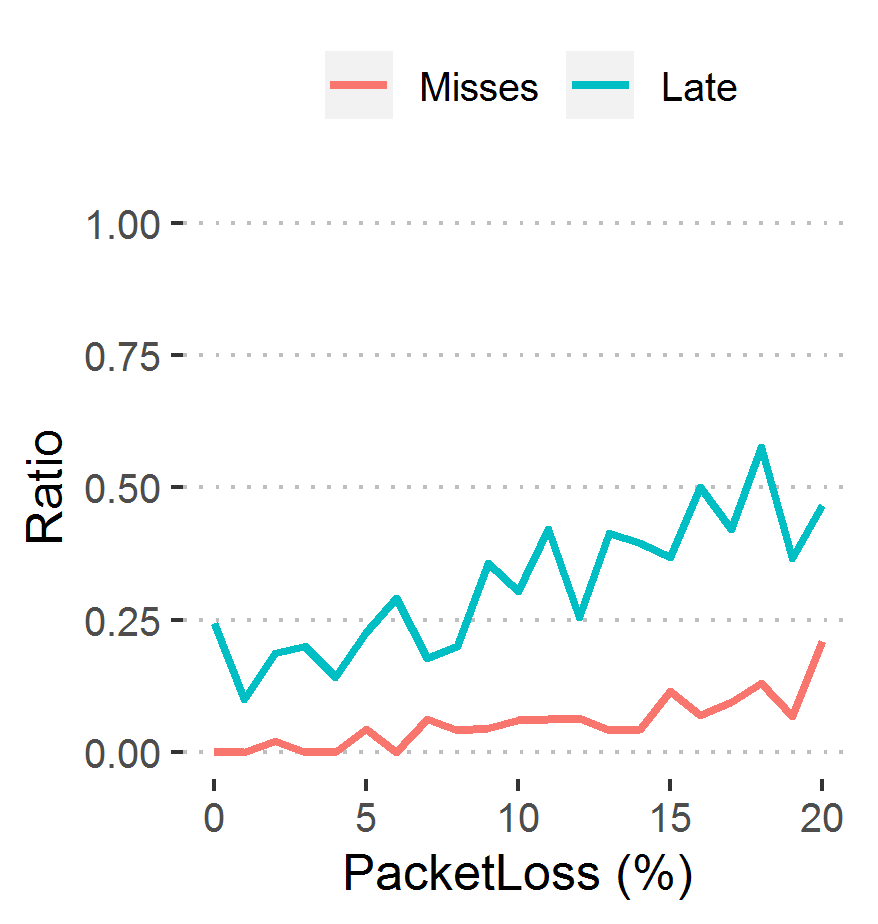
\includegraphics[width=\textwidth]{RatiosVsLoss}
	\caption{The ratios of erroneous collisions to correct collisions and missed collisions to total collisions with varying packet loss.} %As packet-loss increases from $10\%$ to $20\%$ the ratio of erroneous collisions to correct collisions sharply increases as does misses to total collisions. Above $60\%$ packet-loss, all collisions are missed.}
	\label{fig_RatiosVsLoss}
\end{figure}

\begin{figure}
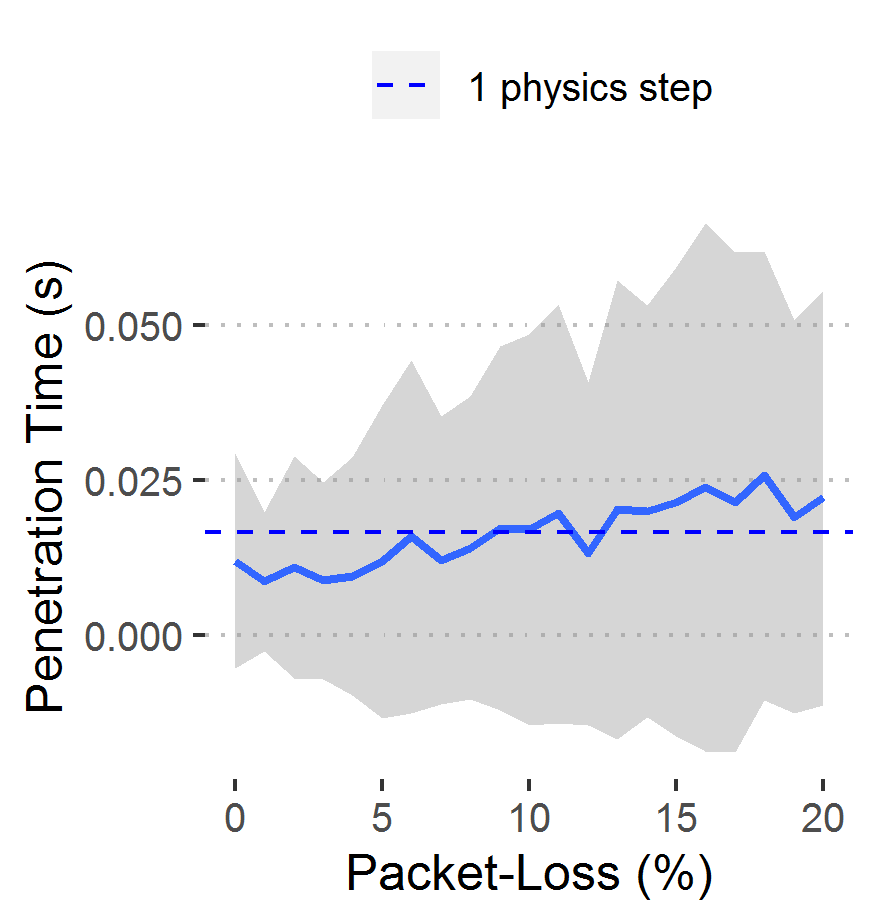
\includegraphics[width=\textwidth]{MeanPenVsLoss}
\caption{Mean penetration time of objects with $+/-2$ standard deviations with varying packet-loss. The maximum expected penetration time of 1 physics steps is marked with a dashed blue line.}
%\caption{Penetration time of objects with varying packet-loss. Each red point represents one or more collisions. The maximum expected penetration time of 1 physics steps is marked with a dashed blue line. The number and magnitude of errors increases as packet-loss increases beyond $10\%$.}
\label{fig_CollisionsPenVsLoss}
\end{figure}

%In addition to varying each aura tolerance factor, an experiment was also carried out to determine the effects of packet-loss on the correctness of collisions between objects. In this experiment the packet-loss was varied from $0\%$ to $80\%$ in increments of $10\%$. Packet-loss is not factored into the aura calculation and therefore has no tolerance. Packet-loss is controlled using the Traffic Control tool; packet-loss is emulated on each server for all communication received from the other server.
%
%RakNet, the library used for network communication in this project, includes a reliability layer. This means if packets are lost and an acknowledgement message is not received, sending will be re-attempted. However, this takes time and therefore causes a delay in messages being received. Delays in messages will lead to erroneous collisions, therefore as packet-loss increases, erroneous collisions should increase in number and magnitude. If messages are delayed enough, the collision will be missed as the two objects pass each other on different servers without ever interacting with each other. 
%
%%TODO: Check if aura updates are ordered, mention that here.
%%RakNet's reliability layer uses best effort, meaning messages are not guaranteed to be received, which means some messages may never be received resulting in 
%
%\begin{figure}
%\centering
%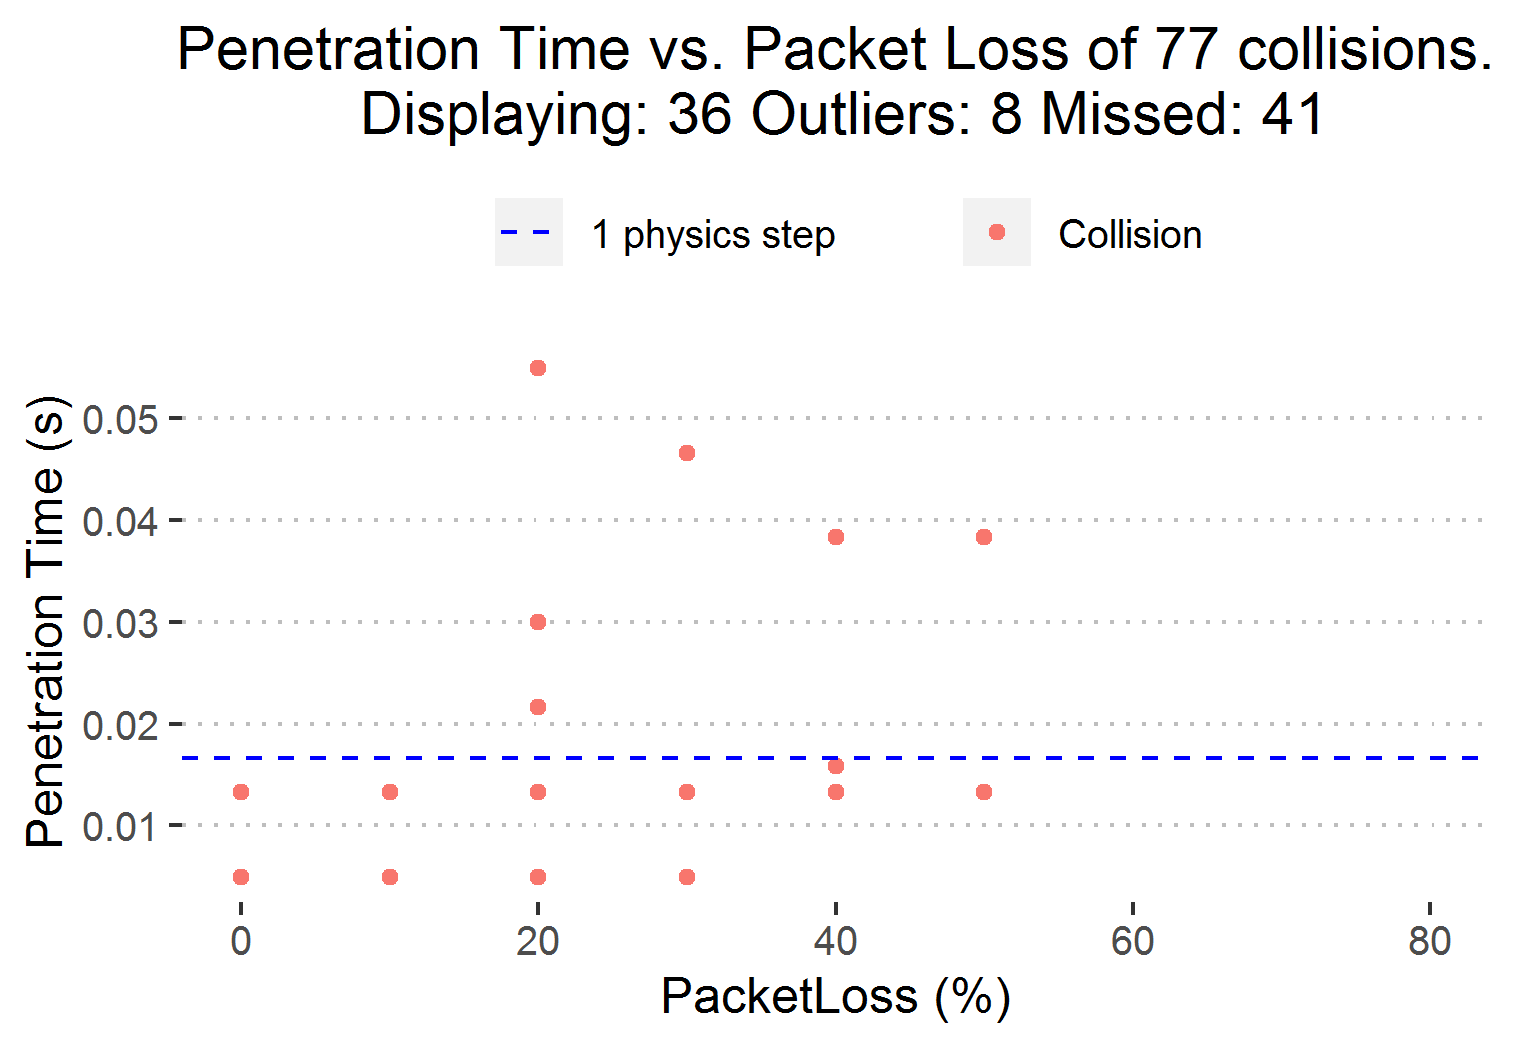
\includegraphics[width=\textwidth]{CollisionsPenVsLoss}
%\caption{Penetration time of objects with varying packet-loss. Each red point represents one or more collisions. The maximum expected penetration time of 1 physics steps is marked with a dashed blue line. The number and magnitude of errors increases as packet-loss increases beyond $10\%$.}
%\label{fig_CollisionsPenVsLoss}
%\end{figure}
%
%\begin{figure}
%\centering
%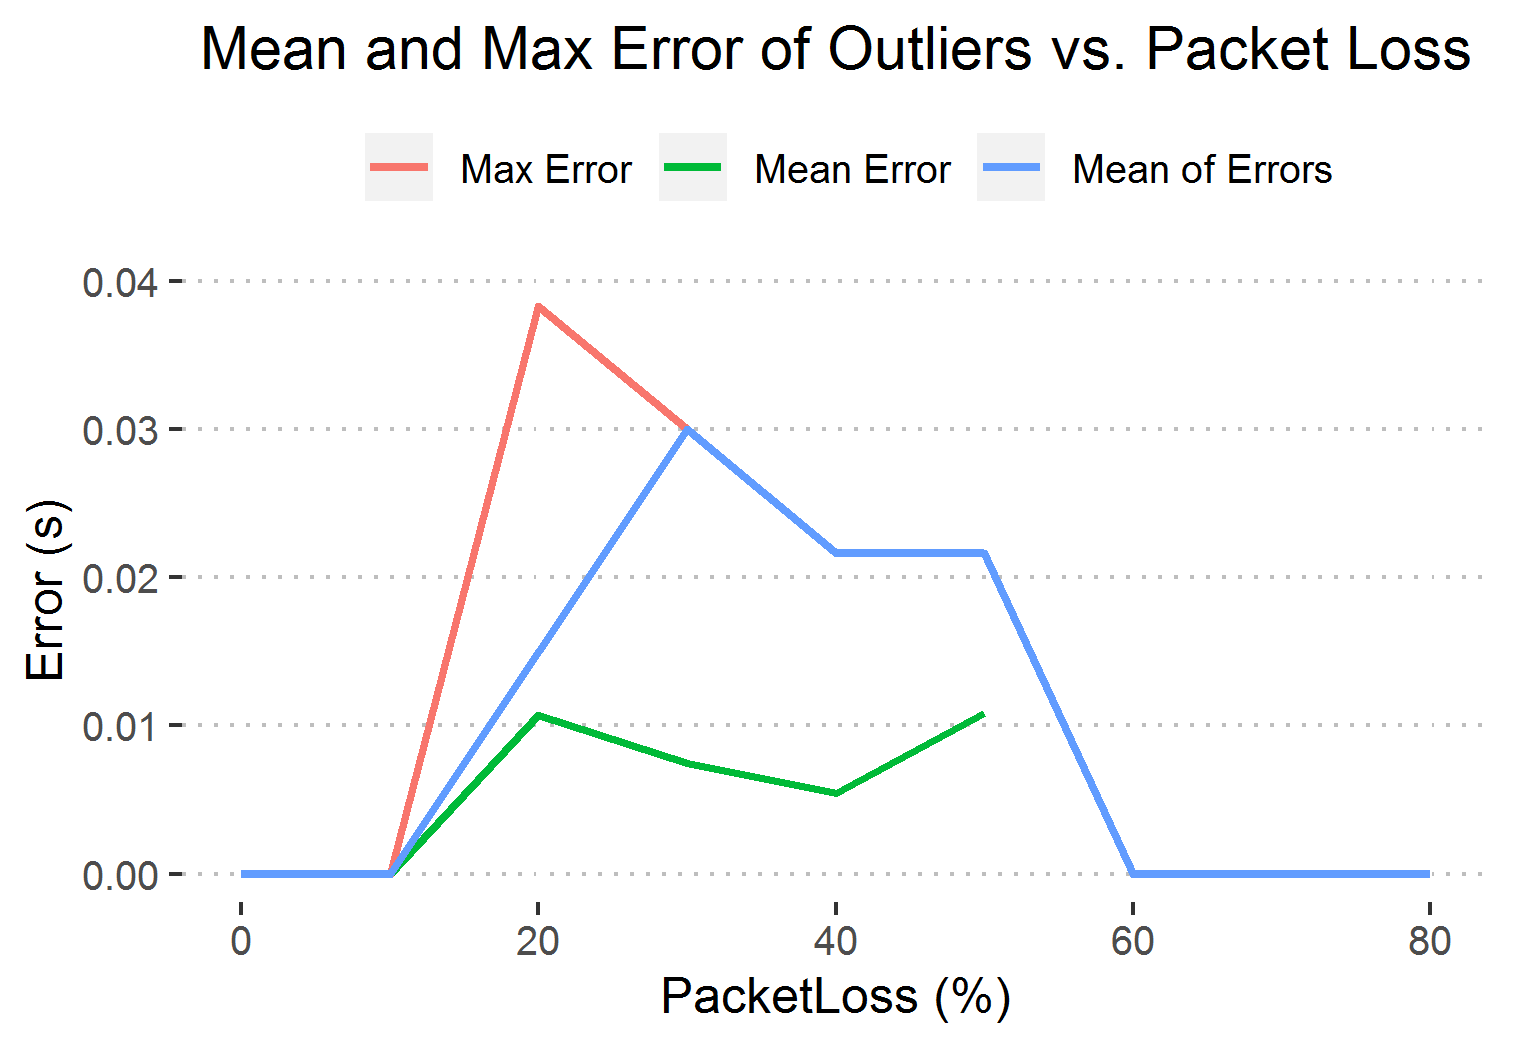
\includegraphics[width=\textwidth]{MeanMaxErrorVsLoss}
%\caption{The mean and max of collision errors with varying packet loss. As packet-loss increases from $10\%$ to $20\%$ the magnitude of errors sharply increases until above $60\%$ where all collisions are missed so there is no error.}
%\label{fig_MeanMaxErrorVsLoss}
%\end{figure}
%
%\begin{figure}
%\centering
%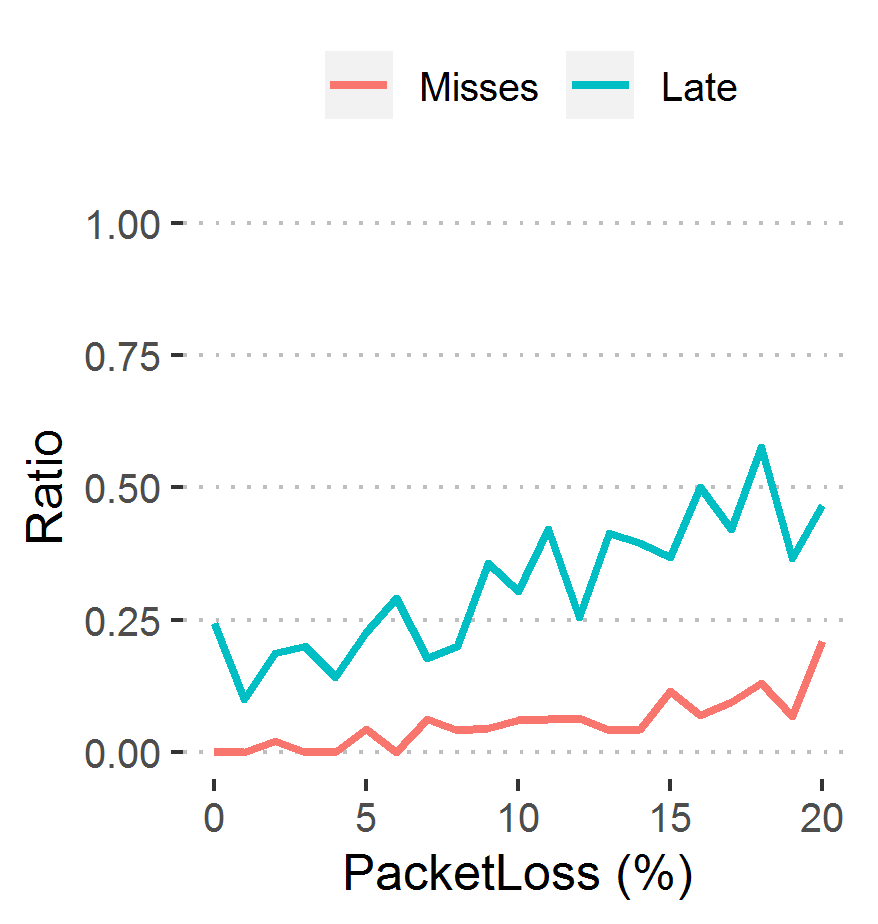
\includegraphics[width=\textwidth]{RatiosVsLoss}
%\caption{The ratios of erroneous collisions to correct collisions and missed collisions to total collisions with varying packet loss. As packet-loss increases from $10\%$ to $20\%$ the ratio of erroneous collisions to correct collisions sharply increases as does misses to total collisions. Above $60\%$ packet-loss, all collisions are missed.}
%\label{fig_RatiosVsLoss}
%\end{figure}

As packet-loss increases, late and erroneous collisions increase and late collisions increase in magnitude. This is due to messages being delayed as packets are lost and need to be re-sent by RakNet's reliability layer. Missed collisions begin to occur as soon as packet-loss exceeds $1\%$, but increase at a lower rate relative to late collisions. (Note, late collisions begin to occur from $0\%$, this is expected as all factors are set to be equal to their tolerances). These results demonstrate that AP is able to prevent $50\%$ of late collisions even in cases of packet-loss as high as (15\%) and prevent all missed collisions with up to $1\%$ packet-loss, which is much greater packet-loss than would be expected in practice (0.01\%) \cite{ThousandEyesCloudPerf2018}.

\chapter{Conclusions and Future Work}
\section{Conclusions}
An approach to networked real-time physics simulations that is scalable and alleviates the processing limitation of a single server has been presented. Only open-source software has been used in our approach and our algorithm has been developed in a way that is agnostic to any specific application technology.

In Chapter \ref{ProbDef} the challenges facing distributed real-time physics were defined, possible solutions were addressed and our chosen solution, AP, was presented and justified. The origination of the aura calculation used for the auras in AP was also presented. The implementation of AP was discussed in Chapter \ref{Implementation}, including potential topologies that could be used by a system using AP and the breakdown of the components of each server. Chapter \ref{Implementation} also gave an overview of the visualiser used by the system, which is responsible for rendering the state of the simulation through the use of replicas. Its features and their implementation details were discussed.

In Chapter \ref{Results}, the design and results of the experiments were presented for addressing the questions set out by this study: "Can scalable real-time physics simulations be achieved?" and "Can real-time physics simulations remain correct when scaled?".

The experiments carried out in this study establish that the approach is scalable, as demonstrated by the addition of servers improving the performance of the system when simulating an increasingly large number of objects. This study has demonstrated that a standard real-time physics engine (in this case, PhysX) may be incorporated into our scalable real-time physics system and achieve performance that is acceptable for real-time distributed simulations such as networked games.

The correctness of collisions in AP have been measured and evaluated. The experiments conducted in this study establish that collisions remain correct in AP, even when objects interact while intersecting the boundary. This has been shown to be true while increasing each of the following factors: speed; latency and frame-time. Collisions remain correct up to the tolerance values for each factor and begin to show errors as soon as the tolerance is exceeded, demonstrating the correctness of the aura calculation used in AP. The holds true if thrashing collisions are excluded from the results. The number of thrashing collisions and amount of times thrashed were both measured, potential solutions to the thrashing problem were proposed in \ref{Thrashing} and we assume that these errors will be fixed in future work.

In addition to the aura factors being tested, the effects of packet loss on the system have also been explored and the limits of AP with increasing packet loss have been shown. This research demonstrates that collisions of rigid-bodies can be handled correctly in a scalable, distributed real-time physics system, even when those collisions take place on or near a server-region boundary.

\section{Future Work}
Work will continue to carry out experiments to determine the effects that changing each of the aura tolerances has on the performance and scalability of AP. Future work will enable each tolerance value to be dynamic and the aura size could adapt with the changing conditions of the system. This would improve performance when factors are low and maintain correctness when factors are high.

Acceleration could also be factored into the aura calculation. The velocity between time steps is often limited and using an acceleration tolerance would allow for smaller auras for slow moving objects. Smaller auras lead to better performance as it leads to fewer aura broadcasts and object migrations. Note that the acceleration tolerance could only apply to the displacement calculation of the local object, as the velocity of a potential remote object is unknown.
%Reference where smaller auras improving performance are explained

An alternative to just aura position and radius being sent over the network would be to send more details of the object projecting the aura. This could include bounding sphere and velocity and would allow the receiving server to determine the size of the aura. Under changing conditions, such as changes in latency the receiving server could dynamically change the size of the auras without the need for the sending server to send the new sizes of the auras.

The implementation of AP could be improved through the separation of the main server update rate and the network tick rate (network update frequency) as discussed in \ref{update-rate-test-values}. These two update rates are often decoupled in video games, as it enables the server to maintain an accurate simulation while allowing for a lower tick rate to reduce the network requirements i.e. bandwidth. A lower frequency tick rate would mean a larger aura is required as there would be a longer delay between aura creation/update/collisions events and messages being sent and a longer delay between a message being received and processed. Larger auras would likely lead to a drop in performance. However, a lower frequency tick rate would mean lower processing overhead for sending, receiving and processing network messages. This trade-off could be investigated to determine how it affects performance of the overall system.

%Future experiments may also involve the decoupling of ``update rate'' from ``tick rate'' as described in Section \ref{update-rate-test-values}. As some video games opt to maintain a high internal tick rate to improve simulation accuracy but use a lower or variable update rate to save bandwidth when communicating with networked peers, it would be of interest to examine how doing so would affect the correctness of aura projection in these configurations.


Scalability could be improved through the use of load-balancing and run-time elastic resources. Server regions could use dynamic boundaries to balance the workload of the simulation between servers. This could make use of existing research into graph-partitioning, where objects are treated as edges and overlapping auras are undirected edges. Boundaries could be moved to reduce the number of boundary-edge intersections. In addition, statistical modelling and analysis could be employed to predict future states of the simulation in order to reduce boundary-edge intersections that will occur. Through the use of elastic resources, it would also be possible to `spin-up' and `wind-down' nodes as required by the simulation. Combined with dynamic boundaries between servers, the simulation workload could be moved to newly created servers, by dividing existing server regions when computational requirements are high. When they are low, the regions from multiple servers could be consolidated into a single server, reducing the number of servers required, resulting in lower financial cost.

%, new regions will need to be created during run-time (either dividing existing regions or expanding the simulation area). New nodes will need to be launched during run-time, using  and a method for re-dividing up the workload between the new and existing nodes will be required. This would require on dem

%Additionally, on-demand dynamic load balancing will be explored to enable improvements in scalability. This will leverage run-time resource (re)allocation in order to maintain efficient distribution of cloud-based processing facilities in response to changes in the simulated environment. Simulations of objects that can freely interact with one another with a high degree of fidelity are never uniform, and therefore on-line statistical modelling and analysis will be fundamental to predicting where additional computational units are required. This will necessitate a transition from fixed world region boundaries to dynamic re-partitioning, which we expect will improve performance by reducing the number of auras being projected and the number of objects being migrated, leading to an overall reduction in bandwidth usage.

The use of containers, such as Docker, for the deployment of AP could also be investigated and compared with the current implementation that uses virtual machine cloud instances. Containers would allow for efficient provisioning and management of compute resources within the system as they enable more precise control over resources allocated. In addition, containers provide faster on-demanding provisioning of resources. Using containers instead of cloud instances may require additional overhead in terms of performance, which could be investigated and the trade-off between cloud instances and the benefits of containers explored.
%The use of modern cloud technologies will also be researched, such as containers and container orchestration in order to facilitate efficient provisioning and management of additional compute resources within a distributed physics simulation. The use of lightweight containers versus virtual machine instances may allow for more precise control of compute resource allocation and faster on-demand provisioning, which would lend itself well to streamed gaming applications.

Future cloud deployment architectures could also be investigated. The use of `overseer' nodes to enable scalability in terms of clients connected could be developed and measured, and their ability to provide a level of fault-tolerance in the event of node failure could be tested. Overseer nodes could also be located at the edge, providing lower latencies for connecting clients, but at the cost of a higher latency between overseer nodes and the cloud-based simulation servers and the other overseer nodes.

%Render nodes
%Edge computing

AP works on the principle that any two bodies that may be interacting are always being simulated on the same server. An alternative technique to this would be Cross-Boundary Interaction, as discussed in \ref{ConsideredSolutions}, allowing for bodies to interact across region boundaries i.e. objects that are being simulated on two different servers interacting over the network. There are likely various advantages and disadvantages of Cross-Boundary Interaction compared to Aura Projection, which could be explored and evaluated. The two solutions may have better performance in different situations (such as a large cluster on either side of a boundary) and a solutions which uses both techniques in different circumstances could be developed.

An important feature of a physics engine is the ability to query the state of the simulation. A typical example of this would be a ray-cast, in which a ray is cast between two points in the simulation space to find intersecting bodies. %Ray-casts are commonly used in first-person shooting games, i.e. a ray is cast from the player's weapon to a given distance, and objects that intersect the ray are returned from the query.
Distributed physics adds an extra level of complexity to this as the query may concern spaces and/or objects being simulated on different servers. In the case of spatially-partitioned solutions, the query could overlap the region boundary and in order for the query to be completed, a round-trip of messages between the two servers would be required. If the query is blocking/synchronous (execution cannot continue until the query is complete), this would introduce a large amount of wait time (at least double the network latency). Another option would be to use asynchronous queries, the results of which get returned using a function callback as soon as the results have been received. However this is more complex than a query on a centralised simulation which can return the results synchronously without any network delay.

Experiments in this study have focused on performance and correctness of AP. Further experiments could be carried out to measure bandwidth requirements of AP in different scenarios as well as the effect of reduced bandwidth on both performance and correctness.

More scenarios could be tested for performance. This study has tested the performance of AP with a $0.5$ ratio of objects near and far from the boundary. Performance is expected to be best when all objects are far from the boundary as almost no message exchange is required between servers, likewise performance is expected to be worst when all objects are near to the boundary and are both `awake' and moving, as this requires the most amount of message exchange and subsequently the highest demand of both network resources and computational overhead from the algorithms used in AP. Investigating different ratios of objects near and far from the boundary, different numbers of moving and `sleeping' objects, or simply an increasing number of objects near the boundary, would determine at what point and under what circumstances AP becomes no longer scalable.

%Constraints
AP is currently limited to the migration of single rigid-bodies between servers. Support for other physical entities such as groups of attached rigid-bodies, soft-bodies and constraints within AP could be added and investigated.



% ********************************** Back Matter *******************************
% Backmatter should be commented out, if you are using appendices after References
%\backmatter

% ********************************** Bibliography ******************************
\begin{spacing}{1.5}

% To use the conventional natbib style referencing
% Bibliography style previews: http://nodonn.tipido.net/bibstyle.php
% Reference styles: http://sites.stat.psu.edu/~surajit/present/bib.htm

\bibliographystyle{apalike}
%\bibliographystyle{unsrt} % Use for unsorted references  
%\bibliographystyle{plainnat} % use this to have URLs listed in References
\cleardoublepage
\bibliography{References/references} % Path to your References.bib file


% If you would like to use BibLaTeX for your references, pass `custombib' as
% an option in the document class. The location of 'reference.bib' should be
% specified in the preamble.tex file in the custombib section.
% Comment out the lines related to natbib above and uncomment the following line.

%\printbibliography[heading=bibintoc, title={References}]


\end{spacing}

% ********************************** Appendices ********************************

\begin{appendices} % Using appendices environment for more functunality

%\include{Appendix1/appendix1}
%\include{Appendix2/appendix2}

\end{appendices}

% *************************************** Index ********************************
\printthesisindex % If index is present

\end{document}
